%=========================================================================
% (c) Radim Loskot, 2014

\chapter{Úvod}
\label{Chapter.Introducion}

Internetové prohlížeče denně umožňují rychle a~pohodlně procházet webový obsah a~tzv. HTML dokumenty. HTML dokumenty nemusí být výhradně umístěny pouze na webu a~na vzdálených úložištích, ale mohou přicházet i v~rámci elektronické pošty nebo být součástí aplikační nápovědy, aj. Pro zobrazování HTML dokumentů používáme HTML zobrazovacích strojů. Jedním takovým strojem je CSSBox.

CSSBox je projekt experimentálního (X)HTML/CSS zobrazovacího stroje napsaného v~čistém jazyce Java. Projekt se snaží vyplnit prostor v~implementacích zobrazovacích strojů v~Javě, jejichž vývoj většinou ustal. Hlavním cílem projektu je poskytnout úplné a~dále zpracovatelné informace o rozložení dokumentu. Vyjma analyzování dokumentu umožnuje již v~samotném základu vizualizovat dokument jako prostý obrázek. V~rámci samostatného podprojektu SwingBox dále díky komponentě \texttt{BrowserPane} přidává pokročilé grafické rozhraní pro zobrazování dokumentu, které dokáže reagovat i na události od uživatele.

V~současné době CSSBox implementuje (X)HTML/CSS 2.1 analyzátor a~výše zmíněné zobrazovací komponenty. Cílem této práce je projekt CSSBox rozšířit o možnost skriptování v~dokumentu a~implementovat vybranou základní množinu skriptovacího jazyka JavaScript. Jakým způsobem bude integrace docíleno, je popsáno v~následující práci.

V~úvodu této práce -- kapitole \ref{Chapter.DependenciesAnalysis.ScriptsInHTML} se pojednává o způsobech, jakými mohou být vloženy do HTML dokumentů skripty, a~je demonstrován referenční přístup pro přidání skriptování do dokumentů podle doporučené specifikace HTML 5. Základní architektura použitých závislostí -- projektu CSSBox a~SwingBox je uvedena v~kapitolách \ref{Chapter.DependenciesAnalysis.CSSBox} a~\ref{Chapter.DependenciesAnalysis.SwingBox}.

Kapitola \ref{Chapter.JavaScriptInJavaAnalysis} je zaměřena na analýzu dostupných skriptovacích strojů v~současnosti a~rozbor jejich API. Kapitola blíže popisuje skriptovací engine Rhino, který byl využit pro implementaci JavaScriptového enginu. V~rámci této kapitoly je představeno i standardní skriptovací Java API, jež lze pro skriptování v~Javě využít.

V~kapitole návrhu -- kapitole \ref{Chapter.Design} je nastíněn základní abstraktní návrh celé integrace nového rozšíření do projektu SwingBox. Postupně jsou ukázány jednotlivé náležitosti, které bude zapotřebí vykonat, aby bylo možné integraci provést. V~závěru \linebreak[4]dokumentu -- kapitole \ref{Chapter.Design.SwingBoxIntegration} je demonstrována „registrace“ samotného rozšíření do projektu SwingBox.

Kapitola implementace -- kapitola \ref{Chapter.Implementation} popisuje již implementované řešení, vytvořené jádro uživatelského agenta a jeho podstatu pro zbylá implementovaná rozhraní (kapitola \ref{Chapter.Implementation.BrowsingCore}). Kapitola též představuje způsob, jakým lze vytvářet konkrétní klientské skriptovací enginy (kapitola \ref{Chapter.Implementation.ScriptingArchitecture}), a zároveň uvádí implementovaný engine JavaScriptu (kapitola \ref{Chapter.Implementation.JavaScriptEngine}). Poslední podkapitola \ref{Chapter.Implementation.DemoApplications} znázorňuje dvě ukázkové aplikace, které sloužily pro předvedení hotové funkčnosti a k otestování implementované podmnožiny JavaScriptu.

Testováním, rozborem a případným rozšířením implementovaného řešení se podrobně zaobírá kapitola XY. V podkapitole XY jsou uvedeny techniky, jakými probíhalo testování a ověření správné funkčnosti. Jelikož bylo žádoucí porovnat implementované řešení s ostatními internetovými prohlížeči, hodnotí kapitola XY implementované řešení z hlediska jeho výkonnosti. Kapitola XY také vytváří souhrn veškeré implementované funkčnosti a klasifikuje kompatibilitu implementovaného řešení. Závěrem jsou v kapitole XY diskutovány některé případné cesty budoucí vývoje.

\chapter{Analýza použitých technik}
\label{Chapter.DependenciesAnalysis}

V~rámci této práce se budeme zabývat integrací podpory skriptování v~JavaScriptu ve stroji CSSBox. Abychom mohli provést návrh knihovny implementující rozšíření stroje CSSBox, je zapotřebí upřesnit, jak jsou skripty v~HTML dokumentech reprezentovány, jak jsou vykonávány a~do jakého rozhraní je budeme integrovat.

Problematikou skriptování v~HTML dokumentech se zabývá kapitola \ref{Chapter.DependenciesAnalysis.ScriptsInHTML}. Na projekt CSSBox, jeho architekturu je zaměřena kapitola \ref{Chapter.DependenciesAnalysis.CSSBox}. Komponenta, která bude použita pro zobrazování HTML dokumentů a~která bude implementovat rozšíření skriptování v~těchto dokumentech, je popsána v~kapitole \ref{Chapter.DependenciesAnalysis.SwingBox}. 

\section{Klientské skripty v~HTML dokumentu}
\label{Chapter.DependenciesAnalysis.ScriptsInHTML}

Klientský skript je program, který může doprovázet HTML dokument nebo být do něj přímo vložen. Skript je vykonáván na straně klienta buď ihned po jeho načtení, po načtení celého dokumentu nebo při výskytu některé události. Skripty mohou:

\begin{itemize}
  \item sloužit k modifikaci obsahu dokumentu;
  \item být spuštěny událostmi ovládacích prvků a~jinými událostmi prohlížeče;
  \item být využity pro validaci a~odesílání obsahu formuláře na server.
\end{itemize}

\noindent Pro vložení nového skriptu do HTML dokumentu a~jeho příp. vykonání máme několik způsobů, např.:

\begin{enumerate}
  \item Uvést skript v~dokumentu ve speciální značce \texttt{<script>};
  \item Vložit skript do atributu určeného pro událostní obslužnou rutinu, který se bude vykonávat vždy po výskytu dané události, např. do atributu \texttt{onclick}.
  \item Vložit skript do dokumentu dynamicky tím, že vložíme do dokumentu pomocí skriptu nový element \texttt{<script>} a~definujeme jeho vykonávací kód.
\end{enumerate}

Skripty ve značkách \texttt{<script>} jsou spouštěny samostatně, vždy pouze jednou a~nikoliv~opakovaně tak jako skripty vytvářené v~atributu pro událostní obslužné rutiny. Během zpracovávání dokumentu jsou jednotlivé skripty v~těch značkách vykonány. Jak a~v~jakém pořadí spouštění skriptů probíhá, popíšeme dále v~této kapitole.

V~rámci samotné značky \texttt{<script>} můžeme podle doporučené specifikace HTML 5 rozlišit celkem 6 atributů. Všechny atributy řídí vykonávání skriptu v~určitém momentu jeho zpracovávání a~jejich dynamická změna nemá žádný efekt na průběh skriptu. Specifikace uvádí následující atributy:

\begin{enumerate}
  \item \textbf{\texttt{src}} -- URL\footnote{URL (Uniform Resource Locator) -- řetězec sloužící k jednoznačné identifikaci zdroje} souboru s externím skriptem;
  \item \textbf{\texttt{type}} -- MIME\footnote{MIME (Multipurpose Internet Mail Extensions) -- internetový standard definující různé typy internetového média} typ skriptu;
  \item \textbf{\texttt{charset}} -- typ kódování souboru s externím skriptem;
  \item \textbf{\texttt{async}} -- udává, zda bude skript spuštěn asynchronně;
  \item \textbf{\texttt{defer}} -- specifikuje odložení spuštění skriptu až do dokončení načtení dokumentu;
  \item \textbf{\texttt{crossorigin}} -- pokud je atribut přítomem, pak bude na server zaslán CORS\footnote{ CORS (Cross-origin resource sharing) -- Mechanismus umožňující stahování zdrojů z více povolených domén než pouze z domény, ze které pochází dotazovaný zdroj.} požadavek. 
\end{enumerate}

Kromě samotných atributů elementu skriptu specifikace HTML 5 doporučuje asociovat s elementem \texttt{<script>} i speciální příznaky. Příznaky jsou nastavovány na základě toho, kde byl element skriptu zpracován a~na základě výše zmíněných atributů. Uvedenými příznaky ve specifikaci jsou:

\begin{enumerate}
  \item \textbf{\texttt{already-started}} -- značí, zda byl skript již vykonán. Při klonování elementu \texttt{<script>} se musí příznak sdílet;
  \item \textbf{\texttt{parser-inserted}} -- příznak je nastaven pro všechny skripty vložené do dokumentu HTML nebo XML parserem, např. při vložení pomocí \texttt{document.write()}. Skripty vložené při vytváření dokumentu nemají tento příznak nastaven;
  \item \textbf{\texttt{force-async}} -- během počátečního zpracování dokumentu je příznak nastaven. Skripty nemají tento příznak nastaven, pokud jsou vytvořeny a~vloženy do dokumentu dodatečně, nebo pokud mají specifikovaný atribut \texttt{async};
  \item \textbf{\texttt{ready-to-be-parser-executed}} -- příznak používaný pouze pro skripty, které byly vloženy dodatečně některým z parserů dokumentu. Příznak je nastaven, pokud dojde k úspěšnému načtení skriptu z externího zdroje;
  \item \textbf{\texttt{script-type a~script-charset}} -- jsou příznaky, které pouze reflektují atributy elementu \texttt{<script>}. Pokud nejsou atributy skriptu nastaveny, nebo jsou nastaveny špatně, pak obsahují tyto příznaky opravené nebo výchozí hodnoty těchto atributů.
\end{enumerate}

Nastavování části výše zmíněných příznaků by měl obsluhovat parser dokumentu během tvorby elementu \texttt{<script>}. Před spuštěním skriptu by se podle specifikace HTML 5 měla provést příprava skriptu. Příprava zahrnuje několik kroků, které nastaví příznaky např. \texttt{script-type} a~\texttt{script-charset}, případně upraví příznaky nastavené parserem. 

Příprava elementu \texttt{<script>} pro jeho budoucí spuštění je provedena, pokud skript nemá nastaven příznak \texttt{parser-inserted} a~pokud nastane:

\begin{enumerate}
  \item vložení elementu požadovaného skriptu do dokumentu,
  \item vložení nového uzlu nebo fragmentu dokumentu do již existujícího skriptu,
  \item nastavení atributu src, který nebyl předtím nastaven.
\end{enumerate}

Prvotní fáze přípravy skriptu, jíž výsledkem je nastavení příznaku \texttt{already-started}, tj., zda je skript spustitelný, je znázorněna v~příloze \ref{Annex.ScriptPreprocessing}. Během přípravy dochází také k~zahájení načítání skriptů z externích zdrojů a~umisťování jejich spuštění do front skriptů ke spuštění, aniž by docházelo k čekání, než jsou skripty kompletně načteny. 

Pokud spouštíme skript existující přímo v~dokumentu, je jeho vykonávání zahájeno ihned a~to i bez ohledu, zda předchozí skripty skončily své provádění. Všechny skripty, které mají uvedený externí zdroj, nejsou \texttt{parser-inserted} a~byly již načteny, jsou spouštěny také okamžitě bez zbytečného čekání. Naopak problematika umísťování blokujících skriptů z důvodu čekání na zpracování stylů nebo \texttt{parser-inserted} skriptů do front skriptů ke spuštění je značně komplikovaná. Více o zpracovávání těchto skriptů si lze dočíst v~samotné specifikaci HTML 5 \cite{Bibliography.HTML5.Scripting}.

\section{Renderovací stroj CSSBox}
\label{Chapter.DependenciesAnalysis.CSSBox}

CSSBox je projekt (X)HTML/CSS renderovacího stroje napsaného v~čistém jazyce Java. Projekt klade velký důraz na poskytnutí informací o zpracovávané stránce.

Renderovací stroj CSSBox očekává na svém vstupu model dokumentu - DOM\footnote{DOM (Data Object Model) -- objektově orientovaná reprezentace XML nebo HTML dokumentu}. Dokument je v~rámci stroje získáván pomocí parseru NekoHTML, ale může být získáván i jiným způsobem. Rozhraním pro všechny zdroje dokumentu je abstraktní třída \texttt{DOMSource}. Pro zpracování stylů dokumentu slouží třída \texttt{DOMAnalyzer}, která převede aktuální dokument na rozložení stránky. Výsledný model rozložení stránky se využívá pro zobrazení stránky, v~knihovně je pro tento účel implementována komponenta \texttt{BrowserCanvas}.

\begin{figure}[H]
  \begin{center}
    \scalebox{0.65}{
      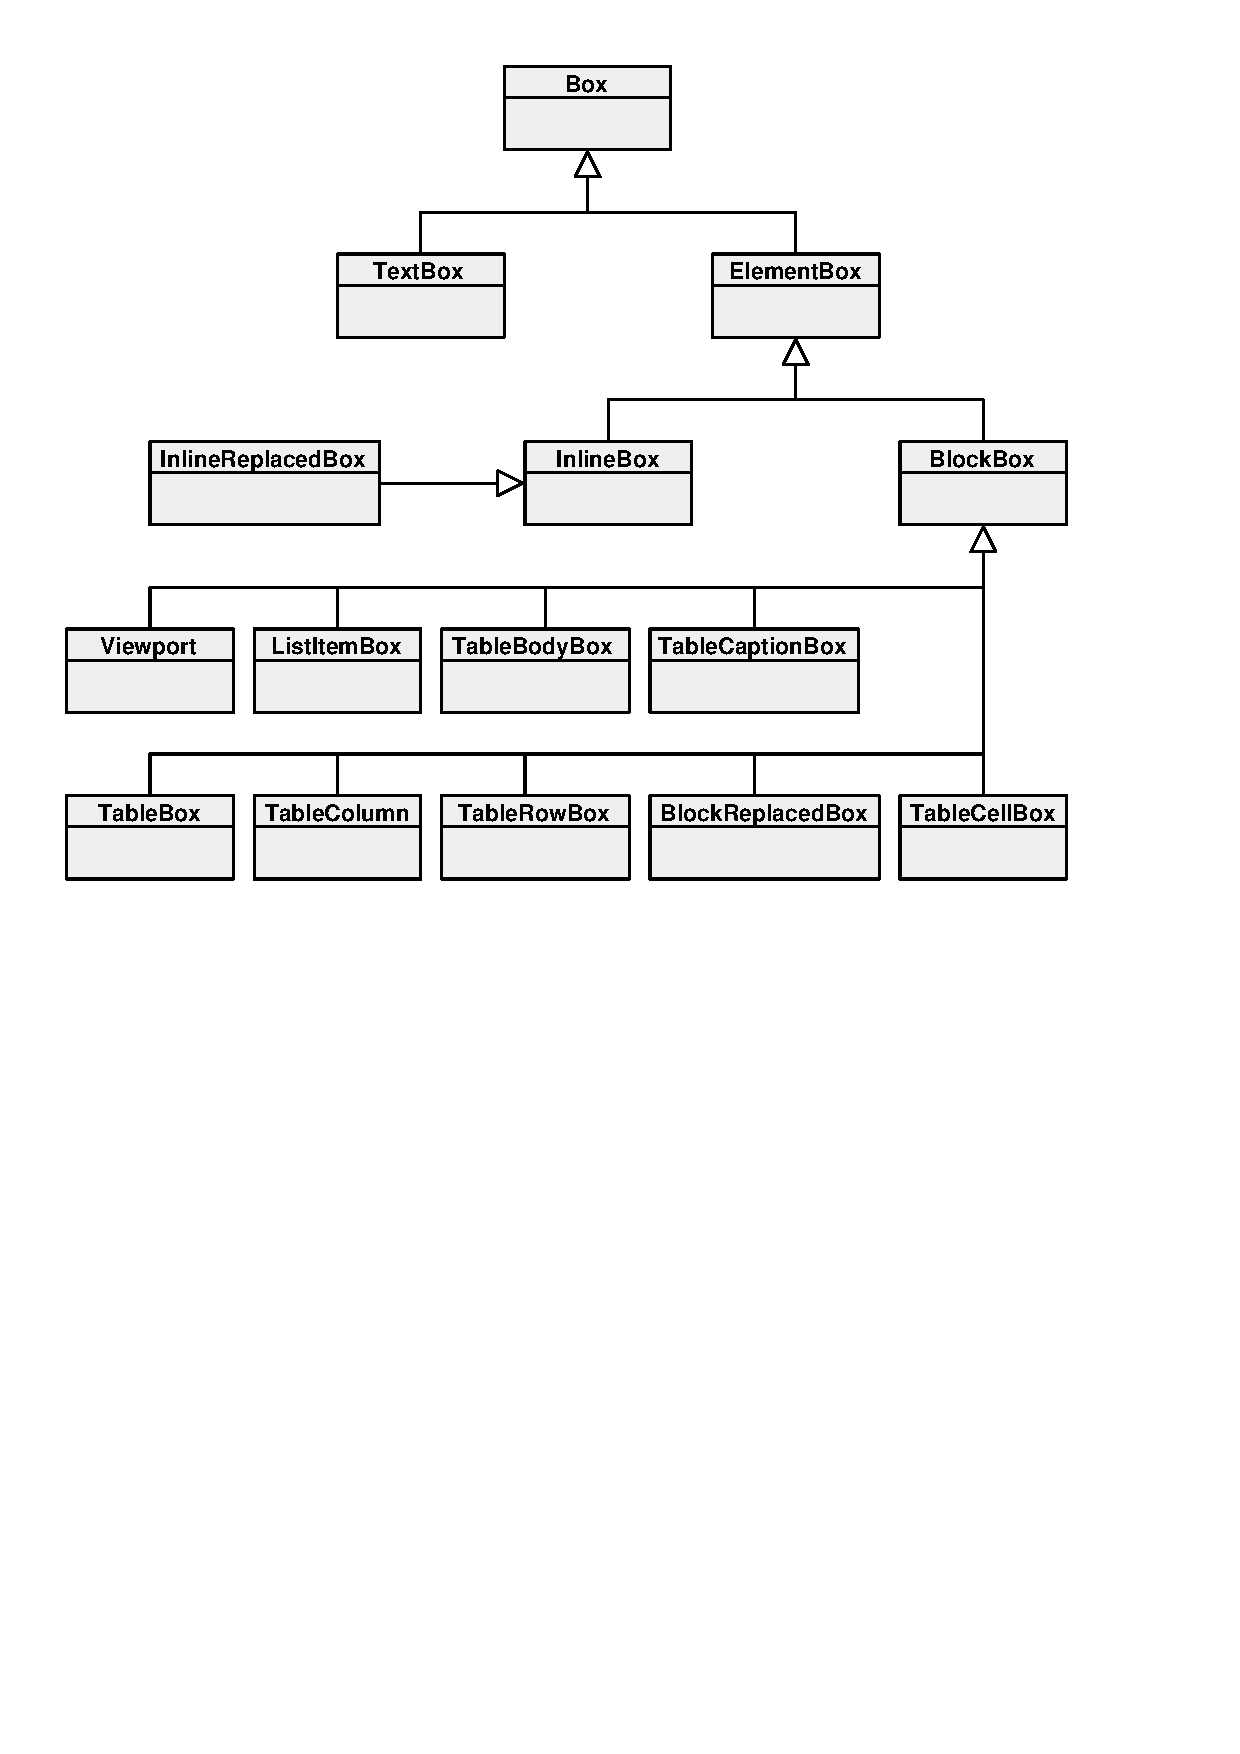
\includegraphics{fig/cssbox.pdf}
    }
    \caption{Hierarchie zobrazovacích komponent třídy \texttt{Box}}
    \label{Figure.BoxHierarchy}
  \end{center}
\end{figure}

Komponenta \texttt{BrowserCanvas} vytváří strom vykreslených objektů třídy Box. Strom je vytvářen ze vstupního dokumentu a~výstupu analyzátoru stylů. Ke každému vykreslovanému elementu dokumentu, je vytvořen třídou \texttt{BrowserCanvas} jeho odpovídající \texttt{Box}. Každý prvek HTML stránky se pojí se specializovanou třídou \texttt{Box}, jak je znázorněno na obrázku \ref{Figure.BoxHierarchy}. Typ boxu nemusí být určen pouze typem elementu dokumentu, ale i jeho styly. Pokud blokový prvek má nastaveno zobrazení na řádku, tak bude ve stromu reprezentován třídou \texttt{InlineBox} a~nikoliv~třídou \texttt{BlockBox}. 

\clearpage

\section{Projekt SwingBox}
\label{Chapter.DependenciesAnalysis.SwingBox}

V~rámci podprojektu SwingBox, který je součástí projektu CSSBox, byla vyvinuta komponenta \texttt{BrowserPane} \cite{Bibliography.SwingBox.Thesis}, která rozšiřuje funkčnost základního zobrazování dokumentu komponentou \texttt{BrowserCanvas}. Komponenta \texttt{BrowserPane} vychází ze třídy \texttt{JEditorPane}, ve které předefinovává výchozí zobrazování (X)HTML dokumentů. Pro zobrazování těchto dokumentů využívá třídu \texttt{SwingBoxEditorKit}, která zařizuje veškerou logiku zobrazování.

Komponenta \texttt{BrowserPane} umožňuje načítat dokumenty předáním jejich URL adresy, předáním dokumentu jako textový řetězec, nebo předání vstupního streamu s dokumentem. Na základě typu dokumentu, který má být zobrazen, komponenta dále volá pro čtení dokumentu odpovídající kit -- v~našem případě \texttt{SwingBoxEditorKit}. Kit zařizuje s použitím třídy \texttt{ContentReader} načtení rozvržení stránky (viz kapitola \ref{Chapter.DependenciesAnalysis.CSSBox}) a~jeho převod na reprezentaci dokumentu \texttt{SwingBoxDocument}, tak jak ho přijímá rozhraní komponenty \texttt{JEditorPane}. Třída \texttt{ContentReader} provádí převod rozvržení stránky na prvky dokumentu, tzn., převádí objekty třídy \texttt{Box} na objekty třídy \texttt{ElementSpec}. Veškeré načítání dokumentu ve formě DOM a~jeho rozvržení třídou \texttt{DOMAnalyzer}, je prováděno ve třídě \texttt{CSSBoxAnalyzer}, na kterou je reference uvnitř třídy \texttt{ContentReader}.

\begin{figure}[H]
  \begin{center}
    \scalebox{0.70}{
      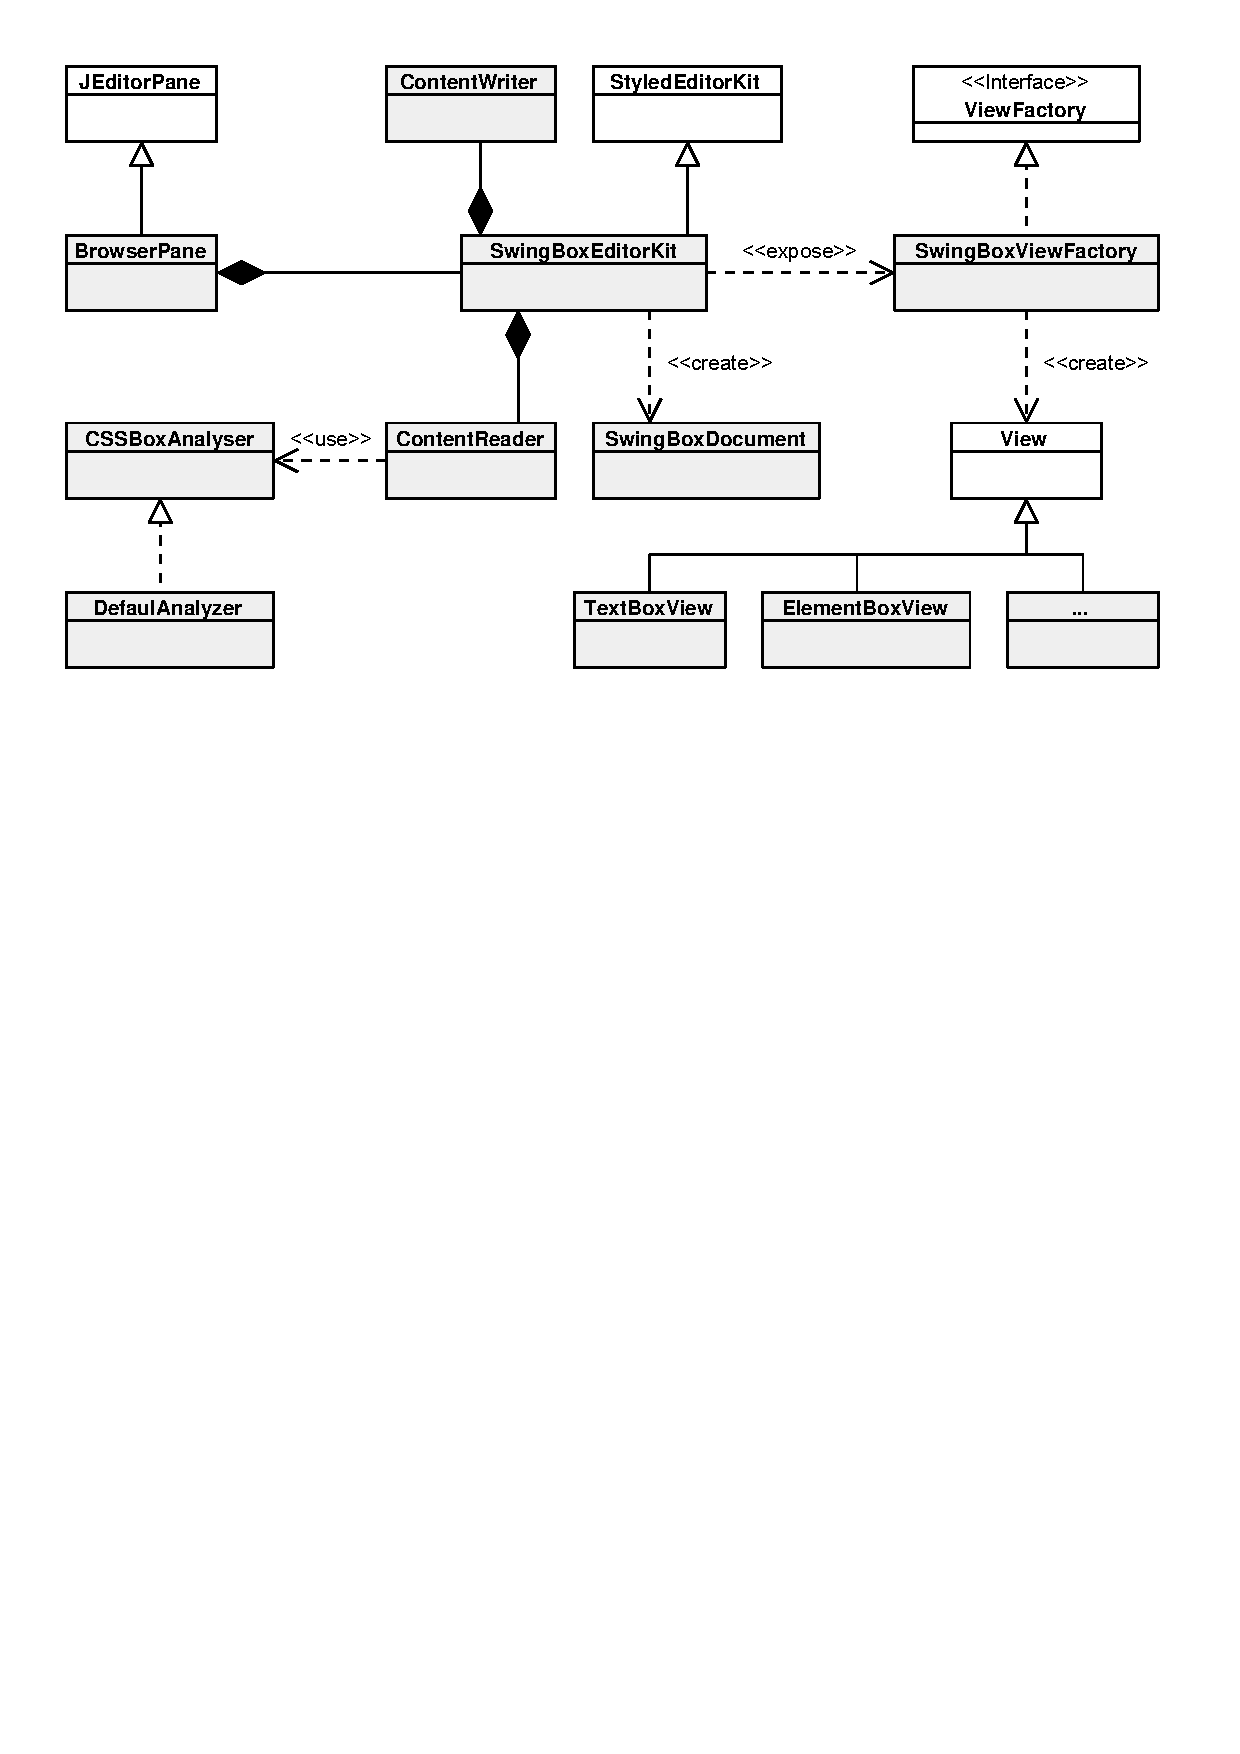
\includegraphics{fig/swingbox.pdf}
    }
    \caption{Diagram tříd komponenty \texttt{BrowserPane}}
    \label{Figure.SwingBoxDesign}
  \end{center}
\end{figure}

Prvky dokumentu \texttt{SwingBoxDocument}, které vytváří třída \texttt{ContentReader}, jsou vykreslovány na zobrazovací plochu \texttt{BrowserPane} ve formě pohledů \texttt{View}. Vykreslování řídí automaticky komponenta \texttt{JEditorPane}, která zná referenci na továrnu pohledů \linebreak\texttt{SwingBoxViewFactory}. Továrna pohledů je používaná komponentou \texttt{JEditorPane} vždy při potřebě vykreslit požadovaný dokument. Továrna se využívá pro vytváření pohledů pro každý prvek dokumentu \texttt{SwingBoxDocument}. Jelikož prvky dokumentu \texttt{ElementSpec} v~sobě zapouzdřují informaci o tom, jaký box obalují, je možno vytvořit pohledy, které přesně korespondují s množinou boxů uvedených v~kapitole \ref{Chapter.DependenciesAnalysis.CSSBox}.

\chapter{Analýza podpory skriptování v~jazyce JavaScript v~Javě}
\label{Chapter.JavaScriptInJavaAnalysis}

Tato kapitola se zabývá analýzou skriptování a~nástrojů, které lze využít pro tvorbu skriptů. Zaměřuje se na skriptovací jazyk JavaScript a~jeho použití v~Java aplikacích. Kapitola záměrně popisuje zejména skriptovací stroj Rhino a~standardní skriptovací Java API, jež lze pro skriptování použít.

Skriptovací jazyky jsou programovací jazyky, které nám umožňují psát tzv. skripty. Na rozdíl od kompilovatelných zdrojových kódů, je kód skriptu vyhodnocován a~interpretován tzv. virtuálním strojem -- za běhu skriptu. Většina skriptovacích jazyků je typována dynamicky za běhu skriptu, což nám umožnuje vytvářet proměnné bez specifikace typu, neboť typová konverze je prováděna automaticky. V~dynamických jazycích můžeme použít jednu proměnnou pro uložení více typů. Skriptovací jazyky mají jednoduchou syntaxi, což umožňuje v~určitých případech vyřešit poměrně složité problémy pomocí relativně krátkého kódu, efektivně a~poměrně v~krátkém čase.

Ačkoliv~jsou skripty obvykle kompilovány za běhu skriptu, lze je zkompilovat do mezikódu Javy a~nechat je vykonat JVM\footnote{JVM  (Java Virtual Machine) -- virtuální stroj Javy zpracovávající mezikód jazyka Java (Java bytecode)}. V~Javě bylo implementováno mnoho skriptovacích Jazyků, využívajících různá rozhraní pro skriptování, což bylo mj. i důvodem pro vznik obecného skriptovacího Java API (viz kapitola \ref{Chapter.JavaScriptInJavaAnalysis.ScriptingJavaAPI}). Mezi nejrozšířenější skriptovací jazyky pro Javu můžeme zařadit BeanShell, s velmi podobnou syntaxí jakou disponuje Java, a~další implementace již existujících jazyků v~Javě jako je např. Jython -- implementace Pythonu,  JRuby -- implementace Ruby, Groovy aj.

Interpretů JavaScriptu implementovaných v~Javě běžících na JVM není mnoho. Z důvodu výkonnosti je většina interpretů JavaScriptu pro webové prohlížeče napsána nativně v~C nebo C++ a~využívá JIT\footnote{JIT (Just in Time) -- metoda překladu urychlující běh skriptu překladem kódu do strojového jazyka} techniky. Jmenovitě nejznámější nativní javasriptová jádra jsou z rodiny „Monkey“, kterou spravuje společnost Mozilla, a~která jsou postupně využívána ve webovém prohlížeči Firefox. Dalšími jádry ostatních webových prohlížečů je V8 použité v~Google Chrome, Carakan v~Opeře, Chakra v~Iternet Exploreru nebo JavaScriptCore v~prohlížeči Safari.

Nejvíce používané interprety cílené pro Java aplikace máme v~současnosti pouze tři. Nejznámějším interpretem je již zmíněné Rhino (kapitola \ref{Chapter.JavaScriptInJavaAnalysis.Rhino}) \cite{Bibliography.Rhino.Docs}, které je i dodáváno v~Oracle implementaci JDK\footnote{JDK (Java Development Kit) -- balík základních nástrojů potřebných pro vývoj aplikací pro platformu Java} 6 a~7, kde realizuje výchozí skriptovací stroj pro Javu. Dalším interpretem s velkým budoucím potenciálem, který bude součásti Oracle implementace JDK 8 a~který je stále ve vývoji, je interpret Nashorn \cite{Bibliography.Nashorn.Project} (kapitola \ref{Chapter.JavaScriptInJavaAnalysis.Nashorn}). Oba zmíněné skriptovací jazyky implementují standardní skriptovací Java API. Rhino bylo o skriptovací API rozšířeno firmou Sun, kdežto Nashorn je vyvíjen s tímto API zprvu počátku. Posledním a~nepříliš používaným interpretem je YAJI \cite{Bibliography.YAJI.Project}, který se snaží oživit starý interpret FESI \cite{Bibliography.FESI.Project} tím, že do něho přidává většinu vlastností z nejnovější specifikace ECMAScriptu.

\section{Rhino}
\label{Chapter.JavaScriptInJavaAnalysis.Rhino}

Rhino je implementace javasriptového jádra napsaná v~programovacím jazyce Java. Projekt Rhina byl zahájen v~roce 1997 firmou Netscape, kdy firma potřebovala integrovat podporu JavaScriptu do budoucího prohlížeče založeném na platformě Java \cite{Bibliography.Rhino.History}. Rhino vzniklo portem nativní knihovny SpiderMonkey, takže i nyní si lze v~kódu nevšimnout Java ekvivalentů nepodmíněných skoků \cite{Bibliography.Rhino.History}.

Projekt prohlížeče, tzv. Javagatoru, byl ovšem brzy pozastaven a~Rhino zůstalo dále jen velmi pozvolna vyvíjené několika vlastníky, včetně společnosti Sun \cite{Bibliography.Rhino.History}. V~roce 1998 bylo Rhino uvolněno společnosti Mozilla a~držitelé licencí se dohodli, že vydají Rhino jako svobodný software \cite{Bibliography.Rhino.History}. Nyní je Rhino spravováno společností Mozilla.

\subsection{Vlastnosti Rhina}
\label{Chapter.JavaScriptInJavaAnalysis.Rhino.RhinoFeatures}

V~současnosti je vydáno Rhino s označením 1.7R4 \cite{Bibliography.Rhino.v17R3,Bibliography.Rhino.v17R4}. Nejnovější verze implementuje všechny vlastnosti Javasriptu 1.7, tzn. je plně ekvivalentní s 3. vydáním standardu \linebreak ECMA-262 ECMAScript a~přidává některé nové vlastnosti, jako jsou doplňky pro práci s poli a~podpora E4X\footnote{Rozšíření programovacího jazyka ECMAScript, které přidává podporu nativního XML a~vychází z normy ECMA-357 ECMAScript pro XML.}. Od verze 1.7R3 Rhino přidává i částečnou podporu Javasriptu 1.8 a~5. vydání ECMAScriptu, která byla nejnovější verzí 1.7R4 zejména optimalizována a~jen mírně rozšířena.

Významnou předností Rhina je jeho dobrá provázanost s Javou. Napojení na jazyk Java a~umožnění hostování objektů Javy nám zpřístupňuje z kódu JavaScriptu používat téměř libovolný balíček a~třídu z Javy. Výjimky pro třídy, které by neměly být zpřístupňěny jsou definované bezpečnostními politikami ve třídě \texttt{SecurityManager} (Java API) a~dodatečně třídou \texttt{ClassShutter} (knihovna Rhino). Jamile je přístup do třídy povolen, lze z kódu JavaScriptu tuto třídu konstruovat, volat její libovolnou metodu či přistupovat k~atributům třídy. Aby bylo možné objekt Javy v~JavaScriptu používat, musí vždy implementovat rozhraní \texttt{Scriptable} (viz kapitola \ref{Chapter.JavaScriptInJavaAnalysis.Rhino.ScriptingWithRhino}).V~případě hostování jazyka Javy, je rozhraní \texttt{Scriptable} implementováno automaticky pomocí třídy \texttt{WrapFactory}. 

Mezi další přednosti Rhina patří možnost rozdělení skriptů do modulů, tak jak bylo specifikováno skupinou CommonJS\footnote{CommonJS -- Skupina lidí snažící se vytvořit jednotné JavaScriptového prostředí pro servery, desktopy a~prohlížeče.} a~možnost vysledovat zdroj odkud skript pochází a~zpracovávat skript podle odpovídající bezpečnostní politiky. Bezpečnostní politiky v~Rhinu vycházejí z Netscape Navigatoru a~jejich aplikace je založená na kontrole URL zdroje \cite{Bibliography.Rhino.Overview}.

Rhino umožňuje dva režimy -- interaktivní a~kompilovaný. V~kompilovaném módu je kód přeložen do mezikódu Javy a~interpretován dále v~JVM. V~interaktivním módu je skript spouštěn jednoduchým interpretem, aniž by docházelo ke generování mezikódu Javy.

Poslední zajimavou vlastností knihovny Rhino je poskytování z kódu JavaScriptu podpory pro implementaci rozhraní a~abstraktních tříd Javy. Implementaci nedefinovaných metod z JavaScriptu zajišťuje třída objektového adaptéru \texttt{JavaAdapter}. Adaptér vytváří pomocí reflexe objekty Javy a~implementuje do objektů navíc metody rozhraní \texttt{Scriptable}, čímž zpřístupňuje tyto objekty pro přímé použití ve skriptech JavaScriptu. Adaptér můžeme buď přímo zavolat nebo ho nechat Rhino automaticky odvodit. 

%\begin{table}[ht] 
%    \texttt{\begin{tabbing}
%      	{ }{ }{ }{ }{ }\={ }{ }\=\+\kill
%      	// přímé zavolání adaptéru \\
%      	\textbf{var} arr1 = \textbf{new} JavaAdapter(java.util.ArrayList, {}); \\
%		// automatické odvození -- Rhino zavolá adaptér automaticky \\
%		\textbf{var} arr2 = \textbf{new} java.util.ArrayList();
%    \end{tabbing}}
%\end{table}
%\vspace{-12mm}
%\begin{algoritmus}
%	\caption{Demonstrace explicitního a~implicitního volání adaptéru Javy}
%	\label{Algorithm.JavaAdapterInRhino}
%\end{algoritmus}

\subsection{Skriptování s Rhinem}
\label{Chapter.JavaScriptInJavaAnalysis.Rhino.ScriptingWithRhino}

Zdrojové kódy Rhina jsou strukturovány do několika hlavních balíků. Pro konstrukci skriptů v~Javě využijeme hlavně veřejné API z balíku \texttt{org.mozilla.JavaScript}.

Základním prvkem pro spuštění jakéhokoliv~skriptu je objekt třídy Context, jenž nese vláknově specifické informace o prostředí pro běh skriptů. Každé programové vlákno, které vyžaduje spuštění skriptu, by si mělo asociovat vlastní kontext zavoláním \texttt{Context.enter()} a~uvolnit zavoláním \texttt{Context.exit()} \cite{Bibliography.Rhino.ScopesAndContexts}.

Úložiště pro objekty nejvyšší úrovně nazýváme v~JavaScriptu jako tzv. scope. Do scopu vkládáme všechny vlastní objekty. Scope představuje jakousi množinu objektů. Objekt scopu je v~Rhinu klasický JavaScriptový objekt, který implementuje třídu \texttt{Scriptable} a~jenž by měl obsahovat základní stadardní objekty \texttt{Object} a~\texttt{Function}. Inicializovaný scope můžeme získat zavoláním metody \texttt{initStandardObjects()} objektu kontextu. Důležitou vlastností scopu je, že je kontextově nezávislý, i přestože scope může být vytvořen z kontextu \cite{Bibliography.Rhino.ScopesAndContexts}. Scope vytvořený jedním kontextem můžeme vyhodnotit s využitím jiného kontextu. Ve vícevláknových aplikacích lze nechat jeden scope vyhodnotit více odlišnými kontexty zároveň. Rhino zajištuje, že přístup k vlastnostem objektu je atomický.

Objekty Javy, které chceme zpřístupnit do kódu skriptu, by měly implementovat rozhraní \texttt{Scriptable} a~poskytnout metody pro práci s vlastnostmi objektu: \texttt{get()}, \texttt{put()}, \texttt{has()} a~\texttt{delete()}. Základní implementaci rozhraní \texttt{Scriptable} a~přístup k atributům objektu pomocí hashovací tabulky poskytuje v~Rhinu třída \texttt{ScriptableObject}. Kromě toho třída \texttt{ScriptableObject} implementuje některé důležité metody pro definování hostovaných objektů z balíků Javy, jako je např. statická metoda \texttt{defineClass()}.

Posledním důležitým rozhraní je rozhraním \texttt{Function}. které je implementováno všemi funkčními objekty Javasriptu. Pokud chceme funkci zavolat, můžeme k tomu použít metody \texttt{call()} nebo \texttt{construct()} v~závislosti na tom, jestli funkce má být volání s klíčovým slovem \texttt{new}.

JavaScript kromě základního objektu Object, který musí v~Javě implementovat již zmíněné rozhraní \texttt{Scriptable}, obsahuje i 5 primitivních datových typů. Tyto datové typy musí být mapovány do Javy na odpovídající třídy. Jakým způsobem je mapování docíleno, je znázorněné v~tabulce \ref{Table.JavaScriptToJavaMapping}. 

\begin{table}[H]
  \begin{center} 
    \begin{tabular}{| c | l |} \hline
    \textbf{Typ v~JavaScriptu} & \textbf{Reprezentace v~Javě} \\ \hline
    \texttt{Undefined} & \texttt{org.mozilla.JavaScript.Undefined} \\ \hline
    \texttt{Null} & \texttt{null} \\ \hline
    \texttt{Boolean} & \texttt{java.lang.Boolean}  \\ \hline
    \texttt{Number} & \texttt{java.lang.Number} \\ \hline
    \texttt{String} & \texttt{java.lang.String} \\ \hline
    \end{tabular}
    \caption{Mapování primitivních typů JavaScriptu do Javy (XXXXXXXXXXXXXXXXXXXXXXXXXXXXXXXXXXXXXXXXXXXXXXXXXXXXXXXXXXXXXXXXXXXXXXXXXXXXXXXX)}
    \label{Table.JavaScriptToJavaMapping}
  \end{center}
\end{table}

\subsection{Princip kompilátoru a~interpretu}
\label{Chapter.JavaScriptInJavaAnalysis.Rhino.CompilerTechniques}

V~předchozí kapitole jsme zmínili sadu nejdůležitějších tříd a~rozhraní z veřejného API Rhina. V~balíku \texttt{org.mozilla.JavaScript} se ovšem nachází i jednotlivé části zajišťující samotnou funkci překladače a~interpretu JavaScriptu.

Mezi nejpodstatnější neveřejné třídy v~balíku patří např. třída \texttt{ScriptRuntime} obsahující metody využívané interpretem a~optimalizátorem jazyka pro generování mezikódu Javy. Formát mezikódu lze konkrétně nalézt v~balíku \texttt{src.org.mozilla.classfile}. Překlad JavaScriptu do bajkódu probíhá běžně za běhu programu. Explicitní překlad skriptu a~vytvoření .class souboru lze vynutit zavoláním překladače JavaScriptu, příkazem:

\medskip
\centerline{\texttt{java org.mozilla.JavaScript.tools.jsc.Main script.js}}
\medskip

Vlastní překladač do bajkódu Javy je velkým specifikem Rhina. Pro každý zkompilovaný skript je vygenerována přesně jedna odpovídající třída v~Javě, která implementuje rozhraní Script. Skript lze potom vykonat zavoláním metody \texttt{exec()} rozhraní Script.

Interaktivní (nekompilovaný) režim interpretu JavaScriptu zajišťuje třída \texttt{Interpret}, která je umístěná také v~hlavním balíku. Interpret JavaScriptu v~Rhinu je klasický zásobníkový automat. Pro reprezentaci mezikódu se používá instrukce s proměnlivou délkou. Instrukce se skládá z operačního kódu a~případných operandů. Prováděcí smyčku interpretu implementuje metoda \texttt{interpretLoop()}, která přijímá aktuální rámec volání a~kontext, ve kterém interpretování probíhá. Rámec volání obsahuje typické položky jako zásobník hodnot, pole symbolů a~aktuální scope objekt.

Zajímavostí interpretu je zavedení dvou druhů zásobníků -- hlavního a~číselného. Hlavní zásobník je určen pro obecné hodnoty, tzn. pro hodnoty všech typů JavaScriptu. Číselný zásobník slouží pro uložení hodnot JavaScriptového primitivního typu \texttt{Number}. Hlavní zásobník je implementován v~Javě jako pole objektů \texttt{Object} a~číselný jako pole primitivního typu \texttt{double}. Mezi hlavním a~číselným zásobníkem probíhá mapování. Pokud je v~hlavním zásobníku uložená unikátní hodnota \texttt{DBL\_MRK}, tak bude čtení odpovídajících hodnot pokračovat ve druhém zásobníku (viz obrázek \ref{Figure.RhinoStack}). Tato technika byla zavedena čistě z důvodu optimalizace, aby nedocházelo ke zbytečnému \csuv{zabalení} primitivního typu do objektu a~aby se šetřila alokace paměti pro objekt a~příp. dereference ukazatelů.

\begin{figure}[H]
  \begin{center}
    \scalebox{0.40}{
      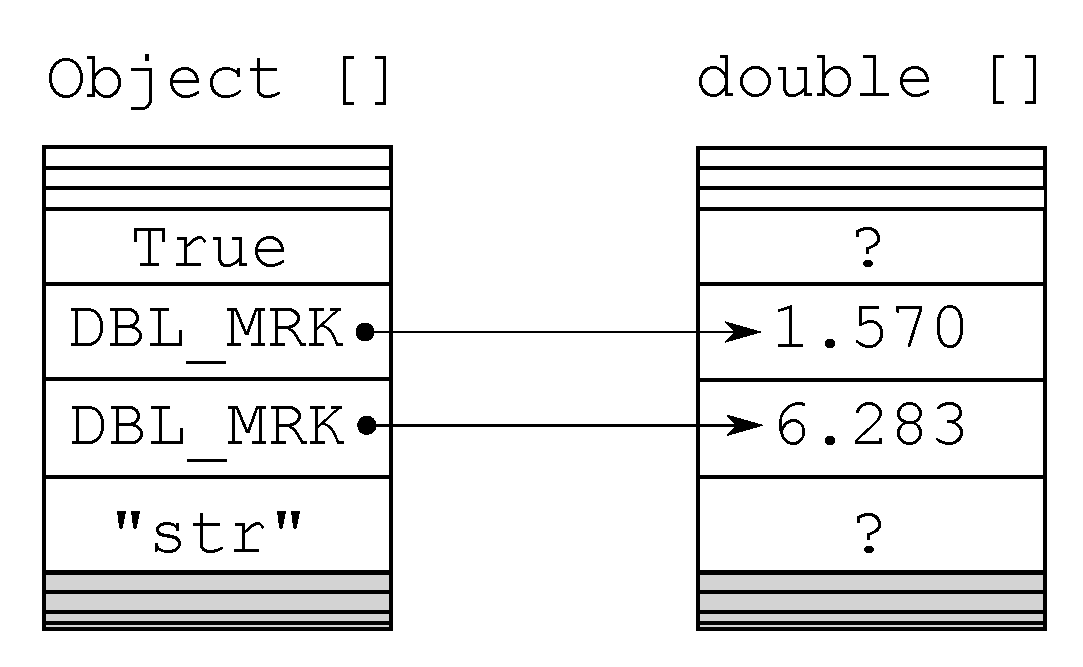
\includegraphics{fig/rhino_stack.pdf}
    }
    \caption{Znázornění koexistence hlavního a~číselného zásobníku}
    \label{Figure.RhinoStack}
  \end{center}
\end{figure}

Interpret JavaScriptu přijímá mezikód jazyka, který je generován metodou compile třídy \texttt{CodeGenerator}. Generátor mezikódu pracuje s abstraktním syntaktickým stromem tvořeným z prvků definovaných v~balíku \texttt{org.mozilla.JavaScript.ast} a~generovaným třídou \texttt{Parser}.

\section{Nashorn}
\label{Chapter.JavaScriptInJavaAnalysis.Nashorn}

Nashorn je projekt, který si klade za cíl vyvinout zcela nový, odlehčený a~výkonný JavaScriptový runtime pro nativní JVM \cite{Bibliography.Nashorn.Project}. Výstupem projektu by měla být schopnost spouštět JavaScriptový kód příkazem jrunscript, která podléhá specifikaci JSR 223\footnote{JSR 223 -- specifikace definující framework pro vkládání skriptů do zdrojového kódu Javy}. Oproti poměrně letitému JavaScriptovému interpretu Rhina vyvinutému pro tehdejší JVM, se Nashorn zaměřuje na nové techniky používání dynamických jazyků v~Javě a~vychází ze specifikace \linebreak tzv. Da Vinci stroje (JSR 292\footnote{JSR 292 -- specifikace pro rozšíření JVM o nativní podporu dynamických jazyků}) \cite{Bibliography.Nashorn.Project}.

Jádro interpretu Nashorn vychází z ECMAScriptu verze 5.1. Skripty jazyka JavaScript lze v~Javě vytvářet užitím klasického Java API pro skriptování popsaného blíže v~kapitole \ref{Chapter.JavaScriptInJavaAnalysis.ScriptingJavaAPI}. Konkrétní instanci JavaScriptového jádra \texttt{ScriptEngine} získáme vyhledáním odpovídajícího slova např. „nashorn“ v~továrně \texttt{ScriptEngineManager}. Naopak pokud chceme spustit JavaScriptový skript, můžeme toho dosáhnout příkazem jrunscript a~specifikací skriptovacího jazyka přepínačem \texttt{-l}, předáním skriptu přepínačem \texttt{-e}, nebo souboru se skriptem přepínačem \texttt{-f}.

\section{Skriptovací Java API}
\label{Chapter.JavaScriptInJavaAnalysis.ScriptingJavaAPI}

V~Javě byly postupem času implementovány všechny nejznámější skriptovací jazyky používající různá a~vlastní rozhraní. To bylo základním podmětem pro vytvoření obecného a~přenositelného skriptovacího Java API, které umožňuje propojit skripty s aplikací Javy. API muselo být napsáno velmi abstraktně, aby bylo aplikovatelné na jakýkoliv~rozmanitý skriptovací stroj, ale zároveň muselo zahrnout všechny specifické aspekty známých skriptovacích jazyků \cite{Bibliography.JavaAPI.Script.Book}.

Skriptovací Java API vychází ze specifikace JSR 223. Tato specifikace definuje standardní framework a~API pro tvorbu skriptu a~jejich vkládání do Java aplikací. Specifikace ovšem nedefinuje jaký jazyk pro skriptování musíme zvolit. Proto můžeme použít pro skriptování jakýkoliv~jazyk, který je kompatibilní s JSR 223. Použitím standardního API máme možnost psát skripty kompatibilní s JSR 223. A naopak při psaní skriptu, který je kompatibilní s JSR 223, máme garantováno, že budeme mít přístup k jakékoliv~standardní Java knihovně.

Implementace Java API v~JDK od Oraclu vychází z frameworku BSF \cite{Bibliography.BSF.Framework}. Tento framework byl vyvinut firmou IBM a~ve verzi 2.x poskytoval základní množinu tříd umožňujících podporu skriptovacích jazyků v~aplikacích Javy. S příchodem skriptovacího Java API byl vydán BSF framework verze 3.x, který se poté stal součástí zmíněného JDK.

Základní Oracle implementace JDK 6 a~7 skriptovacího API obsahuje upravený již zmíněný JavaScriptový stroj vycházející z knihovny Rhina. Zahrnutá Oracle verze knihovny Rhina byla omezena o některé vlastnosti, které by poskytovalo přímé použití knihovny. Z důvodu bezpečnosti byl zakázán kompilátor do mezikódu Javy. V~JDK nelze najít ani pomocné nástroje příkazové řádky distribuované Rhinem od Mozilly, jako jsou např.: JavaScriptový shell, debugger apod. Použitá implementace Rhina umožňovala definovat abstraktní třídy a~implementovat vícenásobná rozhraní pomocí adaptéru JavaAdapter. Oracle nahradil tento adaptér vlastní třídou, která umožňuje implementaci pouze jednoduchých rozhraní. 

\subsection{Architektura skriptování}
\label{Chapter.JavaScriptInJavaAnalysis.ScriptingJavaAPI.ArchitectureOfScripting}

\bigskip \noindent Skriptovací API je umístěné v~balíčku \texttt{javax.script}. Skriptování je poměrně přímočaré. Abychom mohli začít psát skripty, vždycky nejprve musíme:

\begin{enumerate}
  \item Vytvořit objekt třídy \texttt{ScriptEngineMager} -- objekt vyhledává skriptovací enginy \texttt{ScriptEngine} v~načtených JAR knihovnách, je to tzv. továrna na skriptovací enginy;
  \item Získat instanci skriptovacího enginu \texttt{ScriptEngine} -- instance skriptovacího enginu je získána z továrny zavoláním např. metody \texttt{getEngineByName()}. 
\end{enumerate}

Jakmile máme získanou instanci skriptovacího enginu, můžeme již vykonávat, definovat, nebo upravovat skripty.

Nejdůležitější metodou rozhraní \texttt{ScriptEngine} je bezpochyby metoda \texttt{eval()}, která nám umožní spouštět skripty. Skript může být předán jako řetězec, nebo může být umístěn v~souboru, streamu, či jiném zdroji. V~závislosti na tom, zda daný skriptovací jazyk umožnuje vyhodnocování skriptu s výsledkem, tak je metoda \texttt{eval()} vrácí i výsledek skriptu.

Myšlenkou Java API je mít co nejvíce společných rysů skriptovacích jazyků specifikovaných v~rozhraní \texttt{ScriptEngine} a~nemít zde žádný rys, který by některý skriptovací jazyk nemohl poskytnout. Proto všechny speciální vlastnosti konkrétních skriptovacích jazyků musí být implementovány v~odlišných rozhraních. Tento návrh zajišťuje minimum změn těchto rozhraní v~budoucnu. 

\bigskip \noindent Nejdůležitější přídavnými rozhraními rozpoznáváme:

\begin{itemize}
  \item \textbf{\texttt{Invocable}} -- rozhraní implementované enginy, které umožňují volat funkce/metody ve skriptu. Pro volání funkce používáme \texttt{invokeFunction()}, pro metody invokeMethod();
  \item \textbf{\texttt{Compilable}} -- rozhraní implementované enginy, které jsou schopny kompilovat skript do svého mezikódu.
\end{itemize}

\subsection{Data binding}
\label{Chapter.JavaScriptInJavaAnalysis.ScriptingJavaAPI.DataBinding}

Důležitým úkolem pro funkci frameworku Java API, je zajistit sdílení dat mezi hostovanou aplikací Javy a~skriptovacím strojem. Framework BSF umožňoval sdílení proměnných pouze po náležité registraci v~manažeru skriptovacích enginů, k němuž měly přístup všechny skriptovací enginy. Java API model data bindingu dále vylepšuje tím, že udržuje sdílené proměnné pomocí kontextu, ve kterém je skript spouštěn.

Proměnné jsou seskupeny a~uloženy ve jmenných prostorech neboli scopech. Abstrakce uchovávání proměnných ve scopu je dána rozhraním \texttt{javax.script.Bindings}, přičemž se nejedná o nic jiného, než o jednoduché mapování názvu proměnné na náležitý objekt -- \texttt{Map<String, Object>}. Každý kontext skriptu obsahuje právě množinu takovýchto jmenných prostorů.

\bigskip \noindent Specifikace uvádí dva základní jmenné prostory:

\begin{itemize}
  \item \textbf{Enginový scope} -- proměnné, které se vážou k tomuto scopu nejsou viditelné jiným strojem;
  \item \textbf{Globání scope} -- ke všem proměnným tohoto scopu mají přístup všechny enginy vytvořené danou instancí enginového manažeru.
\end{itemize}

Pokud chceme vytvořit novou proměnnou, dosáhneme toho zavoláním metody \texttt{put()} objektu \texttt{Bindings}. Proměnnou v~enginovém scopu lze definovat následovně:

\begin{enumerate}
  \item Nastavením vlastního objektu \texttt{Bindings} -- vytvořit mapovací objekt Bindings, kde vytvoříme naši proměnnou. Tento mapovací objekt nastavíme v~enginu buď metodou \texttt{setBindings()}, nebo případně až za běhu skriptu parametrem v~metodě \texttt{eval()};
  \item Využitím enginového objektu \texttt{Bindings} -- získáme výchozí mapovací objekt enginu metodou \texttt{getBindings()}, do kterého následně vložíme naši proměnnou.
\end{enumerate}

Získání hodnoty proměnné se docílí obdobně pouze metodou \texttt{get()}.

Základní vlastností frameworku je uchovávání stavu proměnných po vykonání skriptu. Všechny proměnné, které jsou ve skriptu inicializovány, se také automaticky vloží do odpovídajícího objektu \texttt{Bindings}. Po skončení skriptu jsou vytvořené proměnné dostupné v~odpovídajícím scopu, kde byly vytvořeny. Tento stav~scopu zůstává i do dalšího vyhodnocení metodou \texttt{eval()}.

Jmenné prostory jsou pouze jedním stavebním prvkem třídy \texttt{SimpleScriptContext} -- kontextu skriptu. Všechny stavové objekty, které jsou pro běh skriptu podstatné, jsou uložené právě v~této třídě. Dokonce i výše popsaný globální a~enginový scope je uchováván zde. Jmenné prostory jsou zde uloženy ve formě listu čísel, které identifikují jednotlivé scopy. Čísla ve skutečnosti představují prioritu scopu. Nízká čísla popisují scopy s vysokou prioritou a~vysoká čísla s nízkou prioritou. Ve vyhodnocování skriptu to znamená, že pokud např. hledáme proměnnou, která je ve dvou scopech zároveň, tak bude navrácena pouze ta proměnná ze scopu, který má vyšší prioritu. Enginovému scopu je přiřazena priorita 100, globálnímu scopu priorita 200. Kromě dvou základních scopů si můžeme definovat i vlastní jmenný prostor. Pro vytvoření vlastního jmenného prostoru ovšem nestačí nastavit tento scope pomocí \texttt{setBindings()} ve třídě \texttt{SimpleScriptContext}, protože třída přijímá pouze dva základní kontexty. Proto musíme definovat svůj vlastní kontext implementující rozhraní \texttt{ScriptContext}.

\chapter{Návrh}
\label{Chapter.Design}

Dle zadání této práce máme implementovat podporu pro klientský JavaScript do experimentálního vykreslovacího stroje CSSBox napsaném v~jazyku Java. Výsledná aplikace by měla být opět psána v~čistém jazyce Java bez použití nativních knihoven, tudíž by neměla narušovat přenositelnost stroje CSSBox.

Z  analýzy problematiky jednotlivých existujících strojů JavaScriptu v~jazyce Java víme, že v~současné době nemáme příliš mnoho na výběr. Jediným použitelným řešením pro skriptování, zejména z důvodu podpory hostování objektů Javy ve skriptech JavaScriptu, je pouze knihovna Rhino. Aby se v~budoucnu ovšem dalo lehce přejít případně na jiný JavaScriptový stroj, budeme pro implementaci podpory klientského JavaScriptu používat a~skriptování z jazyka Javy výhradně standardní skriptovací Java API.

V~návrhu se konkrétně zaměříme na problematiku zpracování skriptů z HTML dokumentu (kapitola \ref{Chapter.Design.ScriptsInHTML}) a~uvedeme možnost jak zařadit podporu pro skriptování do projektu SwingBox (viz kapitola \ref{Chapter.Design.ScriptsInSwingBox}). V~kapitole \ref{Chapter.Design.GlobalScopeInjections} naznačíme techniku automatických instalací rozšíření do hlavního scopu JavaScriptu. Kapitola \ref{Chapter.Design.JavaScriptEngineJSR223} se bude zabývat spíše experimentální problematikou a~to implementací základního zabezpečení do skriptovacího stroje Rhino. V~závěru návrhu (kapitola \ref{Chapter.Design.SwingBoxIntegration}) budeme demonstrovat integraci rozšíření klientského JavaScriptu do projektu SwingBox.

Návrh byl proveden s ohledem na již existující třídy projektu CSSBox a~ostatních knihoven. Návrh vychází z veřejných rozhraní tříd a~není-li to zapotřebí, tak se nesnaží již existující třídy znovu implementovat. 

\bigskip \noindent Očekávanými závislostmi projektu budou knihovny a~projekty:

\begin{itemize}
  \item \textbf{CSSBox} \cite{Bibliography.CSSBox} -- (X)HTML renderovací knihovna,
  \item \textbf{CSSParser} \cite{Bibliography.jStyleParser} -- parser kaskádových stylů,
  \item \textbf{SwingBox} \cite{Bibliography.SwingBox} -- prohlížeč webových stránek využívající CSSBox,
  \item \textbf{Rhino} \cite{Bibliography.Rhino.Docs} -- skriptovací stroj JavaScriptu,
  \item \textbf{Google Juice} \cite{Bibliography.Google.Juice} -- pro umožňění injektáže závislostí (angl. dependency injection),  
  \item \textbf{NekoHTML} \cite{Bibliography.NekoHTML} -- parser HTML dokumentu,
  \item \textbf{Apache CXF} \cite{Bibliography.Apache.CXF} -- knihovna klient/server služeb.
\end{itemize}

Projekt bude vyvíjen na systému Windows 8 v~prostředí Eclipse s JDK 1.7.0\_25. Za cíl si projekt klade poskytnout zpětnou podporu pro JRE/JDK 6.
 
\section{Provádění skriptů v~HTML dokumentu}
\label{Chapter.Design.ScriptsInHTML}

Klientské skripty jsou v~HTML dokumentu specifikovány elementy \texttt{<script>}. Jak bylo uvedené v~kapitole \ref{Chapter.DependenciesAnalysis.ScriptsInHTML}, lze skripty vykovávat ihned po dokončení parsování značky se skriptem a~nemusí se čekat, dokud je celý dokument načten. 

V~současné době není v~rámci projektu CSSBox podpora pro manipulaci s dokumentem, který je právě čten. Aby bylo možné implementovat podporu pro skriptování přesně podle HTML specifikace, budeme muset implementovat vlastní parser dokumentu. Základní navrženou techniku implementace parseru dokumentu lze spatřit na obrázku \ref{Figure.EventDOMParserDesign}.

\begin{figure}[H]
  \begin{center}
    \scalebox{0.65}{
      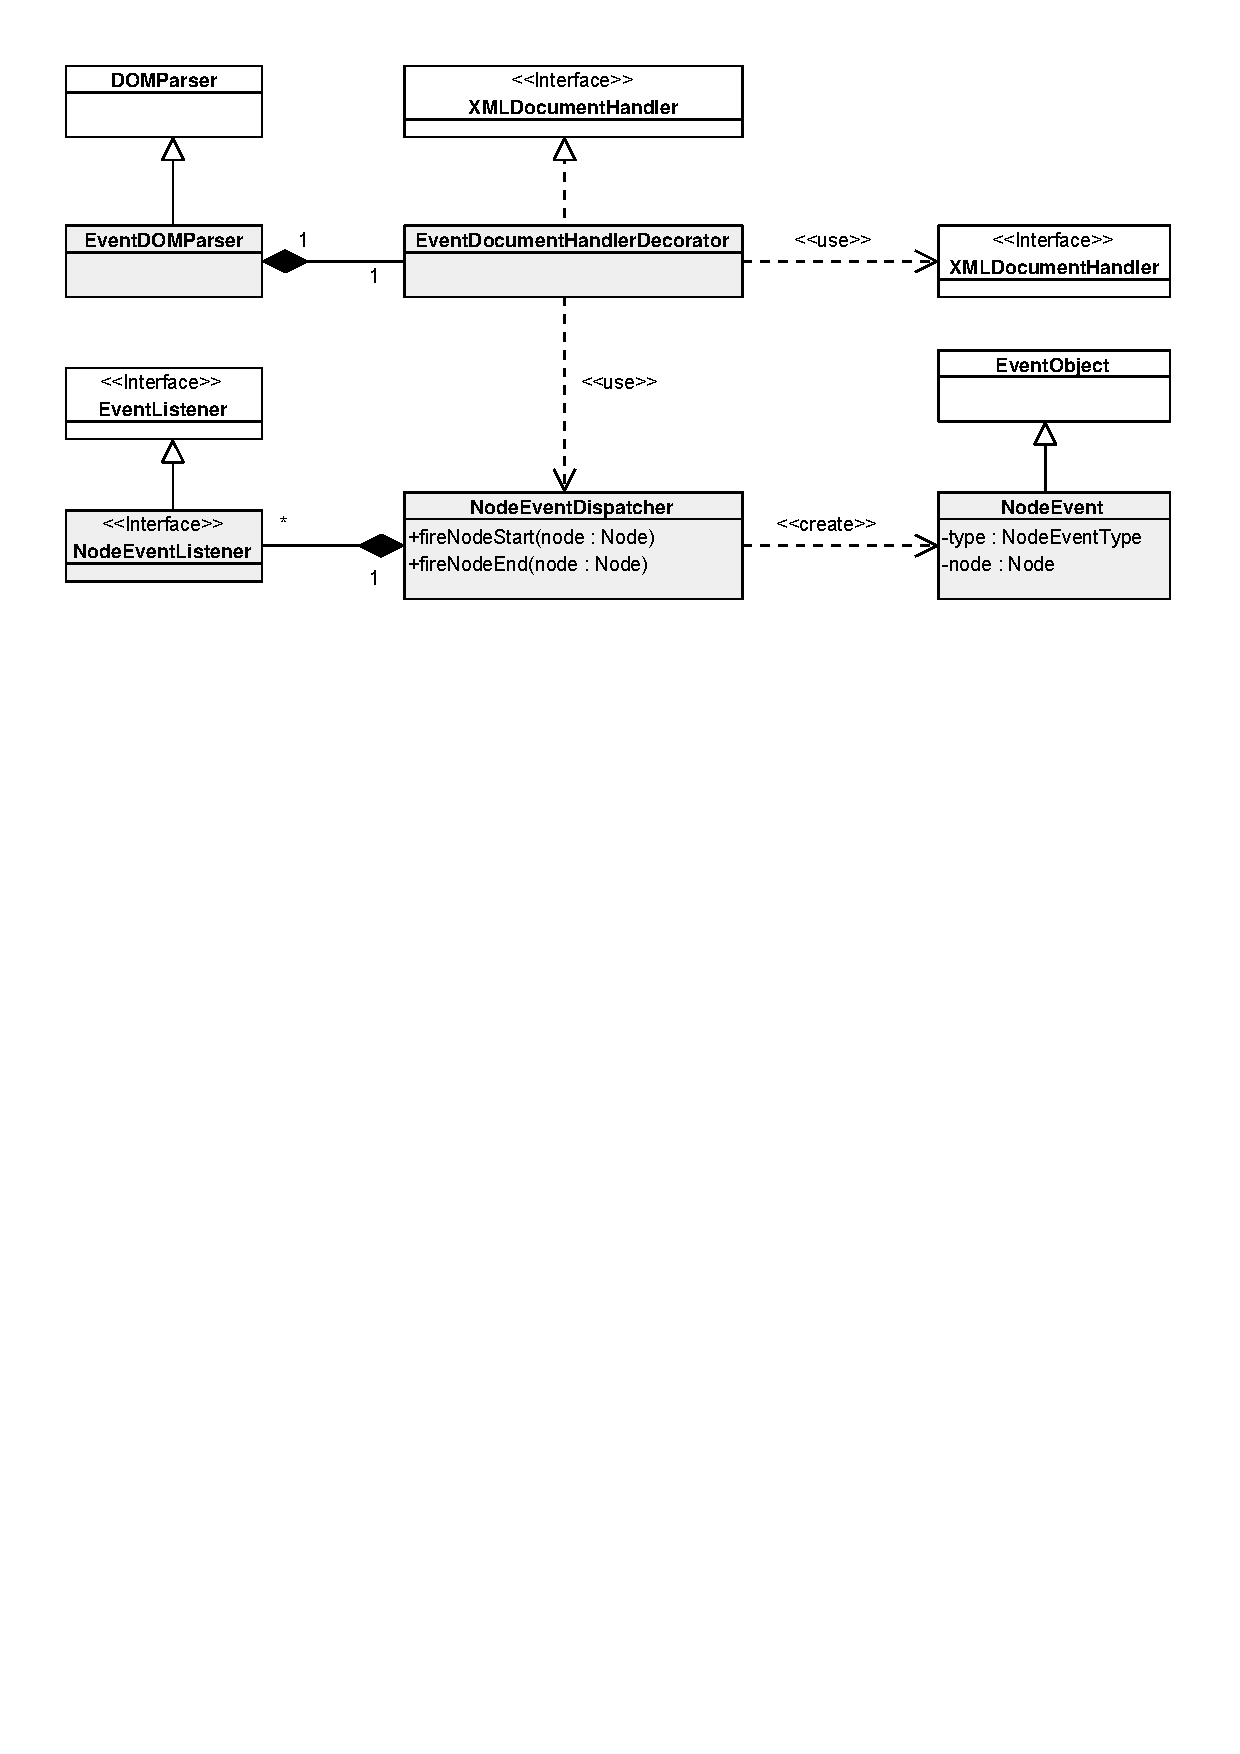
\includegraphics{fig/org-fit-cssbox-jse-document.pdf}
    }
    \caption{Diagram tříd parseru dokumentu \texttt{EventDOMParser}}
    \label{Figure.EventDOMParserDesign}
  \end{center}
\end{figure}

Podle návrhu bude nutno definovat vlastní parser \texttt{EventDOMParser}, který vychází z parseru \texttt{DOMParser} knihovny NekoHTML. Tento parser bude průběžně zpracovávat vstupní dokument a~informovat o aktuálním stavu parsování pomocí speciálních událostí. Události budou nést informaci, zda bylo zahájeno či ukončeno parsování určitého uzlu. Pokud parsování bylo dokončeno, bude si moci naslouchající objekt vyzvednout rozparsovaný uzel. 

Knihovní třída \texttt{DOMParser} využívá pro vytváření dokumentu implementované rozhraní \texttt{XMLDocumentHandler}, které obsahuje obslužné metody informující o stavu parsování. V~rámci těchto obslužných metod dochází k vytváření jednotlivých uzlů dokumentu a~konstruování výsledného stromu dokumentu. Současnou implementaci objektu, který zajišťuje konstrukci stromu dokumentu lze získat z konfigurace parseru.

Odchytávání událostí během parsování bude umožněno přenastavením aktuální implementace instance třídy \texttt{XMLDocumenthandler} v~konfiguraci parseru \texttt{DOMParser}. Naším cílem bude v~rámci volání obslužných metod zavolat i naši vlastní událost. Abychom ovšem nemuseli předefinovat celou funkčnost konstrukce dokumentu, budeme využívat starý knihovní \texttt{XMLDocumentHandler} získaný z konfigurace. Upravený \texttt{EventXMLDocumentHandler} bude knihovní handler pouze dekorovat a~zajišťovat propagaci některých události výše do třídy \texttt{EventDOMParser}. 

Aby byl návrh kompletní, byla navržena i třída \texttt{NodeEventDispatcher} vykonávající události \texttt{NodeEvent}. Všichni zájemci o naslouchání událostí si budou muset zaregistrovat naslouchající objekt ve třídě \texttt{EventDOMParser}, který dále tento objekt zaregistruje i ve třídě \texttt{NodeEventDispatcher}. Objekty odchytávající události parseru budou implementovat rozhraní \texttt{NodeEventListener} vycházející ze standardního rozhraní Javy \texttt{EventListener}.

\section{Podpora skriptování v~projektu SwingBox}
\label{Chapter.Design.ScriptsInSwingBox}

Jak bylo popsáno v~kapitole \ref{Chapter.DependenciesAnalysis.SwingBox}, projekt SwingBox umožňuje zobrazovat a~procházet webové stránky. Pro přidání podpory skriptování do tohoto projektu (viz kapitola \ref{Chapter.Design.SwingBoxIntegration}) bude nutno definovat vlastní třídu \texttt{CSSBoxAnalyzer}. SwingBox používá tuto třídu pro parsování vstupního dokumentu a~převod dokumentu na vykreslovaný \texttt{ElementBox}.   

\begin{figure}[H]
  \begin{center}
    \scalebox{0.75}{
      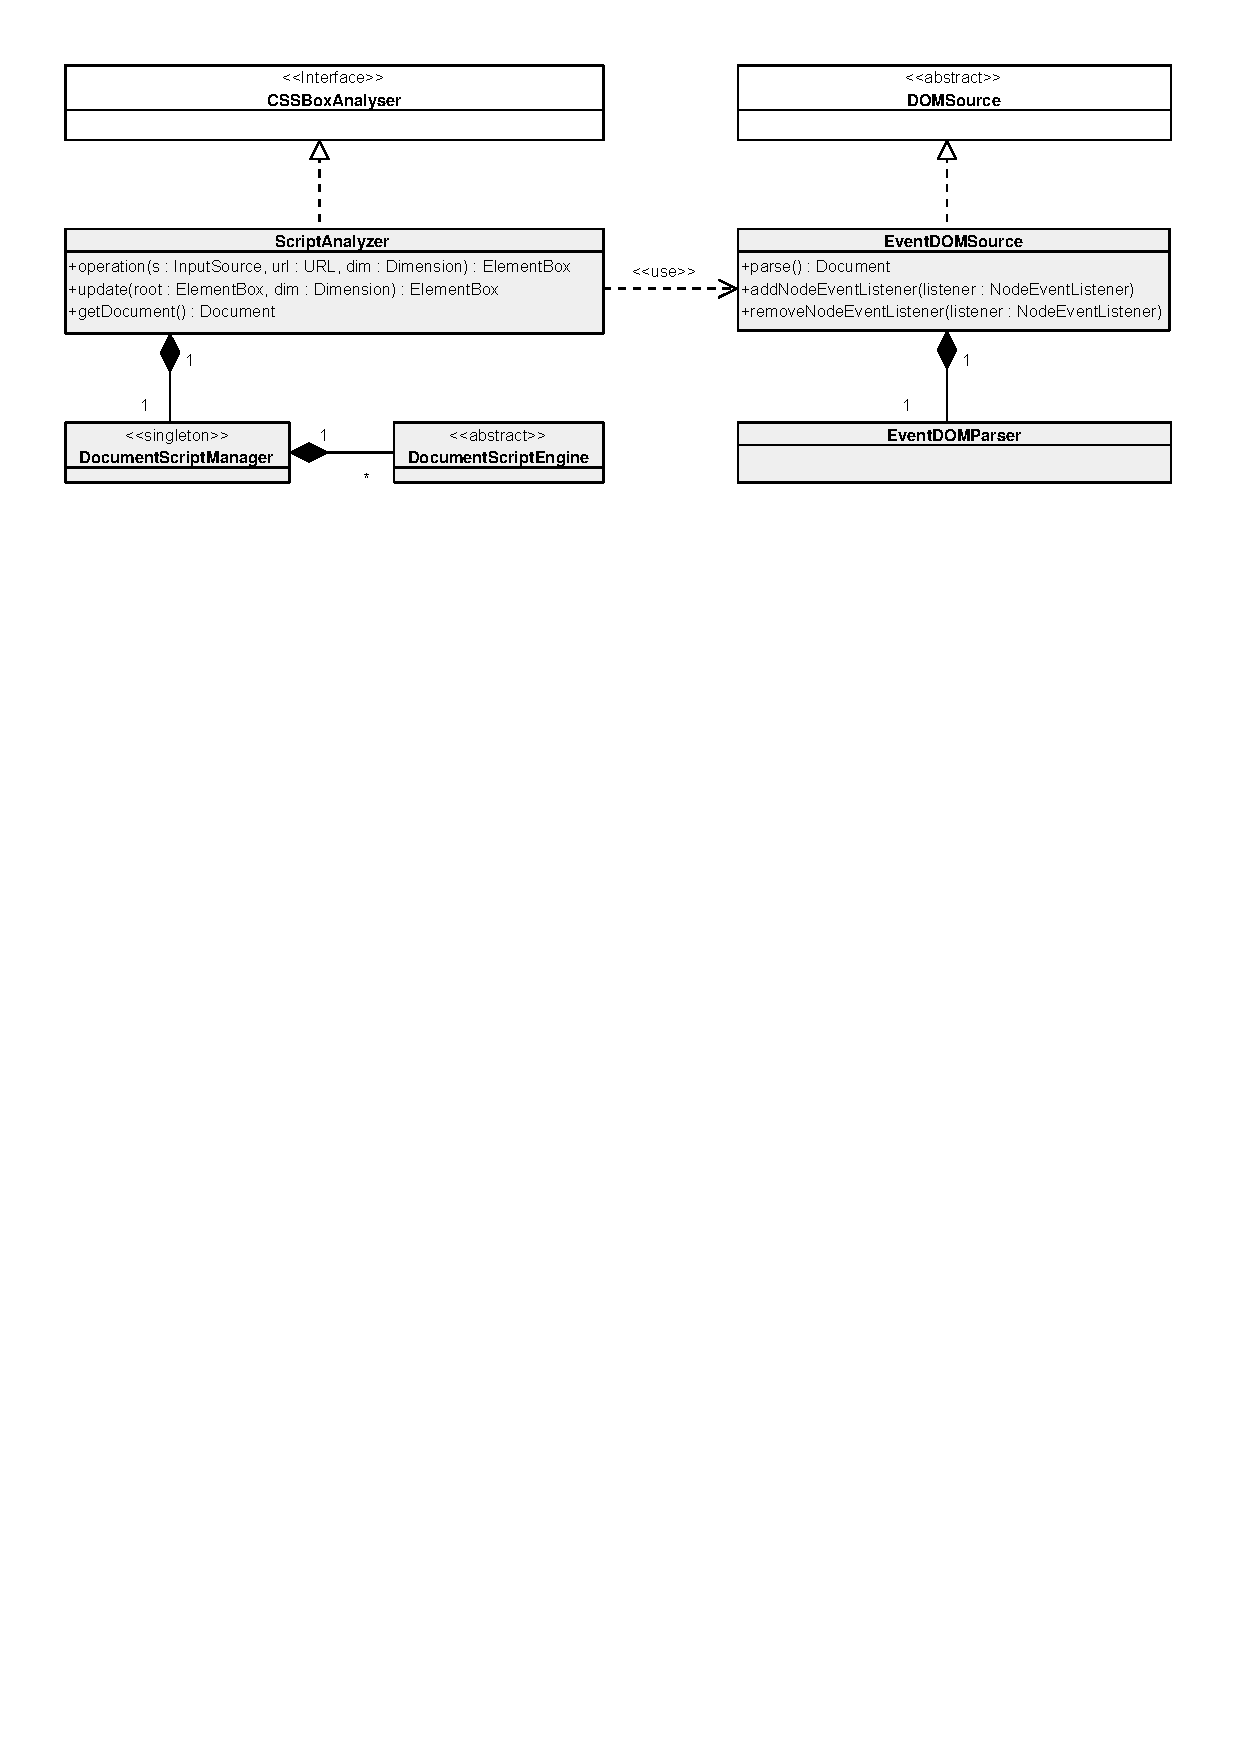
\includegraphics{fig/org-fit-cssbox-jse-util.pdf}
    }
    \caption{Diagram tříd znázorňující podporu JavaScriptu v~projektu SwingBox}
    \label{Figure.ScriptsInSwingBoxDesign}
  \end{center}
\end{figure}

Projekt \texttt{CSSBox} definuje pro zdroj dokumentu třídu \texttt{DocumentSource}, pro čtení dokumentu ze zdroje dokumentu třídu \texttt{DOMSource}. Abychom jsme se drželi zavedené praktiky pro čtení dokumentu s událostmi, v~návrhu definujeme třídu \texttt{EventDOMSource}, která pouze vnitřně používá v~kapitole \ref{Chapter.Design.ScriptsInHTML} popsaný \texttt{EventDOMParser}. 

Největší roli při invokaci skriptu hraje v~návrhu \texttt{ScriptAnalyzer}, který má u událostního parseru zaregistrovaný vlastní \texttt{EventNodeListener}. Při příchodu události o zpracování elementu \texttt{<script>}, přečte \texttt{ScriptAnalyzer} skript v~jeho těle, případně načte skript z URL adresy uvedené v~\texttt{src} atributu. Pokud skript neobsahoval atribut \texttt{defer}, tak se dále nechá ihned vykonávat ve stroji \texttt{DocumentScriptEngine}. Stroj, který má být použit pro aktuální skript je získán z instance třídy \texttt{DocumentScriptManager} na základě atributu \texttt{type} elementu \texttt{<script>}, nebo z výchozího uvedeného stroje v~\texttt{<meta>} značce (viz kapitola \ref{Chapter.DependenciesAnalysis.ScriptsInHTML}).

\begin{figure}[H]
  \begin{center}
    \scalebox{0.55}{
      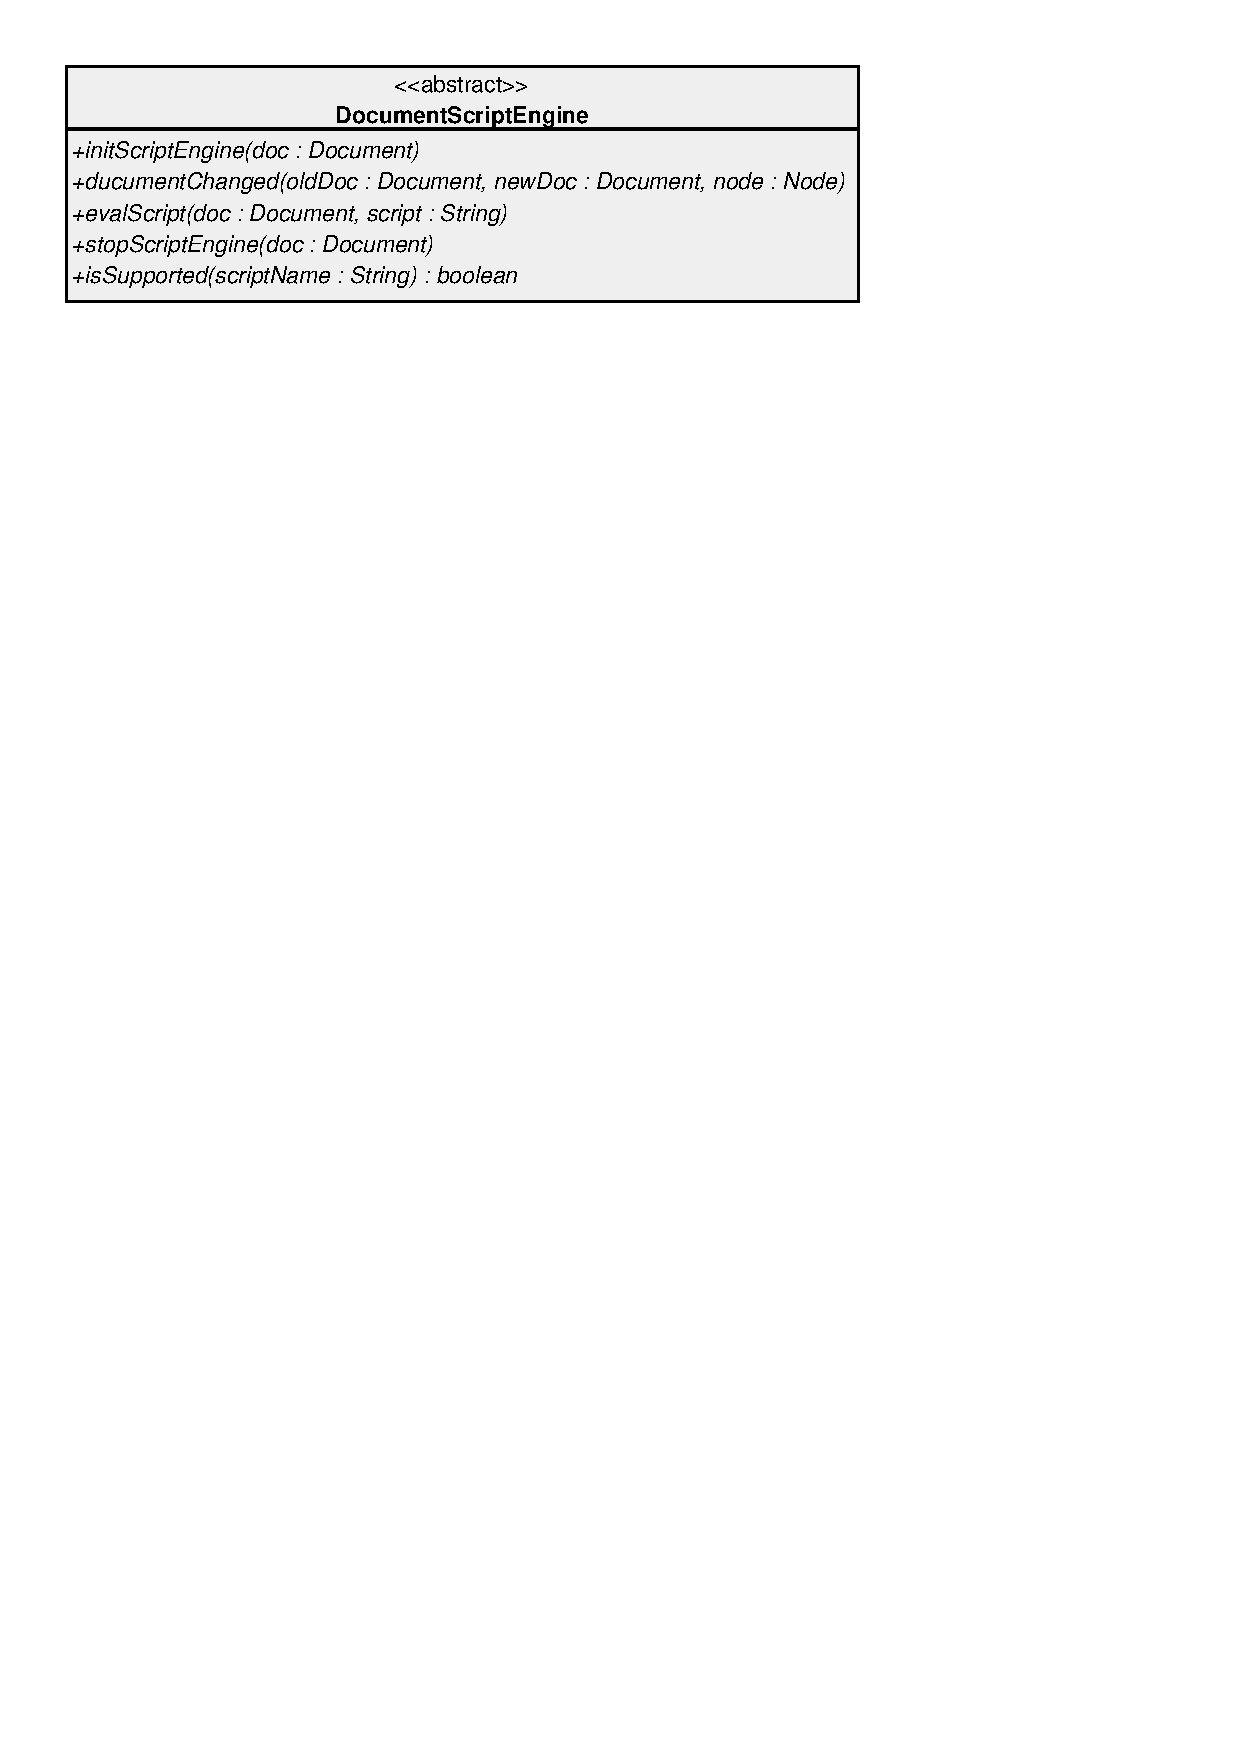
\includegraphics{fig/javascsript-engine.pdf}
    }
    \caption{Diagram abstraktní třídy \texttt{DocumentScriptEngine}}
    \label{Figure.DocumentScriptEngineDesign}
  \end{center}
\end{figure}

Pokud je skript vykováván poprvé v~rámci uvedeného dokumentu, tak dojde u třídy \texttt{DocumentScriptEngine} (obrázek \ref{Figure.DocumentScriptEngineDesign}) i k zavolání metody \texttt{initScriptEngine()}, která vytvoří globální scope pro vykonávání skriptů. V~globální scopu jsou poté vykonávány všechny skripty na stránce. Skriptovací stroj uchovává jednotlivé zaregistrované dokumenty a~jejich vykonávací globální scopy dokud není webová stránka přenačtena a~dokument není změněn. O zničení dokumentu bude stroj informován metodou \texttt{stopScriptEngine()}.

\section{Injektování objektů do hlavního scopu}
\label{Chapter.Design.GlobalScopeInjections}

Během implementace podpory klientského JavaScriptu do projektu CSSBox se
předpokládá vytvoření velkého množství tříd, které budou implementovat
jednotlivé aspekty JavaScriptu pro prohlížeč. Předpokládá se, že vyvíjené třídy budou vyvíjeny postupně a~iterativně přidávat jednotlivé funkčnosti. Bylo by výhodné oddělit jednotlivé nové funkce a~odstranit potřebu přímého zásahu do třídy \texttt{DocumentScriptEngine} s příchodem nového rozšíření.

\begin{figure}[H]
  \begin{center}
    \scalebox{0.75}{
      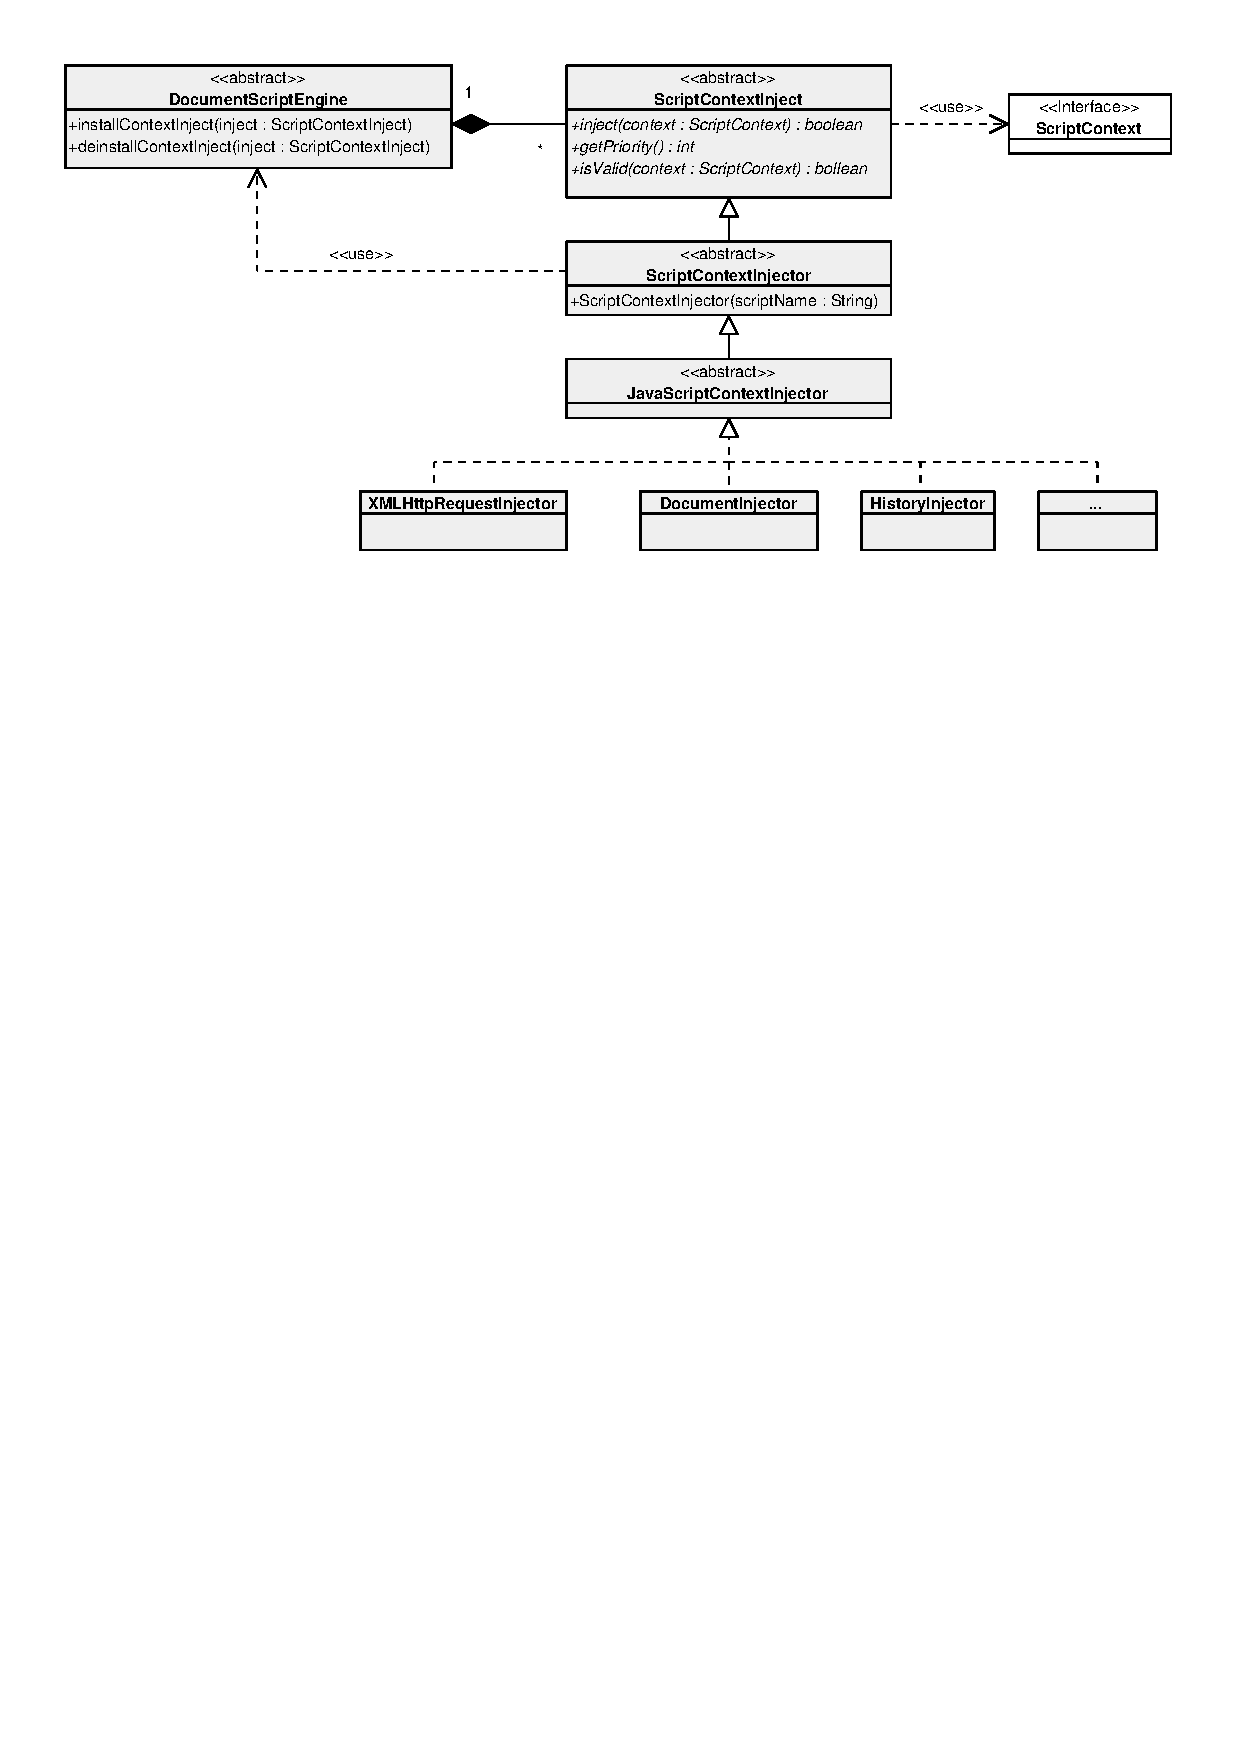
\includegraphics{fig/org-fit-cssbox-jse-script-inject.pdf}
    }
    \caption{Diagram tříd znázorňující podporu injektování rozšíření JavaScriptu}
    \label{Figure.GlobalScopeInjectionsDesign}
  \end{center}
\end{figure}

K separaci nových implementovaných vlastností JavaScriptu byla navržena technika injekce funkčnosti do vytvořeného kontextu (obrázek \ref{Figure.GlobalScopeInjectionsDesign}). Pro přidání nové funkčnosti do globálního scopu kontextu bude nutno implementovat abstraktní třídu \texttt{ScriptContextInject}. Samotnou injekci do globálního scopu bude provádět metoda \texttt{inject()}. Aby skriptovací stroj věděl, jaká rozšíření má injektovat do svého scopu, měla by být jednotlivá rozšíření registrována u skriptovacího stroje metodou \texttt{installContextInject()}. Injekce bude prováděna vždy po vyhodnocení některého skriptu, nebo po inicializování nového dokumentu. Pořadí jednotlivých injekcí bude v~základní implementaci určovat metoda \texttt{getPriority()}. Zda je injekce validní, tudíž proveditelná, bude získáváno metodou \texttt{isValid()}. Příkladem, kdy injekce by byla neproveditelná, by mohla být např. situace, kdy není ještě dokument úplně načten a~některé rozšíření by záviselo právě na existenci dokumentu.

Neustálá instalace nové injekce rozšíření do skriptovacího stroje s příchodem nového rozšíření by se postupem času nejevila jako dobré řešení. Bylo by výhodné, aby s novým rozšířením došlo i k automatické instalaci tohoto rozšíření do skriptovacího stroje, tzn., abychom dosáhli obrácení řízení -- IoC (Inversion of Control). Pro tento účel byla navržena třída \texttt{ScriptContextInjector}, která kromě metod samotné injekce bude provádět i registraci rozšíření v~odpovídajícím skriptovacím stroji. Bude-li to implementačně vhodné, k získání reference registru skriptovacích strojů \texttt{DocumentScriptManager} z objektů ScriptContextInjector se bude používat injektáž závislosti -- DI (Dependency Injection). Pro podporu DI je v~plánu použít knihovnu Google Juice. Ve třídě \texttt{ScriptContextInjector} se v~závislosti na typu skriptu vyhledá v~registru skriptovacích strojů odpovídající stroj, ve kterém proběhne registrace samotné injekce rozšíření. 

Pokud celý návrh injektování shrneme, tak automatická registrace injekce rozšíření bude probíhat v~abstraktní třídě \texttt{ScriptContextInjector}. O tom, do jakého skriptovacího stroje by se měla injekce rozšíření vložit, bude informovat pro jazyk JavaScript např. třída injektoru \texttt{JavaScriptContextInjector}. Samotná injekce rozšíření bude přitom implementována až specifickými injektory, jako jsou např. \texttt{XMLHttpRequestInjector}, \texttt{ConsoleInjector}, apod.

\section{Implementace stroje JavaScriptu podle normy JSR 223}
\label{Chapter.Design.JavaScriptEngineJSR223}

Poslední iterací v~integraci JavaScriptového stroje do projektu CSSBox by bylo přizpůsobit skriptovací stroj tak, aby splňoval bezpečnostní předpoklady pro běh v~prohlížeči. Budeme muset zabránit zejména přístupu do tříd a~balíků Javy, které nenesou žádnou funkční hodnotu pro implementaci klientského JavaScriptu. Z důvodu snazšího přechodu na jiný skriptovací stroj, např. Nashorn, by bylo výhodné, aby byl stroj implementován podle standardu JSR 223. Nashorn je vyvíjen se standardním rozhraním již od základu.

Pro tvorbu takového stroje by se nabízelo využít již existující stroj implementovaný v~Java API, který se nachází v~balíku sun.org.mozilla.JavaScript. Třídy Java API jsou ovšem finální, nebo skryty, což brání jejich znovupoužití. Nezbývá nám než implementovat vlastní skriptovací stroj, který rozšiřuje základní třídu pro skriptovací stroje AbstractScriptEngine. Tento stroj bude pro implementaci samotného skriptování využívat externí knihovnu Rhino. Rozhodnutí pro dodání externí knihovny bylo učiněno z důvodu, abychom nebyli závislí na knihovně, která je dodávaná v~JDK v~balíku \texttt{sun.org.mozilla.JavaScript.internal}. Osamostatněním na implementaci JDK získáme kompletní správu nad verzí knihovny a~nebudeme muset řešit případné problémy s příchodem JDK 8, kde již Rhino zřejmě nebude ani v~rámci základní distribuce JDK.

Způsob, kterým by mohl být implementován JavaScriptový stroj s implementovanými bezpečnostními funkcemi je navržen na obrázku \ref{Figure.JavaScriptEngineJSR223Design}:

\begin{figure}[H]
  \begin{center}
    \scalebox{0.80}{
      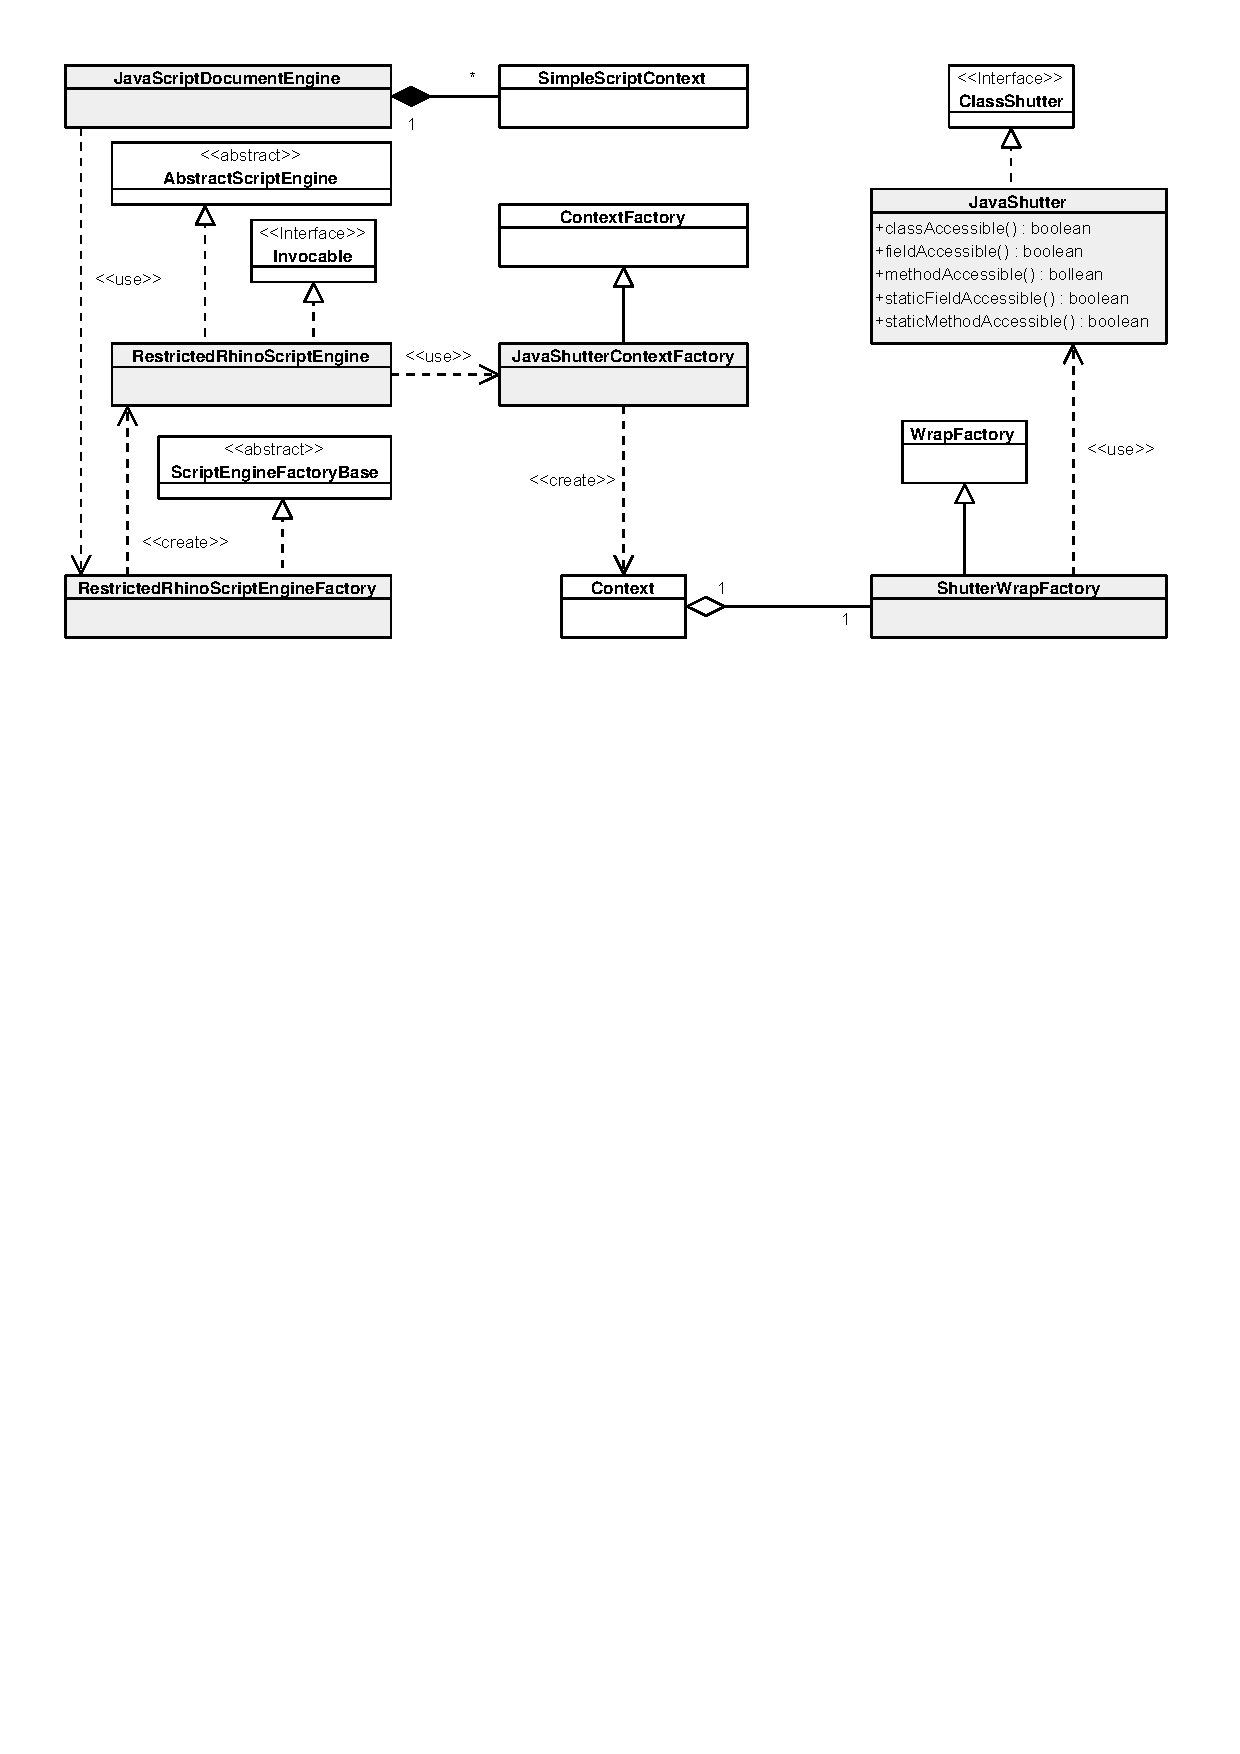
\includegraphics{fig/org-fit-cssbox-jse-script.pdf}
    }
    \caption{Diagram tříd zabezpečeného skriptavacího stroje JavaScriptu}
    \label{Figure.JavaScriptEngineJSR223Design}
  \end{center}
\end{figure}

Skriptovací stroj spravující jednotlivé načtené webové dokumenty reprezentovaný třídou \texttt{JavaScriptDocumentEngine} bude používat instanci námi upraveného skriptovacího stroje nazvaného \texttt{RestrictedRhinoScriptEngine}. Aby byla splněna specifikace JSR 223, tak bude tento stroj vytvářen pomocí továrny, která bude realizovat abstraktní třídu Java API \texttt{ScriptEngineFactoryBase}. Třída \texttt{RestrictedRhinoScriptEngine} bude muset implementovat abstraktní třídu pro všechny skriptovací stroje \texttt{AbstractScriptEngine}. Jelikož JavaScript umožňuje i volat funkce, tak bude dodatečně implementováno i rozhraní \texttt{Invocable}. 

Námi implementovaný stroj bude staticky vytvářet objekty nejvyšší úrovně a~standardní objekty JavaScriptu, které budou společné pro globální scope a~pro každé vykonávání skriptu. Staticky bude vytvořena i továrna \texttt{JavaShutterContextFactory} pro vytváření kontextu, která implementuje \texttt{ContextFactory}. Továrna je automaticky volána knihovnou Rhino pokaždé, když vstoupíme do nového kontextu metodou \texttt{Context.enter()}. Továrna kontextu bude instalovat do kontextu vlastní obalující továrnu \texttt{ShutterWrapFactory} a~objekt třídy \texttt{JavaShutter} sloužící pro omezení přístupu do jazyka Javy. Objekt omezující bezpečnost bude viditelný i z továrny pro obalování objektů Javy.

Důvodem pro předefinování továrny obalující objekty, která je volána pro každou třídu, objekt, metodu, primitivní typ Javy použitý v~kódu JavaScriptu, je právě přidání podpory rozmělnění bezpečnosti. Samotným účelem obalující továrny je dodání rozhraní \texttt{Scriptable} do objektů Javy, tak aby byly viditelné z kódu JavaScriptu. Ve vlastní implementaci továrny budeme provádět před obalením položky ověření, zda je položka viditelná. Pokud položka nemá být viditelná, tak nedojde k požadovanému obalení položky, takže položka z kódu JavaScriptu nebude viditelná.

Knihovna Rhino již obsahuje rozhraní \texttt{ClassShutter} pro zajištění bezpečnosti přístupu do Javy. Rozhraní \texttt{ClassShutter} však obsahuje pouze jednu metodu, která ověří, zda je požadovaná třída viditelná. Navrhnutá architektura na obrázku \ref{Figure.JavaScriptEngineJSR223Design} ovšem uvádí rozmělnění zabezpečení do menších položek, jako jsou povolené metody, atributy aj. Takovéto rozmělnění bude zajištěno objektem \texttt{JavaShutter}, který bude poskytovat informaci o tom, zda je přistupovaná třída, metoda, vlastnost apod. viditelná z kódu JavaScriptu. Registrace viditelných položek bude implementačně prováděna manuálně zavoláním určité metody nad objektem \texttt{JavaShutter}. Budeme mít ale i možnost nechat viditelnost odvodit automaticky podle anotace položky. Pro viditelné položky Javy zavedeme vlastní anotaci \texttt{@JSVisible}. 

Druhým bezpečnostním omezením bude omezení adaptéru zabezpečujícího implementaci rozhraní a~abstraktních tříd Javy -- \texttt{JavaAdapter}. Předpokládá se, že tato funkčnost bude kompletně zakázána.

Po vyřešení bezpečnosti budeme muset implementovat samotné propojení rozhraní Rhina a~specifikace JSR 223. Důležité bude vyřešit data binding pro kontext \texttt{ScriptContext} definovaný v~této specifikaci. Abychom měli přehled o všech proměnných, které se ve hlavním scopu nachází, budeme muset vytvořit třídu vlastního scopu. Scope (viz kapitola \ref{Chapter.JavaScriptInJavaAnalysis.Rhino.ScriptingWithRhino}) je klasický JavaScriptový objekt, ve kterém probíhá spouštění skriptu, tudíž implementuje rozhraní \texttt{Scriptable}. Rozhraní specifikuje metody pro zápis \texttt{put()} a~získání atributů \texttt{get()} z objektu. Tyto metody jsou během vykonávání skriptu náležitě volány. Zpětného volání metod využijeme k navázání atributů do objektu \texttt{Bindings} a~nebo získání atributů z objektu \texttt{Bindings}. 

Výše popsané praktiky jsou dostatečné pro vytvoření jednoduchého stroje, který vychází ze specifikace JSR 223.  Po zavolání vykonání skriptu metodou \texttt{eval()}, bude pracovat stroj tak, jak je popsáno v~následujících krocích:  

\begin{enumerate}
  \item	Vytvoří se nový kontext zavoláním \texttt{Context.enter()}, v~rámci něhož dojde i k zavolání metody \texttt{makeContext()} třídy \texttt{JavaShutterContextFactory};
  \item	Vytvoří se nový hlavní scope, který bude nastavovat a~číst \texttt{Bindings} objekt;
  \item	Do hlavního scopu se vloží standardní a~globální objekty, které budou společné pro všechny skripty. Vložení proběhne nastavením prototypu hlavního scopu;
  \item	Spustí se skript nad vytvořeným kontextem a~hlavním scopem.
\end{enumerate}

\section{Integrace podpory JavaScriptu do SwingBoxu}
\label{Chapter.Design.SwingBoxIntegration}

Všechny potřebné náležitosti pro zařazení podpory JavaScriptu do projektu CSSBox byly již navrženy. Návrh proběhl konkrétně pro podprojekt SwingBox, který rozšiřuje výchozí  CSSBox o reakci prvků stránky na podněty příchozí od uživatele, tzn. zejména o možnost procházení webového obsahu. 

Aby bylo možné zakomponovat JavaScript do projektu SwingBox, bude nutno provést registraci vlastní \texttt{CSSBoxAnalyzer} třídy navržené v~kapitole \ref{Chapter.Design.ScriptsInSwingBox}. Kompletní konfigurace, kterou bude nutno provést pro přidání podpory JavaScriptu je znázorněna na obrázku \ref{Figure.SwingBoxIntegrationDesign}.

\begin{figure}[H]
  \begin{center}
    \scalebox{0.80}{
      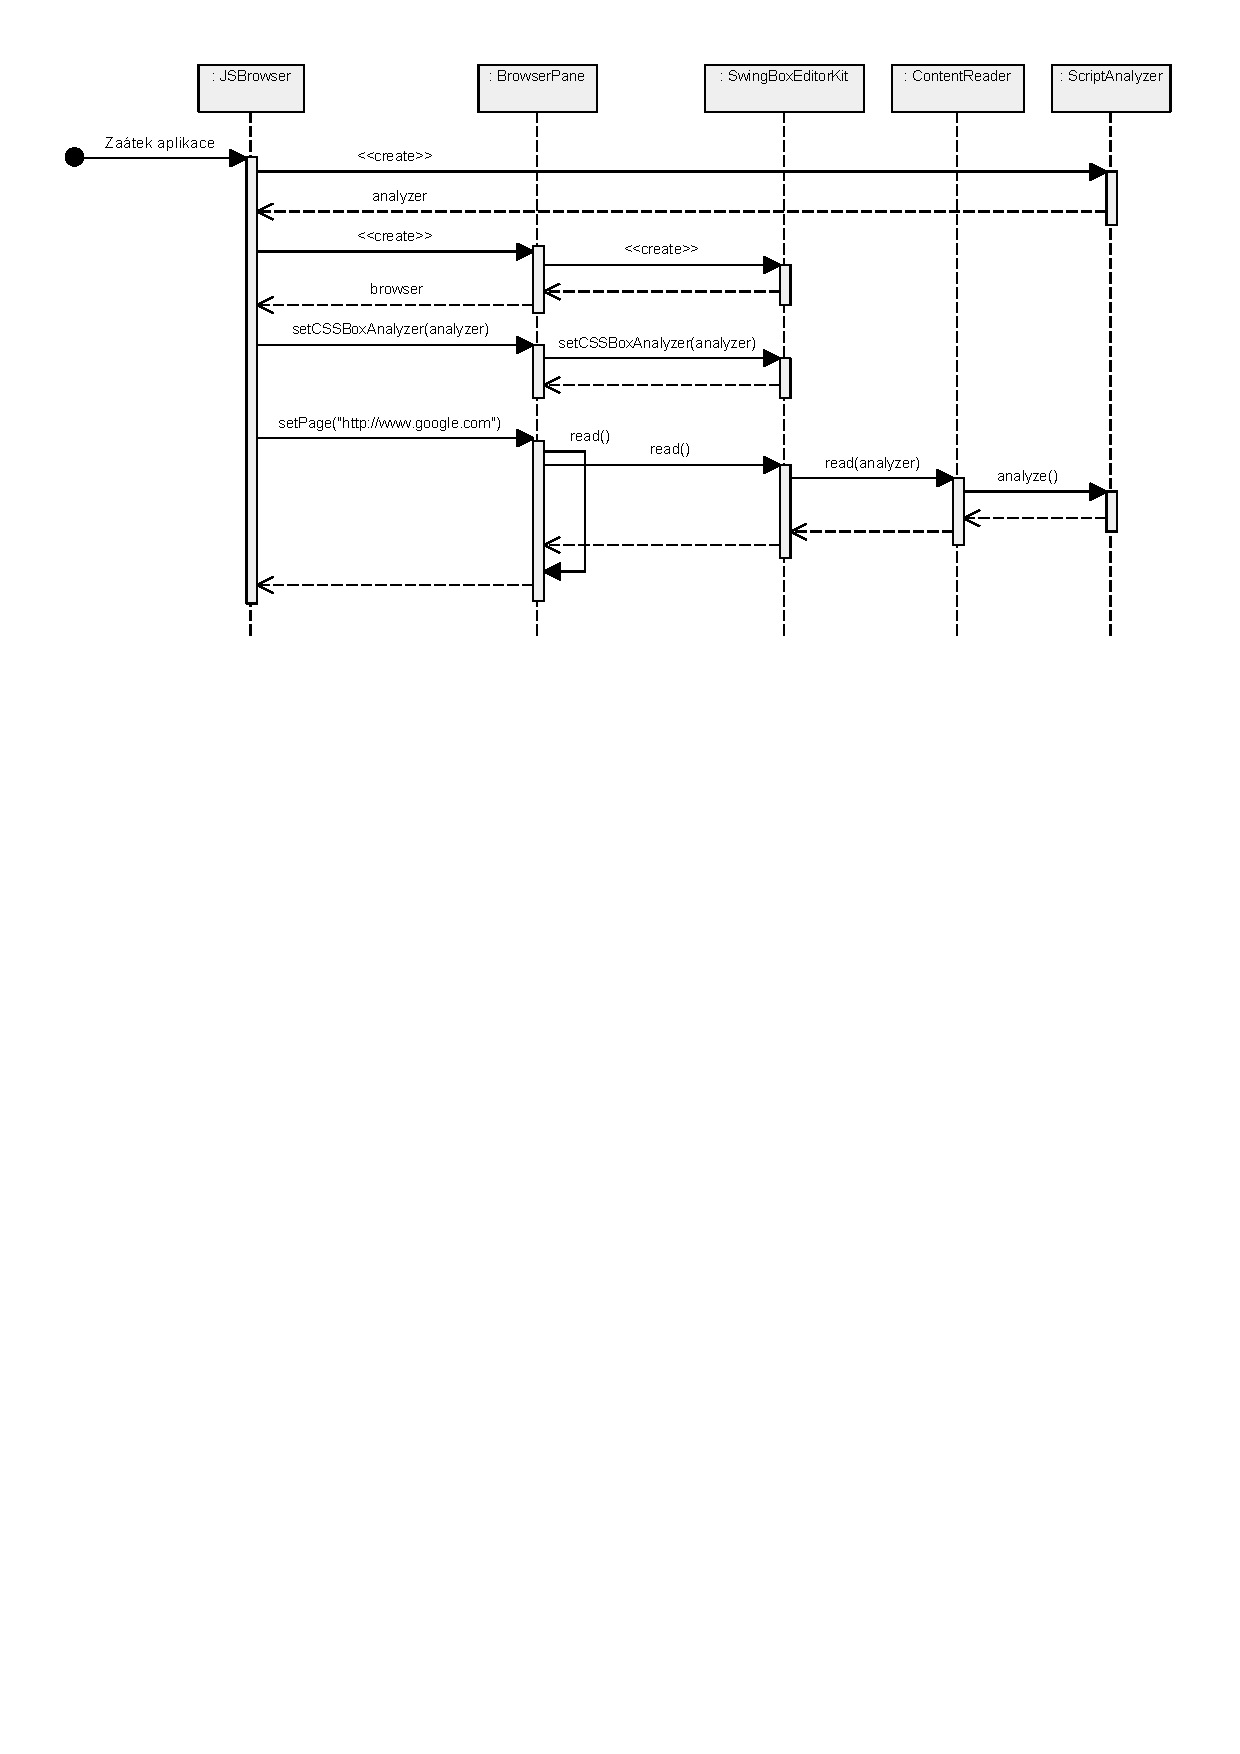
\includegraphics{fig/swingbox-integration.pdf}
    }
    \caption{Sekvenční diagram znázorňující kroky integrace JavaScriptového stroje}
    \label{Figure.SwingBoxIntegrationDesign}
  \end{center}
\end{figure}

Z uvedeného diagramu je patrné, že pouhá jedna registrace vlastního vyhodnocovače dokumentu \texttt{ScriptAnalyzer} bude pro přidání podpory JavaScriptu dostačující. Projekt SwingBox zejména implementuje vlastní zobrazovací plochu pro webové stránky \texttt{BrowserPane}. Zobrazovací plochu využijeme ve finální čísti projektu pro tvorbu jednoduchého webového prohlížeče a~znázornění funkčnosti skriptování v~HTML dokumentech. Třída pro zobrazování obsahu HTML stránky využívá pro veškeré čtení nového dokumentu webové stránky třídu \texttt{SwingBoxEditrKit}, která následně volá \texttt{ContentReader}, jenž je přímo spjat s~aktuálně zaregistrovaným \texttt{CSSBoxAnalyzer}. Definicí vlastní třídy \texttt{ScriptAnalyzer} získáme plnou kontrolu nad zpracovávaným dokumentem a~možnost provádění skriptů v~HTML dokumentu. 

\chapter{Implementace}
\label{Chapter.Implementation}

Následující kapitola pojednává o realizaci rozšíření projektu CSSBox o možnost provádění skriptů v~(X)HTML dokumentech navrženém v~kapitole \ref{Chapter.Design}. Výstupem realizace je volitelné rozšíření knihovny CSSBox v podobě knihovny. Návod na kompilaci knihovny lze nalézt v příloze \ref{Annex.manual}. Popis implementace, kterým se tato kapitola bude zabývat, je zaměřen na uvedení nejzákladnějších tříd, metod či funkcí, které implementují nejdůležitější části výsledné knihovny. Podrobný implementační popis lze nalézt v~programových dokumentacích na přiloženém DVD v příloze \ref{Annex.dvdContent}.

Cílem implementace bylo přidat podporu pro skriptování v~(X)HTML dokumentech a~zahrnout podmnožinu aktuální specifikace klientského JavaScriptu. Aby bylo možné implementovat klientské skriptovací enginy, bylo zapotřebí vytvořit jednoduché jádro prohlížeče implementující základní aspekty procházení stránek (kapitola \ref{Chapter.Implementation.BrowsingCore}). Pro snadné přidávání nových klientských skriptovacích enginů byla vytvořena abstraktní architektura pro skriptování (kapitola \ref{Chapter.Implementation.ScriptingArchitecture}), ze které vychází i JavaScriptový klientský engine (kapitola \ref{Chapter.Implementation.JavaScriptEngine}).

Implementace této práce se nachází v~podbalících hlavního balíku projektu ScriptBox pojmenovaném \texttt{org.fit.cssbox.scriptbox}.  Názvy tříd, které tyto podbalíky obsahují, nebudou v~této kapitole z důvodu zjednodušení a~přehlednosti plně kvalifikovány. Stručné popisy jednotlivých balíků jsou v~příloze \ref{Annex.packageDescription}.

\vspace{-0.5em}

\section{Jádro prohlížeče a~jeho rozhraní}
\label{Chapter.Implementation.BrowsingCore}

Jednotlivé implementace klientských skriptovacích enginů využívají různá rozhraní pro komunikaci s prohlížečem a~dokumentem, ve kterém jsou jejich skripty vloženy. Těmito rozhraními myslíme např. rozhraní pro objekty \texttt{Window}, \texttt{Location}, \texttt{History}, \texttt{Document} aj. Aby bylo možné poskytnout implementaci pro tyto zmíněné rozhraní, bylo nutné implementovat jednoduché jádro pro procházení HTML stránek.

V~této kapitole se budeme zabývat obecným jádrem pro procházení HTML stránek. Jelikož současná implementace probíhala primárně pro JavaScriptový engine, popíšeme také korespondující rozhraní, která jsou viditelná v~klientském JavaScriptu. Jednotlivá implementovaná rozhraní se snaží v~maximální možné míře využívat fundamentální koncept jádra prohlížeče. Samotné jádro je s těmito rozhraními provázáno jen minimálně.

V~kapitole \ref{Chapter.Implementation.BasicConcepts} nejprve definujeme základní pohled na prohlížeč jako na prohlížecí jednotky kontextu. Kapitola \ref{Chapter.Implementation.EventLoop} pojednává o událostní smyčce, která zapouzdřuje všechny úlohy prohlížeče. Navigace dokumentů a~jeho navracení procházením historie je popsáno v~kapitolách \ref{Chapter.Implementation.DocumentNavigation} a~\ref{Chapter.Implementation.TraversingHistory}. Následující kapitoly dokončují výklad a~přidávají další rozhraní, která jsou viditelná z klientského JavaScriptu. 

\subsection{Základní koncepty prohlížeče}
\label{Chapter.Implementation.BasicConcepts}

Prohlížečem budeme od této chvíle rozumět uživatelského agenta, angl. user agent, ať již bude, nebo nebude sloužit k prohlížení webu. Tento pojem bude reprezentovat instanci celého funkčního jádra, které umožňuje navigování HTML dokumentů a~jiných podporovaných zdrojů.

V~implementaci představuje uživatelského agenta třída \texttt{UserAgent}, která shromažďuje nastavení a~umožňuje jednotný přístup ke sdíleným datům. Hlavní funkcí uživatelského agenta je otevírání a~zavírání procházecích jednotek \texttt{BrowsingUnit} (obrázek \ref{Figure.UserAgentAndBrowsingUnit}), neboli jednotek, které zapouzdřují kontext na nejvyšší úrovni (okno, prohlížecí panel) pro zobrazování dokumentu. Hlavní procházecí kontext repezentuje třída \texttt{WindowBrowsingContext}.

\begin{figure}[H]
  \begin{center}
    \scalebox{0.63}{
      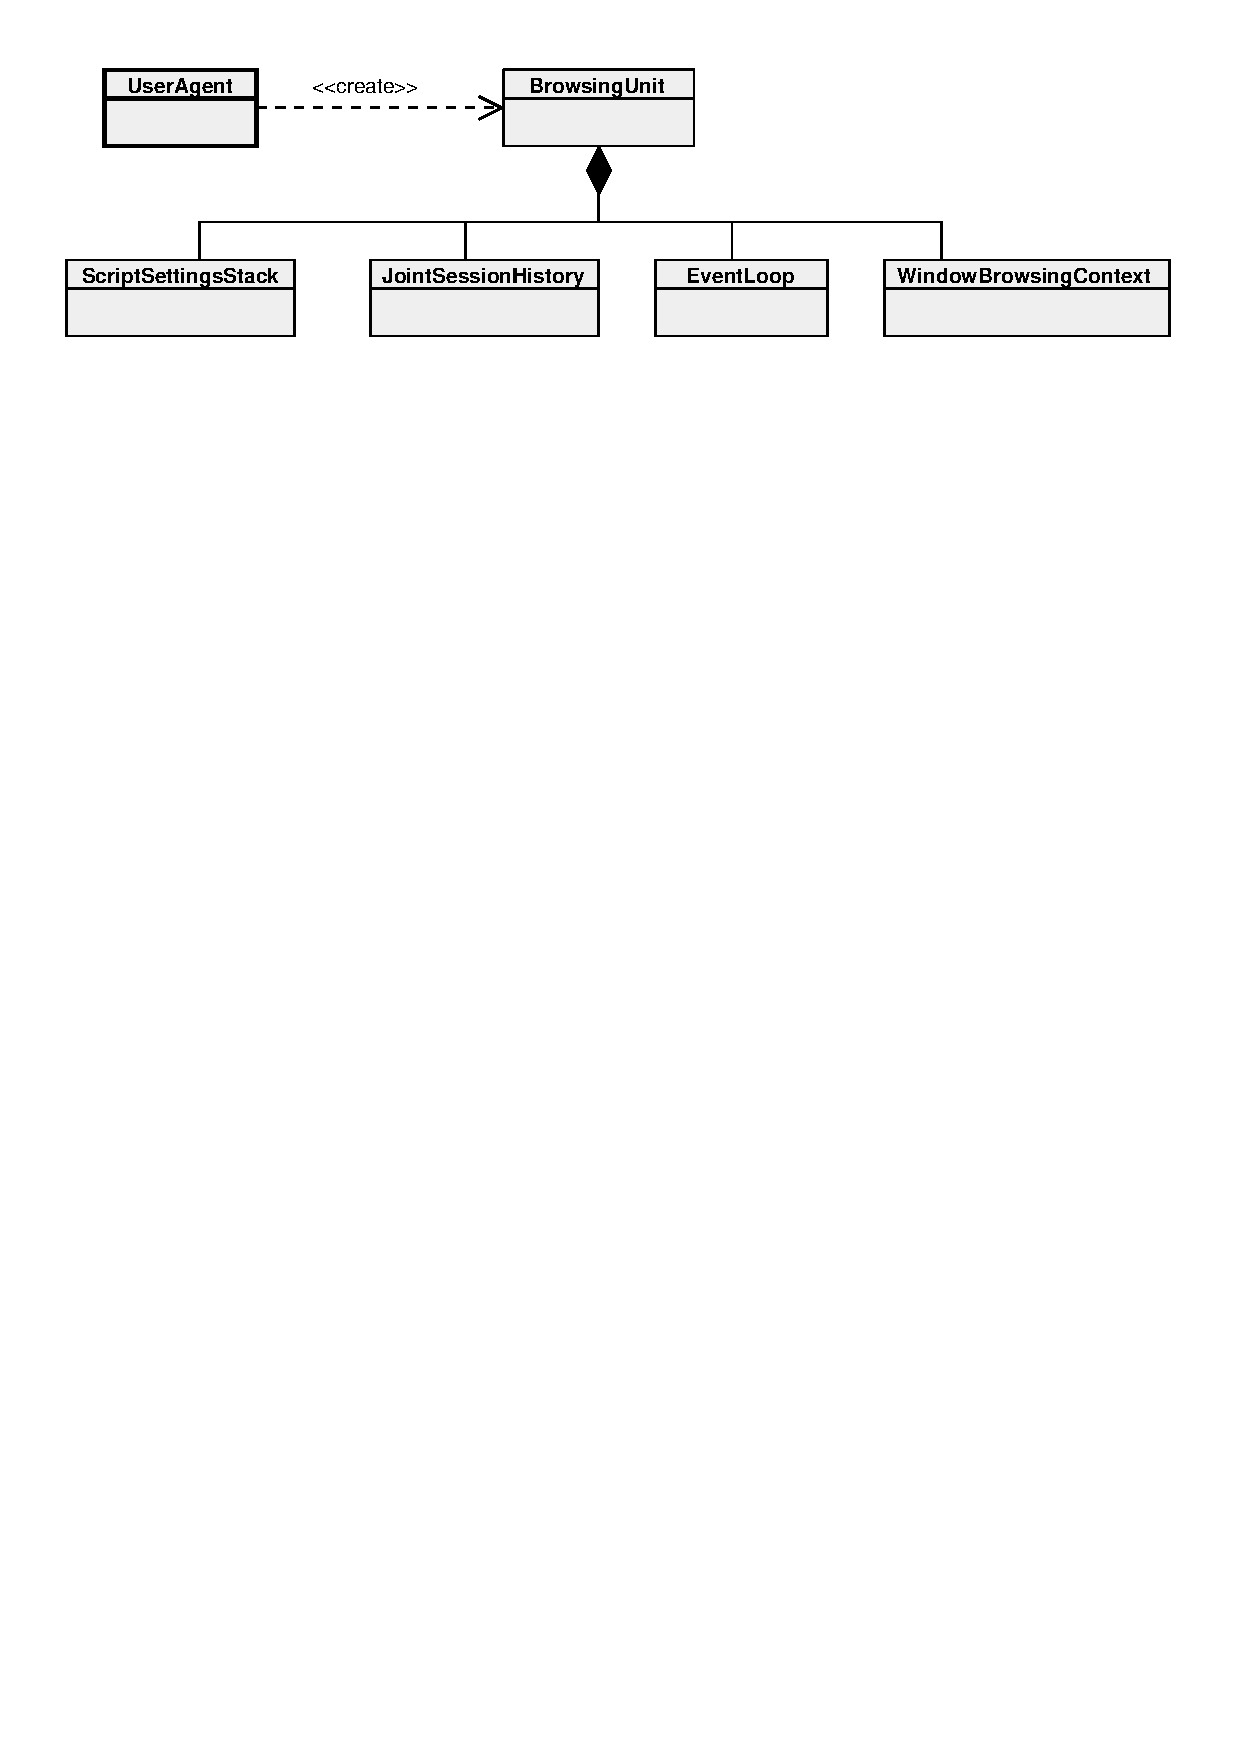
\includegraphics{fig/org-fit-cssbox-scriptbox-browser-UserAgent.pdf}
    }
    \caption{Diagram tříd procházecí jednotky vytvářené uživatelským agentem}
    \label{Figure.UserAgentAndBrowsingUnit}
  \end{center}
\end{figure}

Uvnitř jednotek je dále uchovávána reference na událostní smyčku (kapitola \ref{Chapter.Implementation.EventLoop}), historii procházení (kapitola \ref{Chapter.Implementation.TraversingHistory}) a~zásobník právě prováděných skriptů (kapitola \ref{Chapter.Implementation.ScriptInterface}), které jsou společné pro všechny obsažené procházecí kontexty. Všechny výše zmíněné objekty jsou vytvářeny v~rámci konstrukce procházecí jednotky.

Výše jsme zmínili, že procházecí jednotka vytváří procházecí kontexty. Tímto kontextem rozumíme prostředí, ve kterém jsou prezentovány dokumenty uživateli. Během navigování stránek dochází ke změně dokumentů, nikoliv~však procházecího kontextu, který je po celou životnost např. okna neměnný. Procházecí kontexty poskytují jakýsi obal nad navigovanými dokumenty a~informují o právě aktivním dokumentu.

Procházecí kontexty mohou být různě hierarchicky stromově zanořeny. Kořen stromu je umístěn vždy v~procházecí jednotce, pokud zanedbáme pomocné procházecí kontexty \texttt{AuxiliaryBrowsingContext}. Zanoření vzniká zejména díky procházecím kontextům vytvořených přes \texttt{<iframe>} značky, které mohou obsahovat zanořené dokumenty.

Pokud je uživatelským agentem agent, který obsahuje uživatelské prostředí, tak má procházecí kontext velmi blízké provázání právě na toto uživatelské prostředí, ve kterém je zobrazován dokument. Proto byl kontext zvolen i pro definici rozhraní umožňujícího základní přístup k uživatelskému rozhraní z klientských skriptů. V~kontextu se nachází rozhraní například pro navigační pole, statusový panel, posuvníky aj. Podle HTML 5 jsou tato uživatelská rozhraní viditelná skrze BarProp rozhraní . Abychom odstínili vytváření nových „schopnějších“ procházecích kontextů při každé potřebě na změnu uživatelského rozhraní, je možné tato rozhraní nastavovat v~obecných a~již implementovaných procházecích kontextech pomocí odpovídajících setterů. Jelikož základní uživatelský agent \texttt{UserAgent} žádné uživatelské prostředí nedefinuje, základní implementace procházecích kontextů neposkytuje ani kompletní implementaci BarProp rozhraní. Implementace je provedena pouze formou nekompletních metod, známých angl. pod pojmem stubs, který budeme od této chvíle v~textu dále používat.

Abstraktní třídu pro všechny procházecí kontexty představuje třída \texttt{BrowsingContext} (obrázek \ref{Figure.BrowsingContext}), která obsahuje metody pro vytváření a~hierarchickou strukturalizaci procházecích kontextů a~ostatní funkcionalitu společnou pro všechny specifické kontexty. Třída vlastní referenci na historii sezení \texttt{SessionHistory} (kapitola \ref{Chapter.Implementation.TraversingHistory}), navigační kontroler \texttt{NavigationController} (kapitola \ref{Chapter.Implementation.DocumentNavigation}) a~objekt \texttt{WindowProxy} (kapitola \ref{Chapter.Implementation.WindowInterface}).

\begin{figure}[H]
  \begin{center}
    \scalebox{0.70}{
      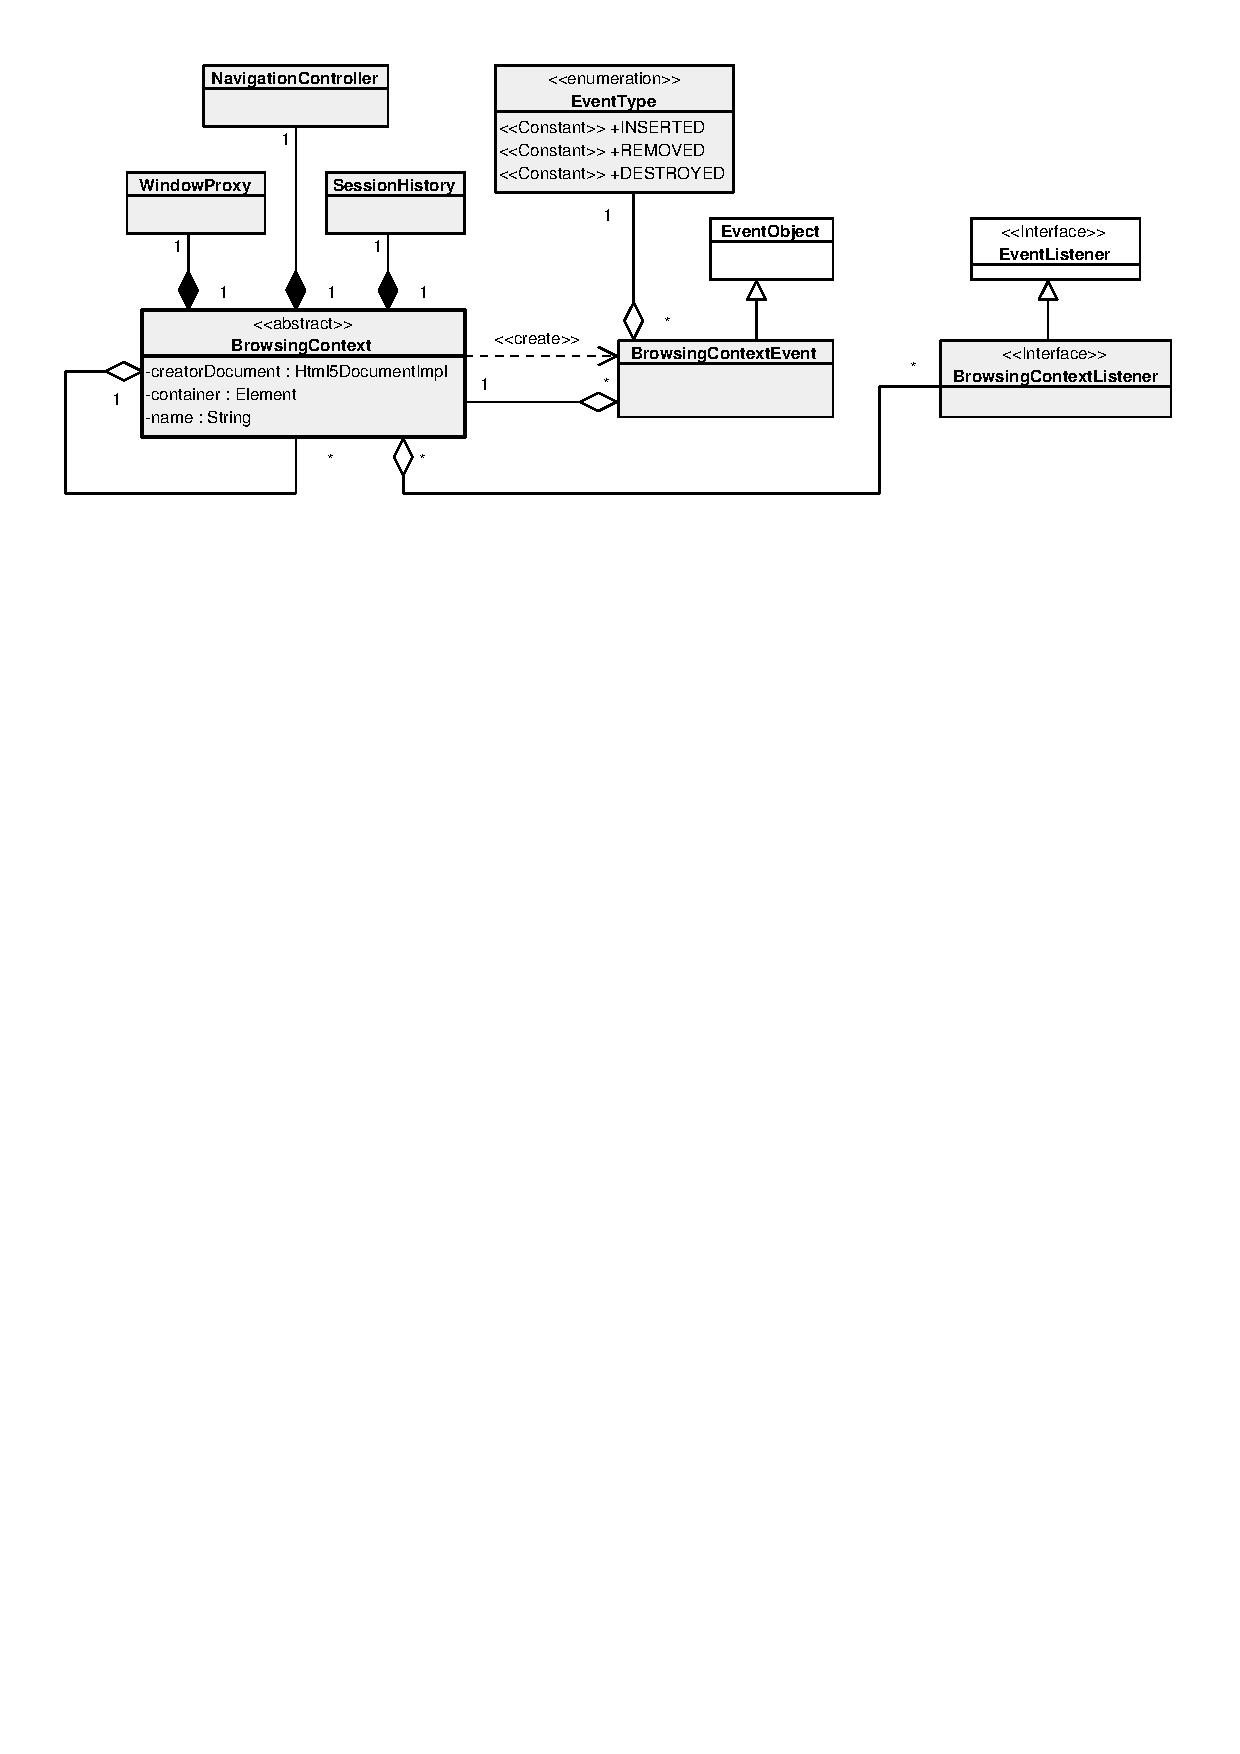
\includegraphics{fig/org-fit-cssbox-scriptbox-browser-BrowsingContext.pdf}
    }
    \caption{Diagram tříd procházecího kontextu}
    \label{Figure.BrowsingContext}
  \end{center}
\end{figure}

\noindent Nejdůležitějšími atributy třídy \texttt{BrowsingContext} jsou:

\begin{itemize}
  \item \textbf{\texttt{creatorDocument}} -- reference na dokument, který vytvořil procházecí kontext;
  \item \textbf{\texttt{container}} -- element, v~rámci něhož byl vytvořen procházecí kontext;
  \item \textbf{\texttt{name}} -- jméno procházecího kontextu.
\end{itemize}

\noindent Všechny specifické implementované procházecí kontexty jsou znázorněny na obrázku \ref{Figure.BrowsingContextsHierarchy}.

\begin{figure}[H]
  \begin{center}
    \scalebox{0.50}{
      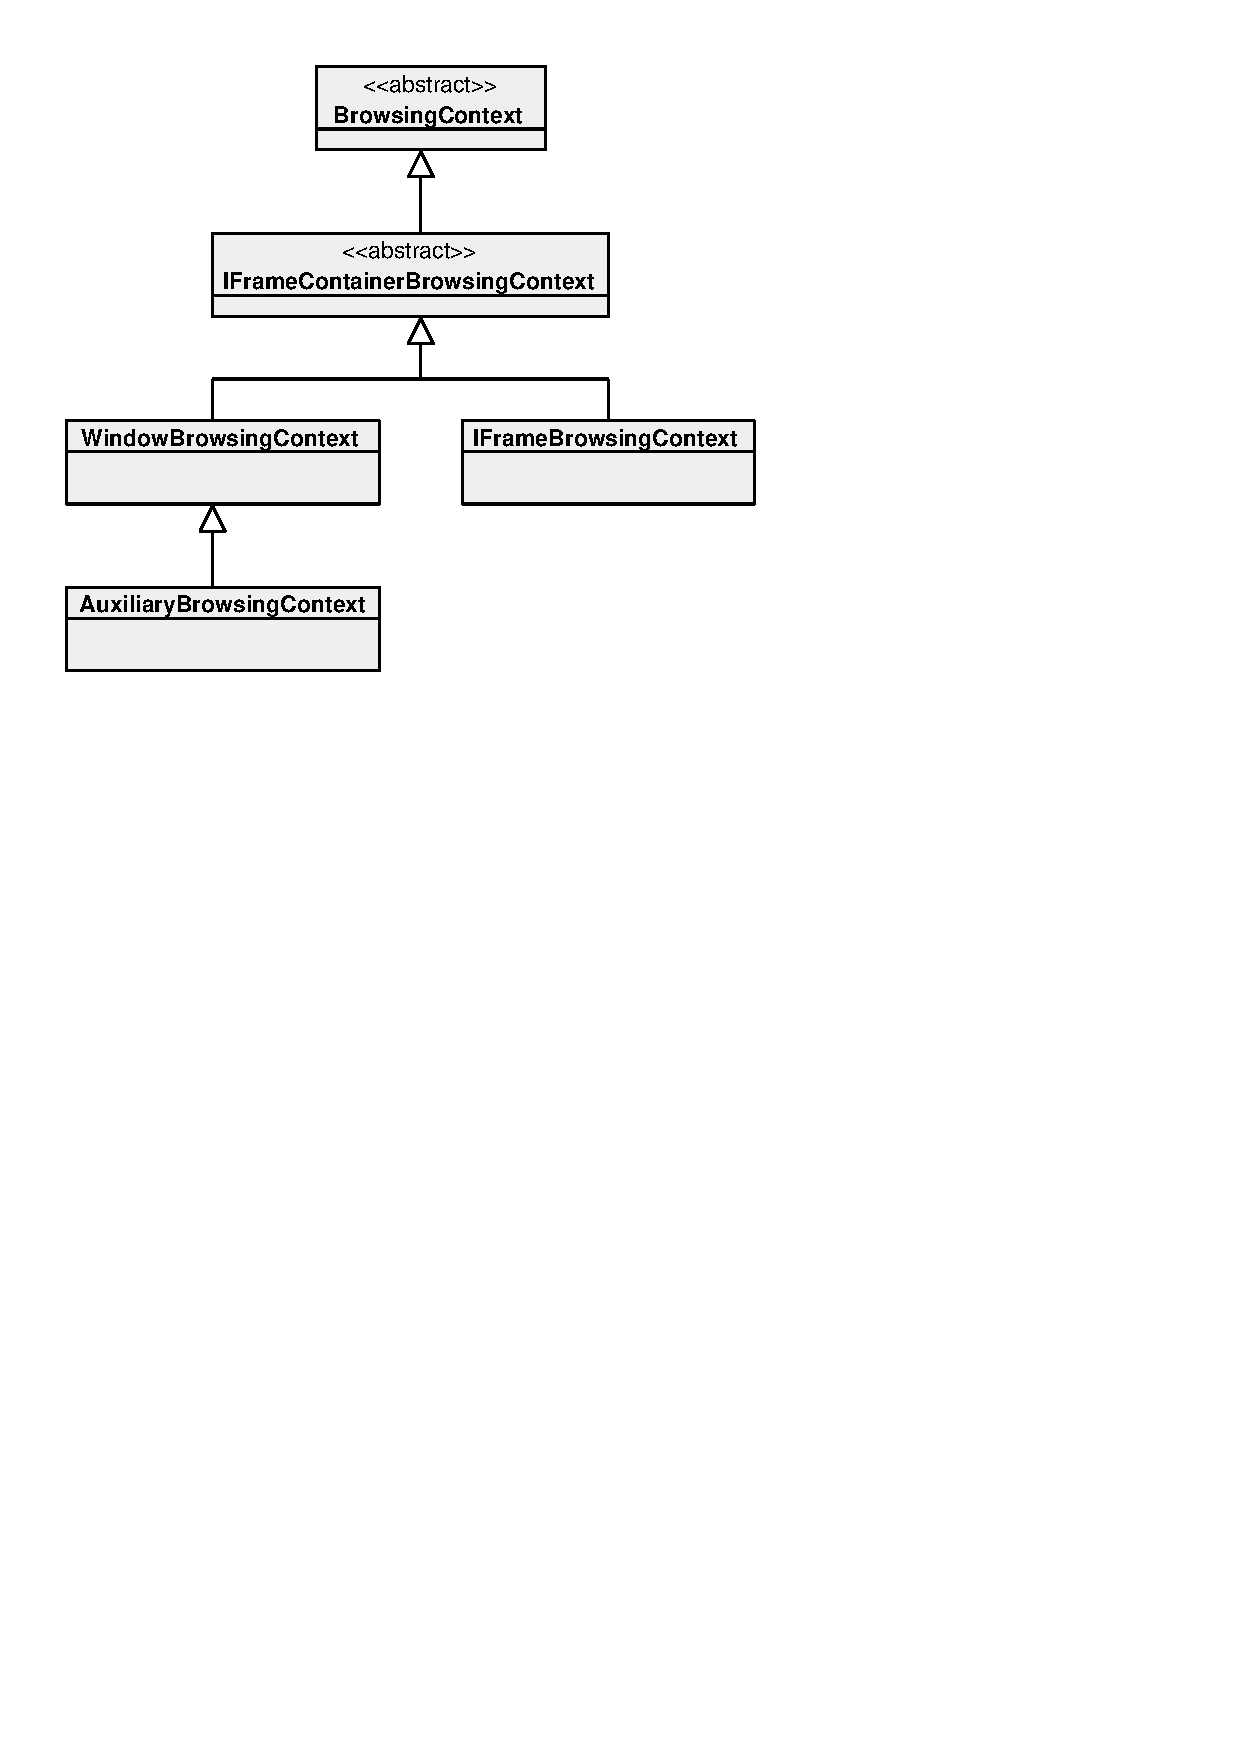
\includegraphics{fig/org-fit-cssbox-scriptbox-browser-ContextsHierarchy.pdf}
    }
    \caption{Diagram tříd hierarchie procházecích kontextů}
    \label{Figure.BrowsingContextsHierarchy}
  \end{center}
\end{figure}

Z třídy kontextu dědí další abstraktní třída \texttt{IFrameContainerBrowsingContext}, která je určena pro všechny procházecí kontexty, jenž mohou vytvářet zanořené procházecí přes značky \texttt{<iframe>}. Další třídy \texttt{WindowBrowsingContext} a~\texttt{IFrameBrowsingContext} reprezentují již konkrétní procházecí kontexty. Třída \texttt{WindowBrowsingContext} představuje kontext na nejvyšší úrovni -- tedy na úrovni okna. Druhá třída \texttt{IFrameBrowsingContext} pak plní funkci vnořeného kontextu vytvářeného uvnitř \texttt{IFrameContainerBrowsingContext} přes značku \texttt{<iframe>}. Pomocný kontext \texttt{AuxiliaryBrowsingContext} je dalším kontextem na nejvyšší s tím rozdílem, že není vytvářen procházecí jednotkou jako u kontextu okna. Kontext je naopak vytvářen libovolným specifickým kontextem, který potřebuje otevřít nové okno, vznikajícím např. navigací cíle \_blank.

V~průběhu implementace se naskytla potřeba pro získávání notifikací z procházecích kontextů při výskytu určité události, a~tak byl implementován jednoduchý observer mechanismus nad procházecími kontexty. Procházecí kontext \texttt{BrowsingContext} může vyvolat události:

\begin{itemize}
  \item \textbf{\texttt{INSERTED}} -- po vložení nového zanořeného kontextu do daného kontextu;
  \item \textbf{\texttt{REMOVED}} -- při smazání vnořeného kontext z daného kontextu;
  \item \textbf{\texttt{DESTROYED}} -- pokud je daný kontext zrušen. 
\end{itemize}

\subsection{Událostní smyčka}
\label{Chapter.Implementation.EventLoop}

Abychom mohli pokračovat ve výkladu, je zapotřebí se seznámit s událostní smyčkou, která obsluhuje úlohy uživatelského agenta. Událostní smyčka umožňuje úlohy dle potřeby mazat, různě filtrovat nebo je oddělit podle jejich typu -- zdroje úlohy. Smyčka dále sjednocuje přístup k API uživatelského agenta v~jednom vlákně, aby nedocházelo k race condition a~ulehčilo se řešení výlučných sekcí. Asynchronní žádosti na API, jako je např. navigování stránek nebo procházení historie, v~určitém čase vždy zajistí vložení nové úlohy do událostní smyčky.

V~implementaci je událostní smyčka reprezentována třídou \texttt{EventLoop} a~je vytvářena procházecí jednotkou v~rámci její konstrukce. Zjednodušený diagram tříd znázorňující funkci událostní smyčky lze vidět na následujícím obrázku \ref{Figure.EventLoop}. 

\begin{figure}[H]
  \begin{center}
    \scalebox{0.78}{
      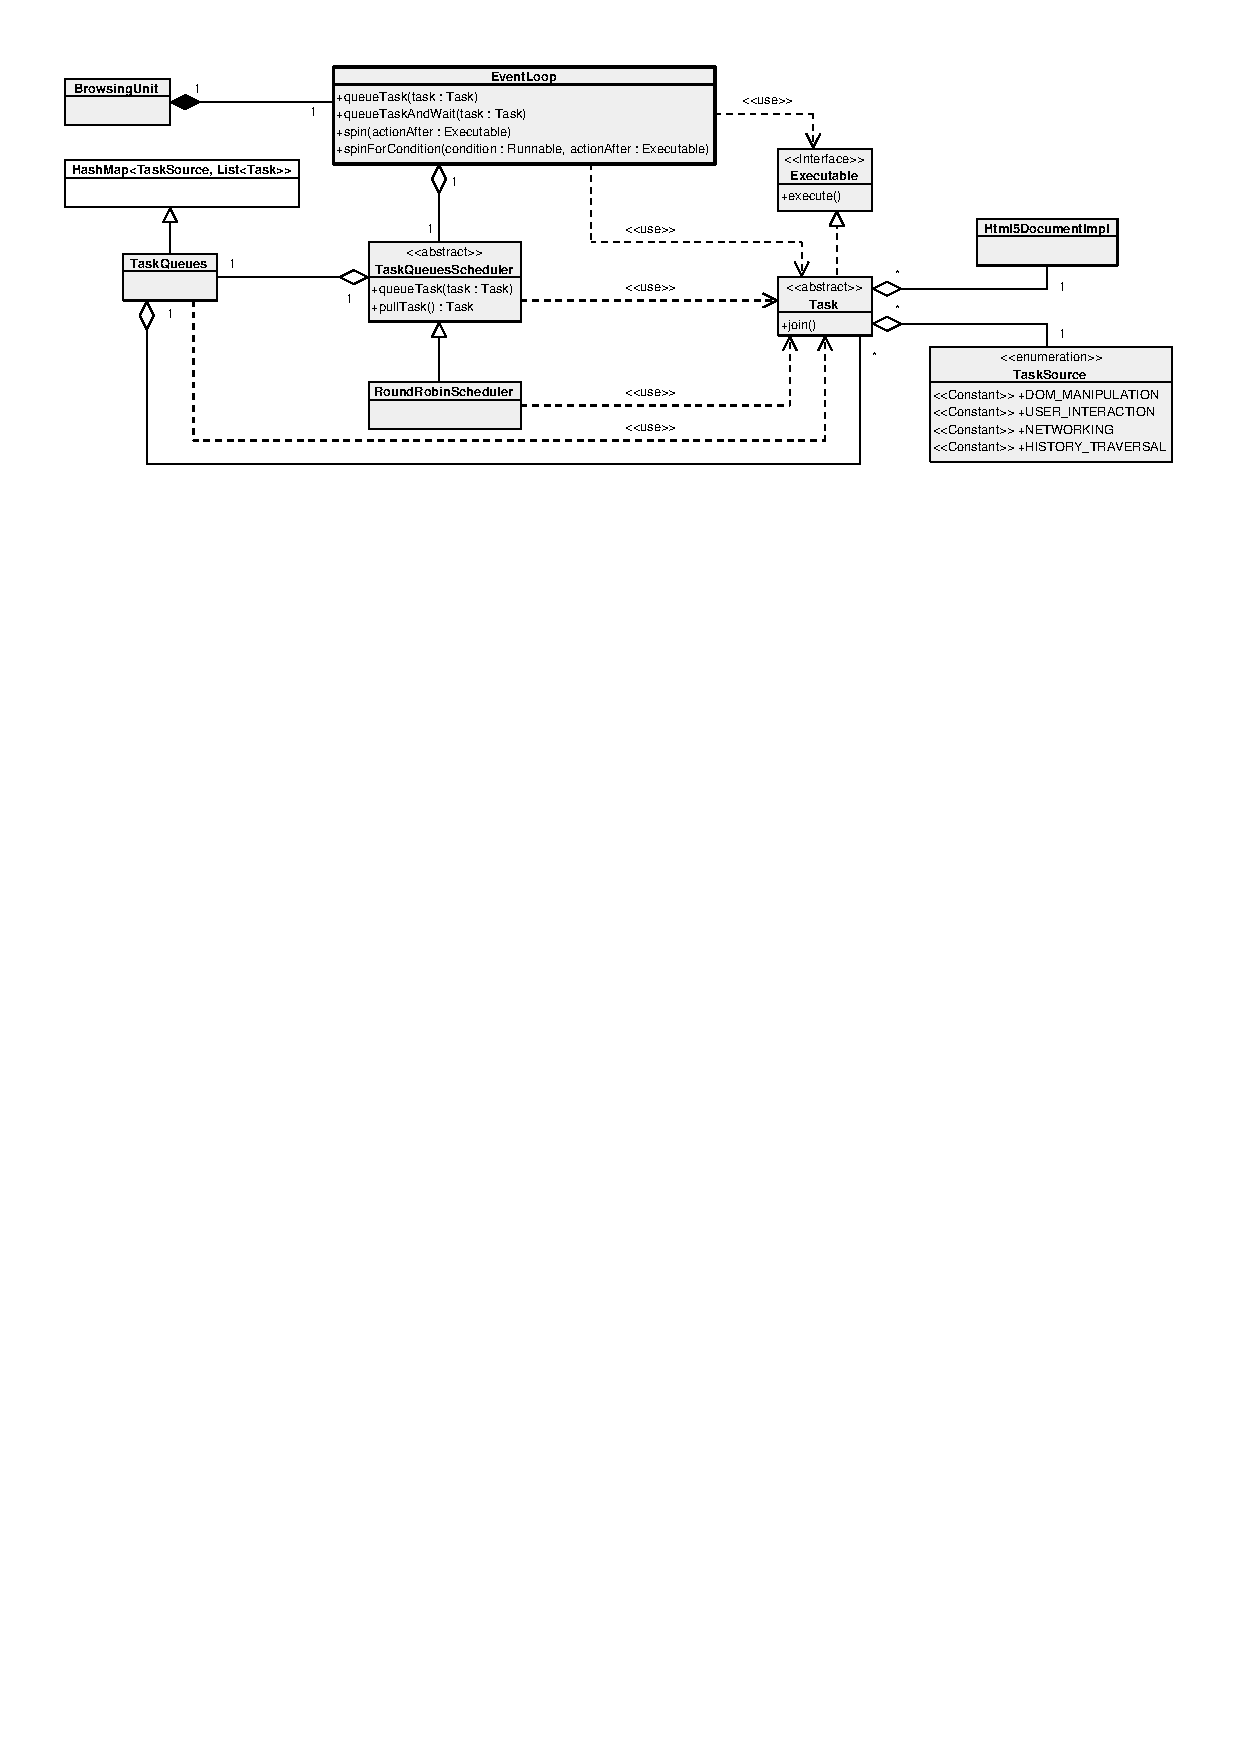
\includegraphics{fig/org-fit-cssbox-scriptbox-events-EventLoop.pdf}
    }
    \caption{Diagram tříd znázorňující událostní smyčku}
    \label{Figure.EventLoop}
  \end{center}
\end{figure}

Nejdůležitější metoda smyčky je \texttt{queueTask()}, která vkládá nové úlohy \texttt{Task} do front úloh \texttt{TaskQueues} v~závislosti na tom, o jakou frontu se jedná. Rozlišení front je docíleno zdrojem úlohy \texttt{TaskSource}. Vkládání úloh a~její vybírání zprostředkovává plánovač \texttt{TaskQueuesScheduler}.
 
Kromě operace na vkládání nových úloh obsahuje událostní smyčka různé variace metod na~filtraci a~mazání úloh. Tyto metody obsahují ve svých názvech prefixy \texttt{filter\ldots()} a~\texttt{remove\ldots()}. Při konstrukci smyčky se vytváří nové vlákno, které čeká, dokud není naplánována nová úloha plánovačem úloh. Obecně platí, že událostní smyčka je vláknově bezpečná. Pokud si přejeme pozdržet vlákno, které vložilo úlohu do front úloh, lze toho docílit metodou \texttt{queueTaskAndWait()}, která interně volá metodu \texttt{join()} nad danou úlohou. Pokud bychom použili metodu \texttt{queueTaskAndWait()} přímo z vykonávacího vlákna smyčky, došlo by k jeho zablokování. Proto je zapotřebí využít jiných technik, např. zavolání metody \texttt{spin()} poté, co je vložena nová úloha.

Metoda \texttt{spin()} a~její variace s prefixem spin zajišťují rotaci událostní smyčky. Rotací rozumíme přerušení aktuálně prováděné úlohy a~její opětovné vložení, přičemž vložení může být různě zpožděno. Základní metoda na rotaci \texttt{spin()} vkládá úlohu ihned do front úloh, zatímco metoda \texttt{spinForCondition()} čeká na splnění určité podmínky. Podmínky jsou implementovány rozhraním \texttt{Runnable}, jehož metoda \texttt{run()} je při žádosti na odložené vložení zavolána ve speciálním vlákně. Po skončení vlákna dojde teprve ke vložení úlohy do front úloh. Přerušení právě probíhající úlohy je zajištěno vyhozením kontrolované výjimky \texttt{TaskAbortedException}, která pokud není nikde odchycena, je propagována až do událostní smyčky. Smyčka po zachycení dané výjimky začne považovat právě vykonávající úlohu jako za dokončenou. Úloha, která je vložena rotací smyčky do front úloh, je kopií staré úlohy ovšem s novým vykonávacím tělem, jež je předáváno jako \texttt{actionAfter} parametr do metod pro rotace. Využití rotací událostní smyčky lze využít např. během posouvání na fragment stránky, přičemž stránka není ještě stále kompletní. V~tomto případě lze rotací zapříčinit čekání na daný fragment a~poté, co je vložen do dokumentu, vložit úlohu, která zajistí posunutí na daný fragment.

Jak víme, každá úloha musí rozšiřovat abstraktní třídu Task. Úloha musí být dále také asociována s dokumentem a~musí nést zdroj, podle kterého se rozhoduje, do jaké fronty se má úloha zařadit. Položka dokumentu v~úloze velmi často slouží k určení cíle úlohy, čehož se využívá při odstraňování úloh pro dokumenty, které vystoupily z procházecího kontextu, např. pokud došlo k navigaci na jiný dokument. 

Fronty úloh \texttt{TaskQueues} jsou rozšířením hašovací tabulky, která mapuje zdroje úloh na fronty přiřazené tomuto zdroji. Třída \texttt{TaskQueues} přidává nové metody pro intuitivnější práci s frontami úloh -- metody pro vyhledávání úloh ve frontách, jejich filtraci a~odstraňování.

Cílem plánovače úloh \texttt{TaskQueuesScheduler} bylo zajistit oddělené plánování úloh od událostní smyčky a~umožnit v~budoucnu různé implementace plánování. Tak jako událostní smyčka, má plánovač vlastní vlákno pro plánování. Přes své rozhraní přijímá nové úlohy, které vkládá do front úloh. Ve vlastním vykonávacím vlákně tyto úlohy podle plánovacího algoritmu vybírá a~vkládá je do fronty naplánovaných úloh. V~současnosti jediná implementace plánovače úloh \texttt{RoundRobinScheduler} zajišťuje rotační odebírání úloh z front úloh, přičemž pokud je některý zdroj úlohy neaktivní a~jeho fronta je prázdná, je po určitém časovém kvantu vnitřním časovačem odstraněn z pole pro rotaci.

\subsection{Stahování zdrojů}
\label{Chapter.Implementation.DownloadingResources}

Předtím než přejdeme k popisu dokumentu a~jeho parsování, popíšeme v~následující kapitole, jak je řešeno jeho stažení. Stahování bylo řešeno obecně pro různé typy komunikačních protokolů a~pro různé typy formátů obsahu. Jelikož lze stahovat různé druhy obsahu, nikoliv~pouze dokumenty, budeme se v~této kapitole bavit pouze o zdrojích. Pokud není obsahem zdroje přímo dokument, jsou obsahy často zpracovávány a~do dokumentu dodatečně vkládány. Zpracovávání obsahu zdrojů popíšeme blíže v~následující kapitole \ref{Chapter.Implementation.ContentHandling}.

Základní třídou pro všechny zdroje je v~implementaci třída \texttt{Resource} (obrázek \ref{Figure.Resource}). Třída poskytuje vstupní datový tok obsahu zdroje, nese základní informace o tom, z jaké adresy byl zdroj získán a~typu jeho obsahu. Informuje, zda zdroj je dostupný nebo jestli by mělo být provedeno přesměrování. Pokud je zdroj získáván pomocí \texttt{URLConnection} rozhraní, existuje v~implementaci bližší reprezentace pro tyto zdroje -- abstraktní třída \texttt{URLConnectionResource}. Byly implementovány celkem čtyři druhy konkrétních zdrojů: \texttt{HttpResource}, \texttt{HttpsResource}, \texttt{FileResource} a~\texttt{JavaScriptResource}. V~současné době lze tedy stahovat zdroje z URL adres, jež nesou protokoly \texttt{file}, \texttt{http}, \texttt{https} a~\texttt{javascript}.

\begin{figure}[H]
  \begin{center}
    \scalebox{0.65}{
      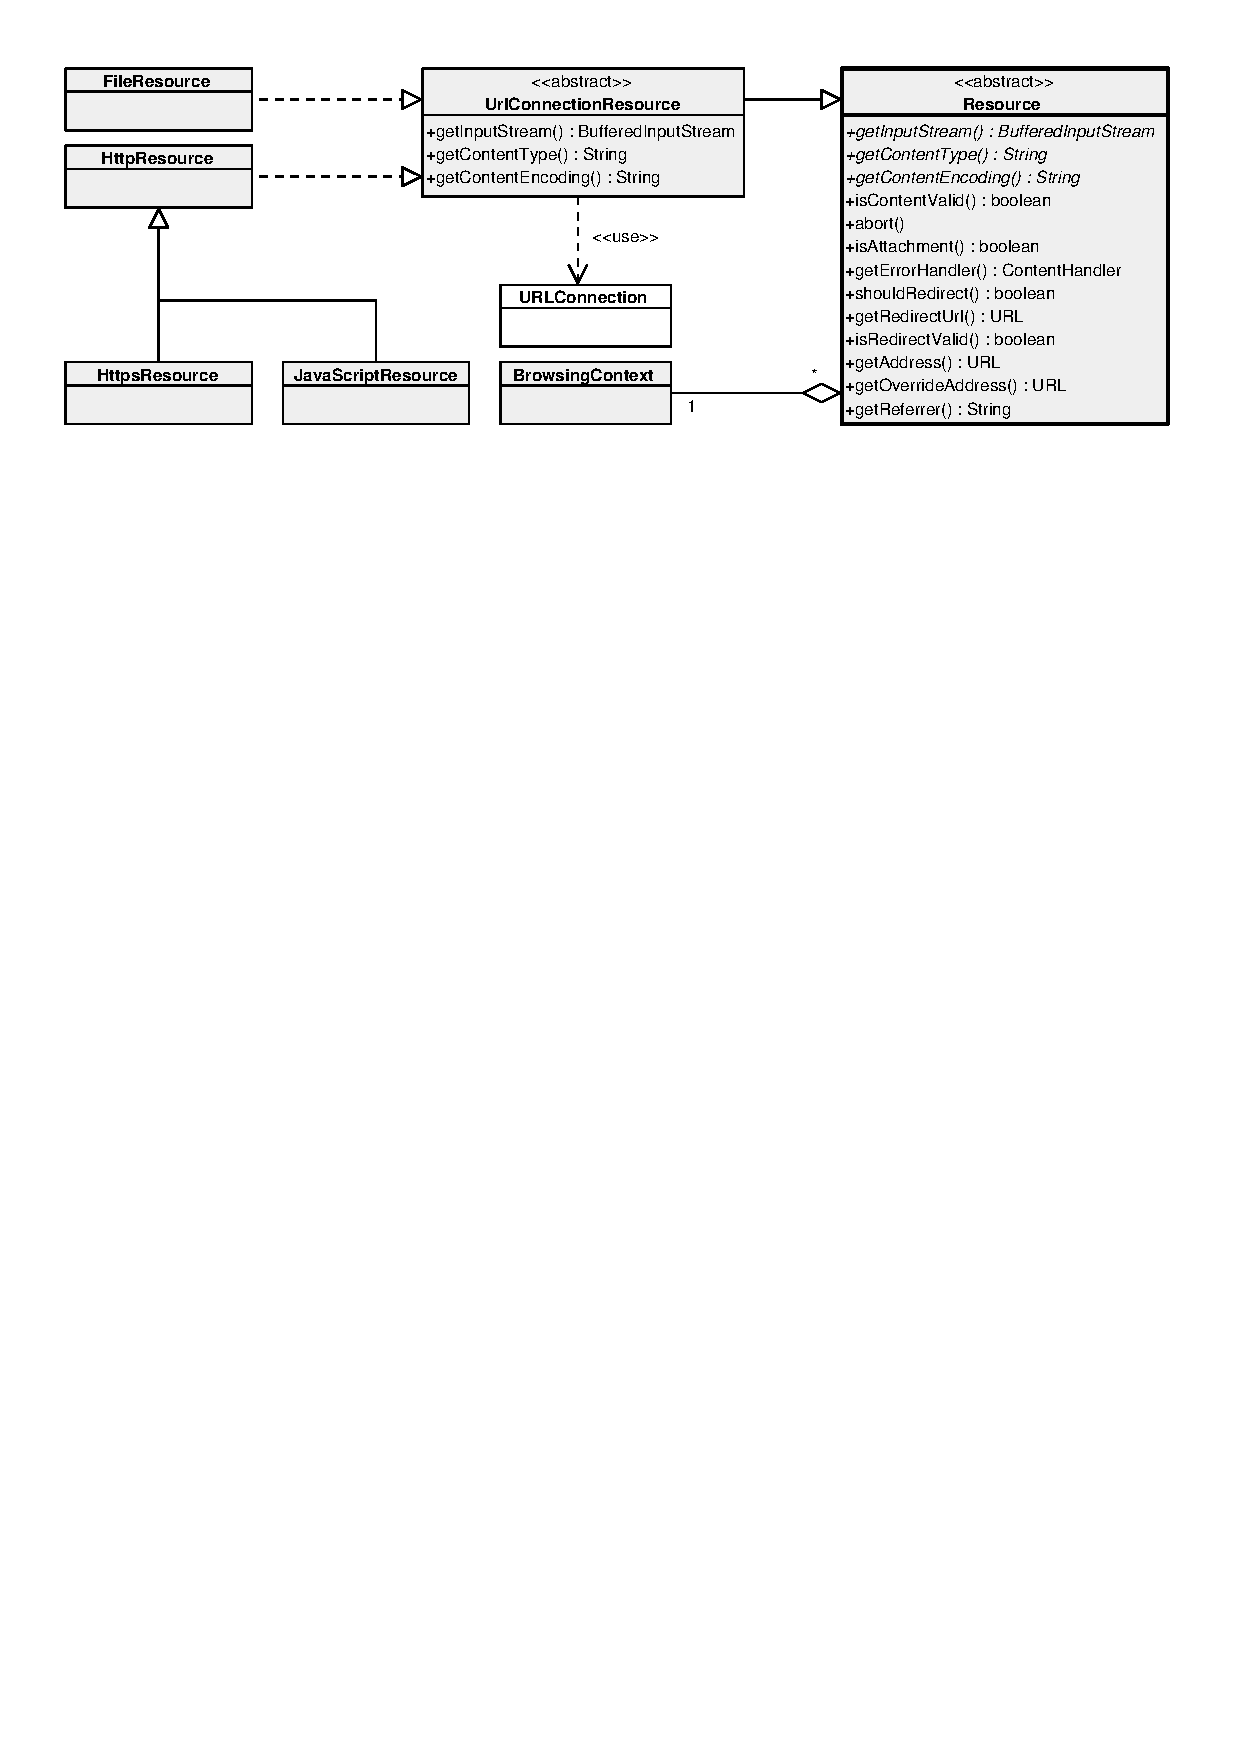
\includegraphics{fig/org-fit-cssbox-scriptbox-resource-Resource.pdf}
    }
    \caption{Diagram tříd znázorňující abstraktní třídu pro všechny zdroje}
    \label{Figure.Resource}
  \end{center}
\end{figure}

Pokud hovoříme o stažení zdroje, máme na mysli navázání připojení a~podle daného protokolu komunikaci se serverem. Komunikaci se serverem a~vytváření konkrétního zdroje zajišťují třídy ovladačů -- třídy rozšiřující abstraktní třídu pro ovladače \texttt{FetchHandler}. Každý konkrétní ovladač vytváří jeden z výše zmíněných specifických zdrojů (obrázek \ref{Figure.FetchRegistry}). Pro stažení zdroje je vyčleněna metoda \texttt{fetch()}, která vnitřně zavolá chráněnou metodu \texttt{fetchImpl()}. Pokud byl ovladač vytvořen v~synchronním módu, pak tato operace způsobí blokování do doby stažení zdroje. Pro získání nově staženého zdroje slouží metoda \texttt{getResource()}, která také volá chráněnou metodu, tentokrát \texttt{getResourceImpl()}. 

\begin{figure}[H]
  \begin{center}
    \scalebox{0.80}{
      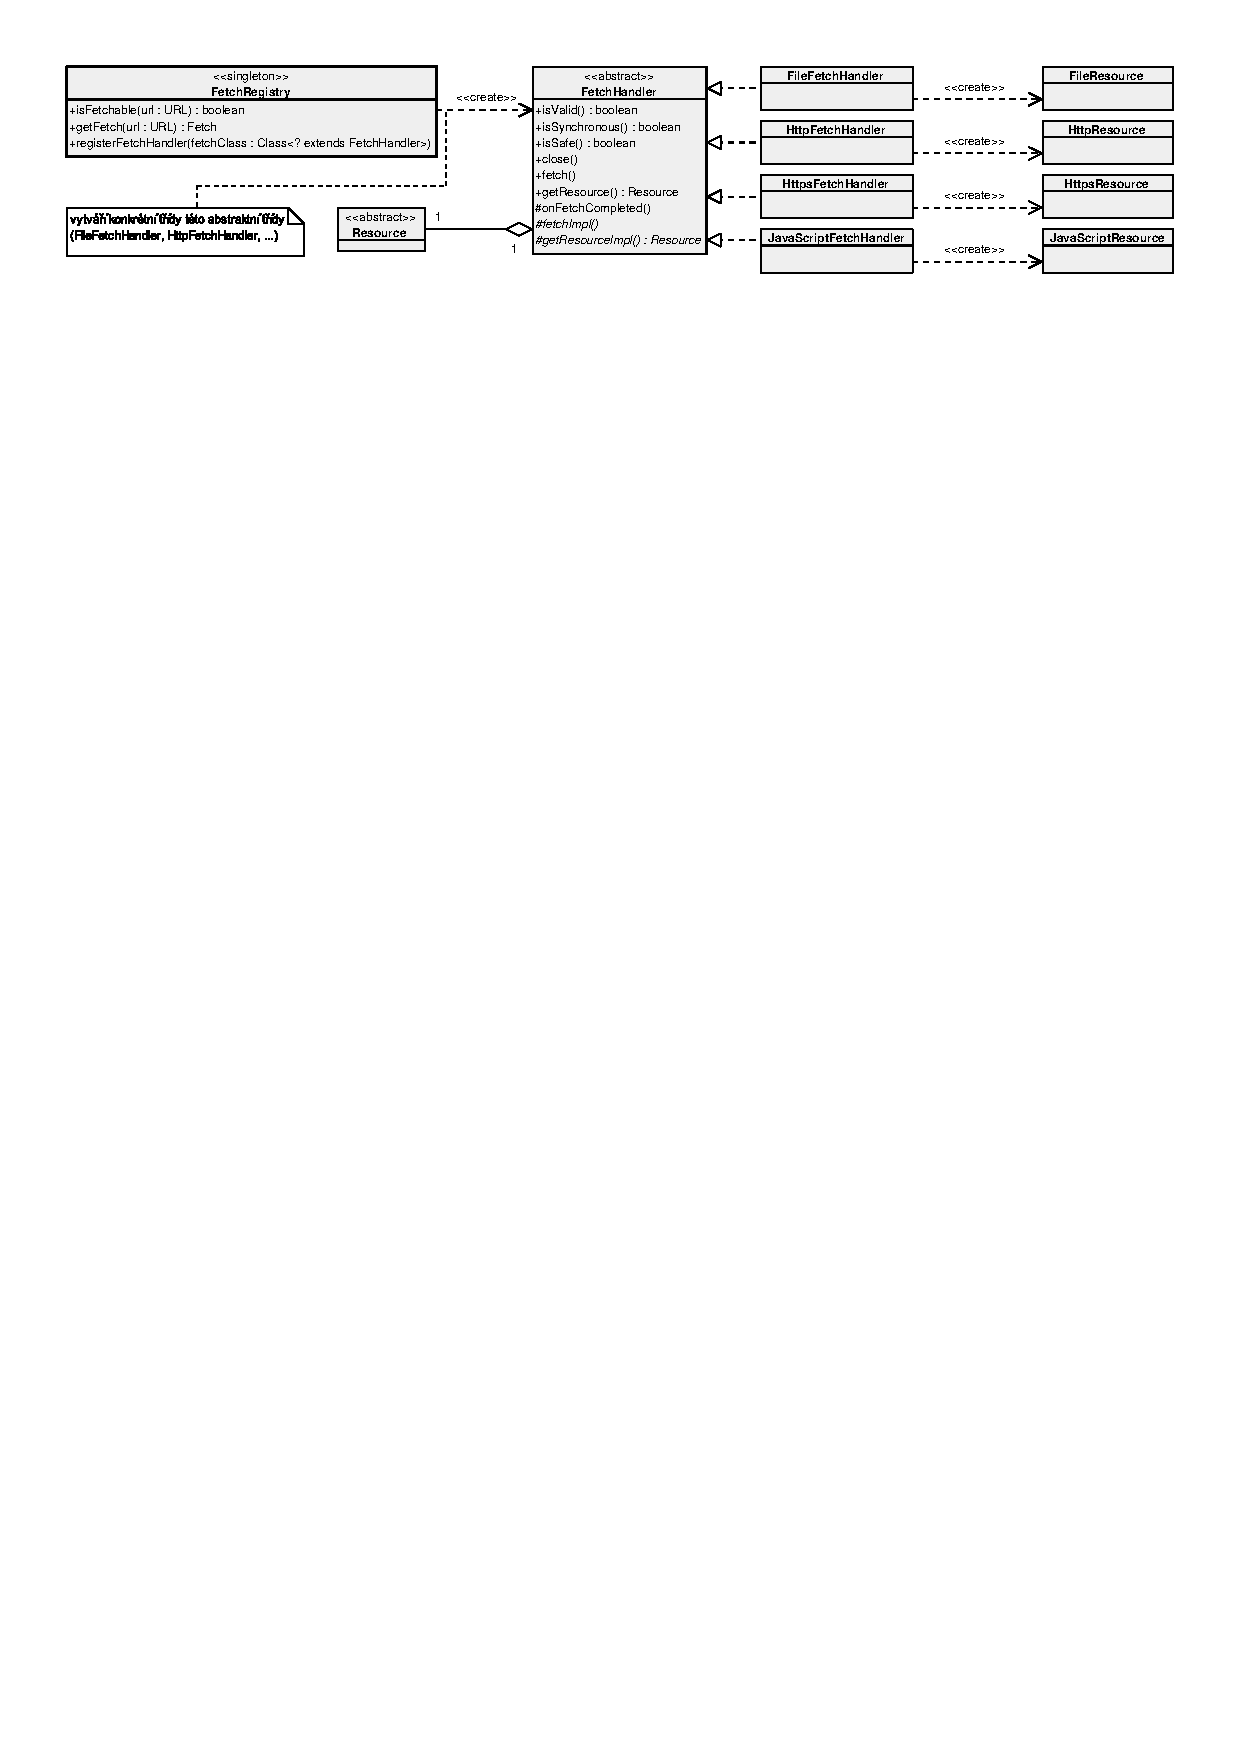
\includegraphics{fig/org-fit-cssbox-scriptbox-resource-FetchRegistry.pdf}
    }
    \caption{Diagram tříd znázorňující registr ovladačů}
    \label{Figure.FetchRegistry}
  \end{center}
\end{figure}

V~praxi při získávání zdroje máme k dispozici pouze jeho URL. Nevíme předem, jaký ovladač pro jeho stažení použít. Přesto bychom chtěli mít jednotné rozhraní, které by převzalo předanou URL a~vyhodnotilo, zda je zdroj stažitelný, popř. ho i stáhlo. Za tímto účelem vznikl registr všech ovladačů \texttt{FetchRegistry}, který shromažďuje všechny podporované ovladače a~umožňuje nad nimi vyhledávat podle protokolu předané URL. Registr registruje třídy ovladačů a~vytváří na ně asociace v~závislosti na tom, jaké protokoly podporují. Podporované protokoly jsou získávány ze speciální anotace třídy \texttt{FetchHandlerPreamble}, která musí být přítomna u každé třídy registrovaného ovladače.

\subsection{Zpracovávání obsahu zdrojů}
\label{Chapter.Implementation.ContentHandling}

V~předešlé kapitole \ref{Chapter.Implementation.DownloadingResources} bylo popsáno, jak lze získávat zdroje. Zdroje musí být ovšem v~závislosti na typu obsahu dále zpracovávány, převedeny na dokument a~až poté mohou být zobrazeny. Pro zpracovávání byla zvolena podobná návrhová myšlenka jako pro získávání zdrojů. Byl implementován registr továren ovladačů \texttt{ContentHandlerRegistry}, který spravuje továrny ovladačů pro různé typy obsahů a~získává instance ovladačů v~závislosti na požadovaném MIME typu obsahu.

\begin{figure}[H]
  \begin{center}
    \scalebox{0.80}{
      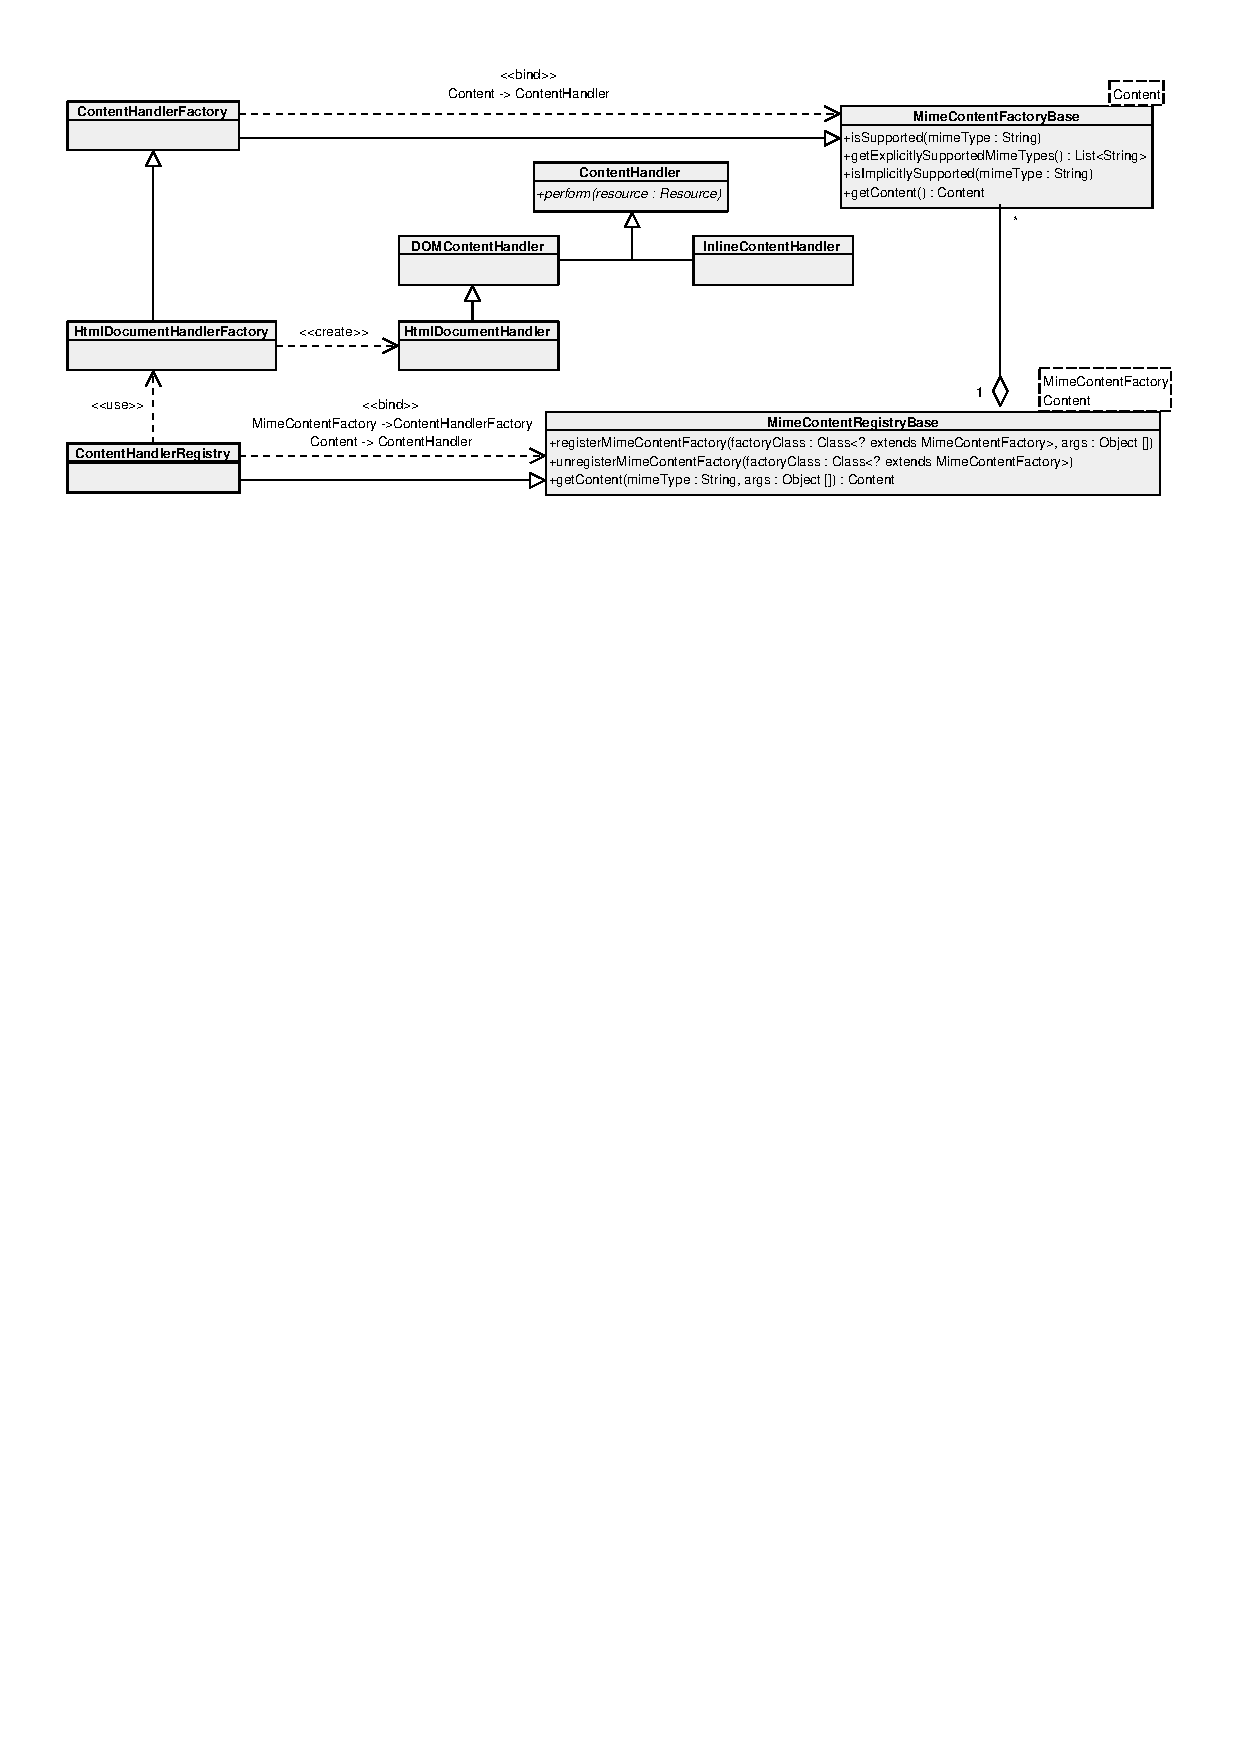
\includegraphics{fig/org-fit-cssbox-scriptbox-resource-ContentHandlerRegistry.pdf}
    }
    \caption{Diagram tříd znázorňující registr továren ovladačů}
    \label{Figure.ContentHandlerRegistry}
  \end{center}
\end{figure}

Třída ovladače, která zajišťuje zpracovávání daného typu obsahu, musí být konkrétní třídou nad abstraktní třídou \texttt{ContentHandler}. Pro zpracování obsahu se volá veřejná metoda \texttt{perform()}, která přijímá zdroj ke zpracování. V~současné době je implementován pouze jeden ovladač -- na zpracovávání HTML dokumentů \texttt{HtmlDocumentHandler}, který vkládá do událostní smyčky úlohu, jež zajišťuje tvorbu dokumentu, přidání nového dokumentu do historie, její aktualizaci a~v~poslední řadě zahájení parsování dokumentu. V~implementaci jsou také připraveny návrhy tříd ovladačů na zpracovávání obrázků, textových souborů, XML dokumentů, médií, aj.

Z důvodu potřeby podobné funkčnosti v~jiné části implementace -- výběru skriptovacího enginu v~závislosti na MIME typu skriptu (viz kapitola \ref{Chapter.Implementation.ScriptEngines}) byly implementovány generické třídy pro správu továren objektů jakéhokoliv~typu. Abstraktní továrna, která obsluhuje získávání obsahů podporovaného MIME typu, je v~implementaci reprezentována třídou \texttt{MimeContentFactoryBase}. Každá konkrétní továrna redefinuje metodu pro vytváření obsahu \texttt{getContent()} a~metody pro zjištění podporovaných MIME typů. Rozlišujeme dva druhy MIME typů:

\begin{itemize}
  \item \textbf{explicitně podporované} -- typy, které předem můžeme určit, a~o kterých víme, že továrna bude tyto typy podporovat, tzn. známe celou jejich podobu, např. \texttt{text/html}. Pro zjištění těchto typů slouží metoda \texttt{getExplicitlySupportedMimeTypes()};
  \item \textbf{implicitně podporované} -- typy, kde rozhodne o jejich platnosti až jejich formát, částečná shoda, např. pouze prefix \texttt{text/}; Pro test, zda se jedná o implicitně podporovaný typ je vyčleněná metoda \texttt{isImplicitlySupported()}.
\end{itemize}

\subsection{Navigace mezi dokumenty}
\label{Chapter.Implementation.DocumentNavigation}

V~kapitole \ref{Chapter.Implementation.DownloadingResources} byla popsána metodika, jak se získávají zdroje, jež lze využít nejenom pro stahování dokumentů, ale i pro získávání souborů kaskádových stylů nebo externích skriptů během načítání stránky. Předchozí kapitola \ref{Chapter.Implementation.ContentHandling} se zabývala výhradně zpracováním obsahu zdroje, vytvářením dokumentu a~jeho zobrazením. Celý proces, který zahrnuje stažení zdroje a~následné zobrazení dokumentu, přičemž je změněn předchozí aktivní dokument, lze nazvat navigací mezi dokumenty.

Požadavky na navigování nového dokumentu mohou přicházet asynchronně. V~implementaci je vstupním bodem pro příchod nových požadavků navigační kontroler -- třída \texttt{NavigationController}. Kontroler všechny požadavky registruje a~pokouší se je obsloužit. Obsluha požadavků je delegována třídě požadavku \texttt{NavigationAttempt}, která o aktuálním stavu zpracování požadavku informuje svůj kontroler pomocí callback metod rozhraní \texttt{NavigationAttemptCallback}. Callback metody informují o následujících stavech:

\begin{itemize}
  \item \textbf{vyzrání} -- navigovaný dokument byl přidán do historie, ale stále není kompletní;
  \item \textbf{zrušení} -- navigace byla zrušena uživatelem nebo kvůli nějaké chybě;
  \item \textbf{dokončení} -- navigace byla kompletně provedena; 
  \item \textbf{výběru kontextu} -- byl vybrán efektivního procházecí kontext pro navigaci.
\end{itemize}

Navigace přechází do jednotlivých stavů zavoláním korespondujících metod navigace: \texttt{complete()}, \texttt{cancel()} nebo \texttt{mature()}. V~závislosti na tom, jaká callback metoda byla navigačním požadavkem zavolána, je v~navigačním kontroleru provedena k tomu odpovídající akce. Při výběru cílového kontextu je požadavek zaregistrován v~kontroleru, naopak při zrušení nebo dokončení požadavku je požadavek zcela odregistrován. Jelikož bylo žádoucí informovat o stavech provádění požadavků uvnitř navigačního kontroleru i vnější okolí, byl vytvořen opět jednoduchý observer nad navigačním kontrolerem. Události, které mohou být vyvolány, kopírují metody callback volání z navigačního požadavku. 

\begin{figure}[H]
  \begin{center}
    \scalebox{0.75}{
      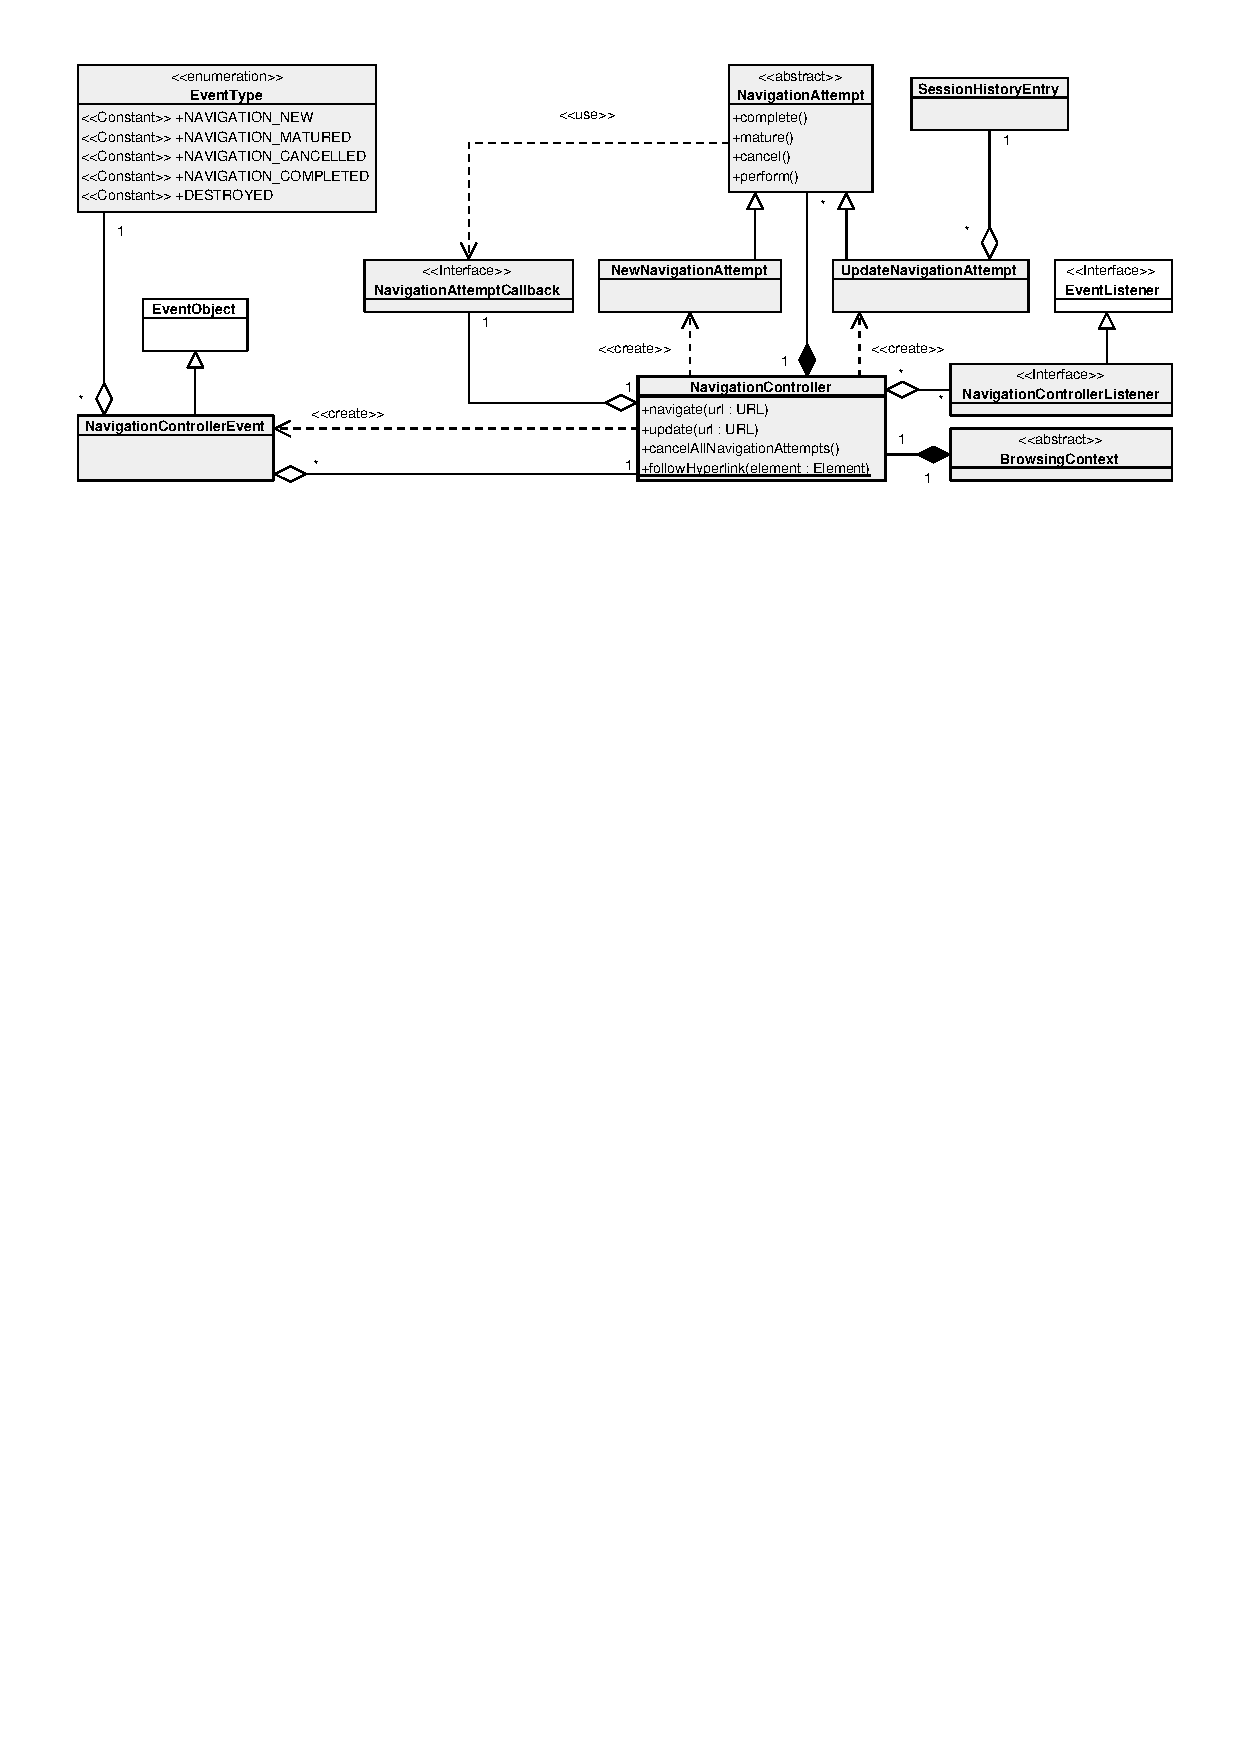
\includegraphics{fig/org-fit-cssbox-scriptbox-navigation-NavigationController.pdf}
    }
    \caption{Diagram tříd znázorňující navigační kontroler}
    \label{Figure.NavigationController}
  \end{center}
\end{figure}

\vspace{-1em}

Navigační kontroler vytváří celkem dva typy navigací. Prvním typem navigace je navigace \texttt{NewNavigationAttempt}, která vzniká po zavolání metody \texttt{navigate()} a~která přidává do historie nový navigovaný dokument. Druhý typ navigace \texttt{UpdateNavigationAttempt} vznikající zavoláním metody \texttt{update()} přepíše dokument předaného záznamu historie, který je tímto aktualizován.

\bigskip \noindent K vytvoření navigačního požadavku je zapotřebí nastavit:  

\begin{itemize}
  \item \textbf{\texttt{navigationController}} -- navigační kontroler, který vlastní tento požadavek;
  \item \textbf{\texttt{sourceBrowsingContext}} -- cílový procházecí kontext, kde navigovace probíhat;
  \item \textbf{\texttt{url}} -- adresu navigovaného zdroje;
  \item \textbf{\texttt{exceptionEnabled}} -- nastaveno pokud se mají generovat DOM výjimky;
  \item \textbf{\texttt{explicitSelfNavigationOverride}} -- když je nastaveno, bude cílovým procházecím kontextem zvolen procházecí kontext navigačního kontroleru a~nebude se vyhodnocovat efektivní procházecí kontext;
  \item \textbf{\texttt{replacementEnabled}} -- nastaveno pokud žádáme, aby byl přepsán právě aktivní záznam historie a~smazány všechny jeho následující záznamy.
\end{itemize}

Pro vykonání a~spuštění navigačního algoritmu je vyčleněná metoda \texttt{perform()}. Algoritmus provádí zjednodušeně následující body:

\begin{itemize}
  \item \textbf{bezpečnostní kontroly} -- testuje se, zda lze navigovat cílový procházecí kontext;
  \item \textbf{výběr efektivního cílového procházecího kontextu} -- pokud není navigace prováděna v~procházecím kontextu \texttt{<iframe>} se seamless atributem elementu, pak je efektivní cílový kontext vždy totožný s vybraným cílovým procházecícm kontextem;
  \item \textbf{navigace na fragment dokumentu} -- když navigujeme pouze fragment dokumentu, pak se provede okamžitá navigace na pozici fragmentu, aktualizuje se historie a~tímto bodem navigace ihned končí; 
  \item \textbf{uvolnění dokumentu} -- aktivní dokument cílového kontextu je uvolněn;
  \item \textbf{získání ovladače na stažení zdroje} -- při úspěchu přechází navigační požadavek do asynchronního zpracovávání;
  \item \textbf{přesměrování} -- když je zapotřebí přesměrovat na jiný zdroj;
  \item \textbf{získání ovladače} -- vyhledání ovladače v~registru \texttt{ContentHandlerRegistry}; 
  \item \textbf{zpracování zdroje} -- zavolání metody \texttt{perform()} nad vyhledaným ovladačem.
\end{itemize}

Výše popsané třídy navigování se týkaly jádra uživatelského agenta. Navigovat dokumenty je ovšem přístupné i z klientského JavaScriptu. Pro tento účel slouží veřejné rozhraní \texttt{Location}, které bylo také zcela implementováno (obrázek \ref{Figure.Location}). Každý dokument procházecího kontextu vlastní unikátní instanci tohoto rozhraní.

\begin{figure}[H]
  \begin{center}
    \scalebox{0.55}{
      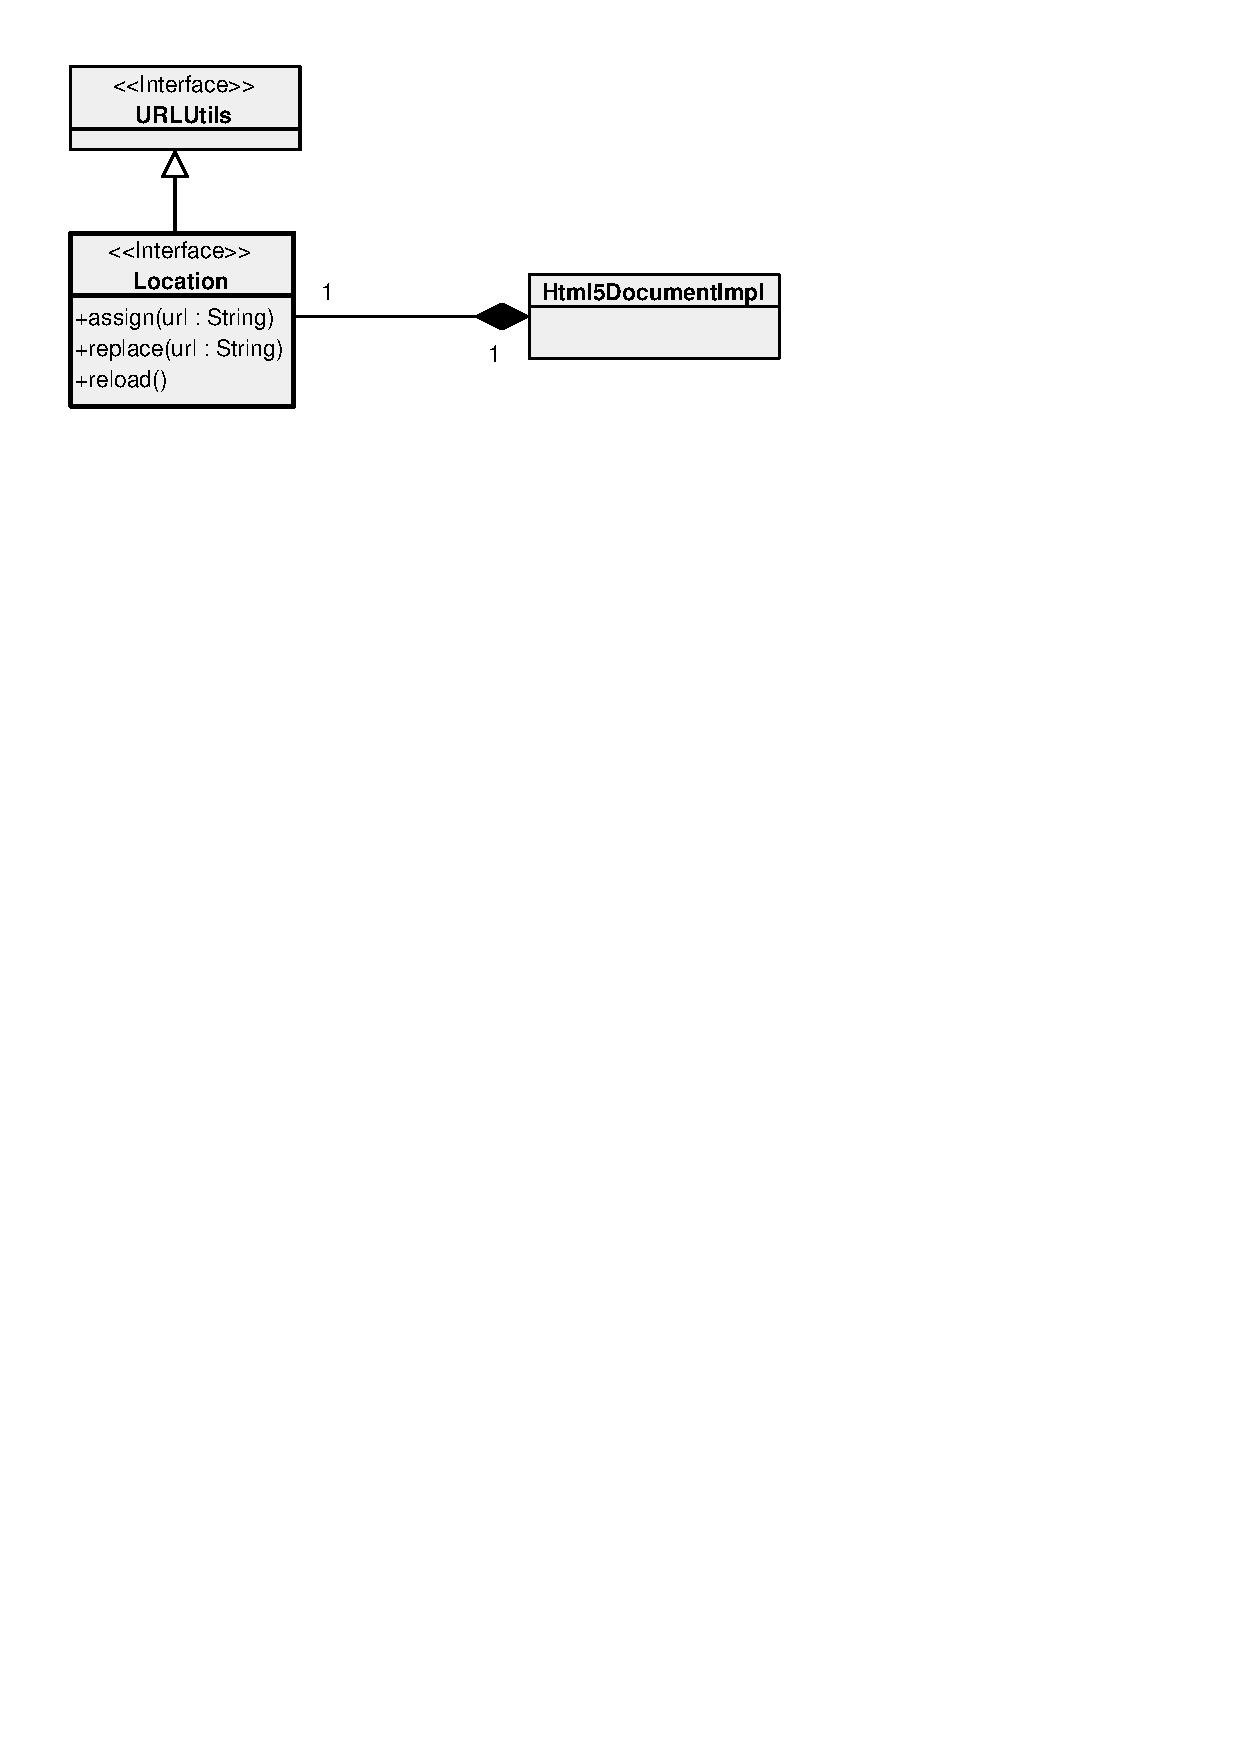
\includegraphics{fig/org-fit-cssbox-scriptbox-navigation-Location.pdf}
    }
    \caption{Diagram tříd znázorňující rozhraní Location}
    \label{Figure.Location}
  \end{center}
\end{figure}
 
Pro implementaci bylo využito navigačního kontroleru. Metody \texttt{assign()} a~\texttt{reload()} volají metodu kontroleru \texttt{navigate()} s nastaveným příznakem \texttt{replacementEnabled}. Metoda \texttt{assign()} naviguje nový dokument bez přepsání právě aktivního dokumentu, příznak \texttt{replacementEnabled} není nastaven. Všechny metody nastavují \texttt{exceptionEnabled}, takže jsou navigačním požadavkem generovány bezpečnostní výjimky.

\subsection{Procházení historie}
\label{Chapter.Implementation.TraversingHistory}

Během navigování stránek dochází ke změně aktivních dokumentů. Všechny předchozí navigované dokumenty jsou nadále uchovávány v~historii sezení. Průchodem historie sezení jde kdykoliv~navracet dokumenty, které nejsou momentálně aktivní v~současném procházecím kontextu. Historie sezení se vytváří v~rámci konstrukce procházecího kontextu, jenž danou historii vlastní. Historii sezení si lze představit jako pole všech někdy navigovaných dokumentů s ukazatelem na aktivní dokument procházecího kontextu (obrázek \ref{Figure.SessionHistory}).

\begin{figure}[H]
  \begin{center}
    \scalebox{0.50}{
      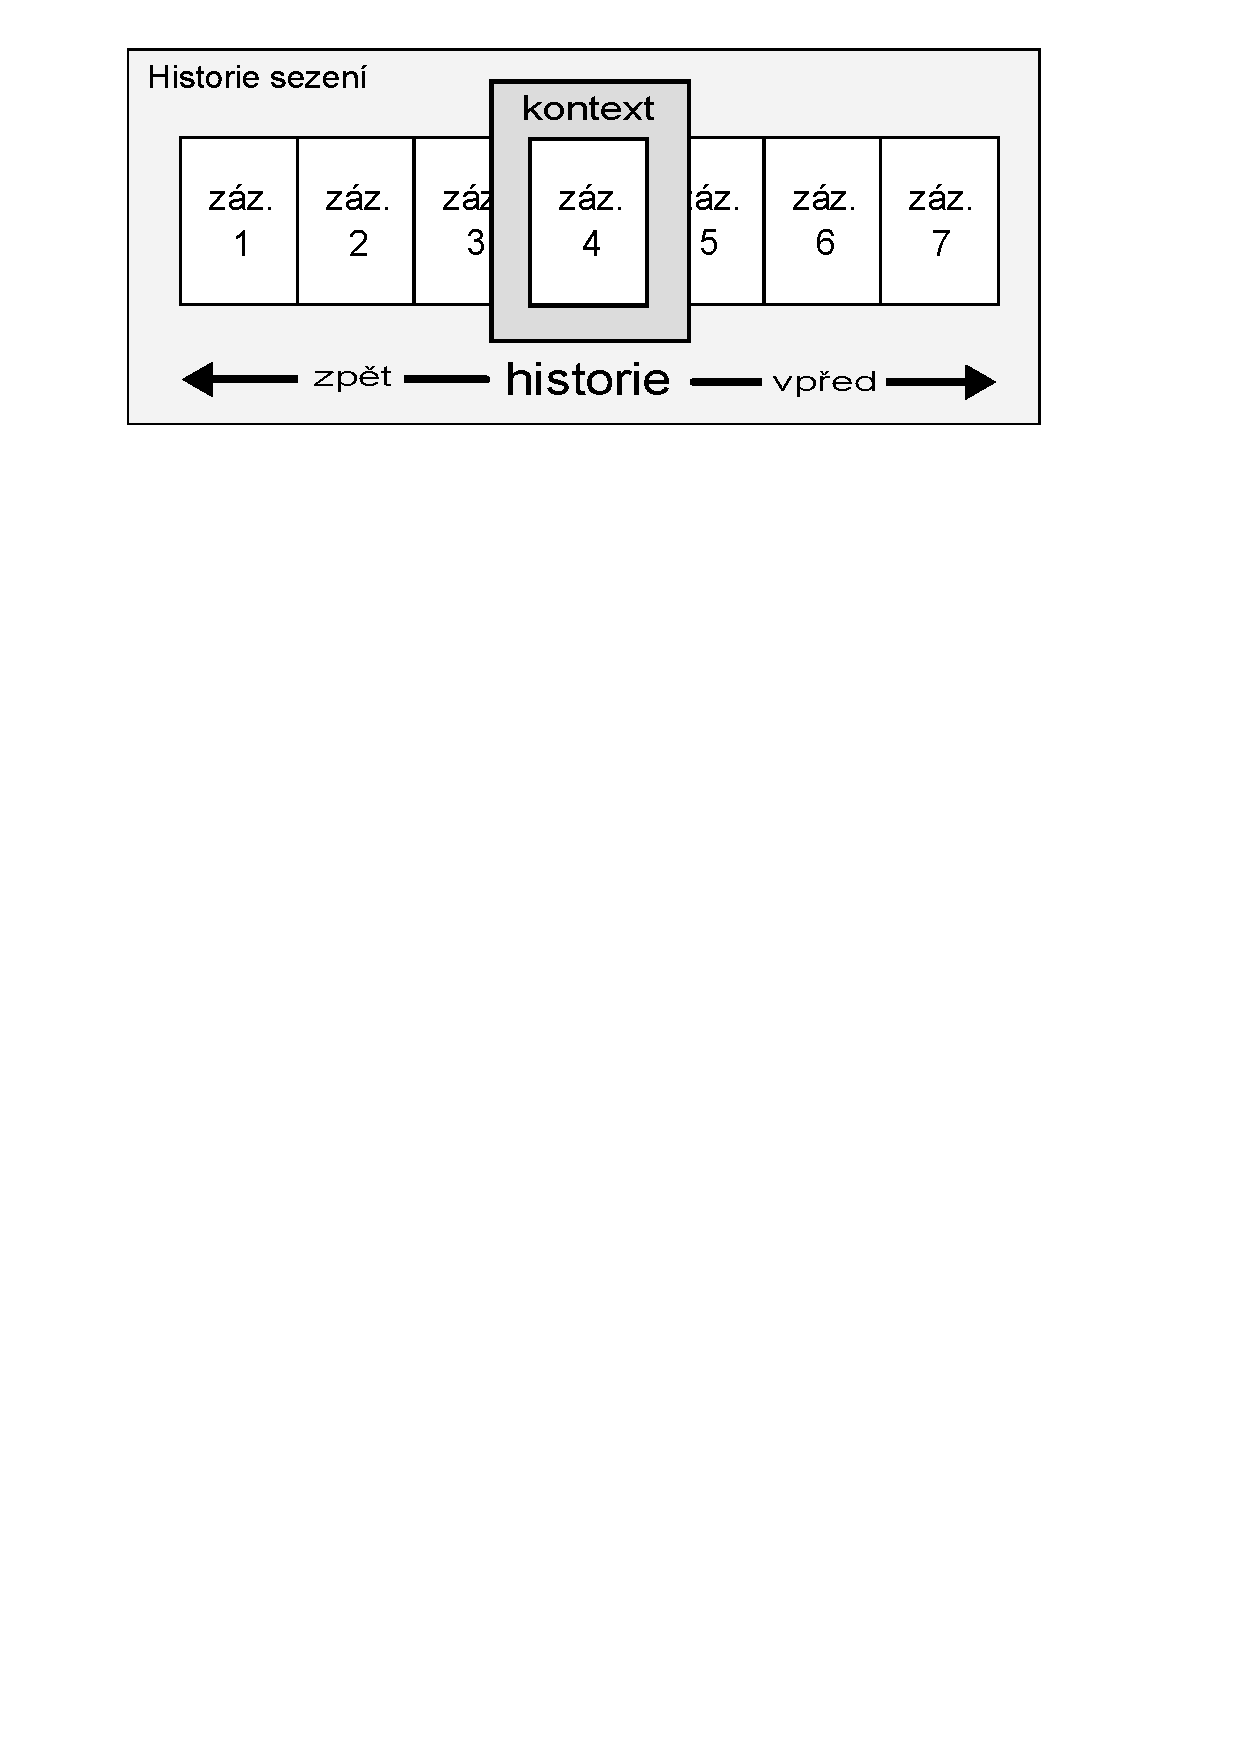
\includegraphics{fig/history.pdf}
    }
    \caption{Vizualizace historie sezení se záznamy mezi kterými lze posouvat}
    \label{Figure.SessionHistory}
  \end{center}
\end{figure}

\vspace{-1em}

V~implementaci je historie sezení představována třídou \texttt{SessionHistory} (obrázek \ref{Figure.SessionHistoryDiagram}). Je implementována jako lineární list záznamů historie \texttt{SessionHistoryEntry}. Záznam historie musí minimálně uchovávat adresu zdroje, odkud byl dokument získán. Dále by měl záznam obsahovat dokument, který byl vytvořen během navigace, která vytvořila tento záznam. A dodatečně může záznam uchovávat titulek a~datum navštívení stránky, stavový objekt \texttt{StateObject} a~uživatelský kontext \texttt{UserPersistedState}. Stavovým objektem rozumíme objekty, které lze v~historii uchovávat přes rozhraní History, popsané níže. Uživatelským kontextem rozumíme prostor pro ukládání např. pozic posuvníků před přesunutím na jiný záznam historie a~jiné nastavení specifické pro danou HTML stránku. 

\begin{figure}[H]
  \begin{center}
    \scalebox{0.77}{
      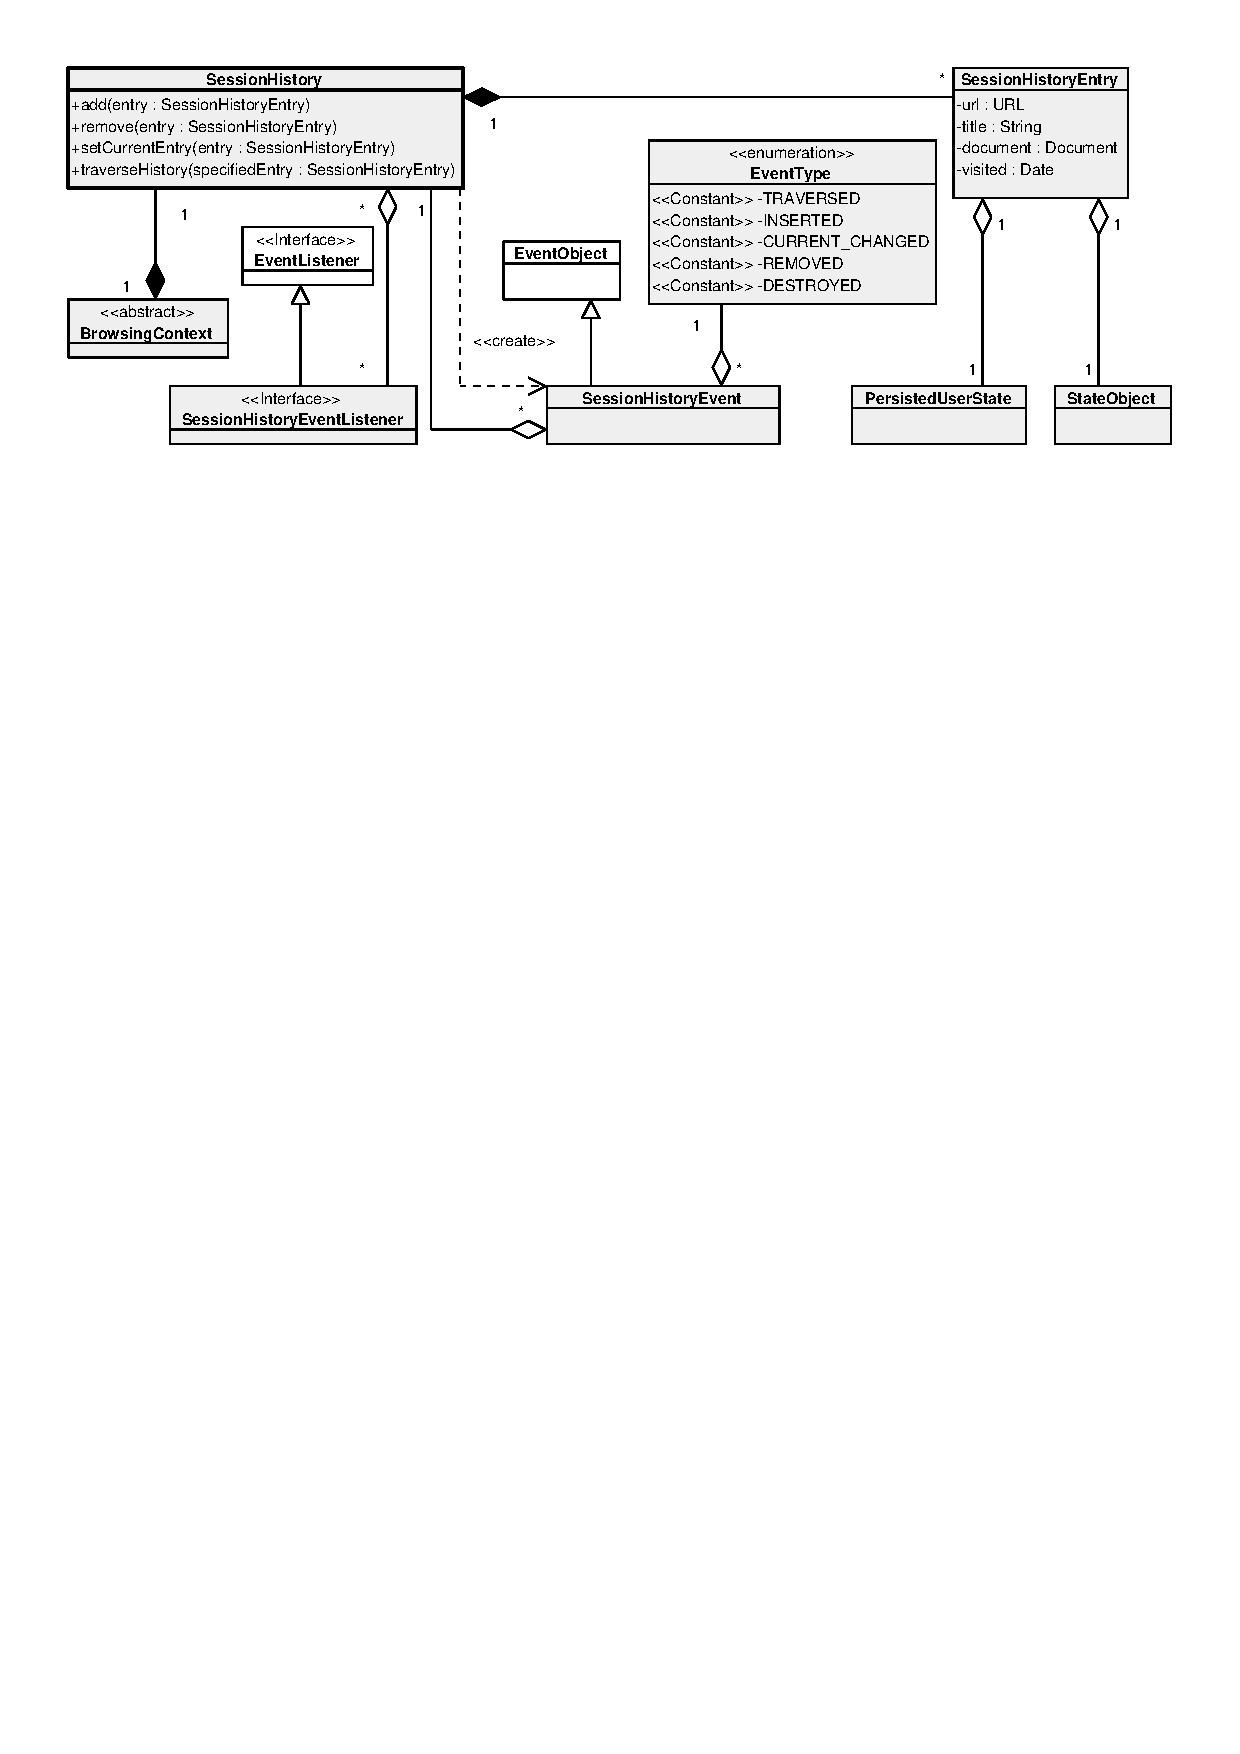
\includegraphics{fig/org-fit-cssbox-scriptbox-history-SessionHistory.pdf}
    }
    \caption{Diagram tříd znázorňující historii sezení}
    \label{Figure.SessionHistoryDiagram}
  \end{center}
\end{figure}

Tak jako u procházecích kontextů a~navigačního kontroleru, implementuje objekt historie sezení jednoduchý observer mechanismus. Typy událostí generované historií sezení jsou:

\begin{itemize}
  \item \textbf{\texttt{TRAVERSED}} -- událost generovaná po dokončení přechodu z jednoho záznamu historie na nový záznam historie;
  \item \textbf{\texttt{INSERTED}} -- vložení nového záznamu na konec listu historie sezení;
  \item \textbf{\texttt{CURRENT\_CHANGED}} -- pokud byl nastaven nový aktuální záznam historie. Událost zároveň značí, že došlo ke změně aktivního dokumentu procházecího kontextu, který vlastní dané historie sezení; 
  \item \textbf{\texttt{REMOVED}} -- smazání záznamu z historie sezení;
  \item \textbf{\texttt{DESTROYED}} -- zrušení historie sezení.
\end{itemize}

Třída sezení historie \texttt{SessionHistory} obsahuje metody pro přidávání záznamů historie, jejich odebírání, filtrování a~nastavování aktivního záznamu. Celý proces průchodu historií a~změny aktivního záznamu na jiný záznam historie je obsáhlejší proces, který zahrnuje více kroků. Průchod historií sezení je implementován metodou \texttt{traverseHistory()}, která bere jako parametr záznam sezení historie, který by měl být zvolen jako aktivní. Během průchodu historií se zjednodušeně provádí následující kroky:

\begin{enumerate}
  \item Zjištění, zda navigovaný záznam obsahuje objekt dokumentu. Pokud není dokument obsažen a~my si přejeme posunout na tuto pozici v~historii, musí se dokument obnovit zavoláním metody \texttt{update()} daného navigačního kontroleru.
  \item Aktualizace uživatelského kontextu -- uchování např. pozic posuvníků.
  \item Odstranění všech úloh, které by byly po průchodu historií neplatné.
  \item Nastavení nového aktivního záznamu historie sezení.
  \item Generování události load, pokud je dokument kompletní.
  \item Smazání všech záznamů před aktivním záznamem, pokud je to požadováno.
  \item Aktualizace uživatelského prostředí z uchovaného uživatelského kontextu.
  \item Kontrola, zda se změnil v~URL fragment nebo stavový objekt a~generování patřičných událostí hashchange nebo popstate.
\end{enumerate}

Pro zpřístupnění procházení historie z kódu klientského JavaScriptu bylo nutné implementovat rozhraní \texttt{History} (\ref{Figure.History}). 

\bigskip

\begin{figure}[H]
  \begin{center}
    \scalebox{0.80}{
      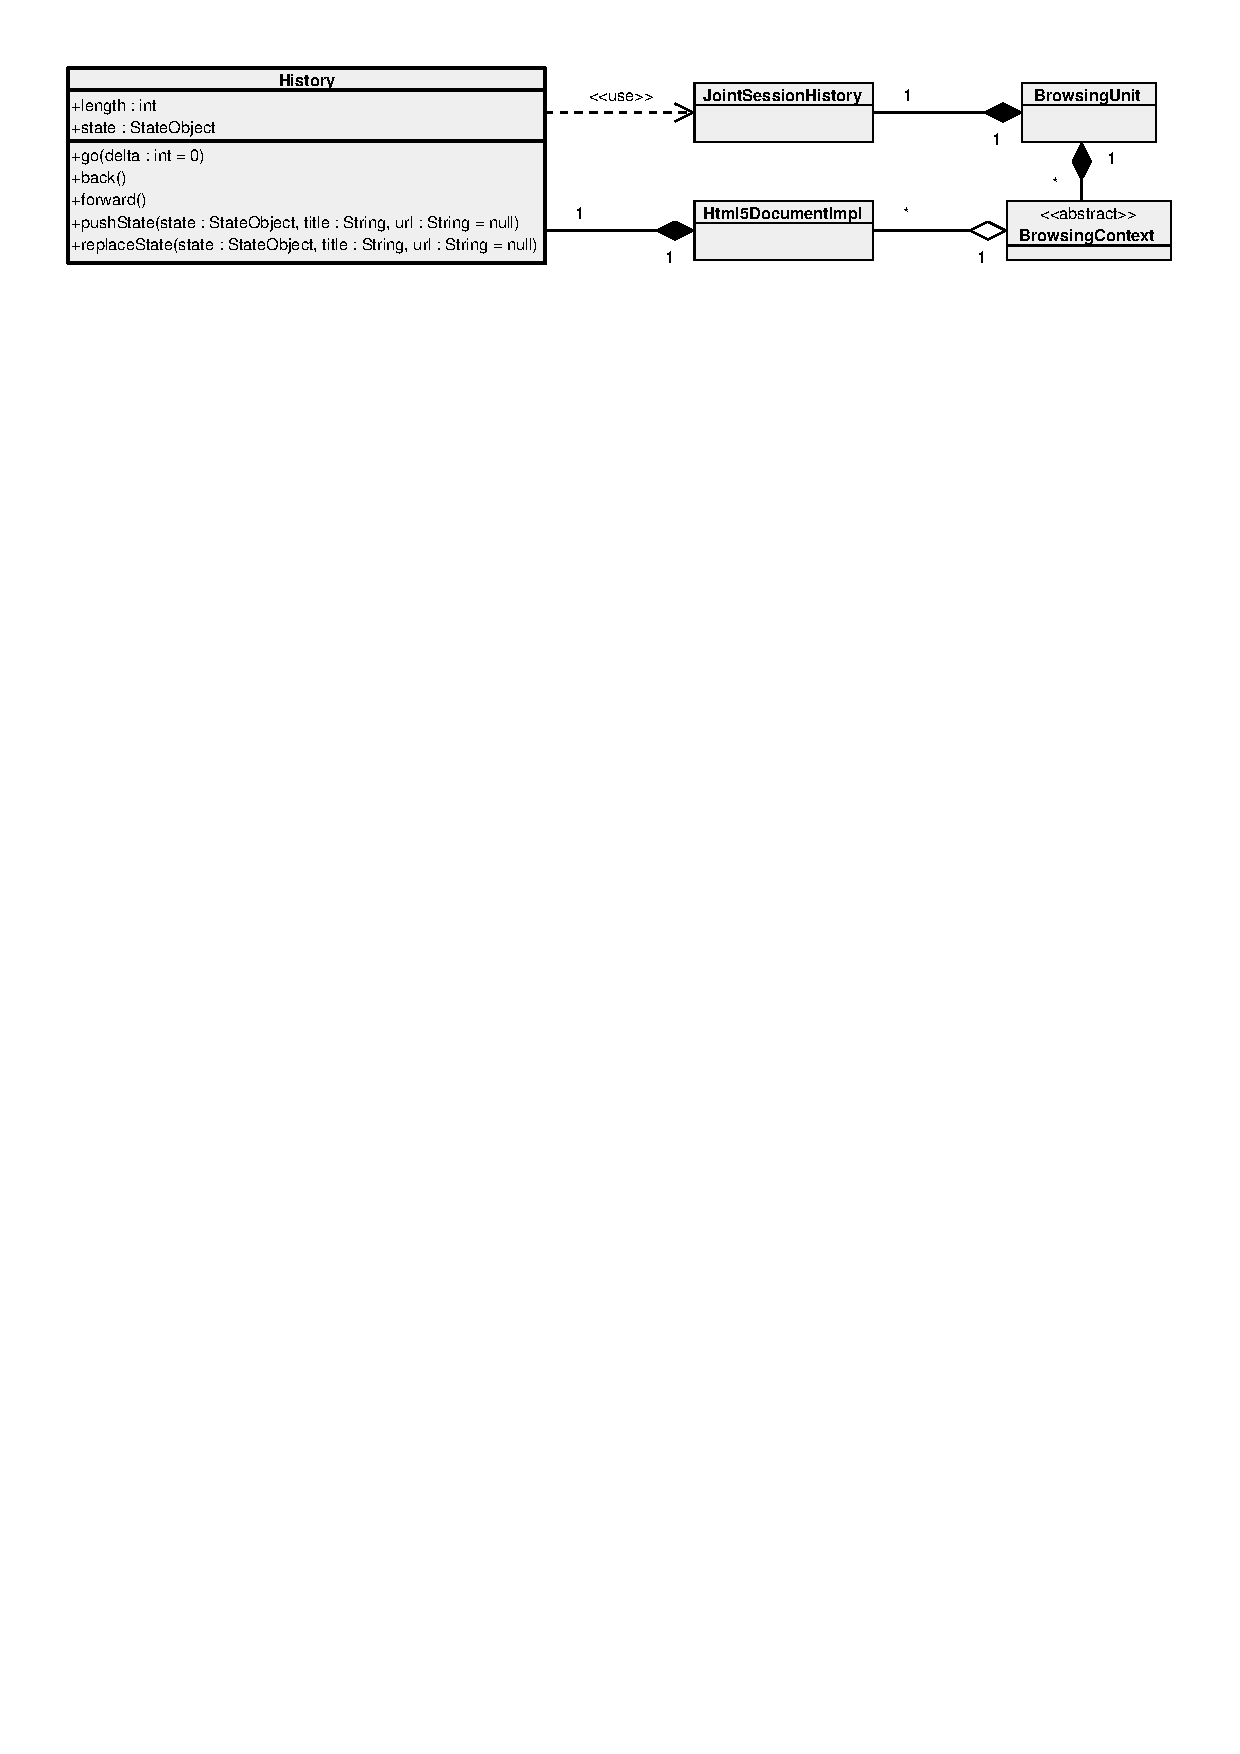
\includegraphics{fig/org-fit-cssbox-scriptbox-history-History.pdf}
    }
    \caption{Diagram tříd znázorňující rozhraní \texttt{History}}
    \label{Figure.History}
  \end{center}
\end{figure}

K implementaci rozhraní \texttt{History} bylo zapotřebí sjednotit všechny historie sezení všech procházecích kontextů procházecí jednotky. Rozhraní \texttt{History} totiž poskytuje procházení všech dokumentů, které kdy byly navigovány v~procházecí jednotce. Spojení všech záznamů historií sezení dané procházecí jednotky proběhlo na základě času jednotlivých záznamů, kdy byly tyto záznamy vytvořeny, neboli kdy byly dokumenty záznamů navigovány. Aktuální záznam společné historie je vždy určen podle posledně vybraného záznamu během průchodu historií sezení v~některém procházecím kontextu procházecí jednotky. Tvorba společné historie sezení je znázorněna na obrázku \ref{Figure.JointSessionHistory}. Čísla záznamu reprezentují unikátní čísla generovaná v~čase, kdy byl záznam vytvořen. Posledně vybraný záznam je záznam hlavního procházecího kontextu s~číslem 4.

\bigskip

\begin{figure}[H]
  \begin{center}
    \scalebox{0.40}{
      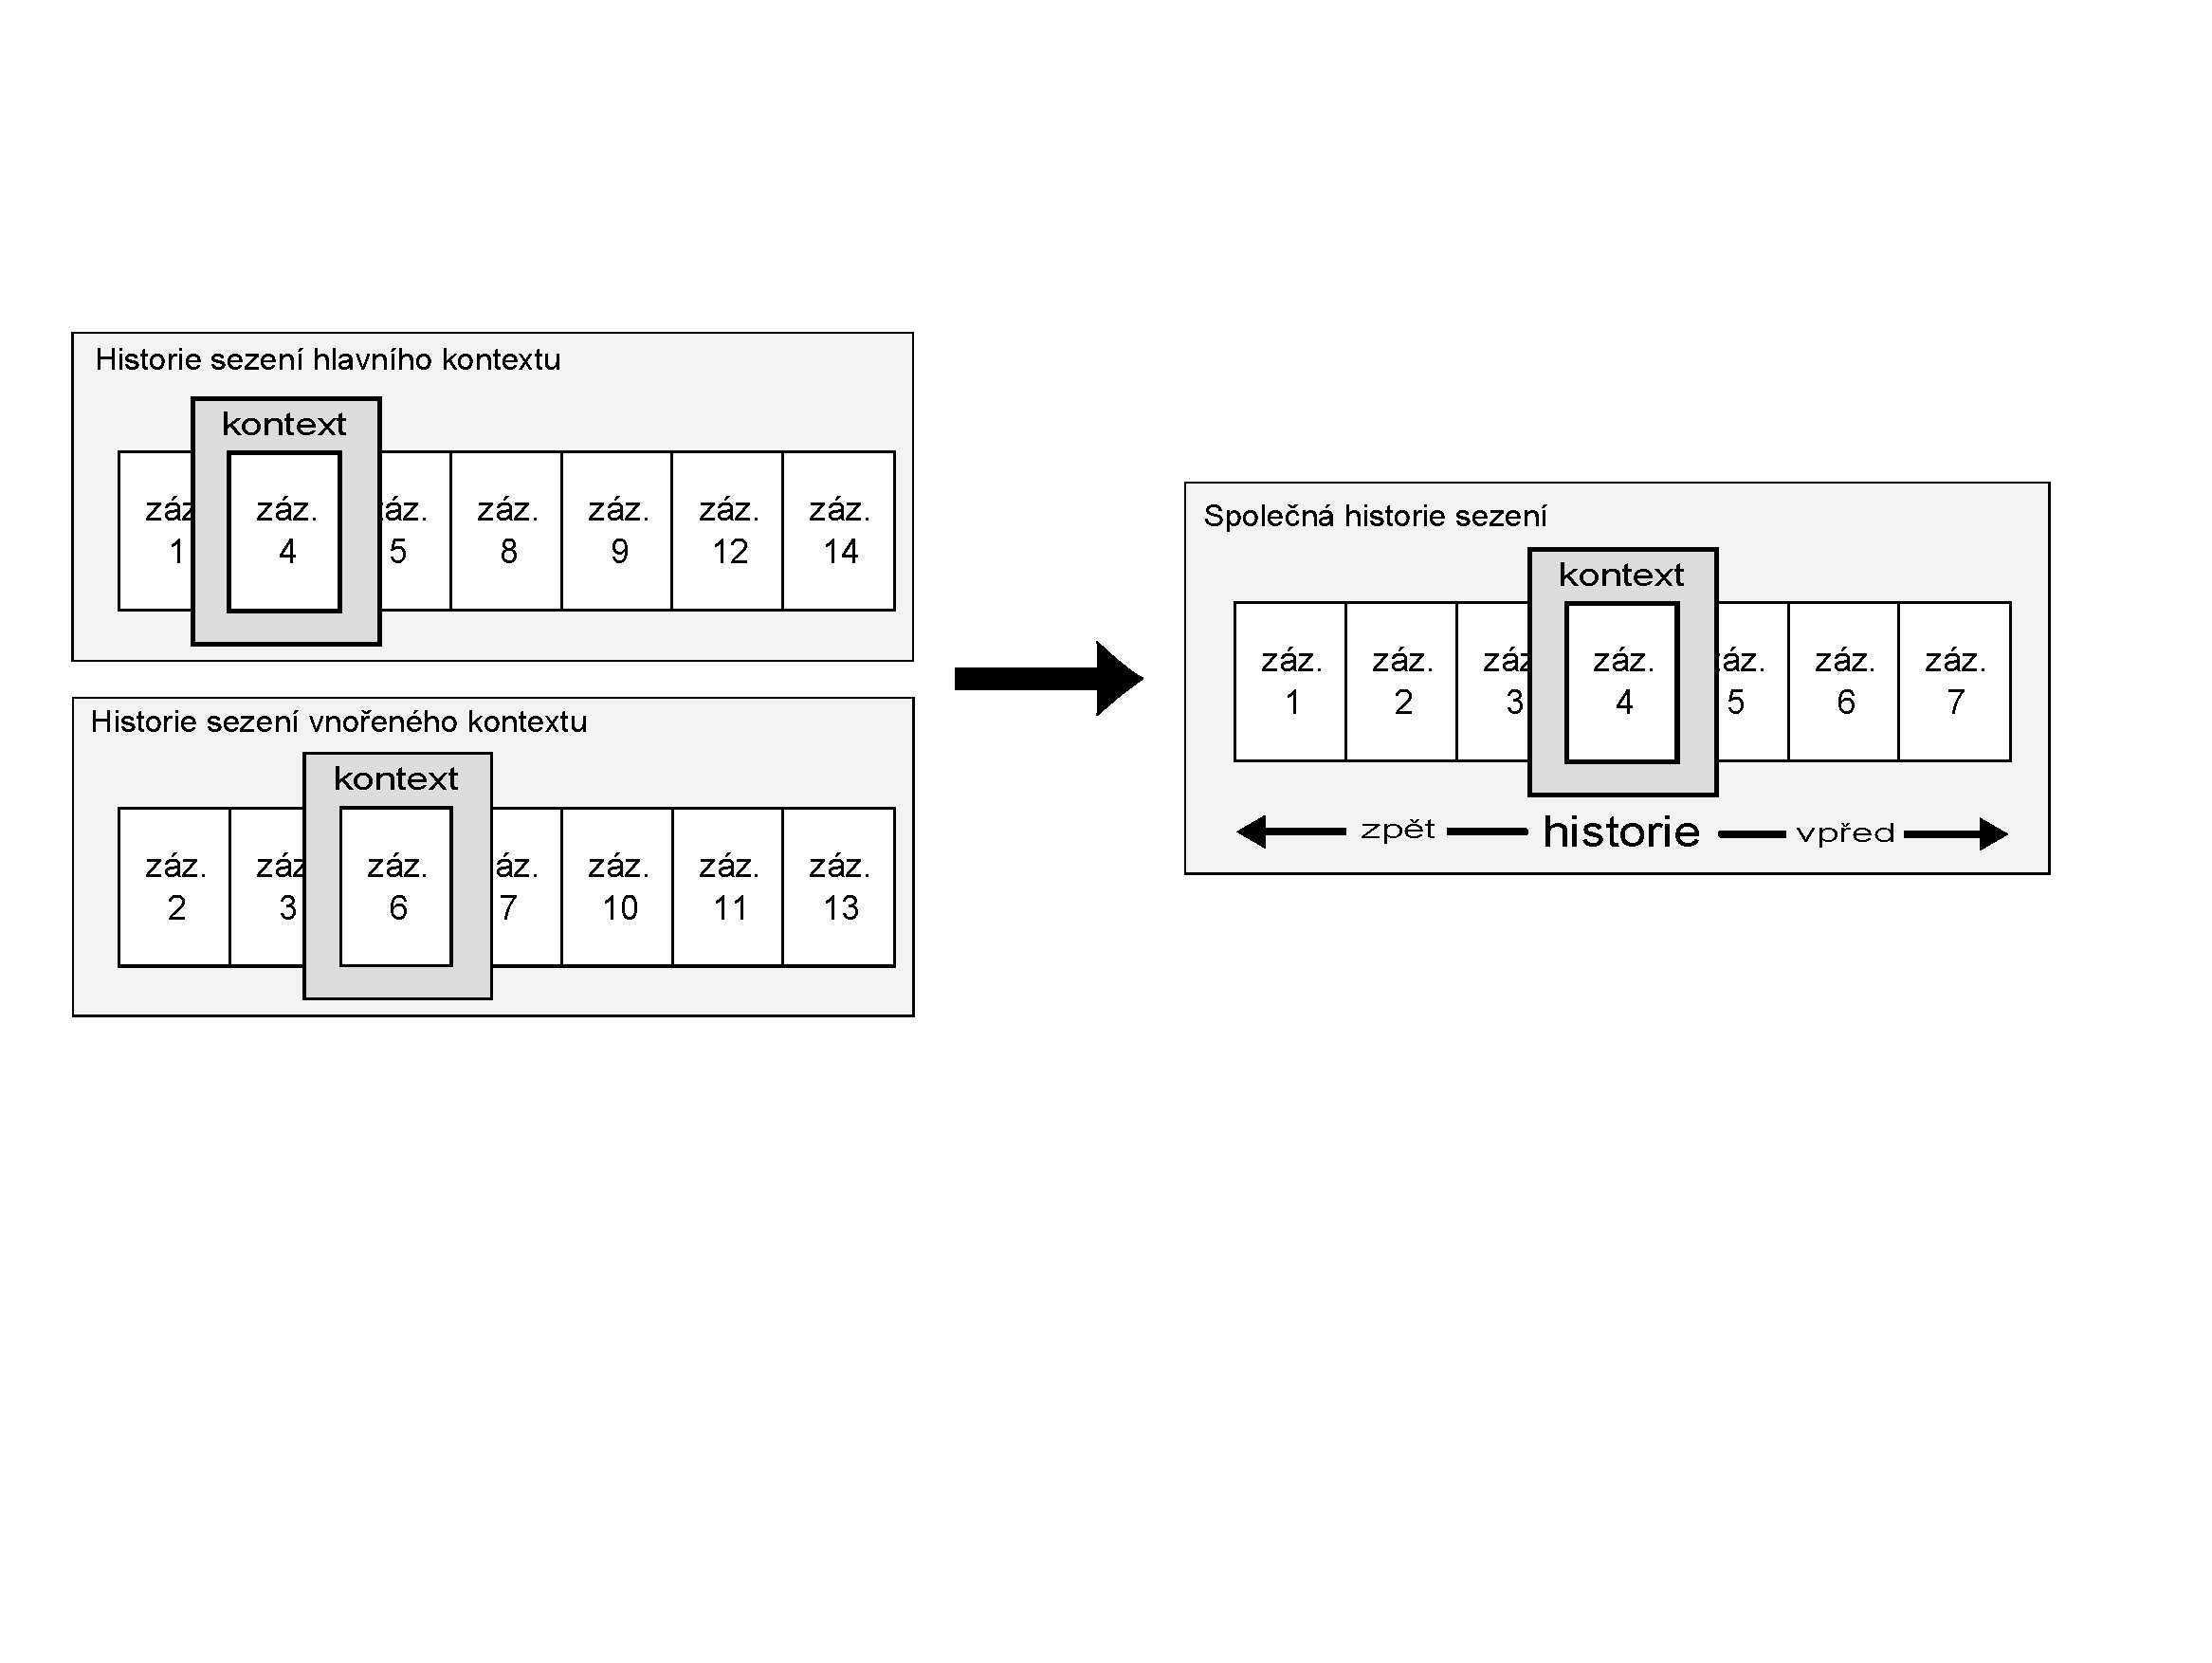
\includegraphics{fig/joint-history.pdf}
    }
    \caption{Vizualizace vytvoření sjednocené historie sezení}
    \label{Figure.JointSessionHistory}
  \end{center}
\end{figure}

Sjednocenou historii sezení vlastní procházecí jednotka. V~implementaci je představována třídou \texttt{JointSessionHistory}. Třída vnitřně registruje \texttt{BrowsingContextListener} a~\texttt{SessionHistoryListener} nad všemi procházecími kontexty a~historiemi sezení procházecí jednotky. Nasloucháním odpovídajících událostí získává neustálé informace o změnách historie, čímž se může sama sebe aktualizovat -- vytvářet sjednocenou historii. Reference na implementaci rozhraní \texttt{History}, jež zpřístupňuje sjednocenou historii z kódu JavaScriptu, se nachází v~dokumentu. Kromě procházení společné historie sezení, rozhraní \texttt{History} umožňuje uchovávat stavový objekt state. Nový stavový objekt můžeme uložit pomocí speciální metody \texttt{pushState()}, která daný objekt nastavuje v~aktuálním záznamu historie sezení. Když procházíme historií, je tento stavový objekt vždy z vybraného záznamu historie přečten a~nastaven do atributu state rozhraní \texttt{History}.

\newpage

\subsection{Dokument a~jeho parsování}
\label{Chapter.Implementation.DocumentParsing}

Ačkoliv~implementace rozhraní dokumentu viditelného z klientského JavaScriptu nebyla cílem této práce, bylo zapotřebí implementovat jeho vnitřní reprezentaci v~kontextu jádra uživatelského agenta. V~dokumentu jsou totiž uchovávány reference na implementovaná rozhraní \texttt{Window}, \texttt{Location} a~\texttt{History}. Zároveň bylo nutno v~dokumentu definovat vytváření elementů \texttt{<iframe>} a~\texttt{<script>} tak, aby jejich implementace odpovídala specifikaci HTML 5. Třída, která reprezentuje implementaci dokumentu je nazvána \texttt{Html5DocumentImpl} a~znázorněna na obrázku \ref{Figure.DocumentImpl}. 

\begin{figure}[H]
  \begin{center}
    \scalebox{0.75}{
      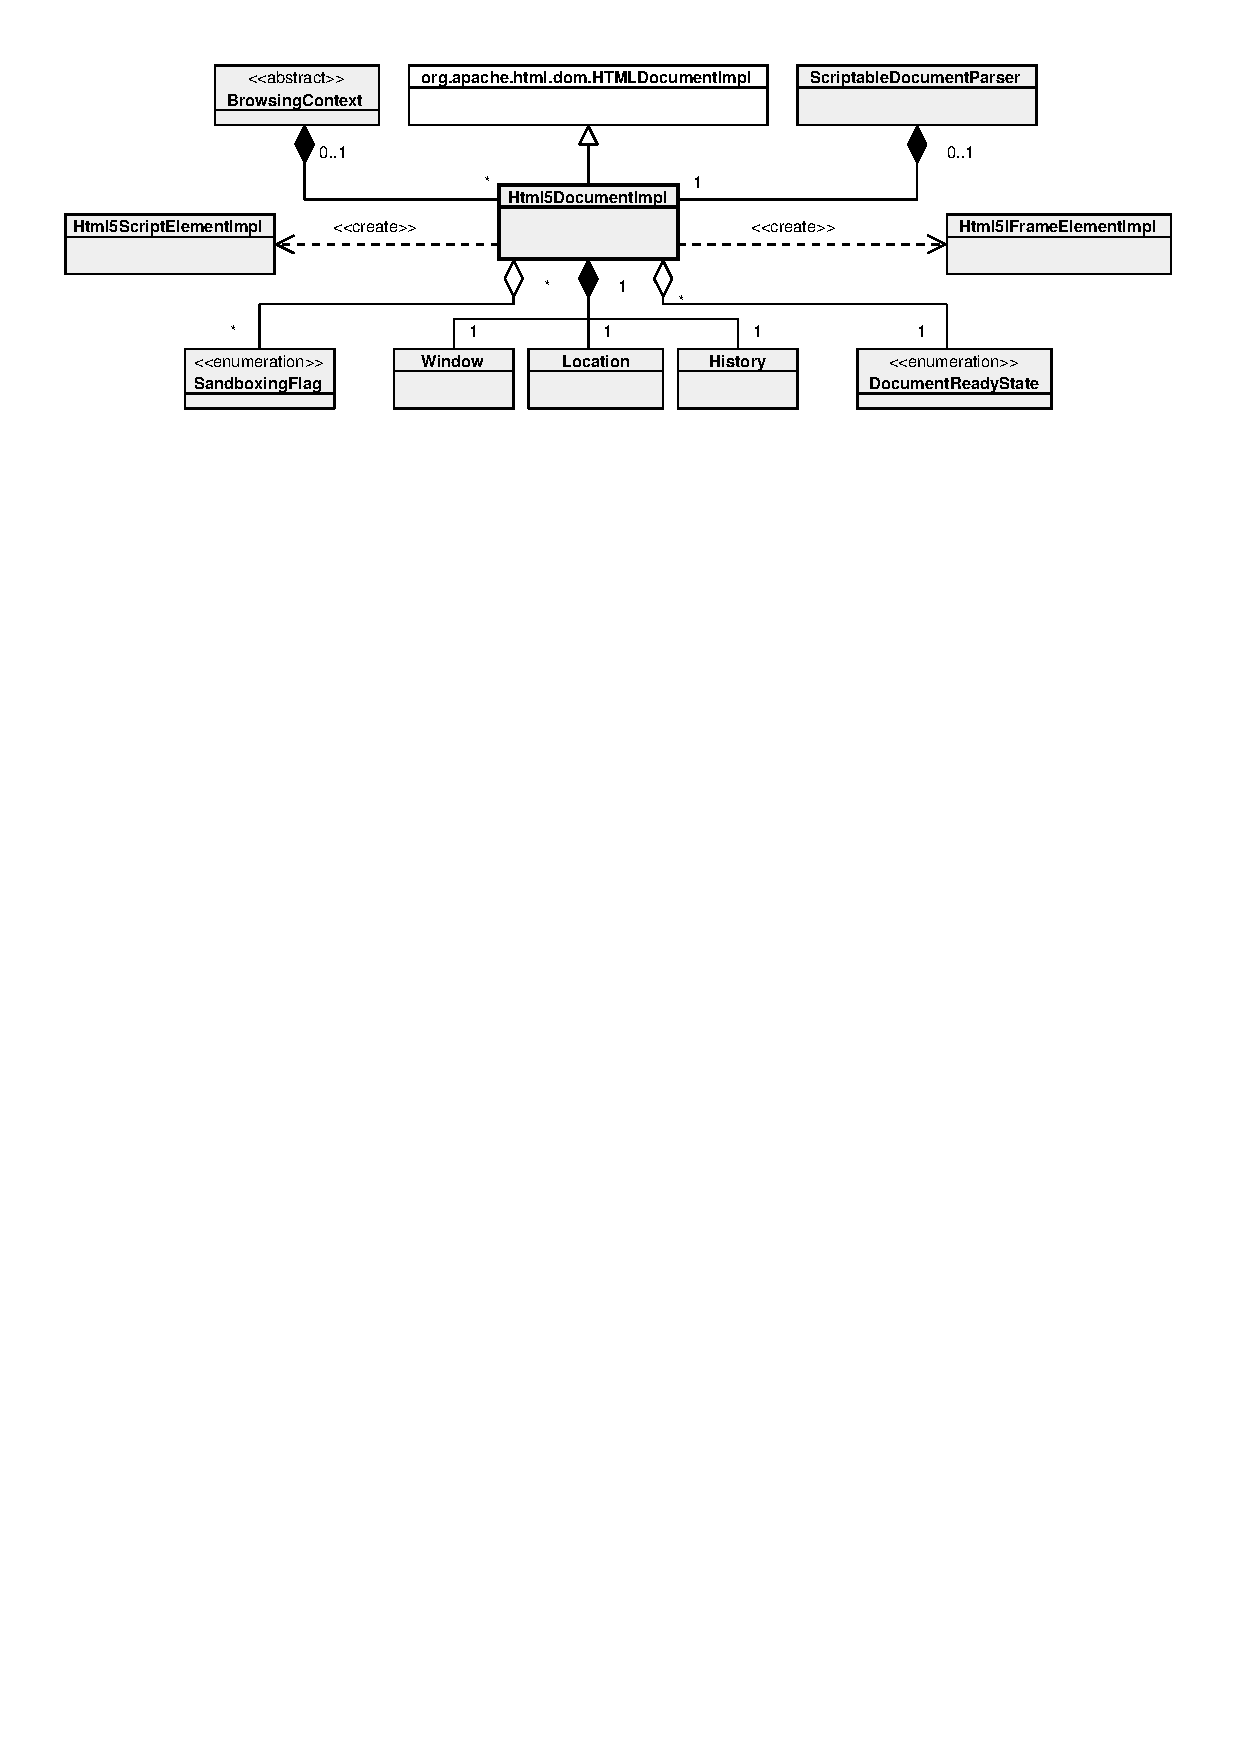
\includegraphics{fig/org-fit-cssbox-scriptbox-dom-Html5DocumentImpl.pdf}
    }
    \caption{Diagram tříd znázorňující třídu dokumentu}
    \label{Figure.DocumentImpl}
  \end{center}
\end{figure}

Dokument dědí z třídy \texttt{HTMLDocumentImpl} knihovny Xerces a~může být asociován s procházecím kontextem nebo parserem, který daný dokument vytvořil. Všechny procházené dokumenty musí mít vždy přidělený procházecí kontext. Zatímco dokument, který byl vytvořen zavoláním metody \texttt{createDocument()} v~rámci provádění skriptu, žádnou referenci na procházecí kontext nevlastní. Stav~dokumentu, ve kterých se může nacházet, je dán atributem výčtu \texttt{DocumentReadyState}:

\begin{itemize}
  \item \textbf{\texttt{LOADING}} -- dokument je načítán parserem;
  \item \textbf{\texttt{INTERACTIVE}} -- parser dokončil dokument, ale stále se čeká na některé zdroje;
  \item \textbf{\texttt{COMPLETE}} -- dokument je zcela kompletně načten.
\end{itemize}

V~dokumentu byly implementovány základní sandbox aspekty. Akce, které sandbox omezuje pro daný dokument, jsou uvedeny množinou sandbox přepínačů \texttt{SandboxingFlag}. 

Během navigace nového dokumentu, jsou nové dokumenty vytvářeny v~rámci zpracovávání obsahu zdroje (kapitola \ref{Chapter.Implementation.ContentHandling}), konkrétně zavoláním statické metody nad dokumentem \texttt{createDocument()}. Během konstrukce dokumentu vznikají nové instance rozhraní \texttt{Location} a~\texttt{History}, které dokument nadále drží ve svém vlastnictví. Pokud byla metoda \texttt{createDocument()} zavolána s recyklovaným dokumentem \texttt{recycleDocument}, je pro nastavení reference objektu \texttt{Window} využit objekt \texttt{Window} recyklovaného dokumentu. Když není recyklovaný dokument nastaven, v~rámci konstrukce se vytváří zcela nová instance objektu \texttt{Window}. Jakmile je nový dokument vytvořen, následuje jeho předání parseru, který zajistí jeho kompletní načtení.

Parser dokumentu představuje třída \texttt{ScriptableDocumentParser} (obrázek \ref{Figure.DocumentParser}). Parsování se vyvolá zavoláním metody \texttt{parse()}, které se předá referenční objekt dokumentu a~vstupní stream s dokumentem. Instance dokumentu není vytvářena parserem, dokument je pouze parserem sestavován a~nikoliv~instanciován. Třída \texttt{ScriptableDocumentParser} reprezentuje vnější rozhraní pro komunikaci s parserem, přičemž parsování neimplementuje. Oddělení od parseru bylo zvoleno z důvodu případné budoucí změny parseru dokumentů na některý jiný, který by více vyhovoval specifikům HTML5. V~současnosti je parsování zajištěno modifikovaným NekoHTML parserem \texttt{ScriptDOMParser}, který přidává podporu pro vytváření vnořených procházecích kontextů pro \texttt{<iframe>} elementy a~spuštění skriptů v~rámci parsování dokumentu, jak to vyplývá z HTML5 specifikace. 

\begin{figure}[H]
  \begin{center}
    \scalebox{0.75}{
      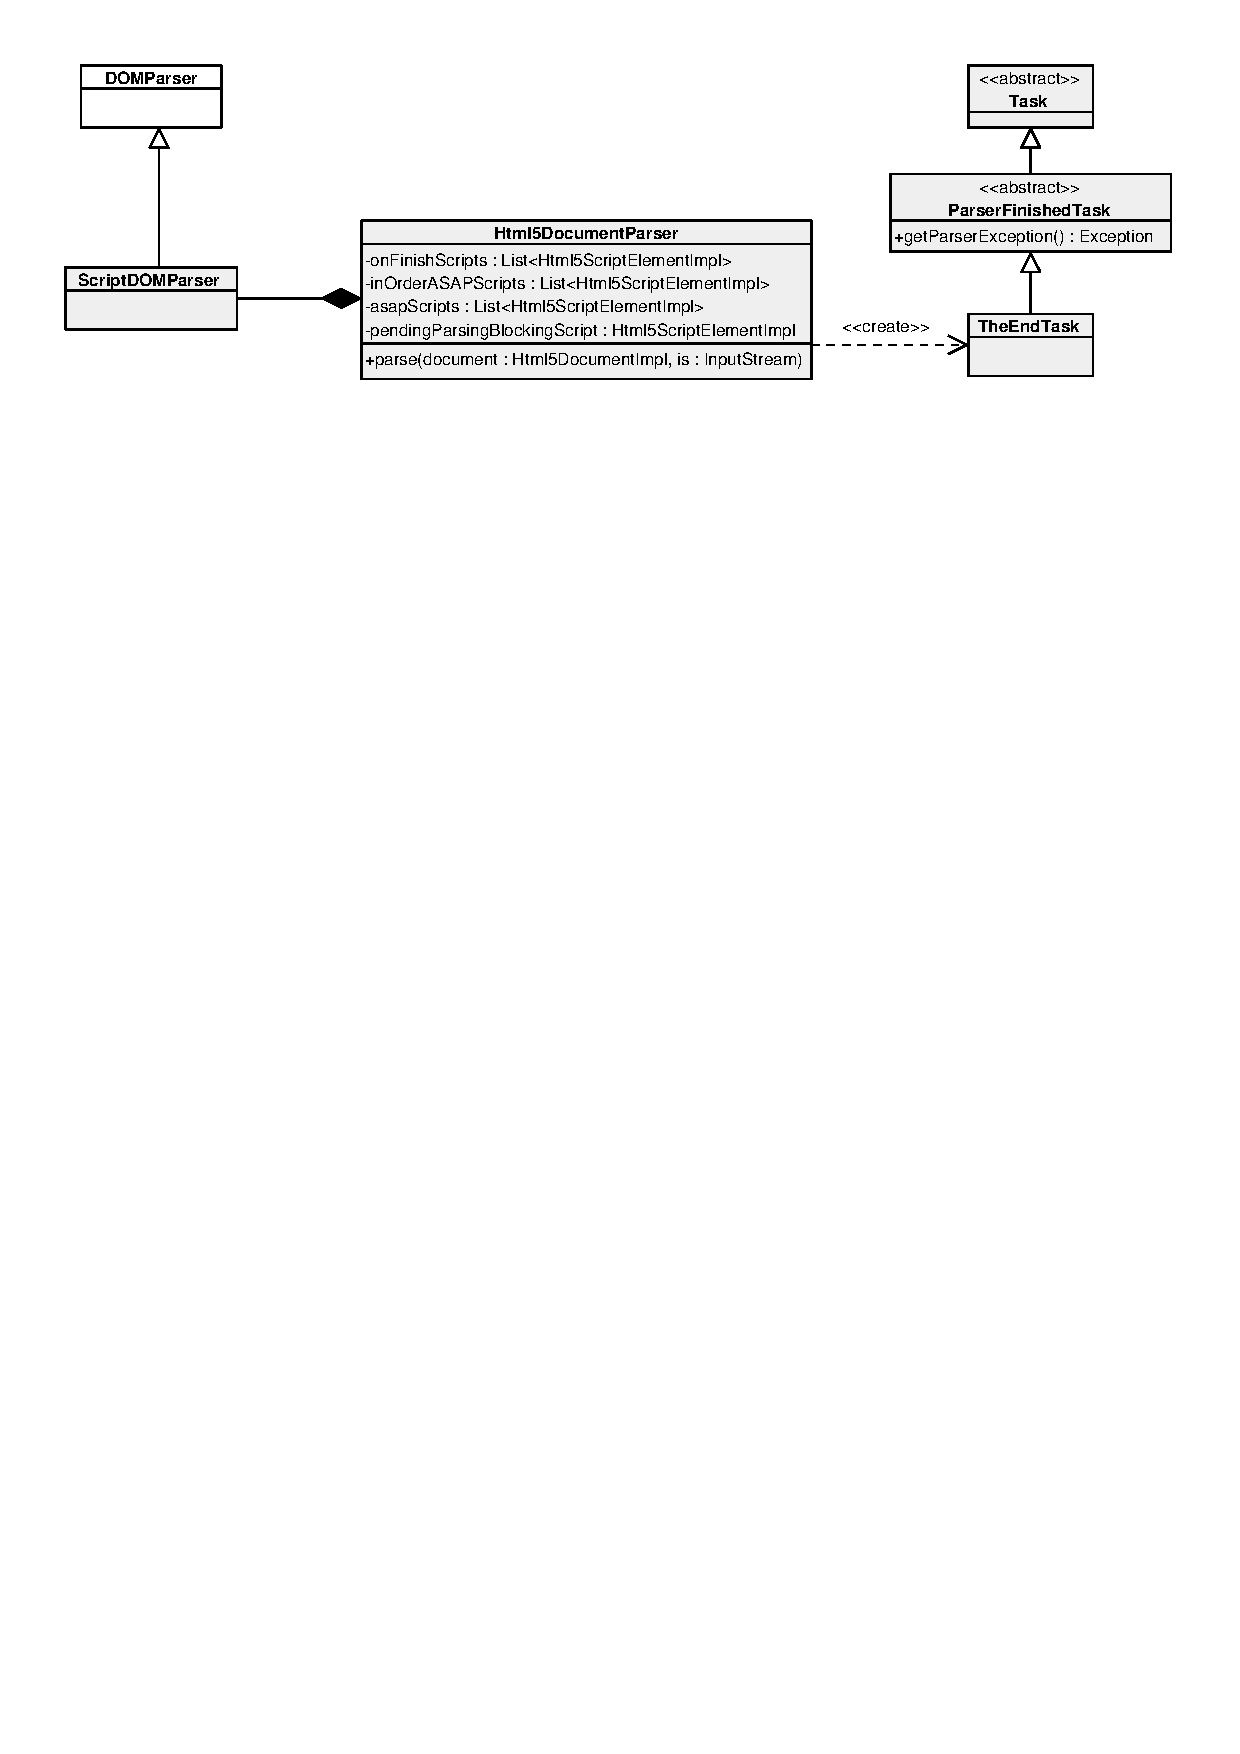
\includegraphics{fig/org-fit-cssbox-scriptbox-parser-Html5DocumentParser.pdf}
    }
    \caption{Diagram tříd znázorňující třídu parseru dokumentu}
    \label{Figure.DocumentParser}
  \end{center}
\end{figure}

Podle specifikace by měl být parser inkrementální a~reentrantní. Měla by být též implementována možnost jeho pozastavení, kde by byl kontext vrácen událostní smyčce na zpracování některé jiné úlohy. Pozastavení parseru je potřeba např. při dokončení parsování skriptu, který by měl být spuštěn v~pořadí , a~při blokování jiným nevykonaným skriptem. Skript může způsobit blokování dalšího skriptu, pokud nebyl stále spuštěn, např. z důvodu, že nebyl dosud stažen ze zdroje. V~této situaci musíme parser pozastavit a~počkat do té doby, dokud není zcela vykonán skript, který byl v~pořadí před právě zpracovaným skriptem. Pozastavení parseru by se obvykle řešilo rotací událostní smyčky. Z důvodu nemožnosti rekonstrukce zásobníku volání NekoHTML parseru bylo pozastavení řešeno vyčleněním parseru do vlastního vlákna a~jeho uspáním.

Třída \texttt{Html5DocumentParser} v~současnosti uchovává referenci na skript, který bude blokovat parsování dokumentu, pokud bude zapotřebí spustit některý další skript v~pořadí. V~třídě jsou také listy skriptů:

\begin{itemize}
  \item \textbf{\texttt{onFinishScripts}} -- skripty, které se mají spustit po dokončení parsování;
  \item \textbf{\texttt{inOrderASAPScripts}} -- skripty k okamžitému spuštění jakmile budou dostupné ve správném pořadí, tak jak byly umístěny v~DOM;
  \item \textbf{\texttt{asapScripts}} -- skripty k okamžitému spuštění jakmile budou dostupné. 
\end{itemize}

Když parser \texttt{ScriptDOMParser} dokončí parsování dokumentu, je vložena do událostní fronty úloha \texttt{TheEndTask}, čímž se navrátí řízení z asynchronního parsování opět událostní smyčce. Úloha nastaví stav~dokumentu na \texttt{INTERACTIVE}, vykoná všechny skripty z~listu \texttt{onFihishScripts}, vyvolá událost \texttt{DOMContentLoaded} nad parsovaným dokumentem a~čeká, dokud nejsou vyprázdněny zbývající listy se skripty -- \texttt{inOrderASAPScripts} a~\texttt{asapScripts}. Po vykonání všech skriptů dojde k nastavení stavu dokumentu na \texttt{COMPLETE} a~vyvolání události \texttt{load} nad daným dokumentem. 

\subsection{Rozhraní Window}
\label{Chapter.Implementation.WindowInterface}

V~kapitole \ref{Chapter.Implementation.DocumentParsing} jsme uvedli interní implementaci dokumentu, která obsahovala instance rozhraní \texttt{History} a~\texttt{Location} -- viditelných rohraní z klientského JavaScriptu. Zatím jsme ovšem nedefinovali, v~rámci jakého rozhraní by měly být viděny právě tyto instance. V~JavaScriptu pro zpřístupnění těchto rozhraní slouží globální objekt \texttt{Window}.

V~implementaci je objekt \texttt{Window} implementován třídou \texttt{Window}. Instance nebo reference v~případě recyklace objektu \texttt{Window} vzniká během konstrukce dokumentu. Implementovaná množina operací a~atributů, s vynecháním atributů uživatelského rozhraní, je znázorněna na obrázku \ref{Figure.WindowInterface}. 

\begin{figure}[H]
  \begin{center}
    \scalebox{0.75}{
      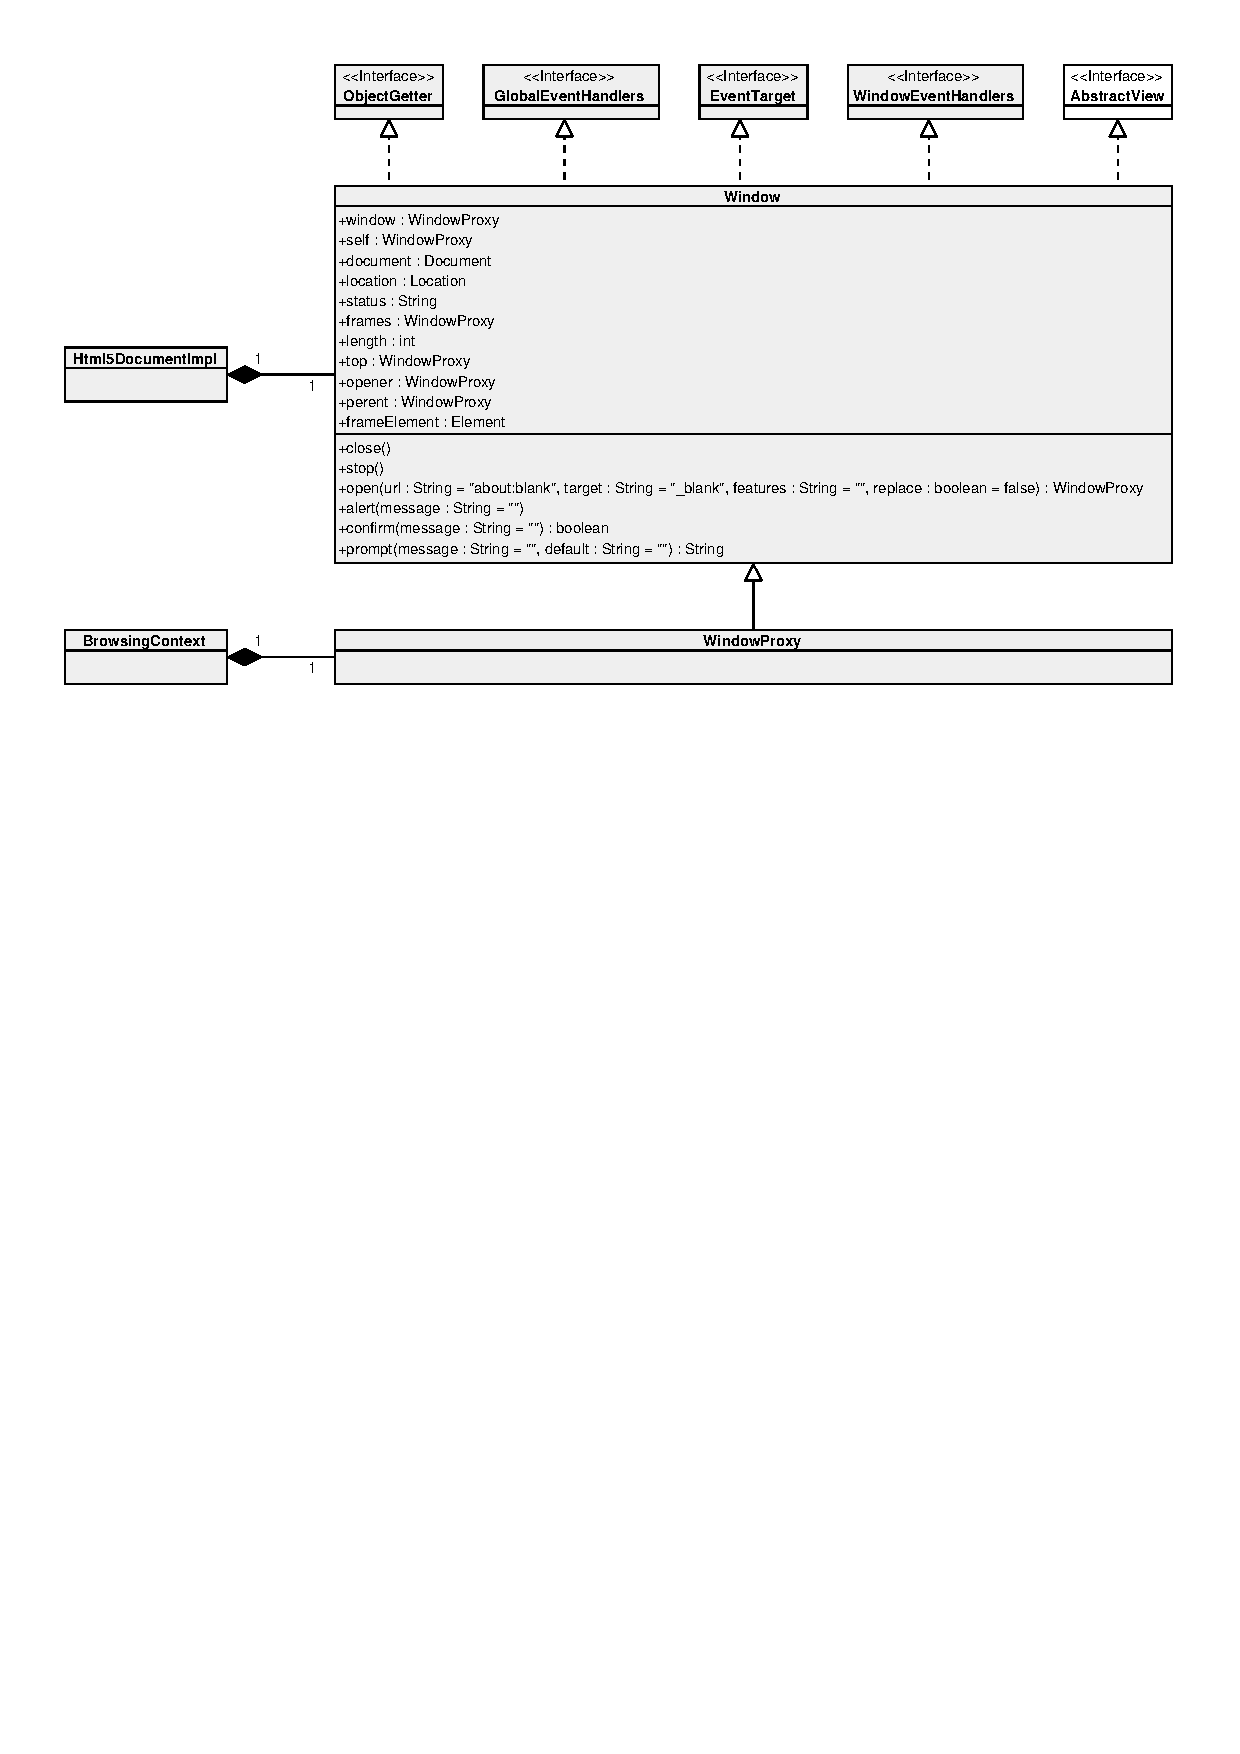
\includegraphics{fig/org-fit-cssbox-scriptbox-window-Window.pdf}
    }
    \caption{Diagram tříd znázorňující rozhraní \texttt{Window}}
    \label{Figure.WindowInterface}
  \end{center}
\end{figure}

Objekt \texttt{Window} využívá plně jádra uživatelského agenta, a~tak jeho implementace je minimální. Atributy \texttt{window}, \texttt{self} a~\texttt{frames} vrací objekt \texttt{WindowProxy} procházecího kontextu dokumentu vlastnícího objekt \texttt{Window}. Atribut \texttt{parent} vrací objekt \texttt{WindowProxy} rodičovského procházecího kontextu a~atribut \texttt{top} objekt \texttt{WindowProxy} kontextu na nejvyšší úrovni. Jedná-li se o objekt \texttt{Window} vnořeného procházecího kontextu, vrací atribut \texttt{frameElement} element, přes který byl tento vnořený procházecí kontext vytvořen. Když je objekt \texttt{Window} vlastněn pomocným procházecím kontextem, atribut \texttt{opener} vrací objekt \texttt{WindowProxy} procházecího kontextu, který pomocný procházecí kontext otevřel. Atributy \texttt{location} a~\texttt{history} přímo vrací aktuální instanci těchto rozhraní z dokumentu, který objekt \texttt{Window} vlastní. Metoda \texttt{close()} ruší procházecí kontext asociovaného dokumentu zavoláním metody \texttt{discard()}. Metoda \texttt{open()} naviguje nové dokumenty s využitím navigačního kontroleru \texttt{NavigationController} procházecího kontextu objektu \texttt{Window}. Metoda \texttt{stop()} ruší všechny požadavky na navigace. Poslední metody pro zobrazení uživatelských dialogů volají korespondující metody v~asociovaném procházecím kontextu. 

V~objektu \texttt{Window} byly kompletně implementovány rozhraní \texttt{GlobalEventHandlers} a~\texttt{WindowEventHandlers}, které přidávají podporu pro snadnou registraci obslužné rutiny pouhým přiřazením callback funkce do atributu bez voláni metody \texttt{addEventListner()}. Objekt \texttt{Window} implementuje také rozhraní \texttt{ObjectGetter}, které slouží pro získávání objektů \texttt{WindowProxy} vnořených procházecích kontextů podle jejich jména nebo indexu. Indexem rozumíme pořadové číslo $0..n$, kde $n$ počet všech procházecích vnořených kontextů určený položkou \texttt{length}.

V~předchozím textu jsme se bavili několikrát o objektu \texttt{WindowProxy}. Tímto objektem myslíme speciální instanci, která má totožné chování jako aktuální globální objekt \texttt{Window} s tím rozdílem, že není asociována pevně s nastaveným dokumentem. Dokument objektu \texttt{WindowProxy} je proměnný v~závislosti na tom, který je právě v~daném procházecím kontextu objektu \texttt{WindowProxy} aktivní. 

\subsection{DOM události}
\label{Chapter.Implementation.DOMEvents}

Všechny uzly objektového modelu dokumentu by měly umožňovat generování událostí. Aby byla tato funkčnost splněna, musí uzly implementovat rozhraní \texttt{EventTarget}. Jelikož dokument \texttt{Html5DocumentImpl} dědí z třídy \texttt{DocumentImpl} knihovny Xerces, nebylo nutno generování událostí pro dokument řešit. Knihovna Xerces totiž rozhraní \texttt{EventTarget} implementuje pro všechny uzly dokumentu. V~klientském JavaScriptu ovšem není kořenem DOMu samotný dokument, jak je implementováno v~Xerces, nýbrž objekt \texttt{Window}. Z tohoto důvodu bylo zapotřebí řešit provázání s objektem \texttt{Window} a~generování událostí i do nového kořenového objektu, jak je znázorněno na obrázku \ref{Figure.EventWindowDocument}. 

\begin{figure}[H]
  \begin{center}
    \scalebox{0.45}{
      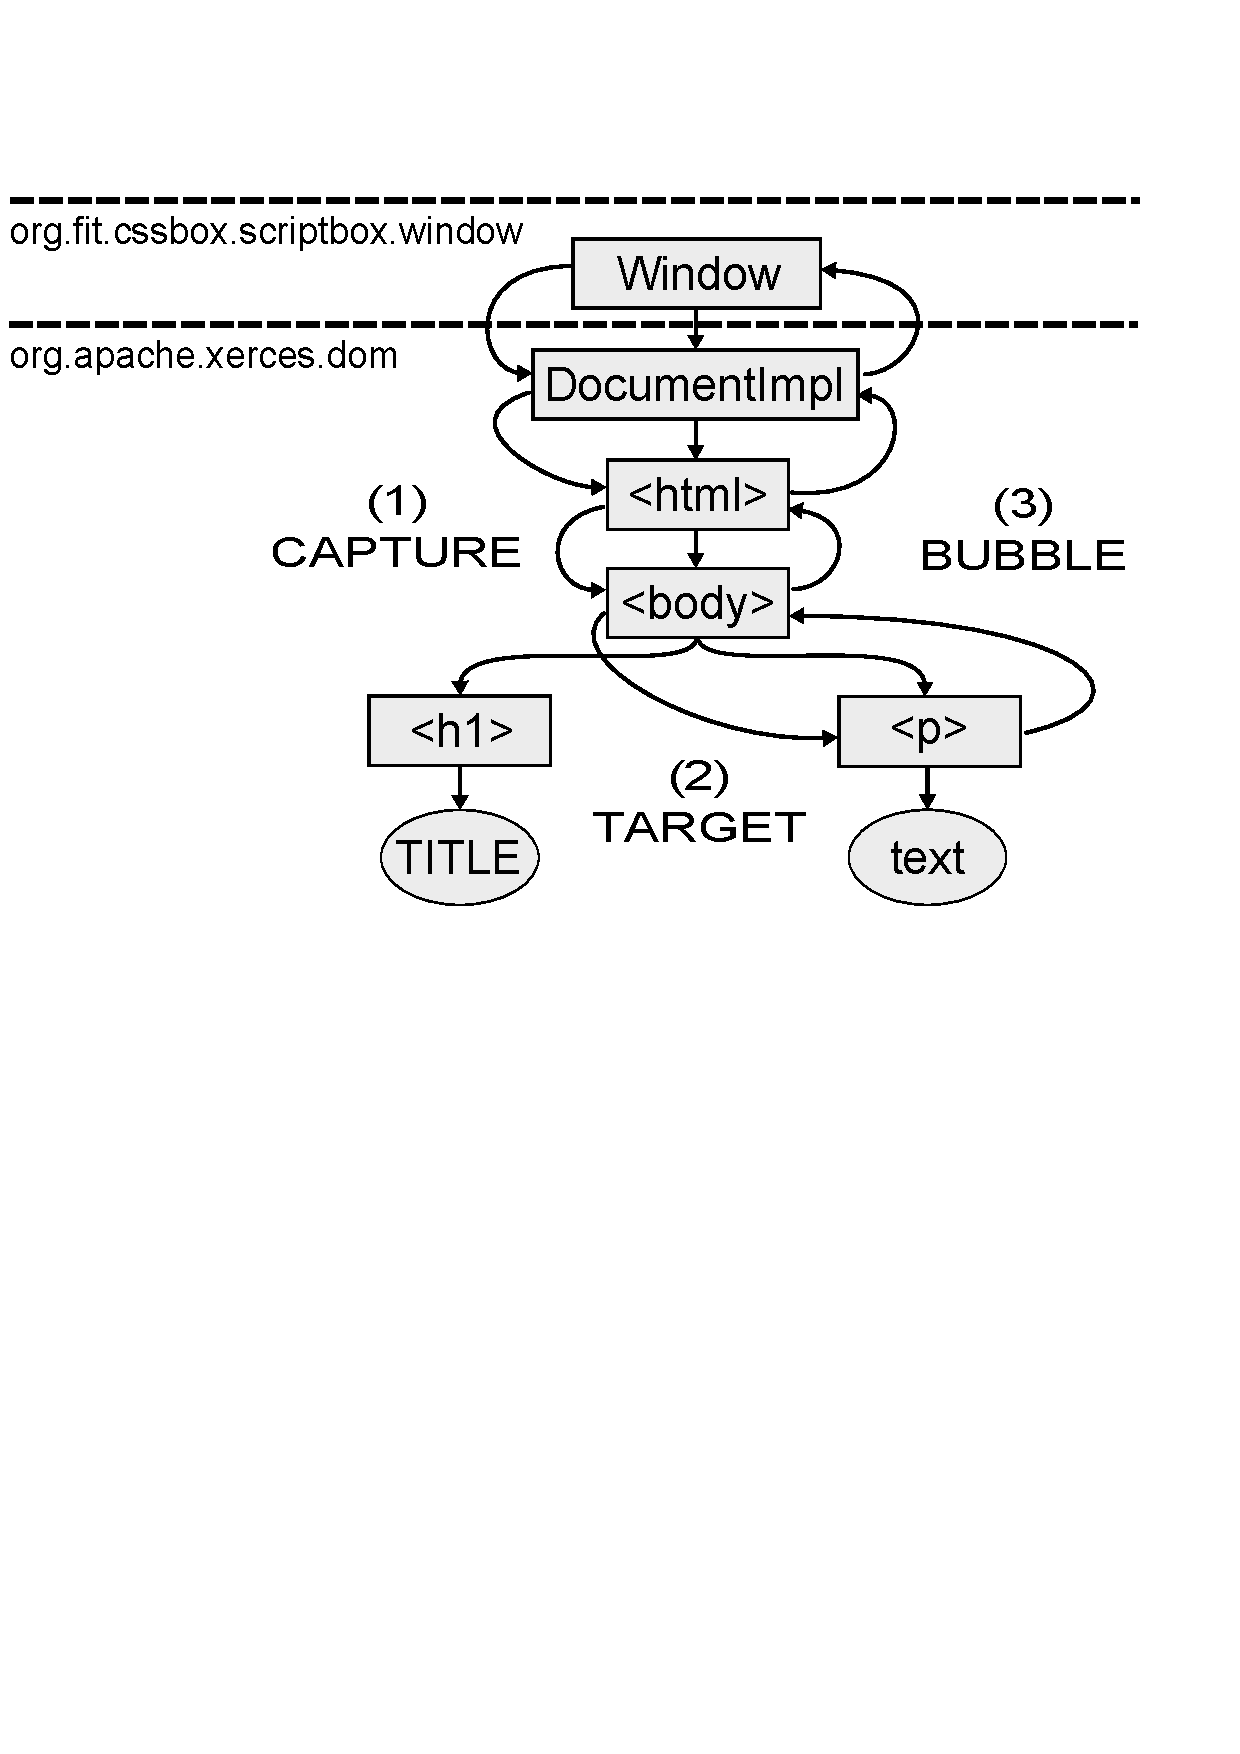
\includegraphics{fig/events.pdf}
    }
    \caption{Ilustrace toku události z objektu \texttt{Window} do objektu dokumentu}
    \label{Figure.EventWindowDocument}
  \end{center}
\end{figure}

Události se generují zavoláním metody \texttt{dispatchEvent()} rozhraní \texttt{EventTarget} nad jakýmkoliv~uzlem, který toto rozhraní implementuje. V~implementaci Xerces jsou všechny události, které jsou předány metodě \texttt{dispatchEvent()}, dále delegovány chráněné metodě dokumentu \texttt{dispatchEvent()}, která požadované generování událostí implementuje. Jednotné místo v~dokumentu pro generování událostí umožnilo snadnou změnu mechanismu generování událostí. Po provedené úpravě se dokument chová tak, jakoby byl kořenovým uzlem pro generování událostí objekt \texttt{Window}.

Během generování událostí v~přizpůsobeném modelu mohou nyní nastat dvě situace. První situace je, pokud bylo zavoláno \texttt{dispatchEvent()} nad objektem \texttt{Window}. V~tomto momentě se okamžitě volají všichni zaregistrovaní odběratelé dané události, přičemž fáze \texttt{CAPTURE} a~\texttt{BUBBLE} se neprovádí, jelikož se jedná o kořenový uzel. Druhá situace již obnáší změnu zmíněné chráněné metody \texttt{dispatchEvent()}. Situace vzniká po zavolání metody \texttt{dispatchEvent()} nad některým uzlem dokumentu. V~tomto případě se provádí následující kroky:

\begin{enumerate}
  \item Zavolání metody \texttt{dispatchEventFromDocument()} nad objektem \texttt{Window}, ve které se obslouží \texttt{CAPTURE} fáze. 
  \item Zavolání původní implementace \texttt{dispatchEvent()}, která zajistí propagaci události až do daného cíle a~její návrat zpět do dokumentu. 
  \item Opětovné zavolání \texttt{dispatchEventFromDocument()} pro obsloužení \texttt{BUBBLE} fáze.
\end{enumerate}

Elementy DOMu, ale i objekt \texttt{Window} v~klientském JavaScriptu neimplementují pouze rozhraní \texttt{EventTarget}, ale přidávají i vhodně pojmenované atributy, jejichž setter zajistí registraci nastavené událostní obslužné rutiny jako odběratele v~daném objektu. Elementy implementují množinu atributů událostních obslužných rutin \texttt{GlobalEventHandlers}. Objekt \texttt{Window} implementuje dále rozhraní \texttt{WindowEventHandlers}.

Událostní obslužné rutiny musí v~programu implementovat \texttt{EventHandler}, který jako rozhraní \texttt{EventListener} obsahuje pouze jednu metodu pro obsloužení dané události. Při nastavování obslužných rutin do korespondujících atributů událostních obslužných rutin rozhraní \texttt{GlobalEventHandlers} nebo \texttt{WindowEventHandlers} musela být řešena odregistrace odběratele staré obslužné rutiny a~registrace nového odběratele nové obslužné rutiny. Za tímto účelem byla vytvořena třída \texttt{EventHandlerEventListener}, která registruje a~odebírá událostní obslužné rutiny u cíle implementujícího \texttt{EventTarget} (obrázek \ref{Figure.EventHandlerEventListener}).

\begin{figure}[H]
  \begin{center}
    \scalebox{0.75}{
      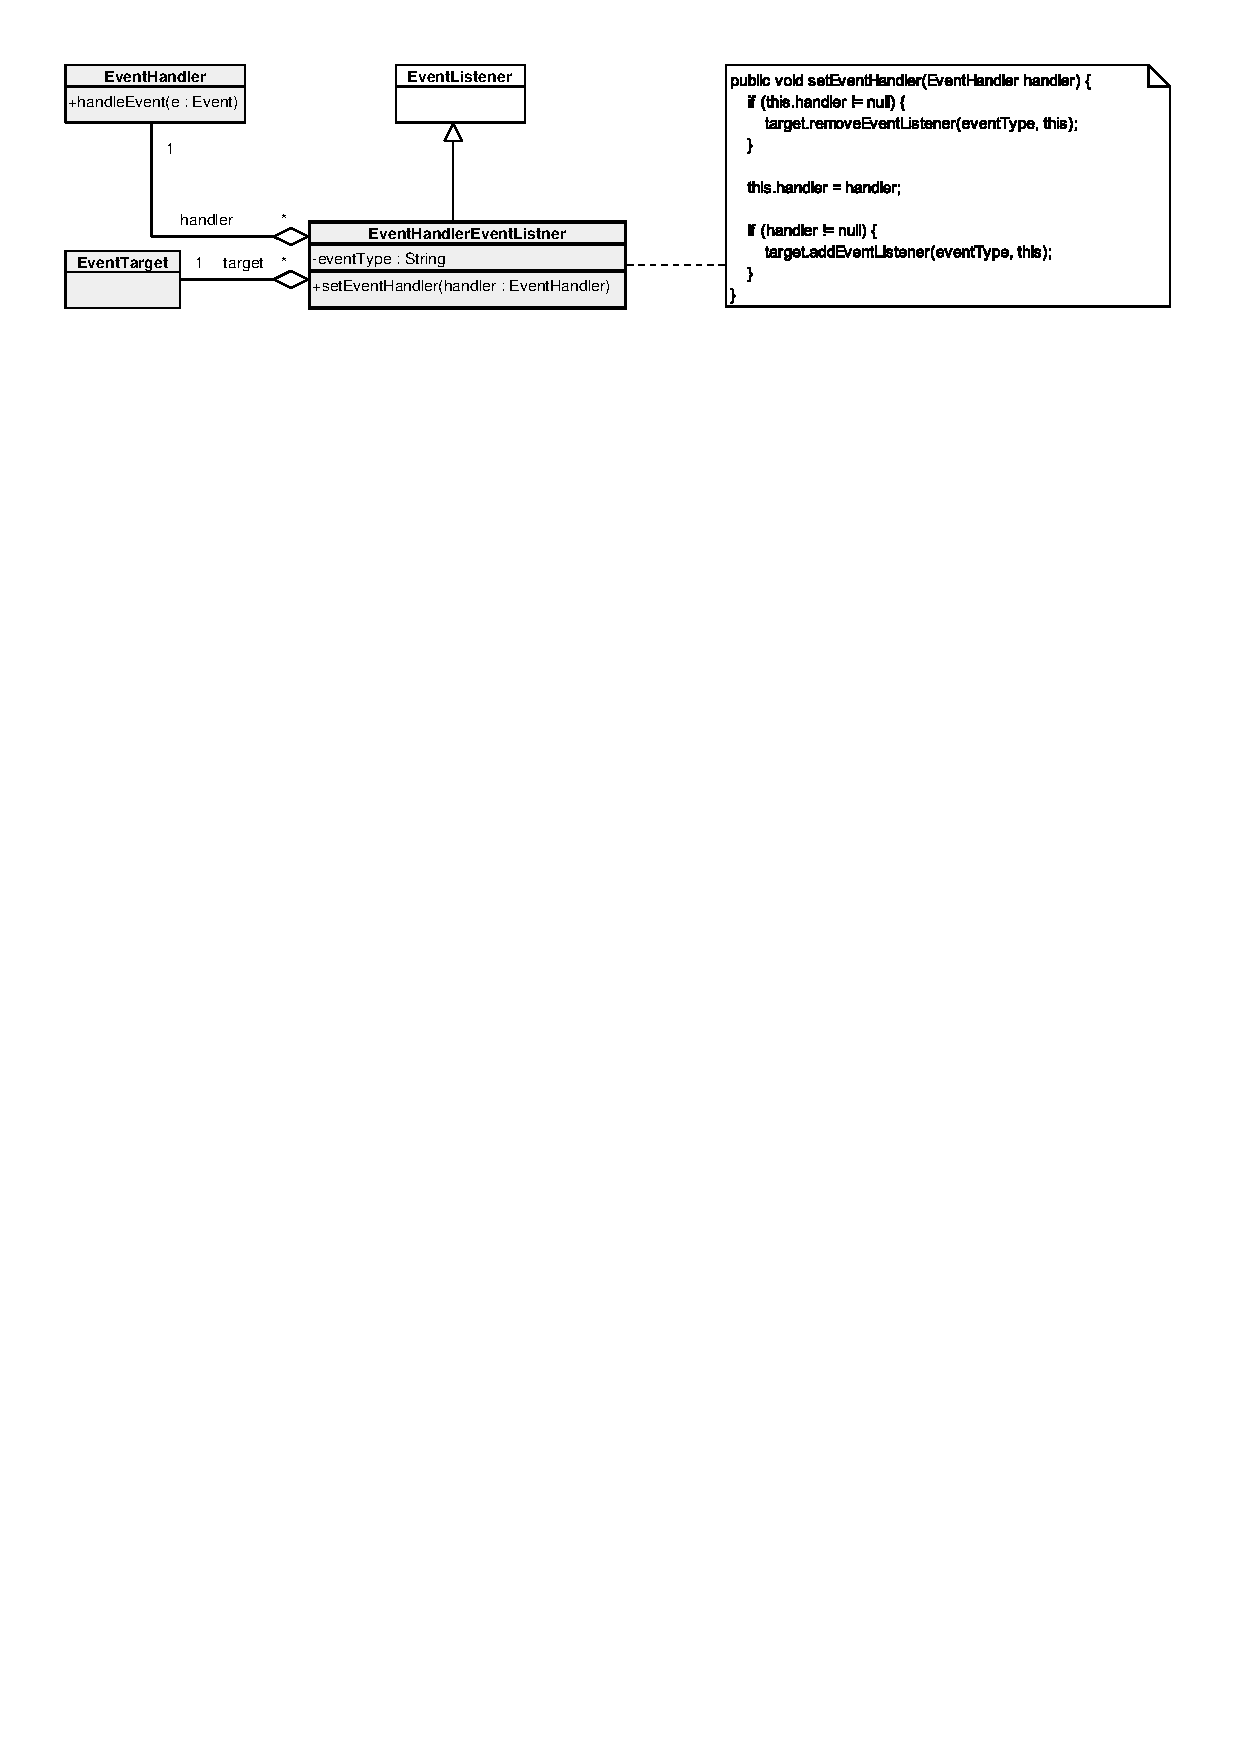
\includegraphics{fig/org-fit-cssbox-scriptbox-dom-events-EventHandlerEventListener.pdf}
    }
    \caption{Diagram tříd znázorňující registrování objektu \texttt{EventHandler}}
    \label{Figure.EventHandlerEventListener}
  \end{center}
\end{figure}

\vspace{-1em}

\noindent V~současnosti jsou jádrem prohlížeče generovány události uvedené v~následující tabulce \ref{Table.SupportedEvents}.

\smallskip

\begin{table}[H]
  \begin{center} 
    \begin{tabular}{|l|p{5cm}|P{6cm}|} \hline
    \theadStart{Třída události} & \thead{Popis třídy} & \thead{Typy událostí} \\ \hline
    \texttt{Event} & jednoduché události neobsahující žádné další informace kromě názvu události & \texttt{load}, \texttt{beforescriptexecute}, \mbox{\texttt{unload}}, \texttt{afterscriptexecute}, \texttt{abort}, \texttt{DOMContentLoaded} \\ \hline
    \texttt{PopStateEvent} & událost změny uloženého stavu ve společné historii sezení & \texttt{popstate} \\ \hline
    \texttt{HashChangeEvent} & událost změny fragmentu v~URL prohlížené stránky & \texttt{hashchange} \\ \hline
    \texttt{ErrorEvent} & událost reprezentující chybu & \texttt{error} \\ \hline
    \texttt{MouseEvent} & události vyvolané ukazatelem myši & \texttt{mouseover}, \texttt{mousedown}, \texttt{mouseup}, \texttt{click}, \texttt{dblclick} \\ \hline
    \end{tabular}
    \caption{Třídy podporovaných událostí}
    \label{Table.SupportedEvents}
  \end{center}
\end{table}

\subsection{Rozhraní URLUtils a~URL}
\label{Chapter.Implementation.URLUtilsInterface}

Pro zkompletování výkladu všech rozhraní, která jsou v~současné implementaci viditelná z klientského JavaScriptu nám chybí uvést poslední rozhraní \texttt{URL}, jež čerpá z dalšího rozhraní \texttt{URLUtils}. Rozhraní \texttt{URLUtils} není použité pouze pro objekty \texttt{URL}, ale i pro objekt implementující rozhraní \texttt{Location}. Ve své implementaci \texttt{URLUtils} rozhraní obaluje vstupní řetězec s URL adresou -- \texttt{input}, který dále vnitřně parsuje za pomocí parseru \texttt{URLParser}, čímž vzniká objekt url třídy \texttt{ParserURL} (obrázek \ref{Figure.URLInterface}). Zpracovaná adresa \texttt{ParserURL} poskytuje náležitými gettery možnost získávání jednotlivých komponent URL adresy, které jsou přístupné právě přes rozhraní \texttt{URLUtils}. 

\begin{figure}[H]
  \begin{center}
    \scalebox{0.75}{
      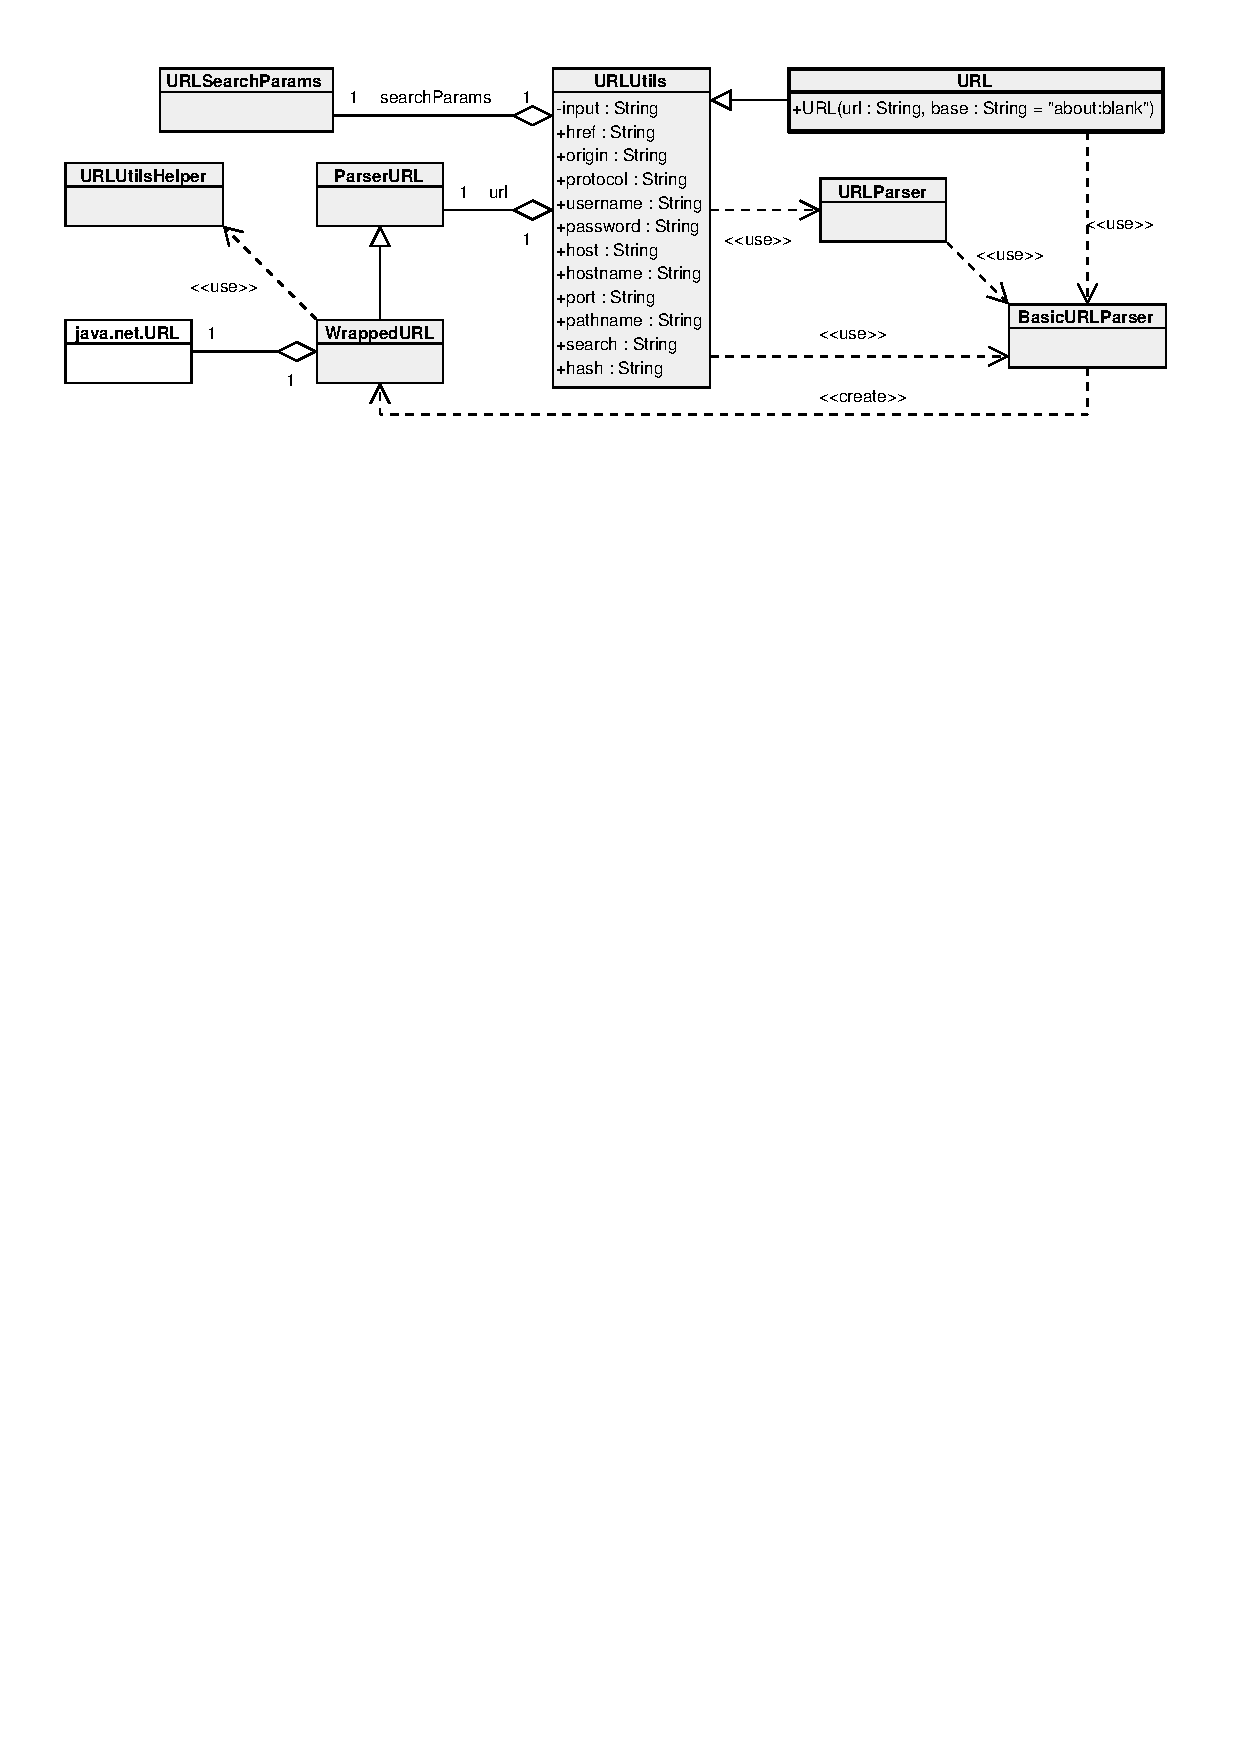
\includegraphics{fig/org-fit-cssbox-scriptbox-url-URL.pdf}
    }
    \caption{Diagram tříd znázorňující implementované rozhraní URL}
    \label{Figure.URLInterface}
  \end{center}
\end{figure}

Parser \texttt{ParserURL} vnitřně používá \texttt{BasicURLParser}, který zajišťuje náležité parsování předaného URL řetězce. Jelikož tvorba parseru nebyla cílem této práce, \texttt{BasicURLParser} nevytváří nový objekt \texttt{ParserURL} podle referenčního algoritmu tak, jak bylo uvedeno ve specifikaci. BasicURLParser pouze využívá již implementovaného parsovacího mechanismu v~balíku \texttt{java.net} a~třídy \texttt{URL}, jejíž objekt parsováním vznikne. Objekt třídy \texttt{URL} se obaluje do rozhraní \texttt{ParserURL}, což je zajištěno adaptující třídou \texttt{WrappedURL}.

Rozhraní \texttt{URL} vůči rozhraní \texttt{URLUtils} nepřidává žádnou další funkcionalitu, ale pouze definuje konstruktor pro tvorbu URL adresy, kterou objekt zapouzdřuje.

\section{Scriptovací architektura pro dokumenty}
\label{Chapter.Implementation.ScriptingArchitecture}

Do HTML dokumentů mohou být vkládány klientské skripty různých skriptovacích jazyků dle rozebrané problematiky v~návrhu -- kapitole \ref{Chapter.Design}. Abychom umožnili snadnou implementaci klientských skriptovacích enginů pro různé skriptovací enginy, bylo nutné vytvořit základní abstraktní architekturu, která bude pro všechny skriptovací enginy společná. 

V~této kapitole popíšeme implementaci abstraktního skriptovacího enginu a~architekturu vytváření nativních objektů Javy tak, aby mohly být exportovány do skriptů. Fundamentální skriptovací architektura se nachází v~balíku \texttt{org.fit.cssbox.scriptbox.script}. 

Architektura pro skriptací enginy vychází z kapitoly návrhu. Architektura byla v~některých problematických částech mírně upravena tak, aby věrohodně kopírovala specifikaci HTML 5. Nejzásadnější změnou vůči návrhu je způsob spouštění skriptů. Skripty nejsou spouštěny pomocí jednotné třídy \texttt{DocumentScriptEngine}, která eviduje všechny skriptovací enginy, asociuje je pro dané dokumenty a~implementuje veškerou funkcionalitu pro jejich spouštění. Z důvodu prevence proti případné nekompatibilitě s danou specifikací, umožnění její snadnější a~přesnější interpretace, bylo implementováno decentralizované spouštění skriptů. Odkaz na skriptovací engine nyní není vlastněn globální instancí spravující třídy \texttt{DocumentScriptEngine}, ale dokumentem samotným v objektu \texttt{ScriptSettings}.

Implementované řešení provádění skriptů v~dokumentu a~objekt \texttt{ScriptSettings} je popsán v~kapitole \ref{Chapter.Implementation.ScriptInterface}. Injekce objektů do hlavního scopu (kapitola \ref{Chapter.Design.GlobalScopeInjections}) byla zcela implementována bez odlišností od návrhu, je rozebrána v~kapitole \ref{Chapter.Implementation.OtherFunctionality}. Tvorba JavaScriptového enginu podle JSR 223 (kapitola \ref{Chapter.Design.JavaScriptEngineJSR223}) byla též kompletně dodržena. Rhino engine byl v~mnoha ohledech přizpůsoben a~vylepšen tak, aby ho bylo možné využít pro klientské skripty. O~implementovaném řešení JavaScript enginu pojednává kapitola \ref{Chapter.Implementation.ScriptEngines}.

\subsection{Rozhraní skriptů dokumentu}
\label{Chapter.Implementation.ScriptInterface}

Podle specifikace HTML5 bylo zapotřebí implementovat společné rozhraní pro skripty dokumentu. Rozhraní pro skripty je v~implementaci reprezentováno abstraktní třídou \texttt{Script}. Každý skript využívá pro svoji tvorbu a~běh určitého nastavení daného abstraktní třídou \texttt{ScriptSettings}. 

\begin{figure}[H]
  \begin{center}
    \scalebox{0.80}{
      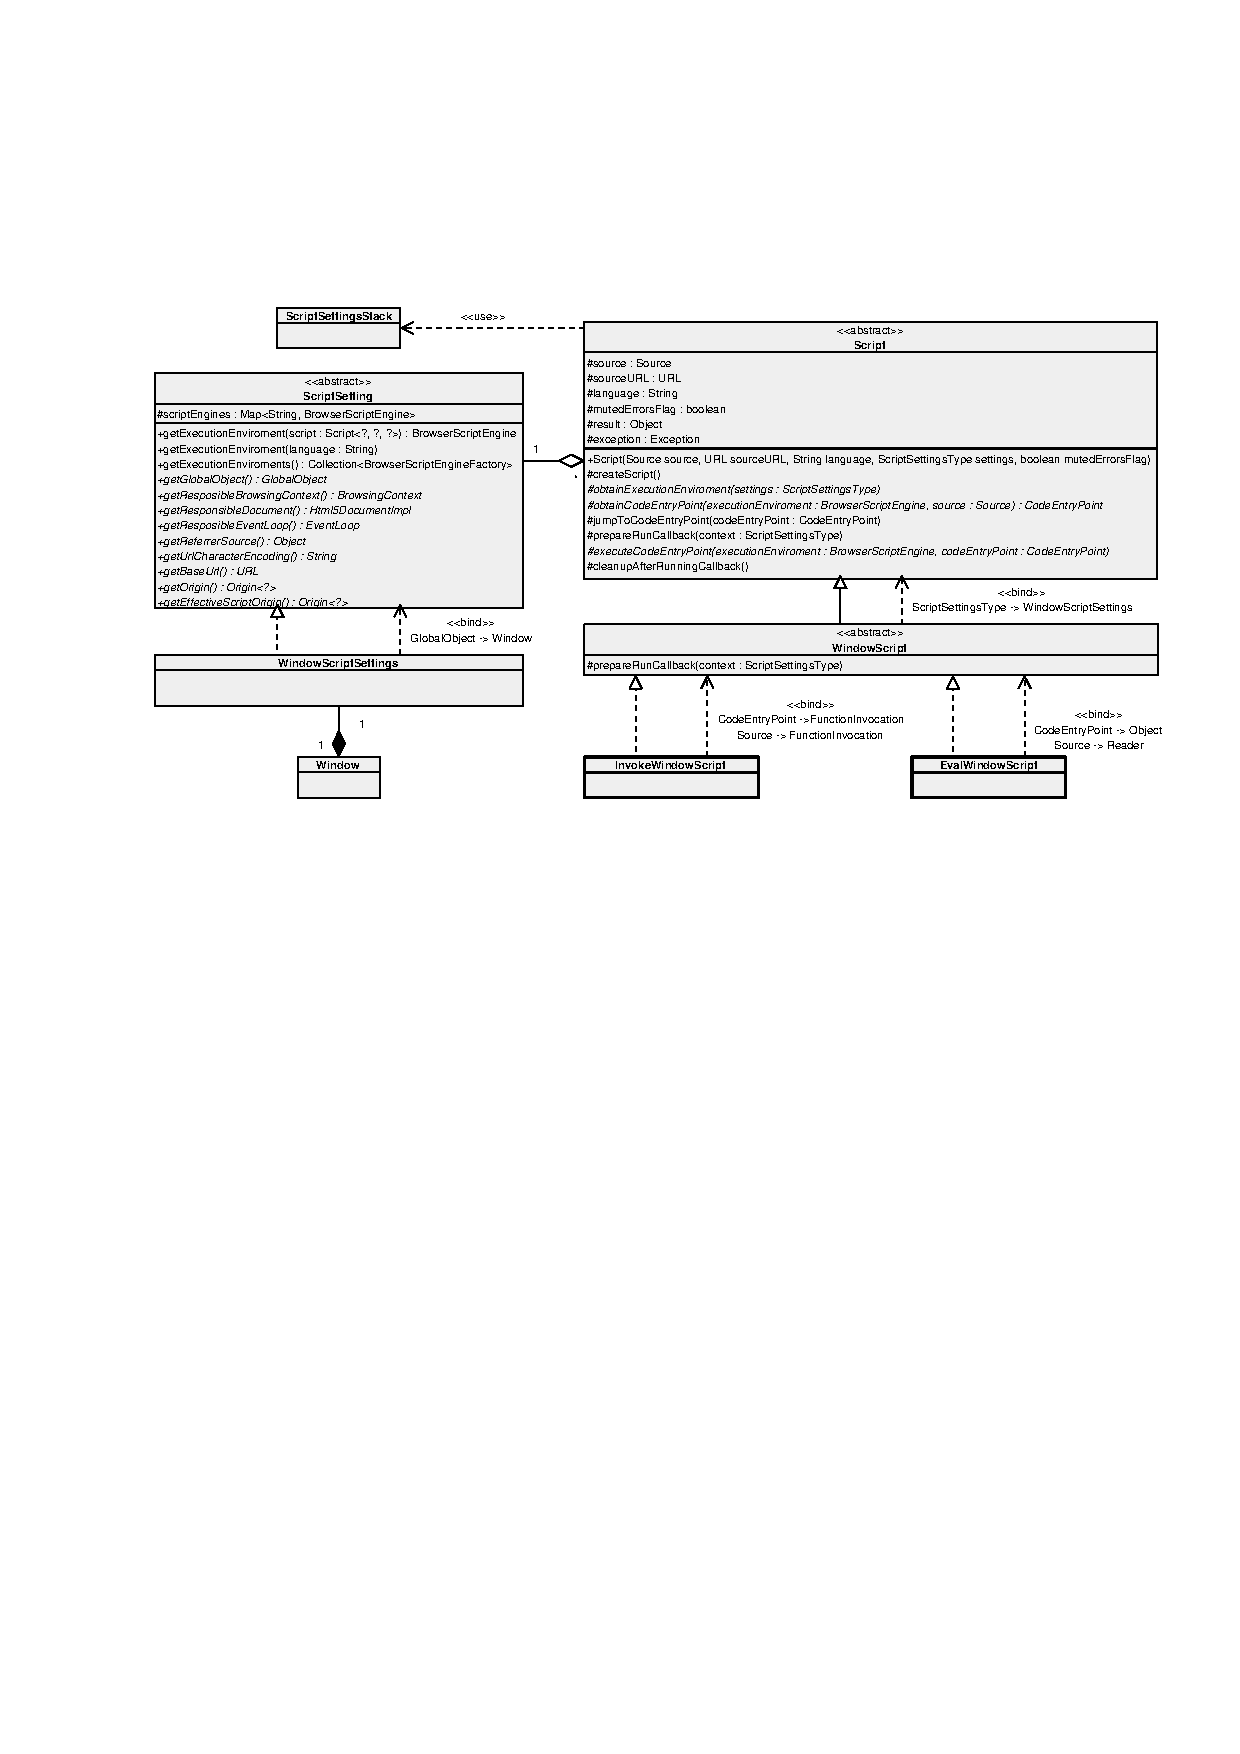
\includegraphics{fig/org-fit-cssbox-scriptbox-script-Script.pdf}
    }
    \caption{Diagram tříd znázorňující implementované rozhraní skriptu}
    \label{Figure.ScriptInterface}
  \end{center}
\end{figure}

Nastavení pro skripty deklaruje důležité aspekty prostředí, ve kterém by se měl skript vykonat. Třída \texttt{ScriptSettings} je abstraktní a~v~současné implementaci ji realizuje jediná třída \texttt{WindowScriptSettings}. Instance nastavení je vytvářena vždy během konstrukce objektu \texttt{Window}, který je zároveň globálním objektem pro JavaScriptový engine. Třída skriptu \texttt{WindowScriptEngine} poskytuje referenci zejména na:

\begin{itemize}
  \item dokument \texttt{Html5DocumentImpl}, ve kterém se nachází spuštěný skript;
  \item globální objekt \texttt{Window};
  \item bázovou URL adresu, která bude použita pro vytváření URL adres z adres relativních;
  \item událostní smyčku \texttt{EventLoop} určenou pro skripty
  \item původ skriptu \texttt{Origin}, jeho kódování, atd. 
\end{itemize}

Jelikož nastavení pro skripty je unikátní pro každý objekt Window, který je přímo v~$1:1$ asociaci s objektem dokumentu, bylo nastavení využito pro tvorbu a~uchovávání skriptovacích enginů dokumentu. Skriptovací enginy lze vytvářet zavoláním metody nastavení skriptu \texttt{getExecutionEnviroment()}. Jakmile je skriptovací engine již jednou vytvořen, je v~konkrétním nastavení uchován a~během příštího dotazu opět navrácen. Při vytváření neustále nových skriptovacích enginů by docházelo ke ztrátě uchovaného kontextu uvnitř enginů.

Abstraktní třída pro skripty \texttt{Script} potřebuje pro svoji konstrukci zdroj skriptu \texttt{Source}, jazyk skriptu, URL ze které byl případně skript získán a nastavení pro skripty generického typu \texttt{ScriptSettingsType}. V~rámci tvorby instance skriptu se skript ihned provede zavoláním chráněné metody \texttt{createScript()}. Způsob spuštění skriptu je znázorněn na obrázku \ref{Figure.CreateScript}. Jakmile se ověří, zda je skriptování povoleno, dojde nejprve k získání skriptovacího enginu metodou \texttt{obtainExecutionEnviroment()}. Pak dojde k přípravě skriptu a~získání vstupního bodu k vykonání \texttt{CondeEntryPoint} metodou \texttt{obtainCodeEntryPoint()}, který je vykonán metodou \texttt{jumpToCodeEntryPoint()}. Vykonávací metoda před spuštěním skriptu vkládá před spuštěním skriptu na zásobník \texttt{ScriptSettingsStack} aktuální nastavení skriptu, jež je po skončení vykonávání opět ze zásobníku odstraněno. Zásobník skriptů je potřebný v~některých situacích, např. když chceme znát některé základní informace o nastavení skriptu, který spustil některou funkci jádra uživatelského agenta. Během navigování stránek metodou \texttt{open()} objektu Window se využívá zásobníku k určení zdrojového procházecího kontextu, který je totožný s responsivním procházecím kontextem skriptu.

\begin{figure}[H]
  \begin{center}
    \scalebox{0.75}{
      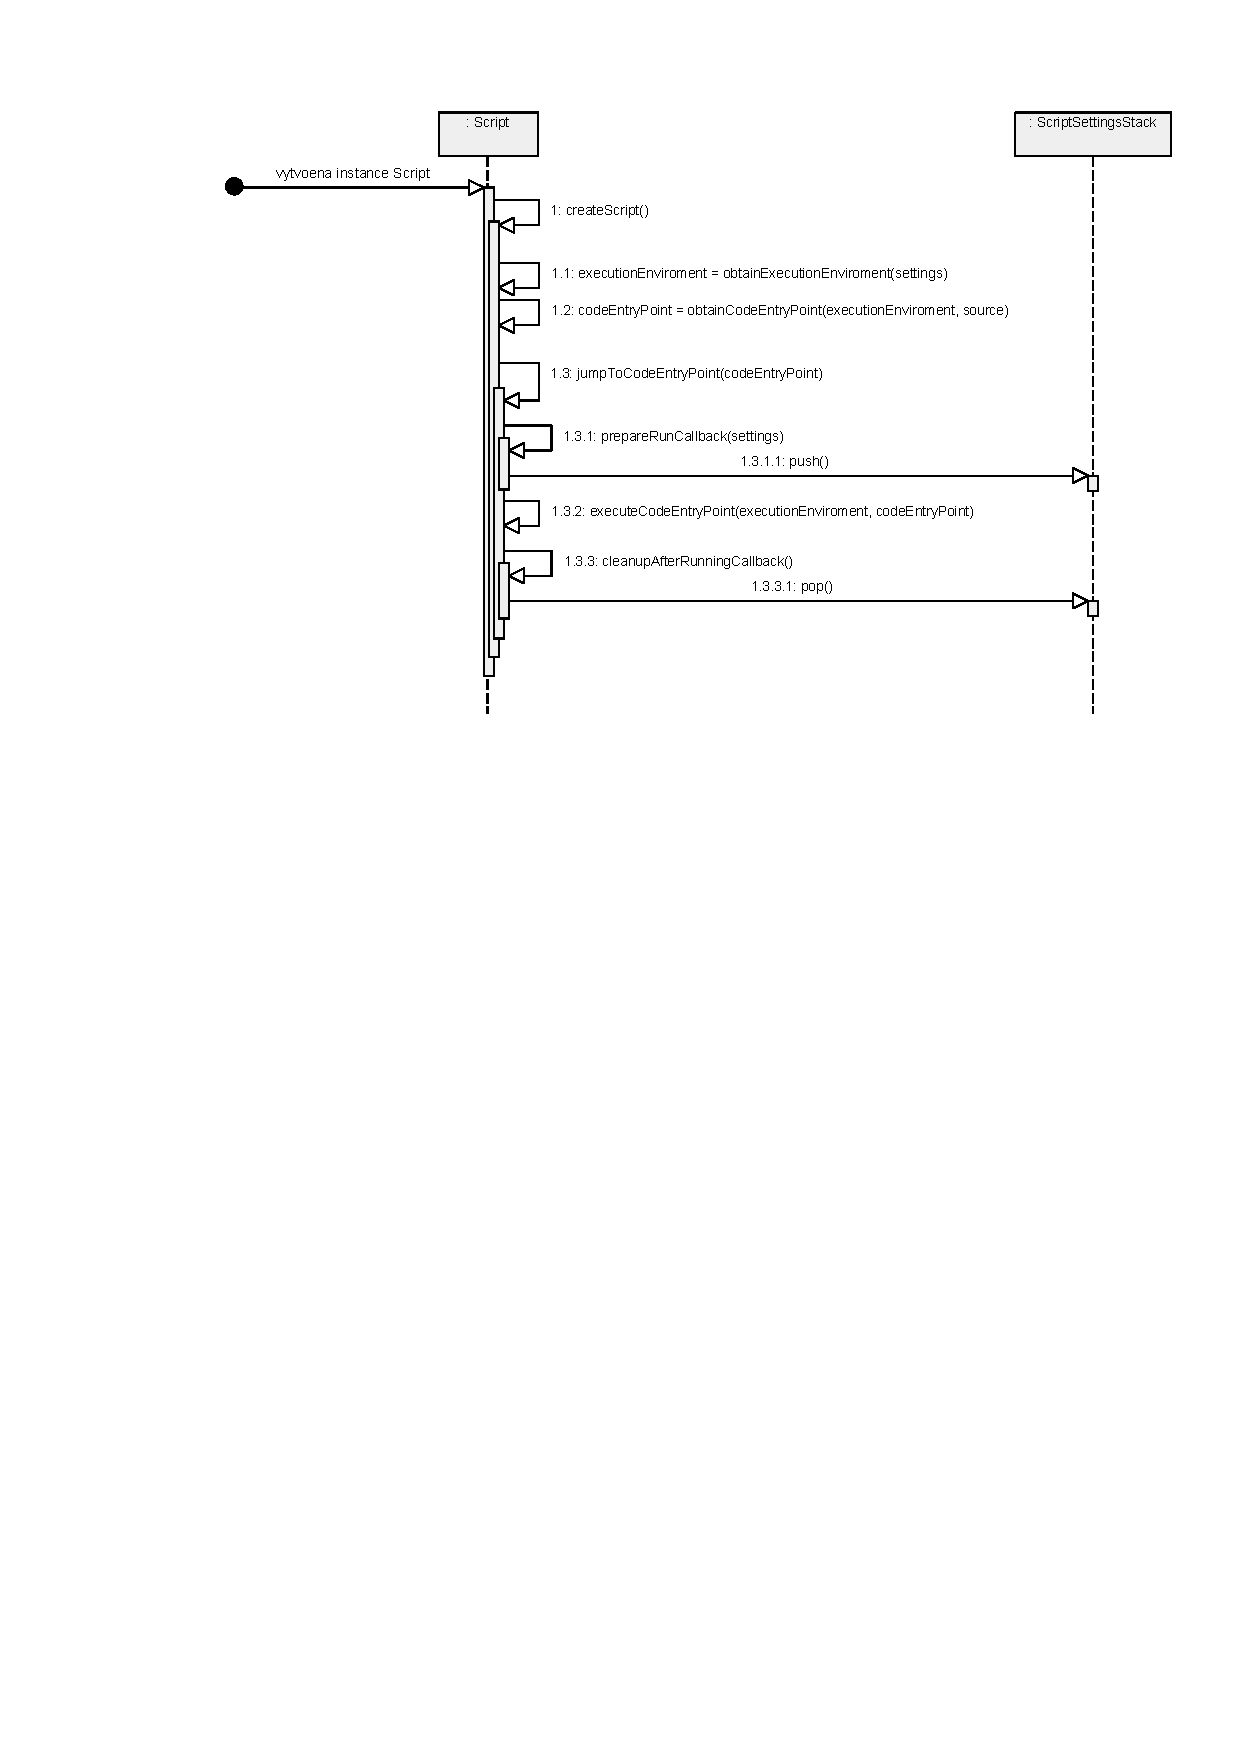
\includegraphics{fig/create-script.pdf}
    }
    \caption{Sekvenční diagram znázorňující tvorbu skriptu}
    \label{Figure.CreateScript}
  \end{center}
\end{figure}

\vspace{-1em}

Jedinými konkrétními třídami abstraktní třídy \texttt{Script} jsou třídy \texttt{EvalWindowScript} a~\texttt{InvokeWindowScript}. Obě zmíněné třídy rozšiřují třídu \texttt{WindowScript}, jež předefinovává metodu \texttt{prepareRunCallback()}, do které přidává test, zda je dokument objektu \texttt{Window} plně aktivní. Pokud není dokument aktivní, vrací metoda nepravdu a~skript není spuštěn.

Třída \texttt{EvalWindowScript} slouží k prostému vykonávání spustitelného kódu v~nalezeném skriptovacím enginu. Zdrojem pro skripty \texttt{EvalWindowScript} je \texttt{Reader}. Během tvorby vstupního bodu \texttt{CodeEntryPoint} se vrací buď předaný zdroj skriptu, tzn. \texttt{Reader}, nebo zkompilovaný zdroj \texttt{CompiledScript}. Při vykonávání skriptu se volá buď \texttt{eval()} skriptovacího enginu nebo \texttt{eval()} zkompilovaného skriptu v~závislosti na tom, jaký vstupní bod byl metodě \texttt{executeCodeEntryPoint()} předán.

Třída \texttt{InvokeWindowScript} plní funkci přímého volání funkcí v~kontextu skriptovacího enginu. Zdrojem skriptu je rozhraní \texttt{FunctionInvocation}, které informuje o názvu funkce a~argumentech, se kterými byla zavolána. Metoda vykonávání skriptu volá metodu \texttt{invoke()} vybraného skriptacího enginu s parametry, které byly získány pomocí rozhraní \texttt{FunctionInvocation}.

\subsection{Klientské skriptovací enginy}
\label{Chapter.Implementation.ScriptEngines}

Abstraktní skriptovací engine pro provádění skriptů popsaných v~předchozí kapitole byl implementován podle návrhu tak, aby byl kompatibilní se specifikací JSR 223. Abstraktní engine dědí z třídy \texttt{AbstractScriptEngine} určené pro všechny skriptovací enginy standardního skriptovacího API. V~implementaci je abstraktní engine uživatelského agenta reprezentován třídou \texttt{BrowserScriptEngine} (obrázek \ref{Figure.BrowserScriptEngine}).

\begin{figure}[H]
  \begin{center}
    \scalebox{0.90}{
      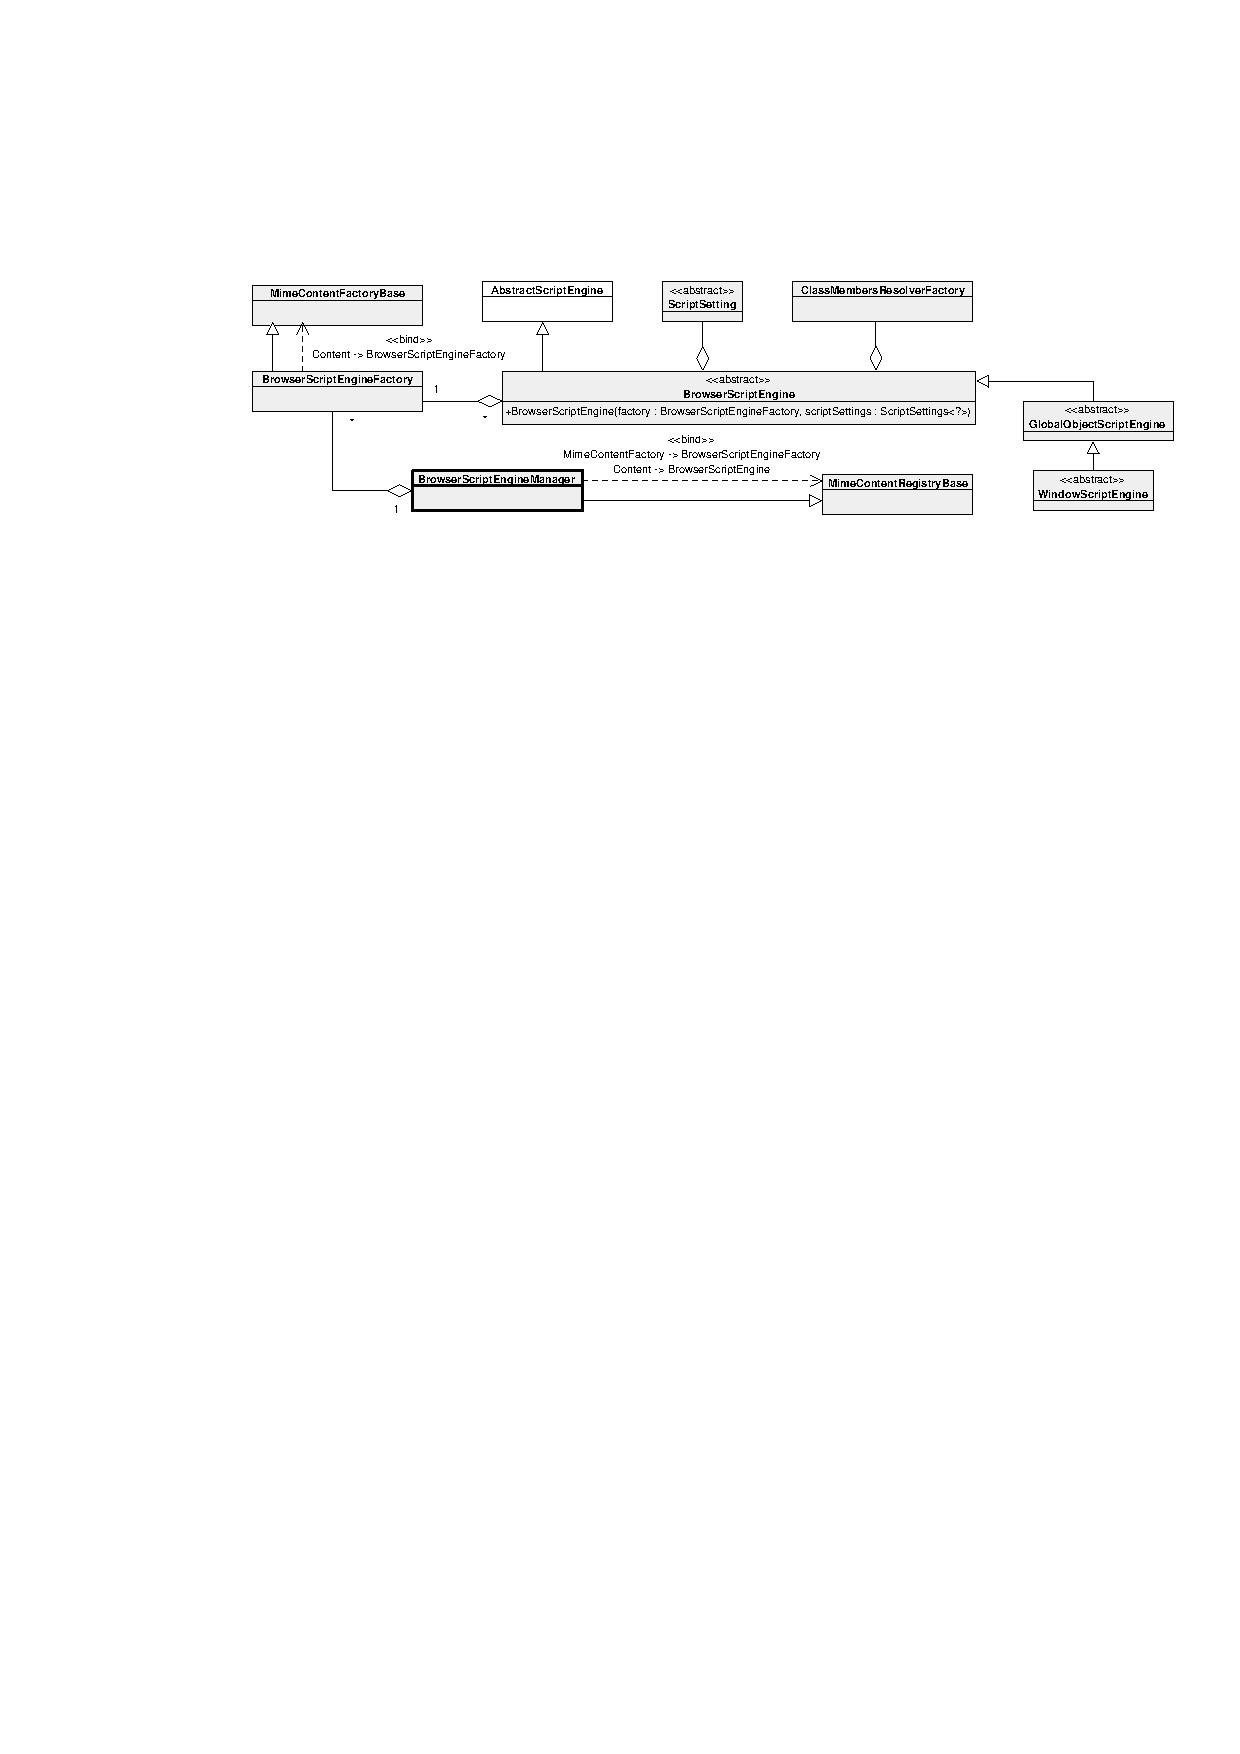
\includegraphics{fig/org-fit-cssbox-scriptbox-script-BrowserScriptEngine.pdf}
    }
    \caption{Diagram tříd znázorňující abstraktní skriptovací engine}
    \label{Figure.BrowserScriptEngine}
  \end{center}
\end{figure}

\vspace{-1em}

Všechny skriptovací enginy jsou vytvářeny pro některý konkrétní dokument, nad nímž je skriptovacím enginem uchováván skriptovací kontext. Pro jaký dokument byl skriptovací engine vytvořen, lze zjistit z nastavení pro skripty \texttt{ScriptSettings}, které je předáváno abstraktnímu skriptovacímu enginu během jeho konstrukce. V~rámci třídy abstraktního skriptovacího enginu se s objektem \texttt{ScriptSettings} přímo nepracuje, ale v~dalších specifičtějších třídách je dále využíván pro zjišťování globálního objektu. Globální objekt bývá obvykle konkrétními skriptovacími enginy implementován do enginového scopu daného skriptovacího enginu. Konkrétně třída \texttt{WindowScriptEngine} reprezentuje rozhraní pro zabudování globálního objektu \texttt{Window}.

Každý skriptovací engine \texttt{BrowserScriptEngine} obsahuje referenci na továrnu resolverů členů tříd \texttt{ClassMembersResolverFactory}. Resolver je použit k určení viditelných členů exportovaných objektů Javy pro implementaci globálního objektu a~blíže je popsán v~následující kapitole \ref{Chapter.Implementation.ExportConcepts}. 

Skriptovací enginy jsou vytvářeny továrnami \texttt{BrowserScriptEngineFactory}, které jsou evidovány a~registrovány v~singleton třídě \texttt{BrowserScriptEngineManager}. Manažerská třída všechny továrny skriptovacích enginů spravuje. Na dotázání třída továrny poskytuje vnějšímu okolí nebo případně ihned vytváří konkrétní skriptovací enginy některé továrny. Třídy \texttt{BrowserScriptEngineFactory} a~\texttt{BrowserScriptEngineManager} rozšiřují třídy pro spravování továren obsahů v~závislosti na MIME typu obsahu, které byly blíže popsány v~kapitole \ref{Chapter.Implementation.ContentHandling}. Rozhodujícím faktorem pro vybrání odpovídající továrny skriptovacího enginu je MIME typ skriptu, na jehož základě je v~manažeru továren vyhledáváno.

\subsection{Koncepty exportu objektů Javy}
\label{Chapter.Implementation.ExportConcepts}

Z důvodu snadného přidávání nové implementace klientských skriptovacích enginů byly implementovány koncepty exportu nativních objektů Javy do kontextů skriptovacích enginů. Když chceme exportovat objekt, je výhodné vědět a~určit, které prvky objektu mají být exportovány a~jak by tyto prvky měly být reprezentovány v~klientských skriptovacích enginech. Prvky zde myslíme členy třídy -- atributy, metody nebo konstruktory třídy. Za účelem specifikace exportovatelných členů tříd vznikla podpora, která přesně vyčleňuje jednotlivé členy tříd. Exportovatelné členy jsou vyhodnocovány ve třídách rozšiřující abstraktní třídu \texttt{ClassMembers}. Výchozí a~jediná implementace pro určování členů tříd je hotova ve třídě \texttt{DefaultClassMembers}. Abstraktní třída \texttt{ClassMembers} vlastní odkaz na třídu, jejíž členy jsou vyhodnocovány, a~odkaz na resolver, který jednotlivé členy rozpoznává. 

\begin{figure}[H]
  \begin{center}
    \scalebox{0.75}{
      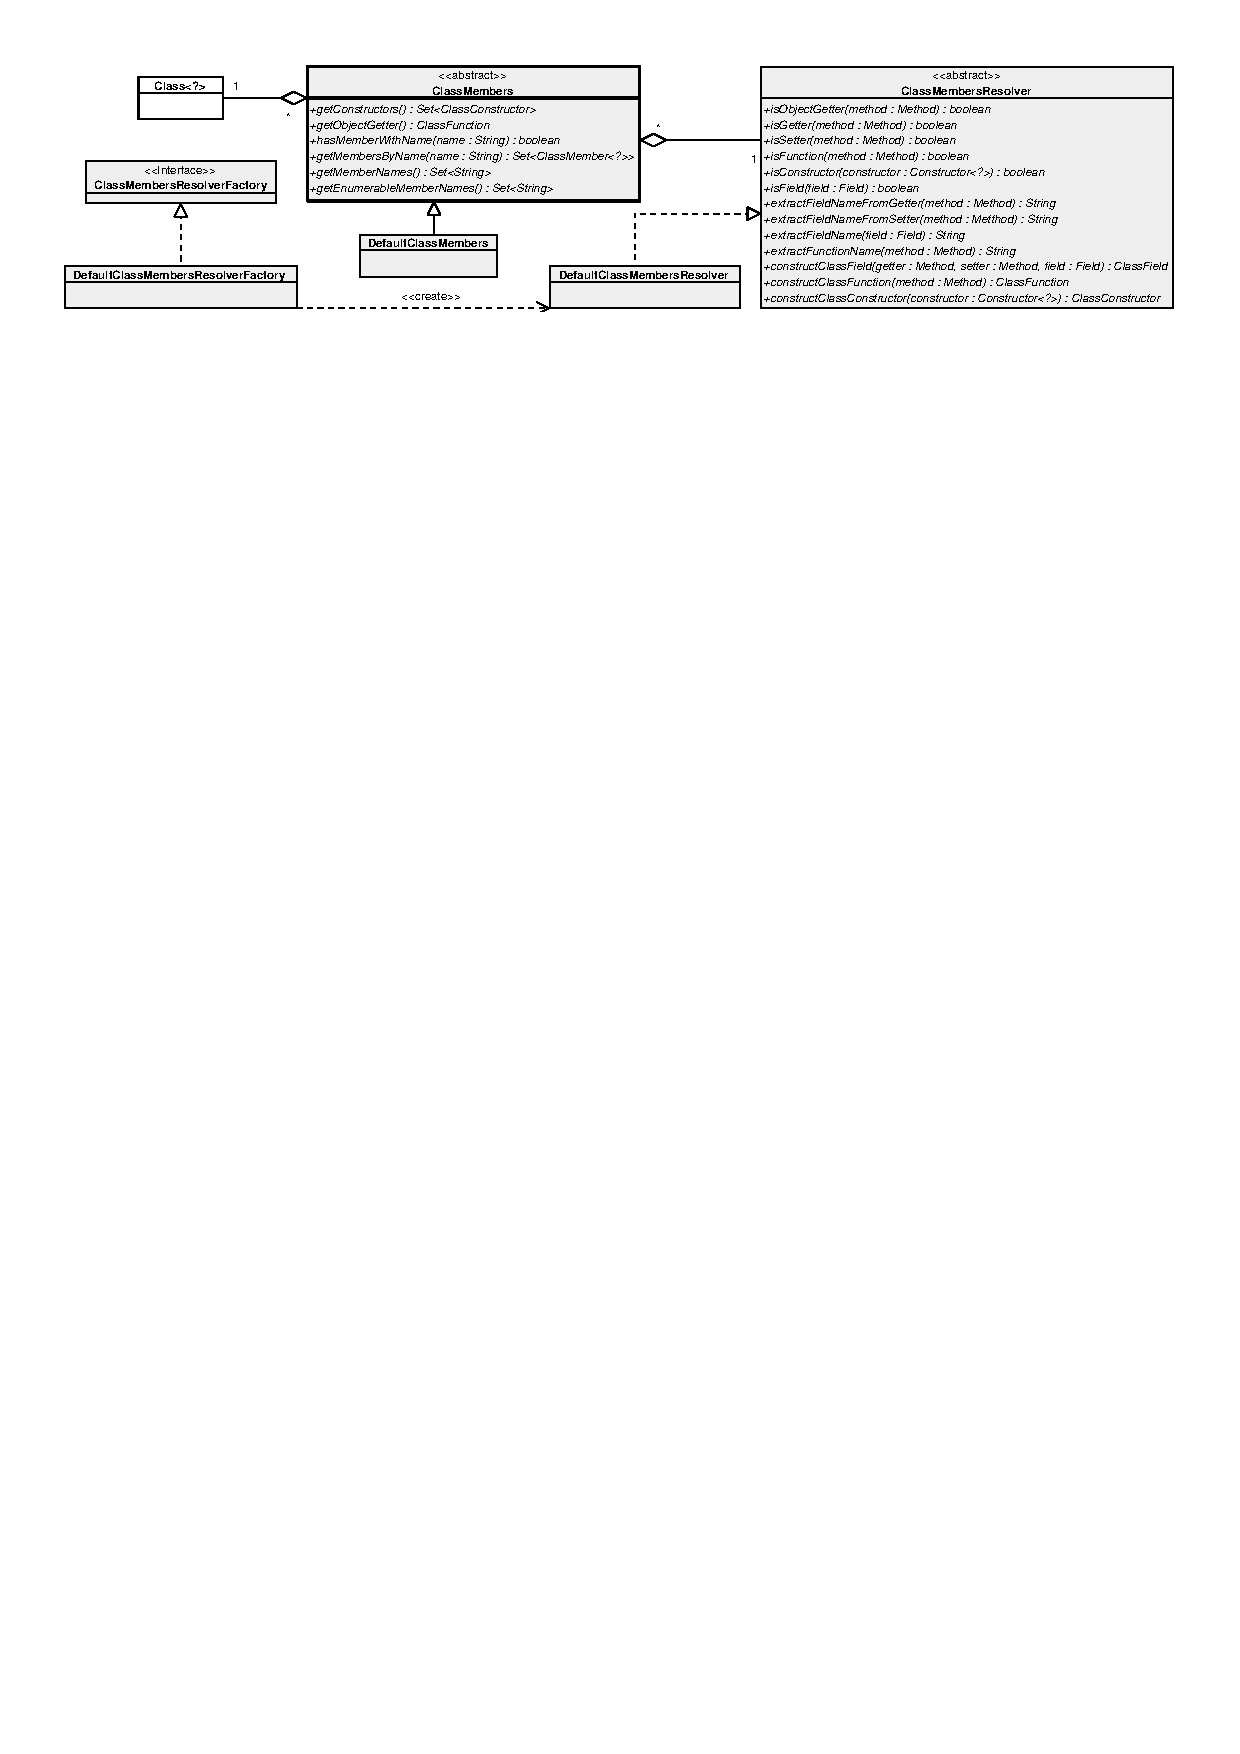
\includegraphics{fig/org-fit-cssbox-scriptbox-script-reflect-ClassMembers.pdf}
    }
    \caption{Diagram tříd znázorňující třídu reprezentující členy tříd}
    \label{Figure.ClassMembers}
  \end{center}
\end{figure}

\vspace{-1em}

Třídy resolverů slouží náležitou implementací metod začínajících prefixem \texttt{is\ldots()} k~určení, zda má být Java člen exportován nebo nikoliv. Pokud je člen exportovatelný, pak resolvery zprostředkovávají i extrakci názvů členů, pod kterými jsou členy viditelné v~klientských skriptech. Pro účel extrakce jsou vyčleněny metody začínající prefixem \texttt{extract\ldots()}. Závěrem resolvery vytváří metodami s prefixem \texttt{construct\ldots()} obaly exportovatelných standardních Java členů -- členů \texttt{Constructor}, \texttt{Field} a~\texttt{Method}. Poslední metodou poskytovanou resolvery, je metoda testu \texttt{isObjectGetter()} ověřující, zda je předaná metoda metodou pro indexované získávání objektů z objektu zkoumané třídy. Asociativní získávání objektů z objektu, neboli vytvoření asociativního pole z objektu, bylo implementováno z důvodu potřeby indexovaného získávání objektů \texttt{WindowProxy} vnořených procházecích kontextů z objektu \texttt{Window} podle jejich jména nebo indexu. Výchozí resolver \texttt{DefaultClassMembersResolver} exportuje všechny členy tříd Javy, přičemž jejich názvy extrahuje pomocí reflexe.

Pro rozšíření funkčnosti standardních Java členů byly vytvořeny speciální obalující třídy \texttt{ClassFunction}, \texttt{ClassConstructor} a~\texttt{ClassField} tak, jak je znázorněno na obrázku \ref{Figure.ClassMember}. Obaly Java členů přidávají metody pomocné metody pro export a~hlavně obsahují odkaz na pole možností \texttt{options}, které specifikuje způsob, jak by měl být člen implementován v~klientském skriptu. V~současné implementaci je možno uchovávat možnosti:

\begin{itemize}
  \item \textbf{\texttt{ENUMERABLE}} -- slouží pro určení, zda člen bude zúčastněn v~seznamu všech výčtových členů objektu. V~JavaScriptu umožňuje povolit nebo zabránit výpisu vlastnosti objektu, např. při průchodu \texttt{for (var property in object)}. Tato možnost reflektuje ECMAScript atribut \texttt{[[Enumerable]]}.
  \item \textbf{\texttt{PERNAMENT}} -- zda člen bude natrvalo svázán s objektem, v~němž je definován, nebo může být přepsán během vykonávání skriptu za uživatelský objekt. Tato možnost zjednodušeně reflektuje Web IDL atributy \texttt{[Unforgeable]} a~[Replaceable].
\end{itemize}

\begin{figure}[H]
  \begin{center}
    \scalebox{0.75}{
      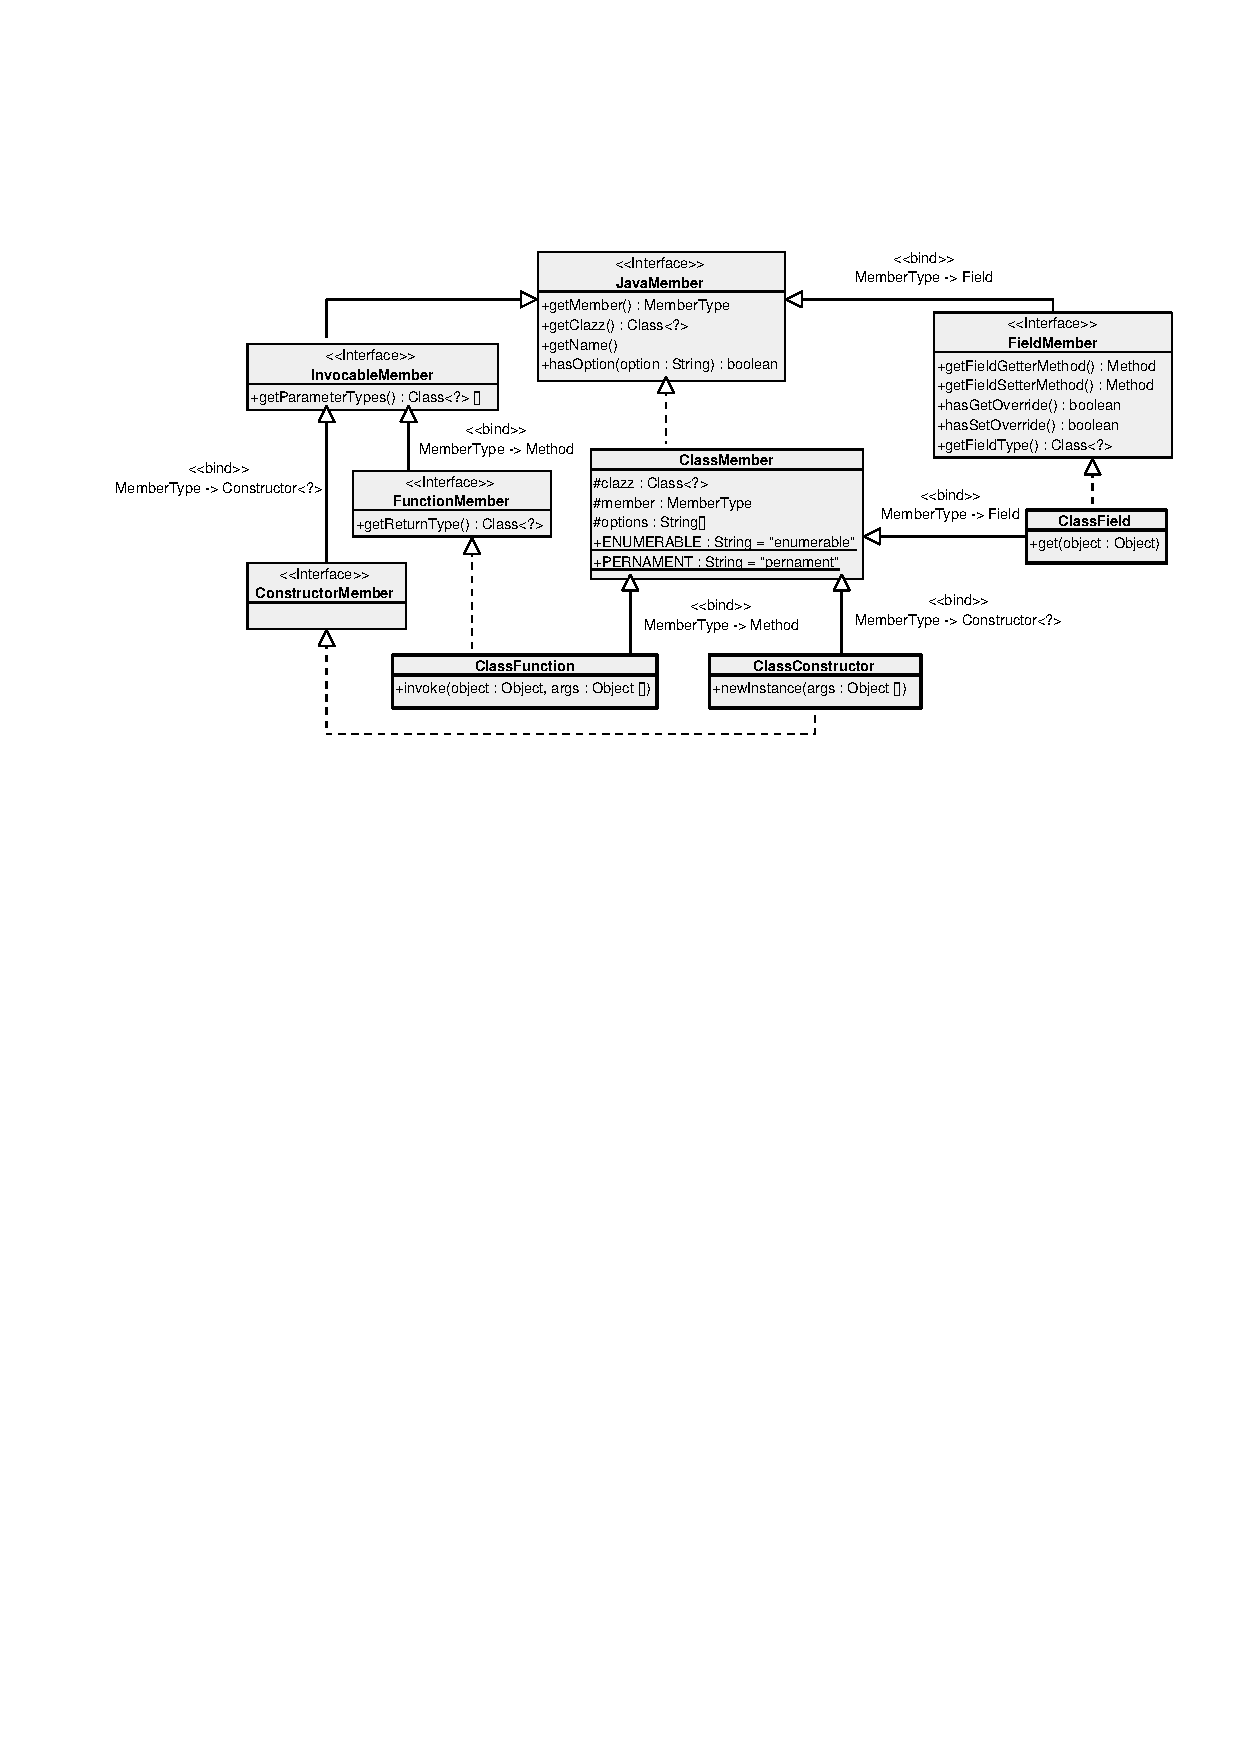
\includegraphics{fig/org-fit-cssbox-scriptbox-script-reflect-ClassMember.pdf}
    }
    \caption{Diagram tříd znázorňující třídy členů}
    \label{Figure.ClassMember}
  \end{center}
\end{figure}

\vspace{-1em}

Z důvodu uchovávání a~svázání členů tříd s objekty, které byly exportovány, byly implementovány třídy členů objektů: \texttt{ObjectFunction}, \texttt{ObjectConstructor}, \texttt{ObjectField}. Tyto třídy, jako třídy členů tříd, implementují rozhraní \texttt{FunctionMember}, \texttt{ConstructorMember} a~\texttt{FieldMember}. Strom dědičnosti tříd členů objektů je obdobný jako u členů tříd. Objekty členů navíc od objektů členů uchovávají instanci exportovaného objektu, ale implementačně se od tříd členů tříd příliš neliší, proto zde nebudou blíže popisovány.

\subsection{Export objektů založený na anotacích}
\label{Chapter.Implementation.AnnotationExportConcepts}

Systém exportu nativních objektů Javy využívající výchozí implementací resolveru členů třídy \texttt{DefaultClassMembersResolver}, popsaný v~předchozí kapitole \ref{Chapter.Implementation.ExportConcepts}, umožňoval kompletní export objektů do klientských skriptů. Kompletní export není ovšem téměř nikdy žádoucí, jelikož do exportu jsou zahrnuty i např. metody třídy \texttt{Object}, ze které dědí každá třída Javy. Velmi často se prolíná vnitřní implementace členů objektu pro export a~implementace členů, který by měly být ve skutečnosti exportovány. Nastala otázka, jak jednotlivé členy odlišit. Řešení se nabídlo v~anotacích Javy, díky kterým bylo možné přesně určit exportovatelné členy a~rozšířit exportování o další přídavné funkčnosti.

\begin{figure}[H]
  \begin{center}
    \scalebox{0.75}{
      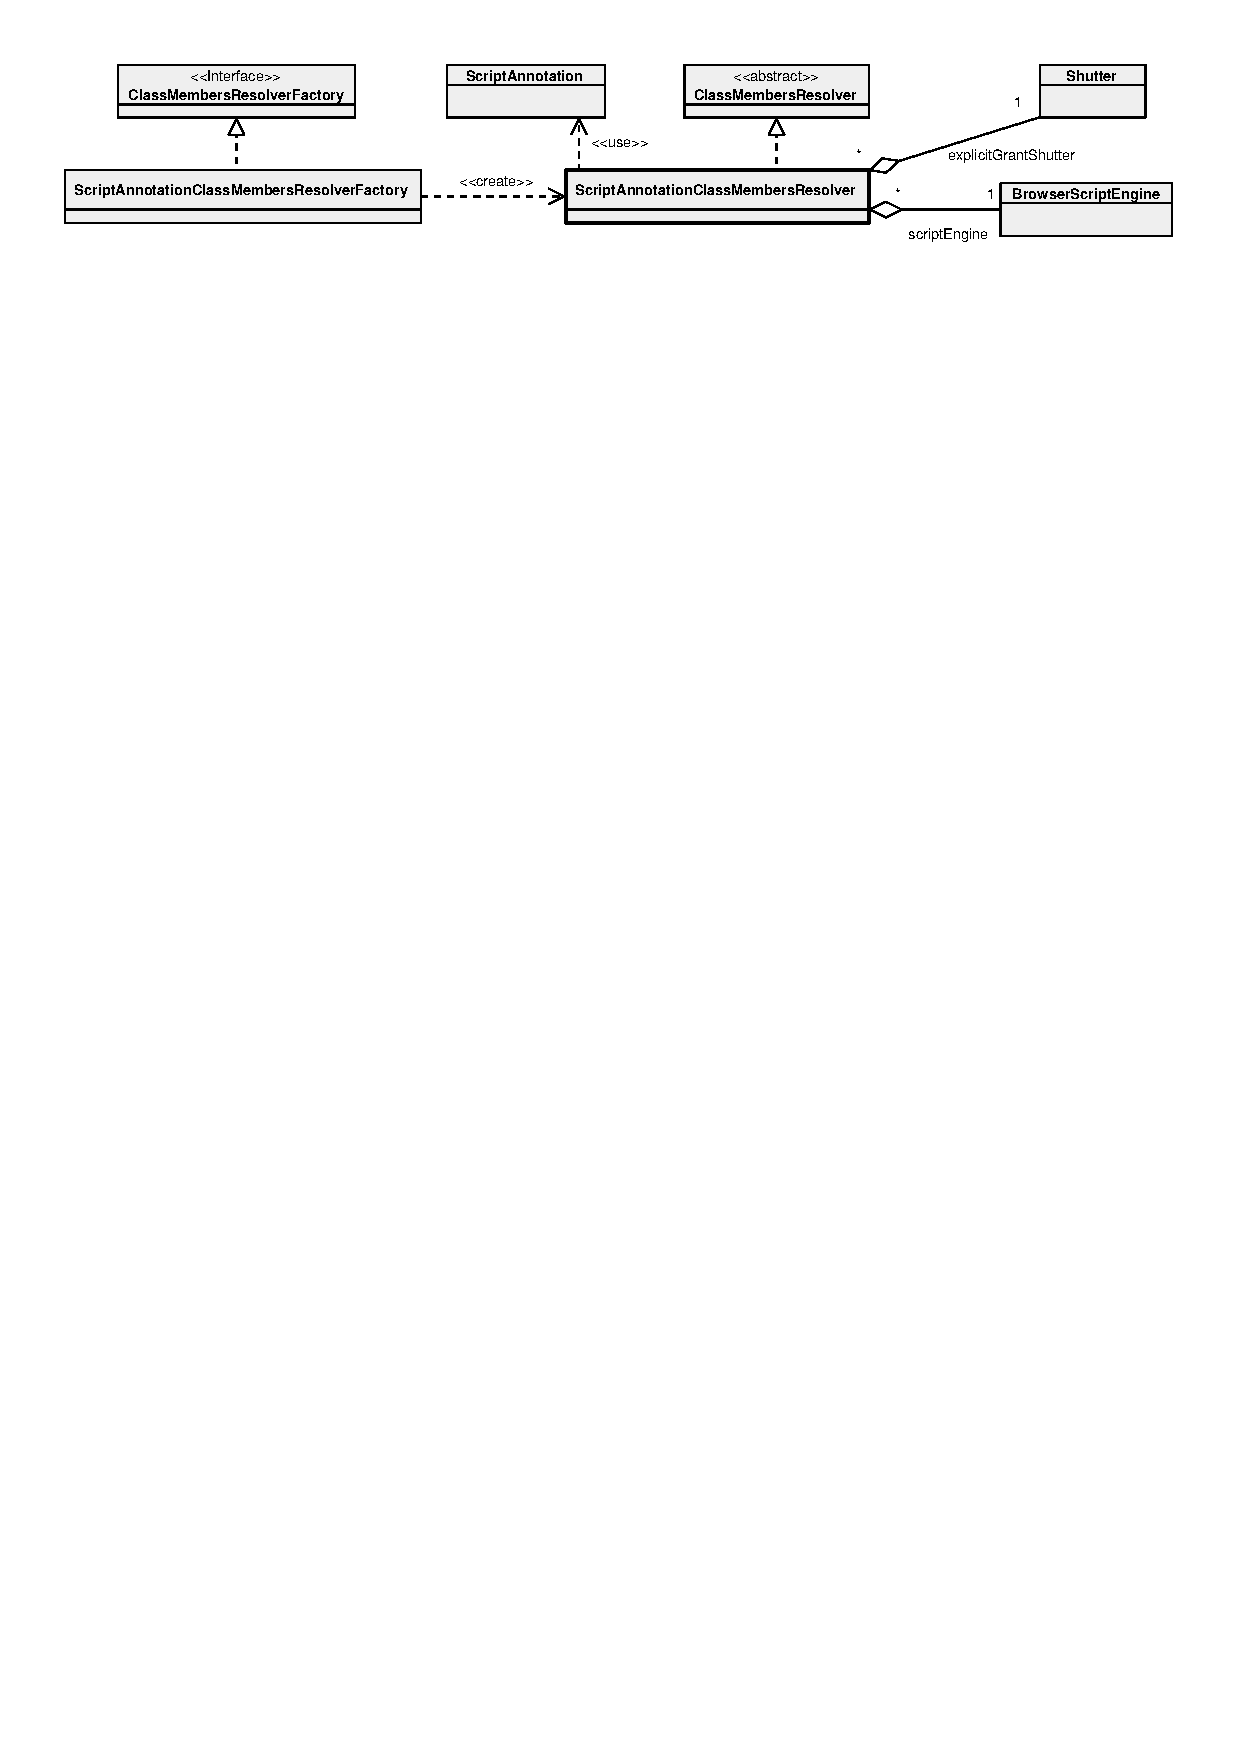
\includegraphics{fig/org-fit-cssbox-scriptbox-script-annotation-ScriptAnnotationClassMembersResolver.pdf}
    }
    \caption{Diagram tříd znázorňující resolver členů tříd založený na anotacích}
    \label{Figure.AnnotationClassMembersResolver}
  \end{center}
\end{figure}

\vspace{-1em}

Pro export založený na anotacích členů tříd byl vytvořen nový resolver členů implementovaný třídou \texttt{ScriptAnnotationClassMembersResolver}. Resolver pro svoji funkci potřebuje referenci na skriptovací engine, který provádí vyhodnocování členů tříd. Bez znalosti skriptovacího enginu bychom nemohli rozhodnout, zda je daný člen exportovatelný pro konkrétní skriptovací engine. Pokud by bylo žádoucí exportování stejných členů do všech skriptovacích enginů a~nemít možnost volby skriptovacího enginu, pro který je export validní, pak by reference na skriptovací engine nemusela existovat. Třída resolveru obsahuje ještě referenci na objekt \texttt{Shutter}, který zde neslouží k restrikci přístupu pro určité členy, třídy a~balíčky, nýbrž k explicitnímu povolování členů, které nenesou žádnou anotaci. Pro implementaci funkčnosti třídy resolveru se využívá pomocné třídy \texttt{ScriptAnnotation}, ve které se nachází pouze statické metody. Metody pomáhají určit, zda je daný člen exportovatelný na základě anotací pro daný skriptovací engine.

V~současné implementaci jsou podporovány skriptovací anotace pro členy třídy a~třídy uvedené v~ tabulce \ref{Table.SupportedEvents}.

\begin{table}[H]
  \begin{center} 
    \begin{tabular}{|l|c|p{6cm}|} \hline
    \theadStart{Anotace} & \thead{Působnost anotace} & \thead{Popis funkce anotace} \\ \hline
    \texttt{@InvisibleField} & Atribut & Zabránění exportu atributu \\ \hline
    \texttt{@InvisibleFunction} & Metoda & Zabránění exportu funkce\\ \hline
    \texttt{@ScriptClass} & Třída & Anotace pro exportovatelnou třídu -- nemusí být uvedena \\ \hline
    \texttt{@ScriptConstructor} & Konstruktor & Exportovatelný konstruktor objektu\\ \hline
    \texttt{@ScriptField} & Atribut & Exportovatelný atribut \\ \hline
    \texttt{@ScriptFunction} & Metoda & Exportovatelná funkce \\ \hline
    \texttt{@ScriptGetter} & Metoda & Exportovatelný atribut na základě getter metody \\ \hline
    \texttt{@ScriptSetter} & Metoda & Exportovatelný atribut na základě setter metody \\ \hline
    \end{tabular}
    \caption{Třídy podporovaných událostí}
    \label{Table.SupportedEvents}
  \end{center}
\end{table}

\vspace{-1em}

Každá skriptovací anotace obsahuje některé atributy, které omezují a~ovlivňují export členů tříd. Všechny anotace mají společný jeden atribut \texttt{engines} s polem skriptovacích enginů, pro které je daná anotace validní. Pokud je pole \texttt{engines} prázdné, pak se předpokládá, že je člen s touto anotací viditelný pro všechny skriptovací enginy. 

Jedinou anotací, která není určena pro členy třídy, je anotace \texttt{@ScriptClass}, jež se uvádí nad typem třídy. Tato anotace umožňuje definovat rozsah automatického zahrnutí exportovatelných členů třídy, bez nutnosti definování odpovídající anotace u daného členu. Anotace přidává k popsanému atributu \texttt{engines} další atribut s polem \texttt{options}. Pokud zahrneme v~poli s možnostmi anotace \texttt{options}, např. hodnotu \texttt{ALL\_METHODS}, tak budou exportovány všechny metody dané třídy, nad kterou je anotace uvedena. Další podporované možnosti anotace jsou: \texttt{ALL\_FIELDS}, \texttt{ALL\_STATIC\_METHODS}, \texttt{ALL\_STATIC\_FIELDS}, \texttt{ALL\_CONSTRUCTORS}. Jedinými anotacemi, které mohou ovlivnit automatické exporty po uvedení některé možnosti anotace \texttt{@ScriptClass}, jsou anotace exkluze \texttt{@InvisibleField} a~\texttt{@InvisibleFunction}. Tyto anotace slouží k zabránění exportu členu třídy, který by byl normálně exportován. 

Když žádáme vytvoření některého atributu v~klientském skriptu, máme hned tři možnosti jak toho docílit. Pro definici atributu můžeme použít anotaci \texttt{@ScriptField}, která přímo zpřístupní atribut, nad kterým je anotace uvedena. Dále máme k dispozici anotace \texttt{@ScriptGetter} a~\texttt{@ScriptSetter}, které vytvoří atribut z getter nebo setter metody, nad níž je anotace uvedena. Resolver pro anotace umožnuje pro všechny tři uvedené anotace automatické odvození názvu atributu. Název~atributu lze předefinovat uvedením atributu anotace \texttt{field}, kde lze zvolit vlastní název~pro atribut pro klientské skriptovací enginy. Pokud je jeden a~tentýž atribut definován na více místech pomocí různých anotací, pak lze zvolit, zda by mělo mít přednost volání getteru nebo setter pro získávání atributu před přímým přístupem k atributu. Přednosti getterů a~setterů se definují v~možnostech anotací hodnotou \texttt{FIELD\_GET\_OVERRIDE} nebo \texttt{FIELD\_SET\_OVERRIDE}. Chceme-li zahrnout metody getterů a~setterů do exportovatelných funkcí, pak lze v~možnostech anotace uvést hodnotu \texttt{CALLABLE\_GETTER} nebo \texttt{CALLABLE\_SETTER}.

U všech výše uvedených anotací, které sloužily pro export členu třídy, lze také zvolit, zda by tento člen měl mít nastavenou vlastnost \texttt{ENUMERABLE} popsanou v~kapitole \ref{Chapter.Implementation.ExportConcepts}. Vlastnost \texttt{PERNAMENT} nelze v~současné implementaci nastavovat. Proto všechny členy exportované pomocí skriptovacích anotací mají pevně nastavenou vlastností \texttt{PERNAMENT}.

\subsection{Další implementovaná funkčnost}
\label{Chapter.Implementation.OtherFunctionality}

V~kapitole \ref{Chapter.Design.GlobalScopeInjections} jsme navrhli injekci do hlavního scopu. Koncept injekce byl kompletně dodržen tak, jak byl navržen. Jednotlivé injektory \texttt{ScriptContextInjector} po zavolání metody \texttt{registerScriptContextInject()} registrují automaticky nesoucí injekci u všech továren skriptovacích enginů, ke kterým injektory náleží. Přejeme-li si zaregistrovat injektor u všech zaregistrovaných továren skriptovacích enginů, tak stačí během konstrukce injektoru předat speciální konstantu \texttt{ALL\_SCRIPT\_ENGINE\_FACTORIES}. V~současnosti jediným implementovaným injektorem, který je společný pro všechny skriptovací enginy uživatelského agenta, je \texttt{URLInjector}, který vkládá objekt pro konstrukci URL do hlavního scopu všech skriptovacích enginů. Pro JavaScriptový stroj byl dále implementován injektor vkládající speciální objekty, které reprezentují třídy klientského JavaScriptu, viz kapitola \ref{Chapter.Implementation.GlobalScopeImplementation}. Posledním implementovaným injektorem je injektor vkládající objekt konzole v~rámci ukázkové aplikace. 

Během implementace se vyskytla potřeba převádět objekty na různá rozhraní, nejčastěji rozhraní neobsahující skriptovací anotace na objekty, které jsou již anotované a~tak přístupné pro klientské skripty. Pro tento účel byl implementován jednoduchý registr adaptérů umožňující požadovanou funkčnost (obrázek \ref{Figure.AdapterRegistry}). Adaptéry jsou používány třeba pro převod Xerces implementace událostí \texttt{EventImpl}, \texttt{MouseEventImpl} na třídy \texttt{AdaptedEvent}, \texttt{AdaptedMouseEvent} za pomocí adapterů \texttt{EventAdapter} a~\texttt{MouseEventAdapter}. Jednotlivé skriptovací enginy by měly využívat tento registr adaptérů při zviditelňování nativních objektů Javy v~klientských skriptech.

\begin{figure}[H]
  \begin{center}
    \scalebox{0.50}{
      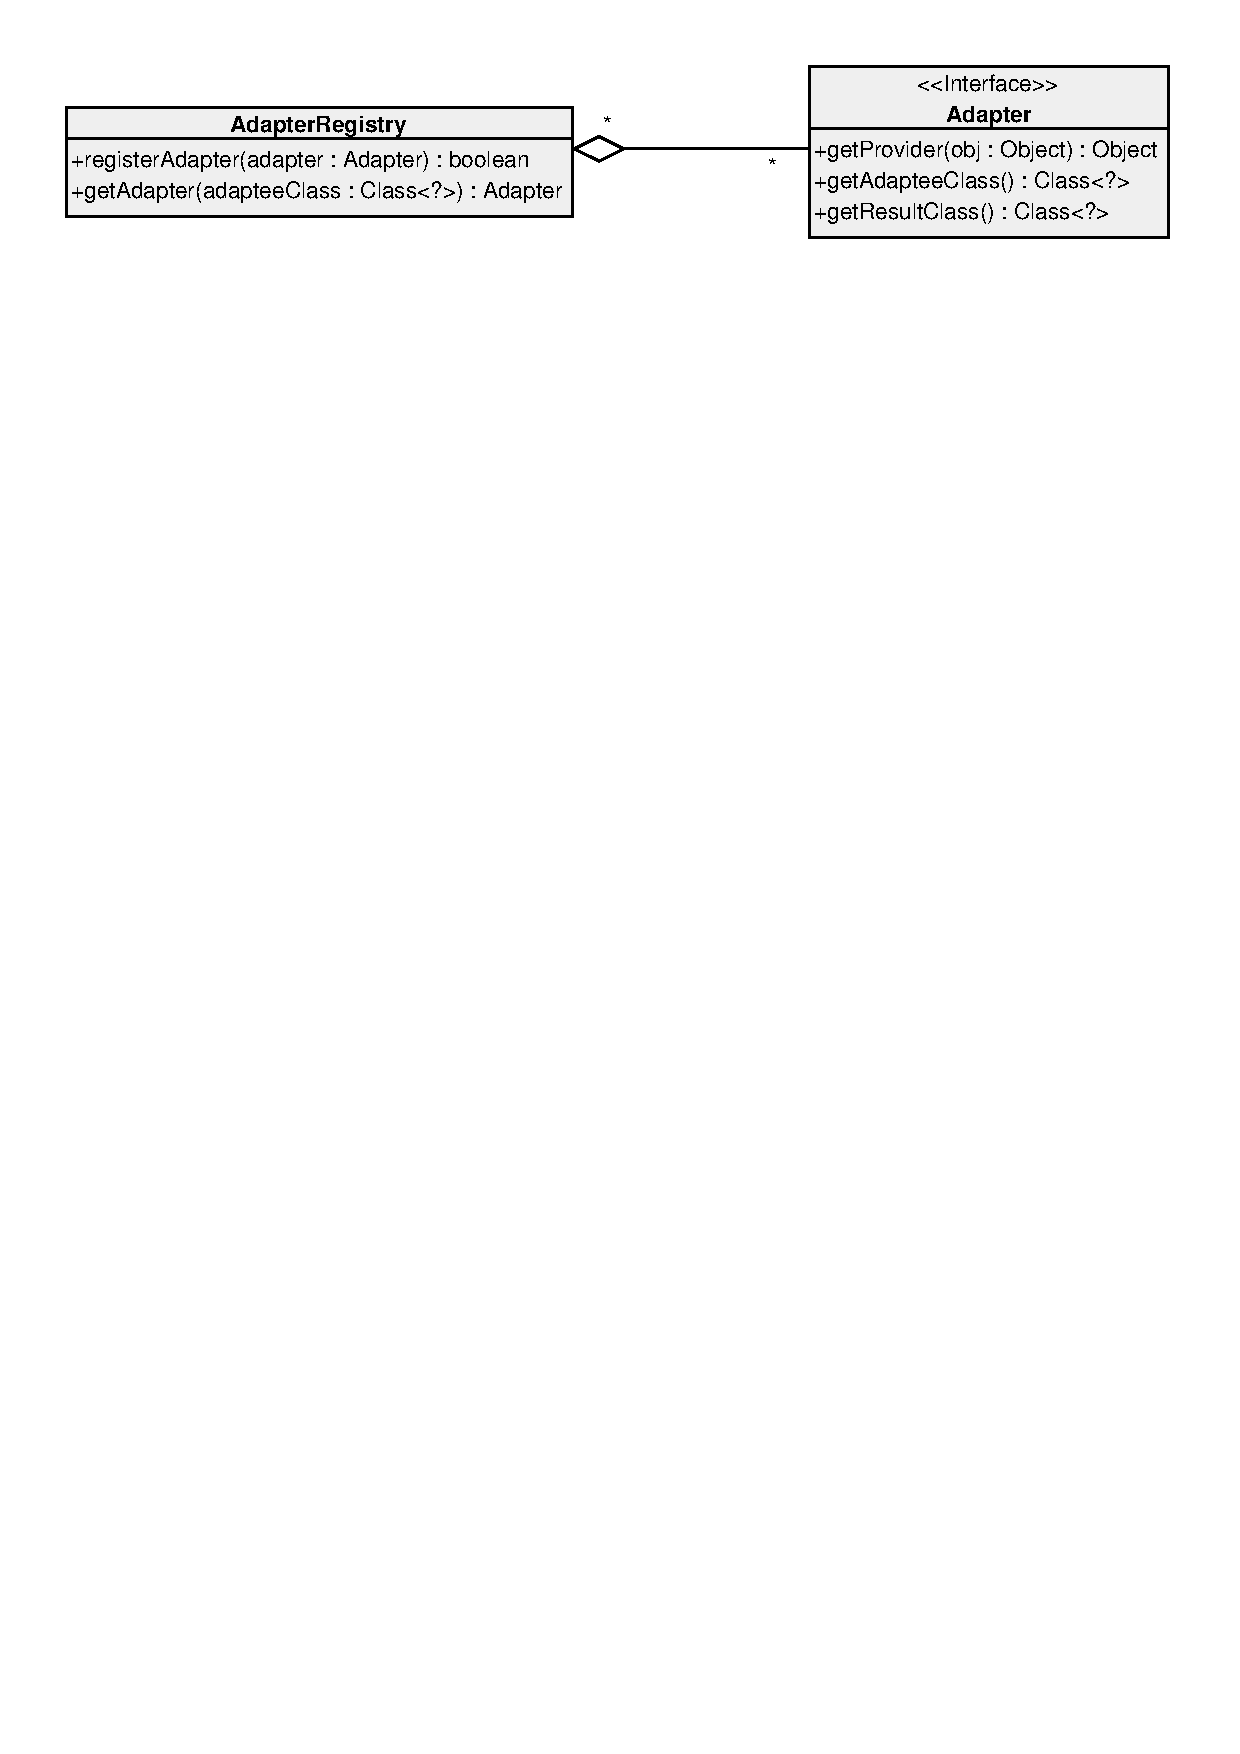
\includegraphics{fig/org-fit-cssbox-scriptbox-script-adapter-Adapter.pdf}
    }
    \caption{Diagram tříd znázorňující registr adaptérů}
    \label{Figure.AdapterRegistry}
  \end{center}
\end{figure}

\vspace{-1em}

\section{Klientský JavaScriptový engine}
\label{Chapter.Implementation.JavaScriptEngine}

V~minulých kapitolách jsme popsali obecné společné rozhraní pro všechny skriptovací enginy. V~této kapitole se zaměříme na konkrétní implementaci jediného skriptovacího enginu, který je nyní podporován -- skriptovacího enginu JavaScriptu.

JavaScriptový skriptovací engine byl implementován s využitím knihovny Rhino, která poskytuje jádro interpretu JavaScriptu. Implementovaný skriptovací engine je kompatibilní se specifikací JSR 223. Implementace JavaScriptového enginu podle JSR 223 v~JDK nebylo využito z důvodu přizpůsobení skriptovacího enginu a~kompletní kontroly nad zabudovaným prostředím Rhino. Standardní skriptovací API pro engine bylo implementováno zcela od základu. Jakým způsobem proběhlo propojením s Rhinem, je uvedeno v~kapitole \ref{Chapter.Implementation.JavaScriptEngineInterface}.

V~rámci konstrukce skriptovacího enginu dochází k tvorbě globálního scopu. Proces, který implementuje atributy a~metody globálního objektu do globálního scopu, je popsán v~kapitole \ref{Chapter.Implementation.GlobalScopeImplementation}. 

Knihovna Rhino exportuje nativní objekty Javy do prostředí JavaScriptu tak, že je zapouzdřuje do objektů NativeJavaObject, které implementují rozhraní \texttt{Scriptable}. Pro specifikaci členů objektů, které mají být implementovány, využívá Rhino třídy \texttt{JavaMembers}, která ovšem není veřejně přístupná. Z důvodu potřeby definice vlastních exportovatelných členů v~rámci exportovaných objektů Javy, bylo nutné vytvořit vlastní zapouzdřující objekt. Jak zapouzdření proběhlo, je popsáno v~kapitole \ref{Chapter.Implementation.NativeJavaWrappers}.

\subsection{Rozhraní JavaScriptového enginu}
\label{Chapter.Implementation.JavaScriptEngineInterface}

Skriptovací engine JavaScriptu je vytvářen továrnou \texttt{WindowJavaScriptEngineFactory}. V~implementaci jej představuje třída \texttt{WindowJavaScriptEngine} (obrázek \ref{Figure.WindowJavaScriptEngine}). Pro jedno vlákno může být vytvořen pouze jeden skriptovací engine. Omezení je dáno z důvodu, že je skriptovací engine přímo spjat s kontextem Rhina, který se vytváří pro aktuální běžící vlákno. Skriptovací kontext Rhina slouží pro běh skriptů a~je vytvářen před spuštěním nového skriptu. K vytváření kontextu se využívá továrny \texttt{JavaScriptContextFactory}, která je instanciována v~rámci konstrukce skriptovacího enginu. Během konstrukce enginu také dochází k vytvoření globálního scopu \texttt{TopLevel}, jehož tvorba je blíže popsána v~další kapitole \ref{Chapter.Implementation.GlobalScopeImplementation}.

\begin{figure}[H]
  \begin{center}
    \scalebox{0.75}{
      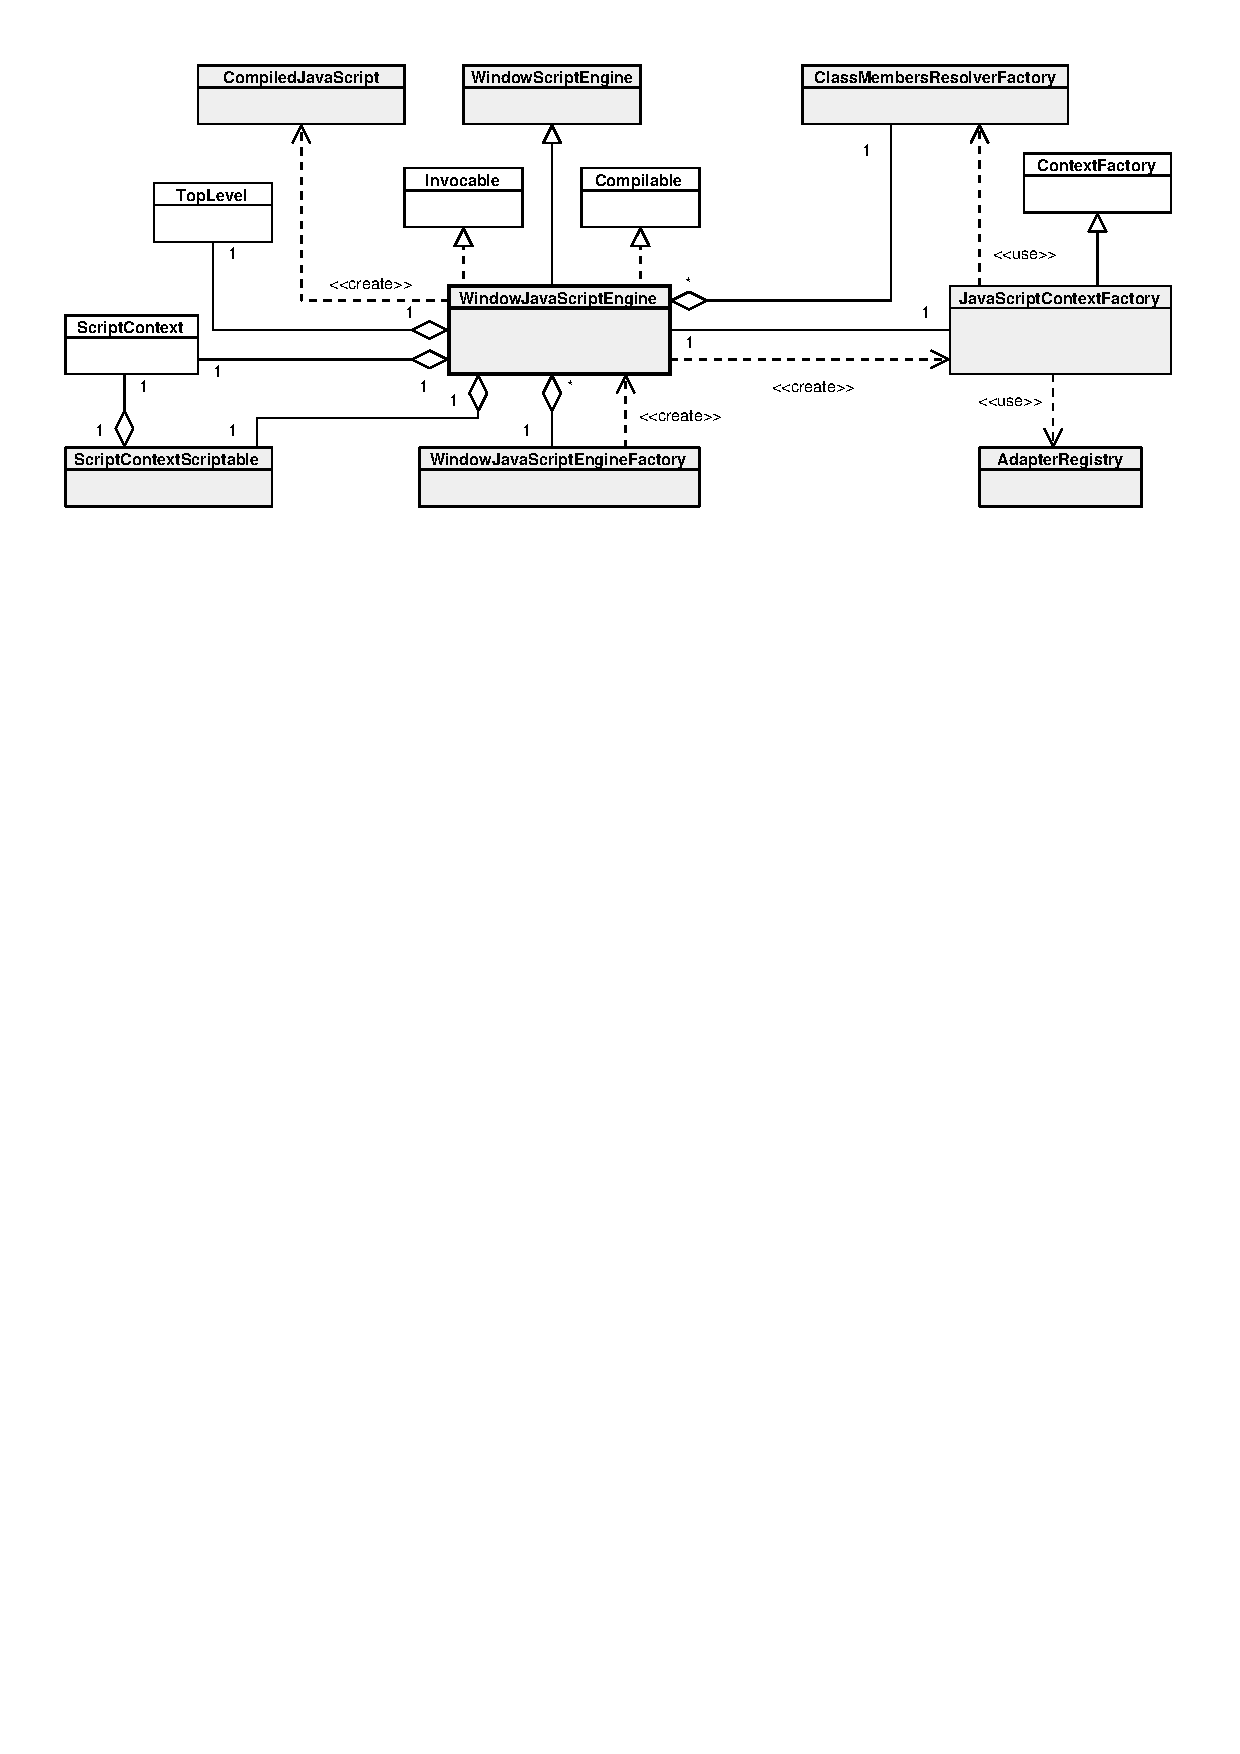
\includegraphics{fig/org-fit-cssbox-scriptbox-script-javascript-WindowJavaScriptEngine.pdf}
    }
    \caption{Diagram tříd znázorňující skriptovací engine JavaScriptu}
    \label{Figure.WindowJavaScriptEngine}
  \end{center}
\end{figure}

\vspace{-1em}

V~rámci konstrukce továrny skriptovacího kontextu \texttt{JavaScriptContextFactory} se registrují jednotlivé podporované adaptéry pro skriptovací engine. Aktuálně jsou registrovány adaptéry: \texttt{EventAdapter}, \texttt{UIEventAdapter}, \texttt{MouseEventAdapter} a~\texttt{ErrorAdapter}, jež převádí nativní objekty událostí na objekty viditelné ve skriptu. Když dochází k tvorbě kontextu, je pro kontext nastavena obalující továrna, která řetězí více metod obalování s využitím dekorátoru \texttt{WrapFactoryDecorator} blíže popsaného v~kapitole \ref{Chapter.Implementation.NativeJavaWrappers}.

Skriptovací engine vlastní referenci na továrnu resolverů členů tříd, která se využívá pro export nativních objektů Javy. V~aktuální implementaci se využívá továrny založené na anotacích \texttt{ScriptAnnotationClassMembersResolverFactory}. Skriptovací engine umožňuje volat funkce pomocí rozhraní \texttt{Invocable} nebo kompilovat skripty s využitím rozhraní \texttt{Compilable} do objektů \texttt{CompiledJavaScript}.

Abychom mohli implementovat data binding podle specifikace JSR 223, bylo nutno vytvořit speciální scope -- objekt \texttt{ScripContextScriptable}. Tento scope zpřístupňuje uložená data pomocí \texttt{Bindings} klientskému JavaScriptu a~naopak z klientského JavaScriptu zprostředkovává rozhraní pro uložení dat skriptu.

\subsection{Implementace globálního scopu}
\label{Chapter.Implementation.GlobalScopeImplementation}

V~rámci konstrukce skriptovacího enginu dochází k tvorbě globálního scopu. Globální scope je reprezentován v~Rhinu třídou \texttt{TopLevel}. Jelikož klientský JavaScript obsahuje globální scope, kde je implementován objekt \texttt{Window}, byla vytvořena rozšiřující třída \texttt{ObjectTopLevel} (obrázek \ref{Figure.ObjectTopLevel}), která daný objekt do globálního scopu vkládá. Globální objekt \texttt{Window} je získáván skriptovacím enginem z nastavení skriptu \texttt{ScriptSettings} a~dále předáván v~rámci konstrukce třídě \texttt{ObjectTopLevel}.

\medskip

\begin{figure}[H]
  \begin{center}
    \scalebox{0.75}{
      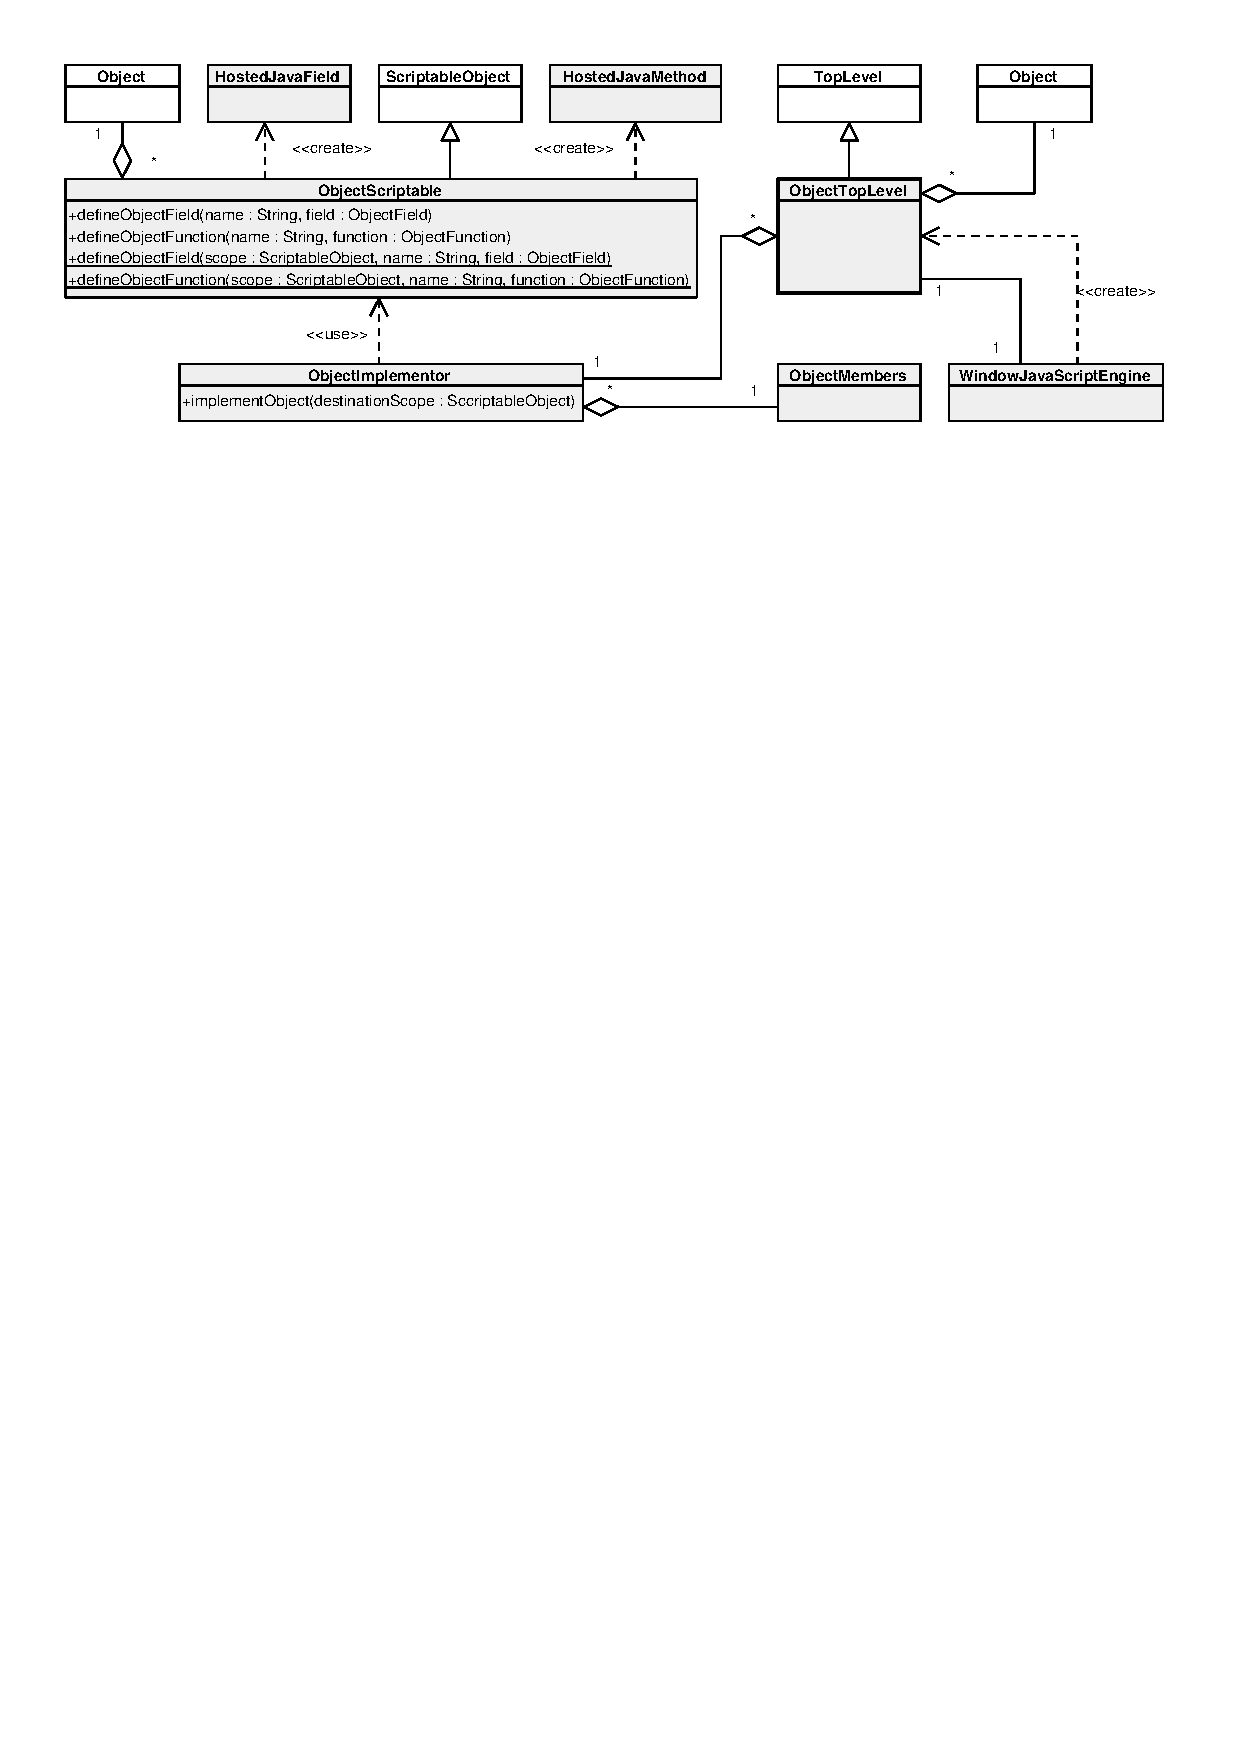
\includegraphics{fig/org-fit-cssbox-scriptbox-script-javascript-java-ObjectTopLevel.pdf}
    }
    \caption{Diagram tříd znázorňující objekt globálního scopu}
    \label{Figure.ObjectTopLevel}
  \end{center}
\end{figure}

Pro implementaci objektu do scopu využívá třída \texttt{ObjectTopLevel} instance implementátoru \texttt{ObjectImplementor}. Implementátor přijímá objekt, jenž má být implementován a~členy třídy implementovaného objektu získané ze skriptovacího enginu. Implementátor tak ve skutečnosti zná všechny členy objektu \texttt{ObjectMembers}, které by měly být v~globálním scopu implementovány. Členy objektu jsou implementovány s využitím veřejných statických metod třídy \texttt{ObjectScriptable}: \texttt{defineObjectField()} a~\texttt{defineObjectFunction()}. Třída \texttt{ObjectScriptable} je nadstavbou nad \texttt{ScriptableObject}, která umožňuje v~rámci své instance uchovat nativní objekt Javy, jenž sama tímto zapouzdřuje. Při zavolání metody \texttt{defineObjectField()} vytváří třída objekt \texttt{HostedJavaField}, který následně do předaného scopu vkládá. Po zavolání metody \texttt{defineObjectFunction()} vytváří třída nový objekt \texttt{HostedJavaMethod}, který taktéž vkládá do předaného scopu. Nachází-li se v~předaném scopu již jiný existující objekt \texttt{HostedJavaMethod}, pak je metoda \texttt{ObjectFunction} přidána do listu přetížených metod existujícího objektu \texttt{HostedJavaMethod}.

Globální scope implementuje standardní objekty Javy a~odstraňuje veškeré rozšiřující objekty Rhina, které by mohly narušit bezpečnost provádění skriptu, např. \texttt{JavaImporter}, \texttt{Packages}, \texttt{importClass}, \texttt{importPackage}, atd.

Z důvodu umožnění správné funkce operátoru instanceof, nebylo nutno do globálního scopu implementovat pouze globální objekt \texttt{Window}, ale také všechny objekty tříd. Přidání této podpory zajistil injektor \texttt{ClassObjectInjector} (obrázek \ref{Figure.ClassObjectsInjector}), který všechny třídy, jež by měly být viditelné ve skriptu, převádí na objekty \texttt{ClassScriptable}. Objekty \texttt{ClassScriptable} zapouzdřují objekt třídy a~předefinovávají metodu \texttt{hasInstance()}, která se volá při kontrole, zda je předaná instance typu, jenž zapouzdřuje objekt \texttt{ClassScriptable}.

\begin{figure}[H]
  \begin{center}
    \scalebox{0.53}{
      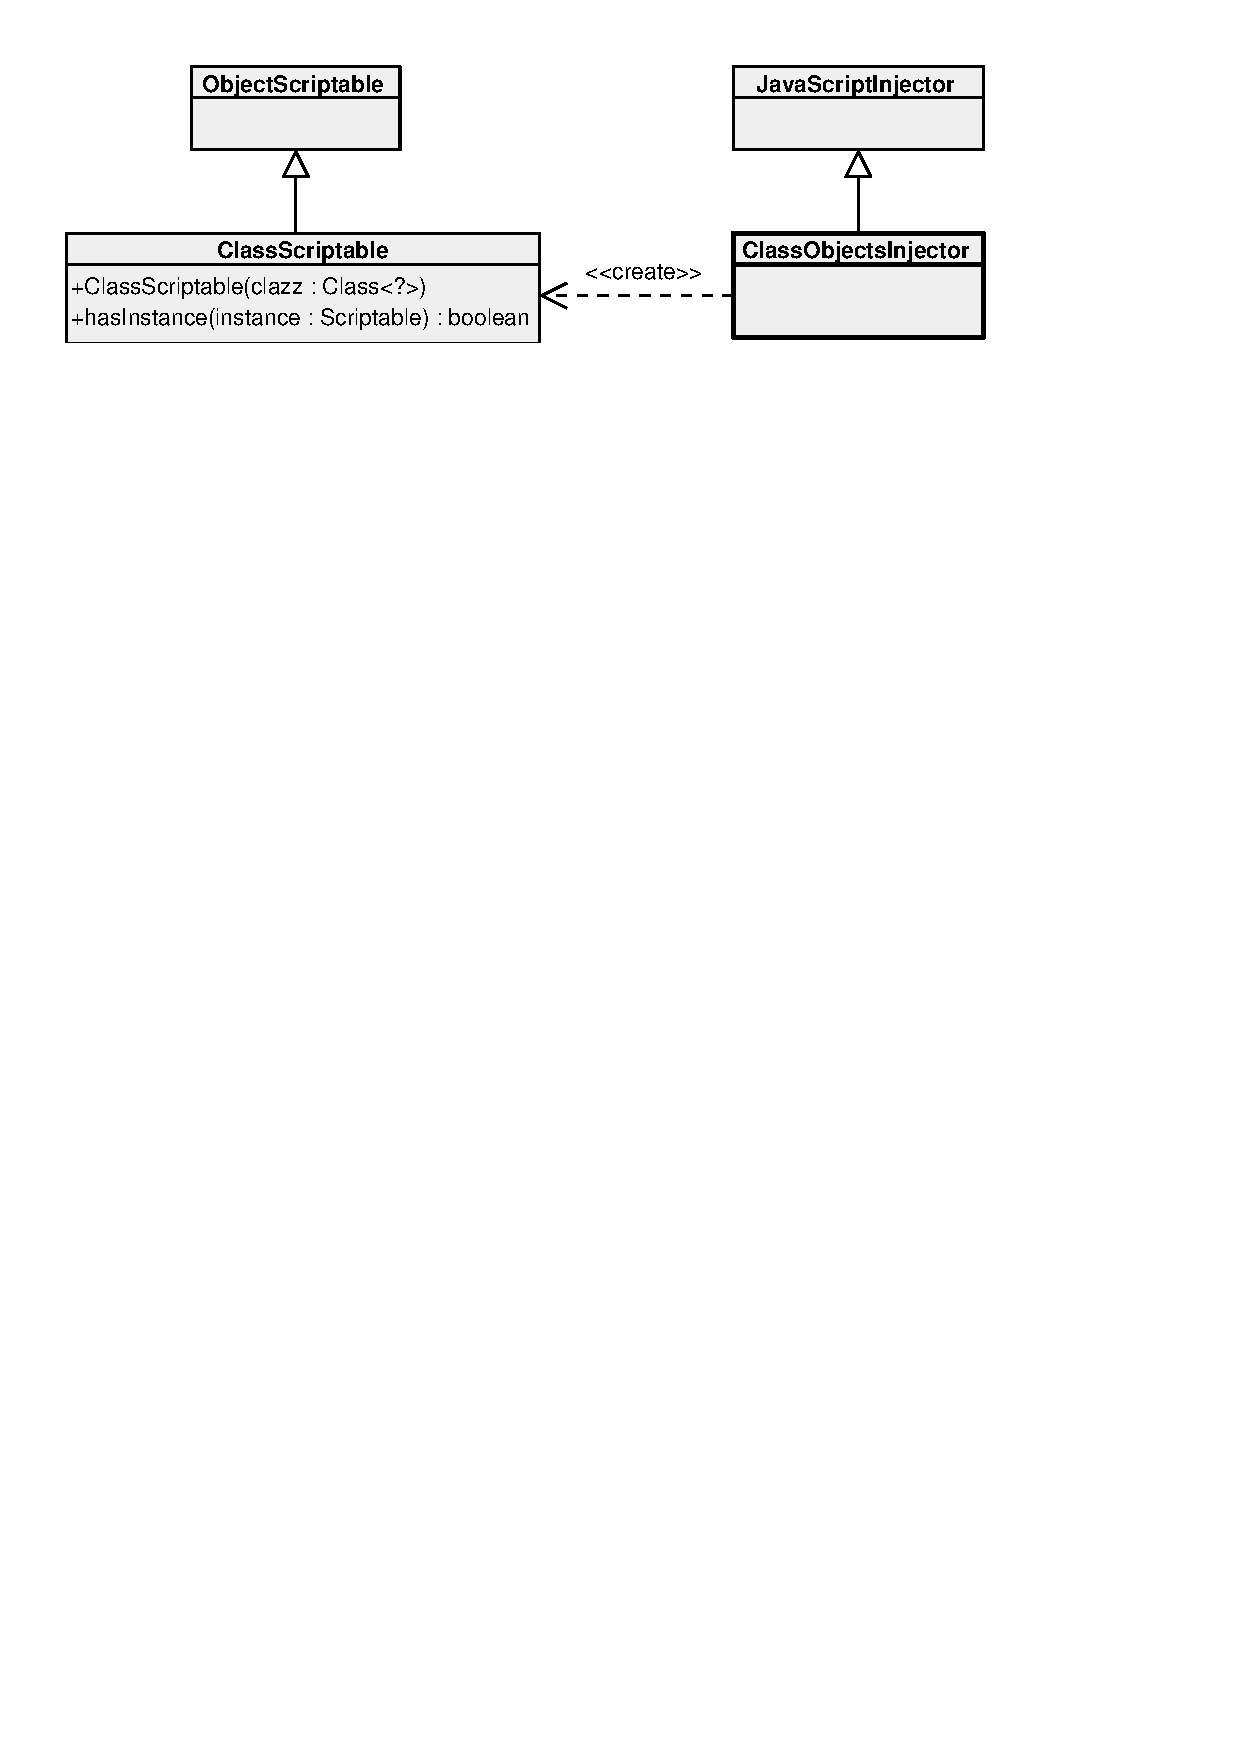
\includegraphics{fig/org-fit-cssbox-scriptbox-script-javascript-injectors-ClassObjectsInjector.pdf}
    }
    \caption{Diagram tříd znázorňující injektor globálního scopu}
    \label{Figure.ClassObjectsInjector}
  \end{center}
\end{figure}

\vspace{-3em}

\subsection{Zapouzdření nativních objektů Javy}
\label{Chapter.Implementation.NativeJavaWrappers}

Implementováním globálního scopu jsme získali množinu atributů a~metod, které mohou navracet nativní objekty Javy uživatelskému skriptu. Skriptovací engine ovšem nativním objektům Javy „nerozumí“ a~nedokáže s nimi pracovat, protože neimplementují rozhraní \texttt{Scriptable}. Knihovna Rhino řeší zapouzdřování objektů pomocí výchozí obalovací továrny \texttt{WrapFactory}, jejíž instance je uchovávána v~objekt kontextu Rhina. Implementace obalovací továrny zapouzdřuje nativní objekty do objektu \texttt{NativeJavaObject}.

Jelikož nebylo možné ovlivnit exportovatelné členy nativních objektů, bylo nutné vytvořit novou obalující továrnu, která vytváří nový obal pro nativní objekty reprezentovaný třídou \texttt{HostedJavaObject} (obrázek \ref{Figure.HostedJavaObject}). Obal nativního objektu \texttt{HostedJavaObject} zapouzdřuje nativní objekt, k němuž lze přistoupit např. rozbalením díky rozhraní \texttt{Wrapper}. Na rozdíl od globálního kontextu, obal neimplementuje všechny exportovatelné členy do scopu, nýbrž vytváří pouze rozhraní pro přímý přístup do zapouzdřených nativních objektů. Obal obsahuje referenci na všechny exportovatelné členy \texttt{ObjectMemers} zapouzdřeného objektu a~této reference využívá při potřebě získat nebo nastavit některou vlastnost zapouzdřeného objektu. Vlastnostmi zde máme na mysli i funkce zapouzdřeného objektu \texttt{ObjectFunction}, které předtím než je vrátíme z rozhraní \texttt{Scriptable}, musí být obaleny do nového objektu \texttt{HostedJavaMethod}. Kromě zajištění rozhraní \texttt{Scriptable} rozšířením třídy \texttt{ObjectScriptable}, obal \texttt{HostedJavaObject} implementuje také rozhraní \texttt{Function}. Rozhraní \texttt{Function} je implementováno za účelem umožnění volání exportovatelných konstruktorů zapouzdřeného objektu. Při volání operátoru \texttt{new} dochází k~zavolání metody \texttt{construct()}, které je obsaženo právě v~rozhraní \texttt{Function}.

\begin{figure}[H]
  \begin{center}
    \scalebox{0.60}{
      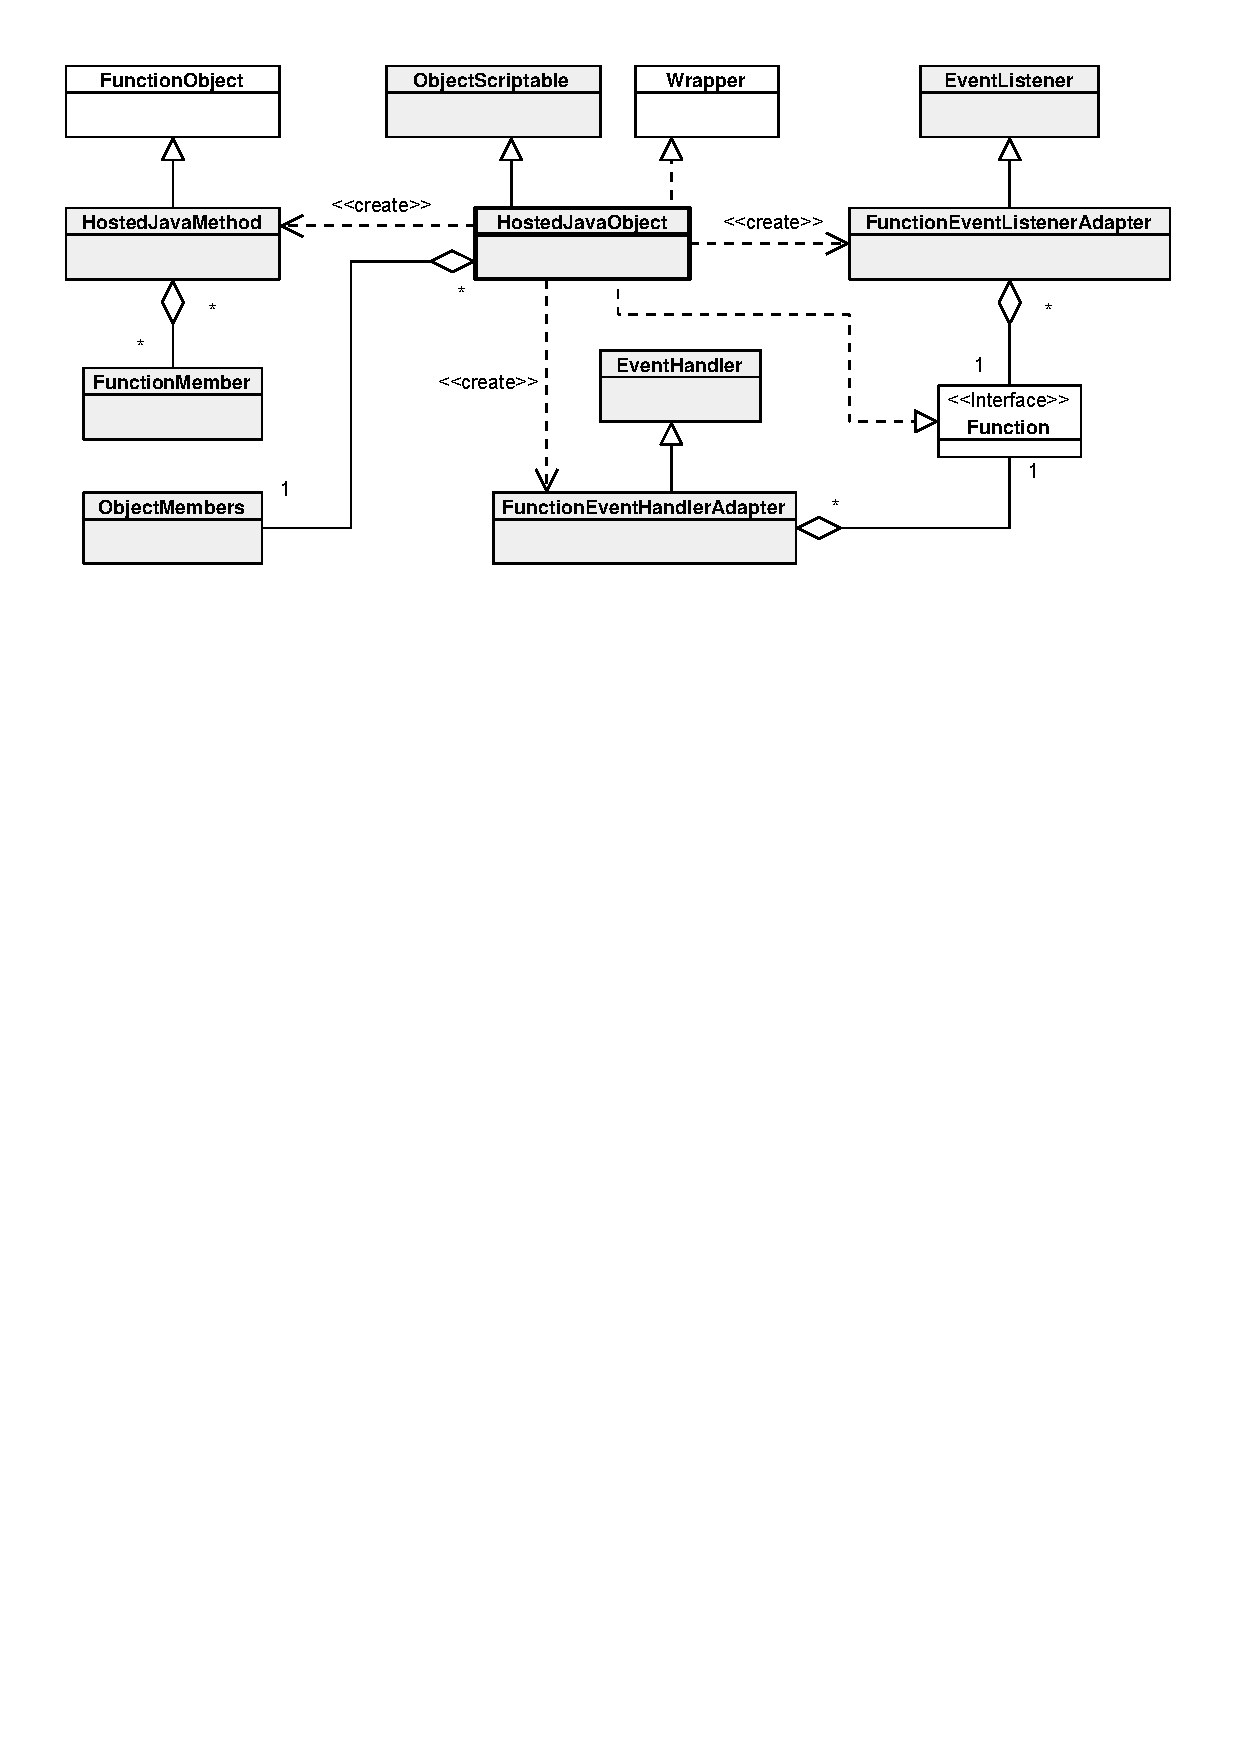
\includegraphics{fig/org-fit-cssbox-scriptbox-script-javascript-java-HostedJavaObject.pdf}
    }
    \caption{Diagram tříd znázorňující zapouzdřující objekt nativních objektů Javy}
    \label{Figure.HostedJavaObject}
  \end{center}
\end{figure}

\vspace{-1em}

Obalující objekt \texttt{HostedJavaMethod} rozšiřuje funkční objekt \texttt{FunctionObject} a~umožňuje uchovávat všechny přetížené metody, jež tento objekt představuje. Z důvodu volání přetížených metod, byla předefinována metoda \texttt{call()}, která se provádí při volání funkce. Při invokaci funkce dochází nejprve k vyhledání metody v~listu přetížených metod a~pak k zavolání vybrané metody. Bylo implementováno jednoduché vyhledávání metod metodou \texttt{getNearestObjectFunction()}, která vyhledává funkce na základě počtu argumentů a~jejich typů. Vyhledávání počítá i s možností volání metod s proměnnými argumenty.

Při nastavování nativních objektů JavaScriptu do některých rozhraní jádra uživatelského agenta, se naskytla potřeba některé tyto nativní objekty obalovat. V~diagramu na obrázku \ref{Figure.HostedJavaObject} vidíme, že např. obal \texttt{HostedJavaObject} může vytvářet adaptující objekty \texttt{FunctionEventHandlerAdapter} a~\texttt{FunctionEventListenerAdapter}. Tyto adaptéry jsou vytvářeny při požadavku na uložení nativní funkce JavaScriptu do některého z rozhraní \texttt{EventHandler} nebo \texttt{EventListener}. V~aktuální implementaci není momentálně jednotné místo, které by se staralo o správu těchto adaptérů.

Výše popsaný obal nativních objektů Javy \texttt{HostedJavaObject} je vytvářen v~rámci upravené obalující továrny \texttt{DafaultWrapFactoryDecorator} (obrázek \ref{Figure.WrapFactoryDecorator}). Vytvořená obalující továrna nově rozšiřuje třídu \texttt{WrapFactoryDecorator}, která umožňuje řetězení jednotlivých obalujících továren. 

\begin{figure}[H]
  \begin{center}
    \scalebox{0.75}{
      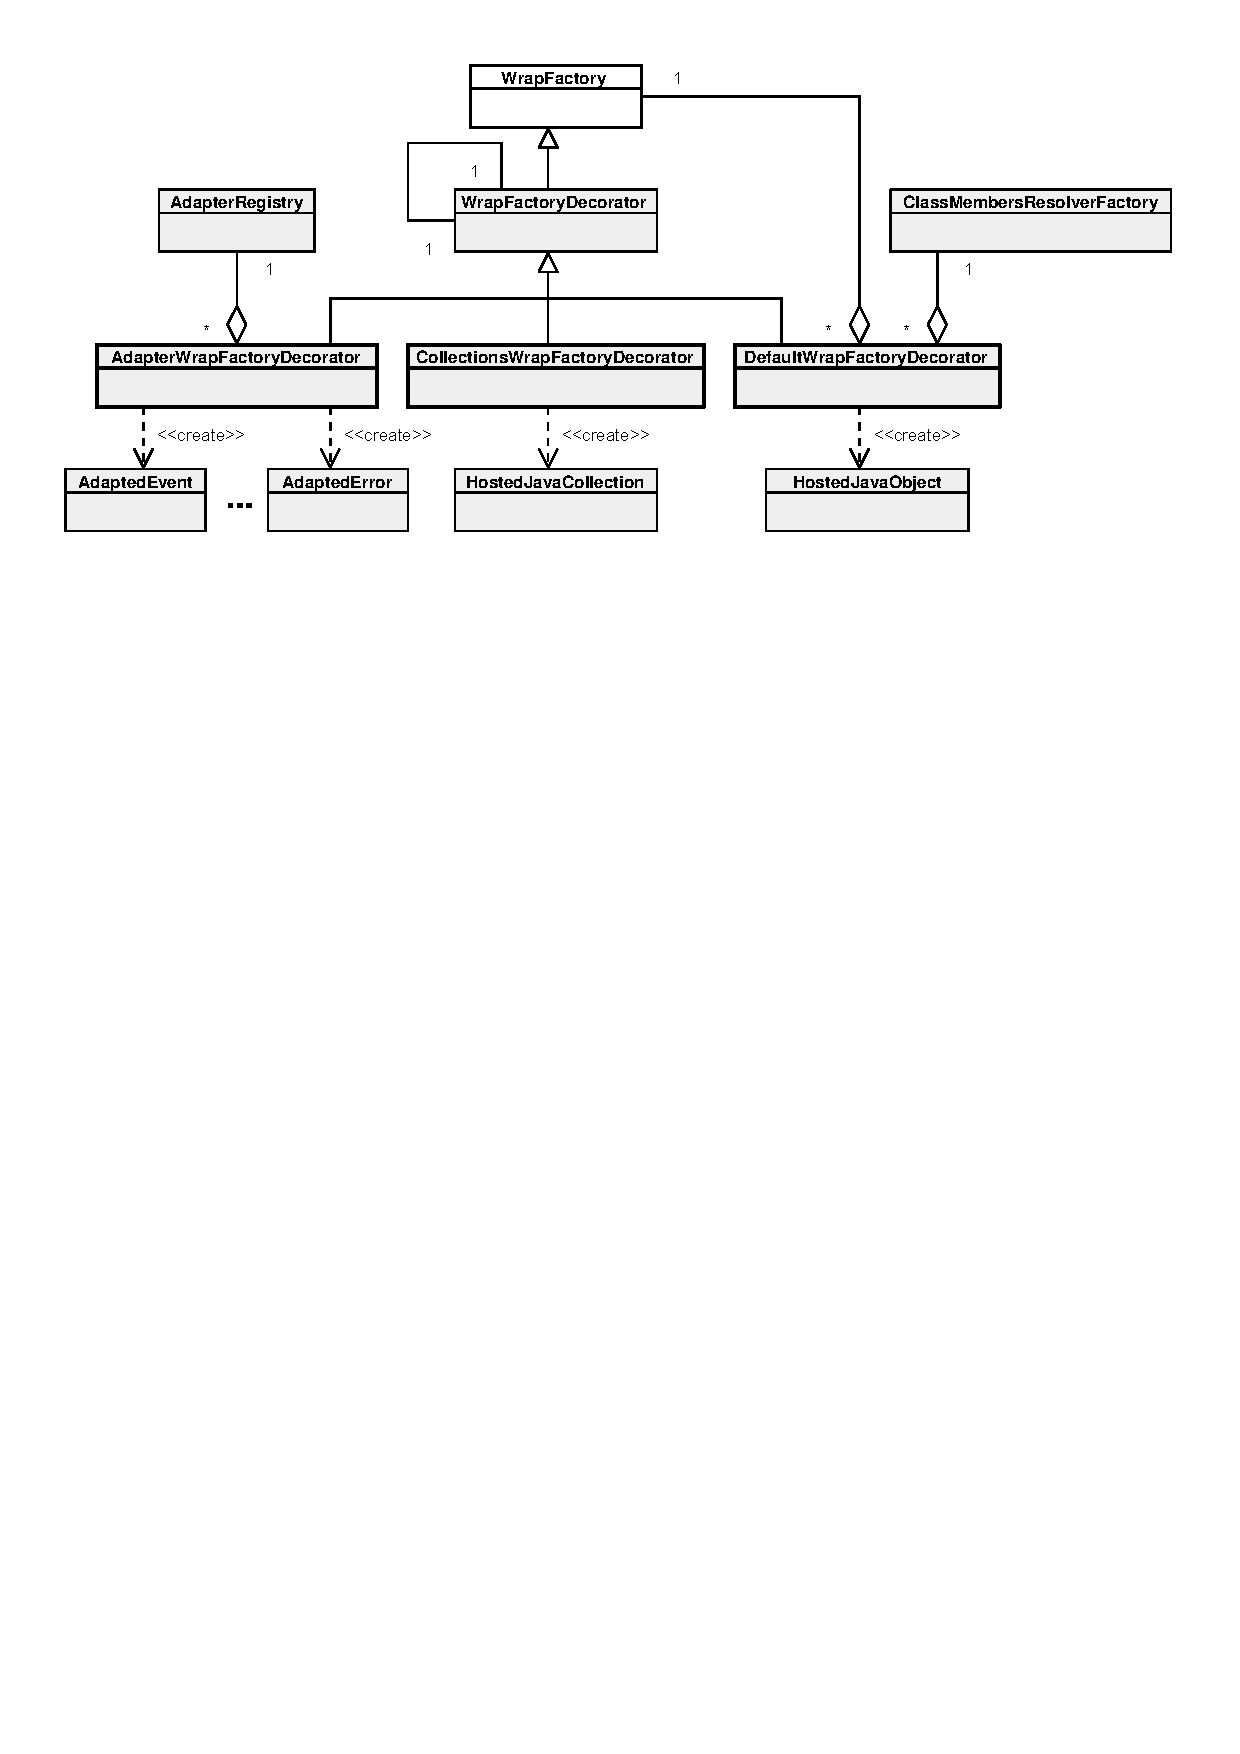
\includegraphics{fig/org-fit-cssbox-scriptbox-script-javascript-wrap-WrapFactoryDecorator.pdf}
    }
    \caption{Diagram tříd znázorňující obalující továrny}
    \label{Figure.WrapFactoryDecorator}
  \end{center}
\end{figure}

Pro JavaScriptový engine byly implementovány celkem tři obalující továrny, které se provádí v~následujícím pořadí:

\begin{enumerate}
  \item \textbf{\texttt{AdapterWrapFactoryDecorator}} -- obalující továrna převádějící nativní objekty, jež mají korespondující adaptér v~registru adaptéru, na adaptované objekty. Továrna vždy volá následující zřetězenou továrnu;
  \item \textbf{\texttt{CollectionsWrapFactoryDecorator}} -- obalující továrna převádějící nativní kolekce Javy na objekt HostedJavaCollection, čímž zpřístupňuje jejich prvky ve skriptech. Pokud není nativní objekt kolekcí, pak dochází k zavolání poslední zřetězené továrny;
  \item \textbf{\texttt{DafaultWrapFactoryDecorator}} -- obalující továrny provádějící převod všech nativních objektů na objekty \texttt{HostedJavaObject} tak, jak bylo popsáno výše.
\end{enumerate}

\section{Uživatelské rozhraní pro prohlížení stránek}
\label{Chapter.Implementation.UserInterface}

V~kapitole \ref{Chapter.Implementation.ContentHandling} jsme se zabývali zpracováním obsahu zdroje a~jeho převodem na dokument. Dalším krokem v~reálném prohlížeči by bylo zobrazení dokumentu uživateli a~to již během jeho parsování. Jelikož není hotova podpora pro inkrementální a~dynamické změny obsahu dokumentu, bylo implementováno zobrazování dokumentu až poté, co parser dokumentu dokončí svůj běh. Jednoduchou komponentu, která umožňuje prohlížení HTML dokumentů, implementuje třída \texttt{ScriptBrowser}. Komponenta vychází z komponenty \texttt{BrowserPane} implementované v~projektu SwingBox.

\begin{figure}[H]
  \begin{center}
    \scalebox{0.75}{
      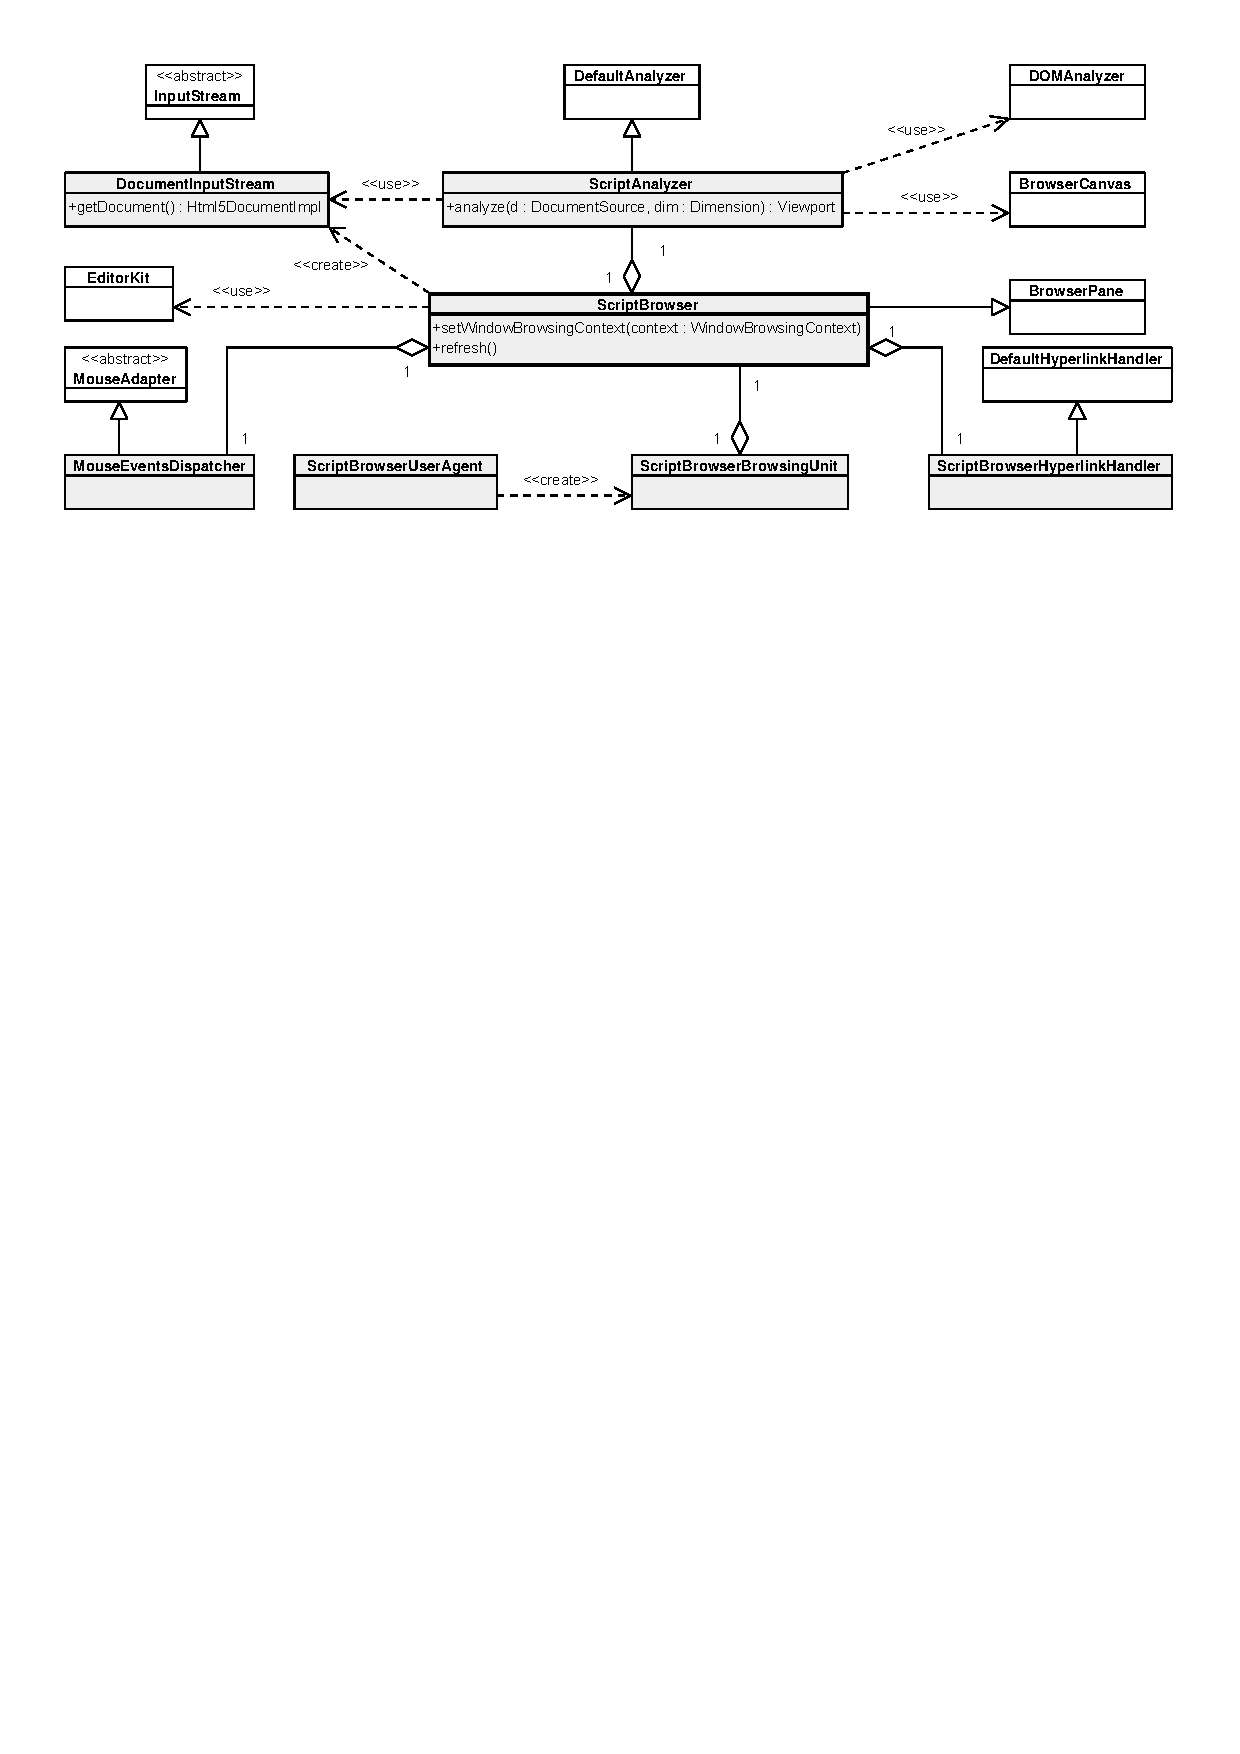
\includegraphics{fig/org-fit-cssbox-scriptbox-ui-ScriptBrowserUserAgent.pdf}
    }
    \caption{Diagram tříd znázorňující komponentu k vykreslování dokumentů}
    \label{Figure.ScriptBrowserUserAgent}
  \end{center}
\end{figure}

Třída \texttt{ScriptBrowser} zapouzdřuje procházecí kontext okna, nad kterým registruje odběratele pro události generované navigačním kontrolerem a~společnou historií sezení. Přijme-li odběratel událost, která znamená změnu dokumentu, pak tento odběratel volá metodu \texttt{refresh()}, jež způsobí vykreslení dokumentu. Během vykreslení dokumentu je získána reference na objekt \texttt{EditorKit}, nad nímž je zavoláno čtení dokumentu metodou \texttt{read()}. Jelikož dokument je již zpracován, tak metodě \texttt{read()} tento dokument předáme zapouzdřený do vstupního datového toku \texttt{DocumentInputStream}. Metoda \texttt{read()} vnitřně pro vykreslení dokumentu využívá instance \texttt{ScriptAnalyzer}, která byla s komponentou \texttt{ScriptBrowser} asociována během její konstrukce. V~rámci metody \texttt{analyze()} třídy ScriptAnalyzer dochází k  získání zapouzdřeného dokumentu ze vstupního datového toku, analyzování objektu DOM třídou \texttt{DOMAnalyzer} a~návrhu výsledného vzhledu dokumentu třídou \texttt{BrowserCanvas}.

Každá prohlížecí komponenta \texttt{ScriptBrowser} má asociovanou vlastní obslužnou rutinu pro to, co se má stát, když se klikne na URL odkaz. Obsluhu kliku na hyperlink implementuje třída \texttt{ScriptBrowserHyperlinkHandler}, která vnitřně volá navigační kontroler a~statickou metodu \texttt{followHyperlink()}. Kromě obsluhy URL odkazů, komponent implementuje generování událostí myši pro příslušné uzly dokumentu, nad kterými událost nastala. Jelikož komponenta může obsahovat posuvníky, informuje procházecí jednotka \texttt{ScriptBrowserBrowsingUnit} pomocí rozhraní \texttt{BarProp}, zda jsou posuvníky aktivni či nikoliv.

\section{Ukázkové aplikace}
\label{Chapter.Implementation.DemoApplications}

Pro znázornění funkčnosti uživatelského agenta byly implementovány dvě ukázkové spustitelné aplikace, které demonstrují jeho základní funkce. Obě aplikace sloužily k otestování možnosti prohlížet HTML dokumenty. Jejich implementace se nachází v~balíku projektu nazvaném \texttt{org.fit.cssbox.scriptbox.demo}.

Jednoduchá aplikace, která umožňuje pouze navigování stránek a~procházení společné historie sezení, je podrobněji popsána v~kapitole \ref{Chapter.Implementation.SimpleBrowser}. Další implementovanou aplikací, která přidává některé ladící komponenty klientského JavaScriptu, se zabývá kapitola \ref{Chapter.Implementation.JavaScriptTester}.  

\vspace{-0.5em}

\subsection{Jednoduchý prohlížeč}
\label{Chapter.Implementation.SimpleBrowser}

Pro vytvoření jednoduchého prohlížeče bylo zapotřebí definovat nového uživatelského agenta \texttt{SimpleBrowserUserAgent} (obrázek \ref{Figure.SimpleBrowserUiController}), který vytváří jednoduché procházecí jednotky \texttt{SimpleBrowserBrowsingUnit} obsahující uživatelské rozhraní. K implementaci jednoduchého uživatelského rozhraní bylo využito architektury MVP (model-view-presenter) s pasivním pohledem. Presenter v~implementaci představuje třída \texttt{SimpleBrowserUIPresenter}, pohled třída \texttt{SimpleBrowserUI} a~model uživatelský agent \texttt{SimpleBrowserUserAgent}.

\begin{figure}[H]
  \begin{center}
    \scalebox{0.75}{
      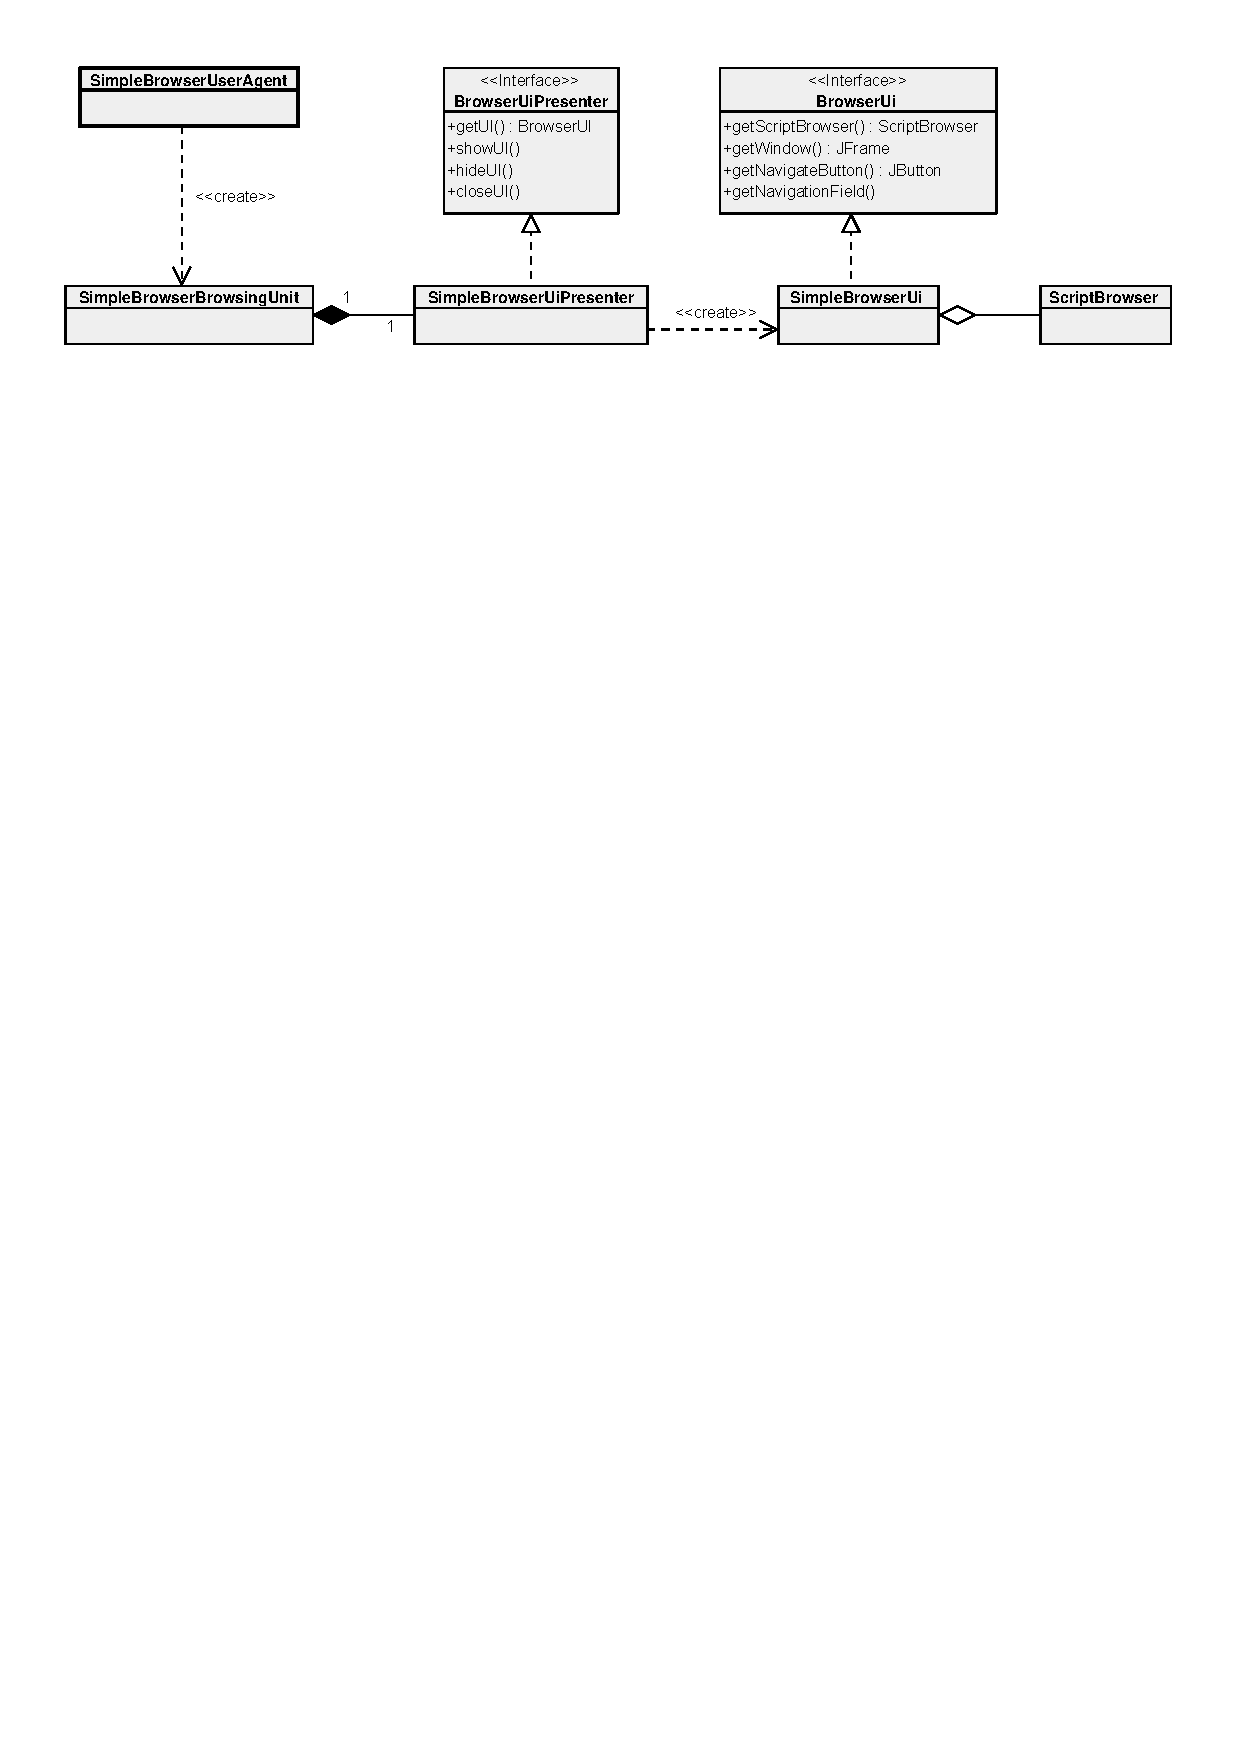
\includegraphics{fig/org-fit-cssbox-scriptbox-demo-browser-SimpleBrowserUiController.pdf}
    }
    \caption{Diagram tříd rozšíření uživatelského agenta o uživatelské rozhraní}
    \label{Figure.SimpleBrowserUiController}
  \end{center}
\end{figure}

\vspace{-1em}

Během konstrukce procházecí jednotky dochází nejprve k tvorbě presenteru, který v~rámci své tvorby vytváří pohled, se kterým je přímo spjat. Jakmile je pohled vytvořen, dochází presenterem k zaregistrování odběratelů událostí nad uživatelskými komponentami pohledu. Kromě odběratelů uživatelských komponent registruje presenter též odběratele u objektů uživatelského agenta, tzn. modelu. Konkrétně jsou zaregistrovány odběratelé nad navigačním kontrolerem hlavního procházecího kontextu a~nad společnou historií sezení procházecí jednotky. Po zachycení událostí z navigačního kontroleru nebo společné historie sezení dochází presenterem k pasivní úpravě pohledu. Při dokončení stažení dokumentu je např. aktualizován název~aplikace podle titulku stránky, po průchodu společnou historií sezení jsou aktualizovány tlačítka vpřed a~zpět.

Výsledný jednoduchý prohlížeč je zobrazen na obrázku v příloze \ref{Annex.SimpleBrowser}. Prohlížeč umožňuje navigovat nové stránky pomocí navigačního řádku a~procházet společnou historii sezení pomocí tlačítek vpřed a~zpět. 

\vspace{-0.3em}

\subsection{Tester JavaScriptu}
\label{Chapter.Implementation.JavaScriptTester}

Během testování funkčnosti uživatelského agenta se naskytla potřeba pro ladění klientských skriptů JavaScriptu -- vznik tzv. testeru. Z tohoto důvodu bylo implementováno rozšíření jednoduchého prohlížeče uvedeného v~předešlé kapitole \ref{Chapter.Implementation.SimpleBrowser}. Rozšíření přidalo ke komponentě pro prohlížení dokumentů další tři nové komponenty. Architektura pro tester byla zvolena také typu MVP. Presenter \texttt{JavaScriptTesterUIPresenter} využívá implementované funkčnosti v~presenteru \texttt{SimpleBrowserUIPresenter}. Vzhled testeru pohledu byl vytvořen zcela nový -- třída \texttt{JavaScriptTesterUI}. Vzhled implementuje rozhraní \texttt{BrowserUI} společné pro pohled jednoduchého prohlížeče.

První dvě komponenty, které byly navrženy a~zcela implementovány umožňují procházet objekty, které jsou definované ve skriptu. Na obrázku \ref{Figure.ScriptObjectViewerAndWatchList} můžeme vidět komponentu \texttt{ScriptObjectViewer} a~komponentu \texttt{ScriptObjectsWatchList}. 

\begin{figure}[H]
  \begin{center}
    \scalebox{0.75}{
      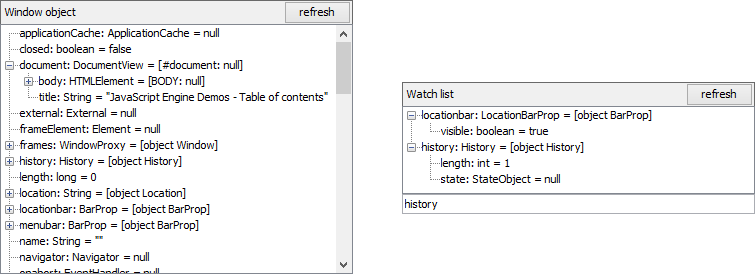
\includegraphics{fig/object-viewer-watch-list.png}
    }
    \caption{Komponenta \texttt{ScriptObjectViewer} (zleva) a~\texttt{ScriptObjectsWatchList}}
    \label{Figure.ScriptObjectViewerAndWatchList}
  \end{center}
\end{figure}

\vspace{-1em}

První komponenta \texttt{ScriptObjectViewer} umožňuje zobrazit všechny atributy objektu, který se jí předá. Společným objektem pro všechny klientské skripty je objekt \texttt{Window}, jehož bylo právě zvoleno pro výpis v~aplikaci testeru. Jednotlivé položky ve výpisu nelze ovlivnit a~jinak modifikovat. Komponenta je pouze informativní a~ukazuje aktuální stav~objektu \texttt{Window}.

Druhá komponenta \texttt{ScriptObjectsWatchList} přidává možnost volby objektů, které mají být ve výpisu objektů vypsány. Objekty lze kdykoliv~přidávat nebo je odebírat.  

Třetí komponenta (obrázek \ref{Figure.SourceCodeComponent}) slouží k procházení staženého zdrojového kódu dokumentu a~k jeho případné modifikaci. Pro zvýraznění syntaxe byla použita získaná knihovna jsyntaxpane. V~rámci komponenty lze dále vytvářet záložky, do kterých můžeme vkládat zdrojový kód, jenž je možno uložit nebo navigovat. Navigace vytvořeného zdrojového kódu probíhá tak, že se zdrojový kód uloží do složky dočasných souborů, ze které probíhá samotná navigace. 

\begin{figure}[H]
  \begin{center}
    \scalebox{0.50}{
      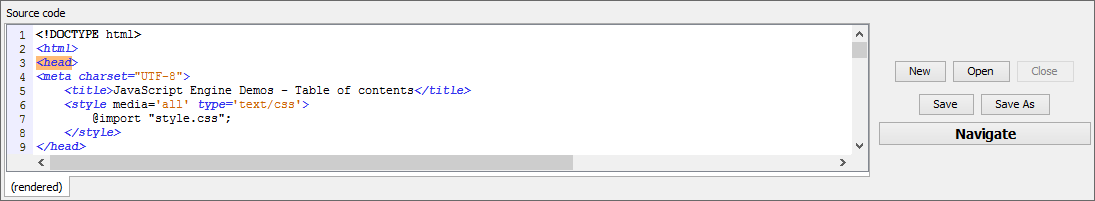
\includegraphics{fig/source-code.png}
    }
    \caption{Komponenta pro zobrazování zdrojového kódu dokumentu}
    \label{Figure.SourceCodeComponent}
  \end{center}
\end{figure}

\vspace{-1em}

\noindent Výsledná podoba aplikace je znázorněna na obrázku v~příloze \ref{Annex.JavaScriptTester}.

\chapter{Testování a dosažené výsledky}
\label{Chapter.TestingAndResults}

Následující kapitola se věnuje testování implementovaného řešení rozšíření projektu SwingBox a hodnotí jeho výkonost či kompatibilitu. První podkapitola \ref{Chapter.Testing} se zaměřuje na způsob,  jakým testování probíhalo, a uvádí testované aspekty řešení.  Další podkapitola \ref{Chapter.Performance} hodnotí výsledné řešení z hlediska výkonnosti. Míry ukazatele výkonnosti jsou porovnány s nejznámějšími prohlížeči. V závěru kapitoly jsou shrnuty dosažené výsledky, zhodnocena kompatibilita a uvedeny některé další možnosti, jakými by mohl v budoucnu pokračovat další vývoj celého projektu.

\section{Testování řešení}
\label{Chapter.Testing}

Testování implementovaného řešení probíhalo více způsoby. Funkčnost byla testována během celého vývoje rozšíření. Některé testy byly automatizovány a nyní se nachází v balíku tests. Automatizované testy byly vytvořeny pro otestování událostní smyčky, jednotlivých resolverů členů tříd a zapouzdřujících objektů nativních objektů Javy. Dodatečně byla funkčnost ověřena pomocí benchmarku SunSpider a ukázkovými HTML stránkami vytvořenými pro ukázkové aplikace zahrné v rozšíření.

V jednoduchých testech funkce událostní smyčky \texttt{EventLoopTests} byly vytvořeny tři testovací případy, které ověřují nejdůležitější funkčnost událostní smyčky. První případ \texttt{TestSpinEventLoopOrder} testuje, zda dochází ke správnému přerušení právě probíhající úlohy, předpokládané rotaci událostní smyčky a opětovnému vložení úlohy do fronty úloh. Druhý případ \texttt{TestSpinEventLoopAbort} testuje možnost ukončení událostní fronty metodou \texttt{abort()}, což hraje důležitou roli při rušení procházecí jednotky. Poslední případ \texttt{TestRoundRobinScheduler} ověřuje správnou funkci plánovače úloh s kruhovým výběrem a testuje, zda dochází opravdu ke kruhovému vybírání úloh.

Další implementované testy \texttt{HostedJavaObjectTest} a \texttt{JavaScriptAnnotationTests} sloužily k otestování funkce implementátoru globálního scopu a exportu nativních objektů Javy. Byl otestován výchozí resolver členů tříd a resolver založený na skriptovacích anotacích. Testy byly cíleny k ověření správného vyjmenování výčtových vlastností, tzn. členů, jež měly nastavenou možnost \texttt{ENUMERABLE}. Dále se testovaly možnosti \texttt{FIELD\_GET\_OVERRIDE}, \texttt{FIELD\_SET\_OVERRIDE}, \texttt{CALLABLE\_GETTER} a \texttt{CALLABLE\_SETTER}. Testy u všech členů tříd zkontrolovaly jejich návratové hodnoty s předpokládanými hodnotami a ověřily, zda byl exportován správný počet vlastností. Všechny vlastnosti, které by neměly být vidět ve skriptech, byly otestovány na nedefinovanou hodnotu \texttt{undefined}.

\newpage

Poslední implementované testy \texttt{CollectionsWrapFactoryTests} ověřily správnou funkci konverze nativních kolekcí Javy na objekty, které umožňují přístup k prvkům kolekci pomocí indexů. 

Jak již bylo zmíněno, k otestování správné funkčnosti sloužil i benchmark SunSpider\footnote{\url{https://www.webkit.org/perf/sunspider/sunspider.html}}, který ověřil správnou implementaci JavaScriptového enginu podle normy JSR 223. Benchmark obsahuje řadu testů k ověření základní JavaScriptové množiny a vyhodnocení výkonnosti skriptovacího enginu (kapitola \ref{Chapter.Performance}).

Důležitou roli během testování představovaly ukázkové HTML stránky, které slouží pro demonstraci funkčnosti implementovaného rozhraní klientského JavaScriptu. Během tvorby ukázkových stránek se otestovaly všechny rozhraní, které tyto stránky využívaly. 

\bigskip \noindent Bylo zhotoveno celkem 6 ukázek znázorňujících následující stěžejní implementace:

\begin{enumerate}
  \item \textbf{\texttt{dialogs.html}} -- představení základních uživatelských dialogů,
  \item \textbf{\texttt{events.html}} -- ukázka generování některých DOM událostí,
  \item \textbf{\texttt{scripts.html}} -- spouštění skriptů v rámci dokumentu,
  \item \textbf{\texttt{history.html}} -- procházení historií sezení,
  \item \textbf{\texttt{location.html}} -- navigovaní dokumentů,
  \item \textbf{\texttt{sunspider.html}} -- vnoření dokumentu pomocí značky \texttt{<iframe>}.
\end{enumerate}

\section{Vyhodnocení výkonnosti}
\label{Chapter.Performance}

Po dokončení implementace a jejím otestování byla vyhodnocena výkonnost implementovaného řešení. Pro všechny testy, které sloužily k vyhodnocení výkonnosti, bylo využito nezatíženého stroje, jehož výpočetní zdroje nebyly limitovány, např. nedostatkem operační paměti. Testovaná aplikace s implementovaných rozšíření byla přeložena překladačem EJC\footnote{\url{http://www.eclipse.org/jdt/core/}}. Pro testování sloužil stroj s operačním systémem Windows 8 a s následovnou základní konfigurací: Intel Core i5 2430M Sandy Bridge, RAM 4GB DDR3.

Pro vyhodnocení výkonnosti bylo využito benchmarku SunSpider, který obsahuje sadu základních výkonnostních testů. Jednotlivé testy jsou orientovány do řady vědních oborů a problémů reálného světa. Benchmark obsahuje například testy vykonávající kryptografické operace (SHA1, MD5, AES), sledování paprsku v prostoru (angl. 3D ray tracing), dekompresi spustitelného kódu aj.

Abychom mohli získané výsledky benchmarku porovnat s námi naměřenými hodnotami, bylo provedeno nejprve měření pro nejpoužívanější internetové prohlížeče. Vyhodnocenými prohlížeči jsou: Firefox, Chrome, Internet Explorer (dále IE) a Opera. Pro získání naměřených hodnot bylo využito veřejně přístupného API pro spuštění jednotlivých testů benchmarku. Každý test byl spuštěn celkem 5 krát. Získané časy trvání pro jednotlivé skupiny testů a pro všechny zmíněné prohlížeče lze vidět na obrázku \ref{Figure.BrowsersComparison}.

Z předešlého grafu bylo zjištěno, že výkonnosti jednotlivých skriptovacích enginů nejpoužívanějších internetových prohlížečů se výrazně neliší. Testy nejlépe dopadly pro prohlížeč FireFox, který všechny testy dokončil průměrně za 209 milisekund, a nejhůře pro prohlížeč IE, jehož testy trvaly průměrně $240$ milisekund.

\begin{figure}[H]
  \begin{center}
    \scalebox{0.60}{
      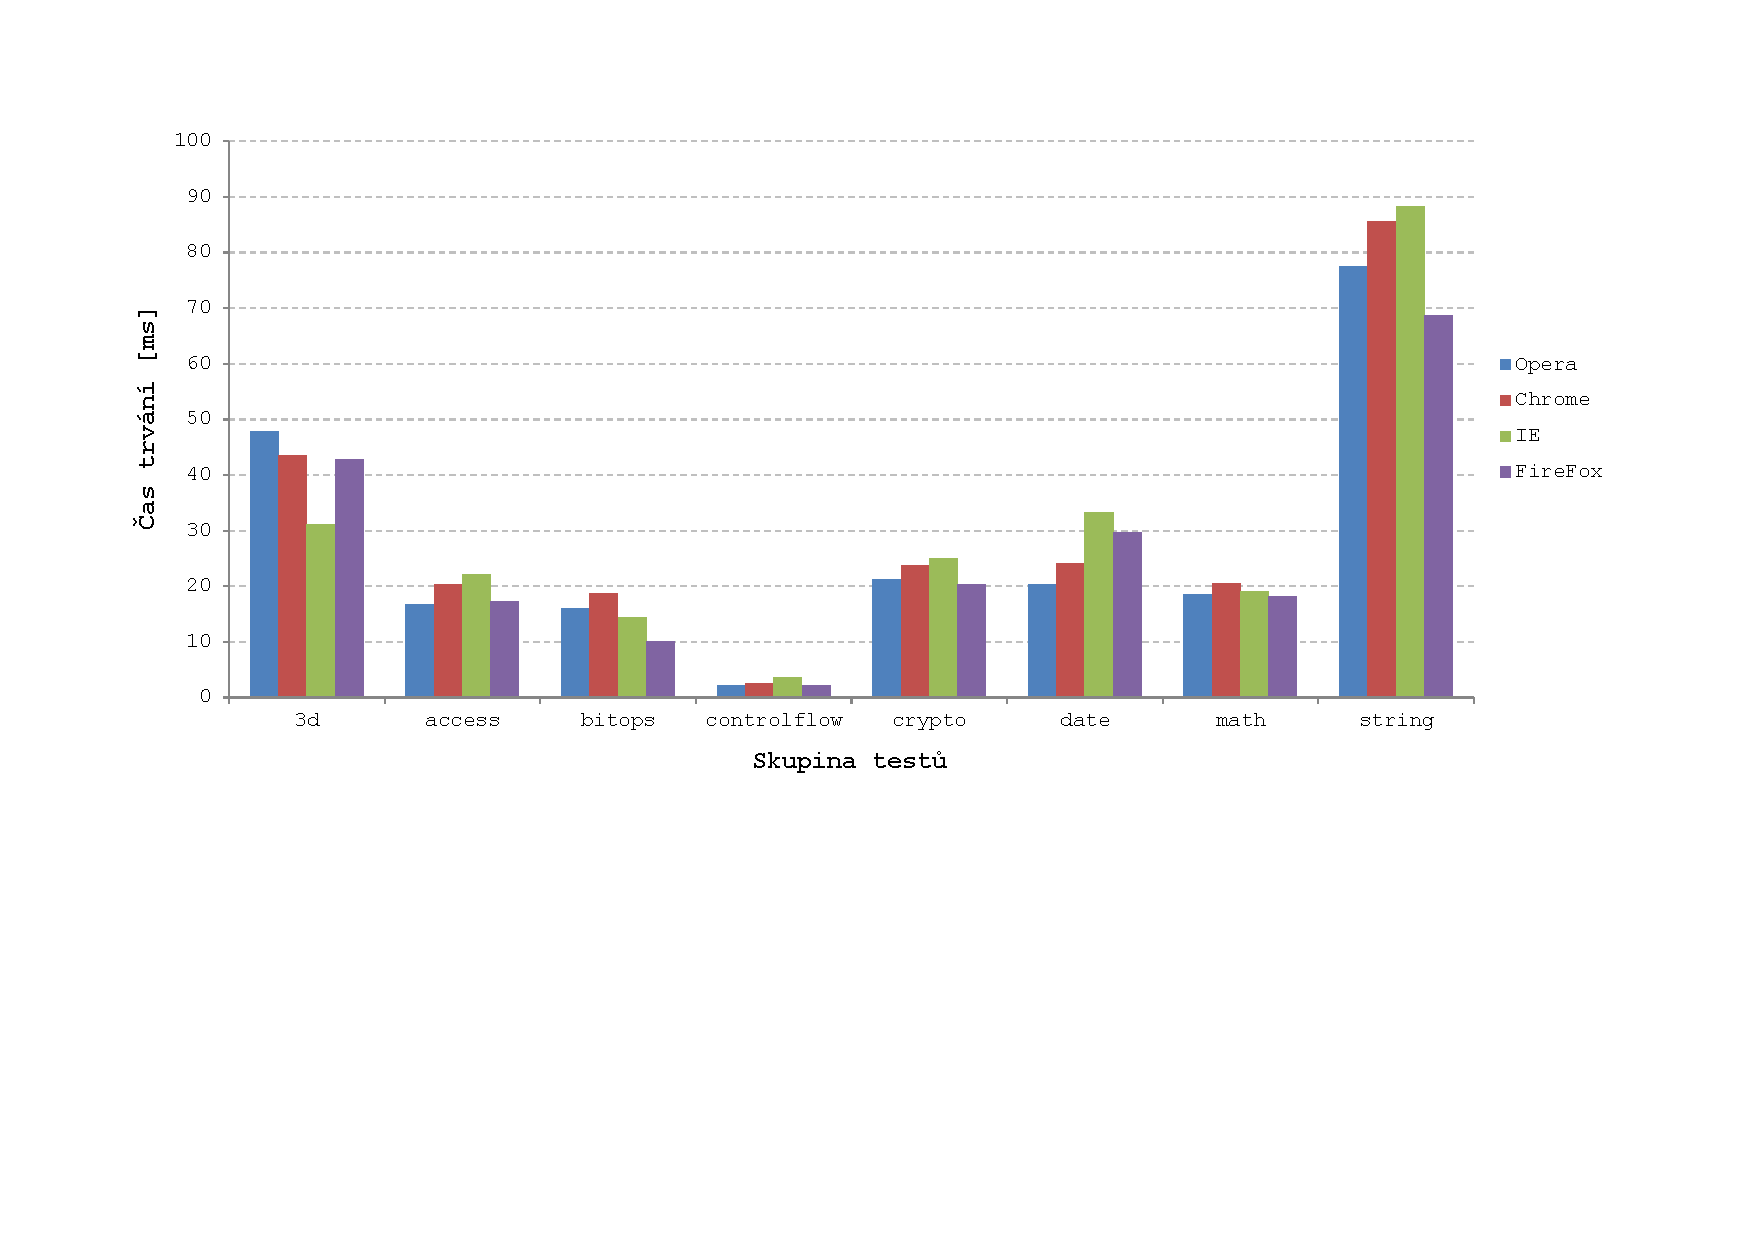
\includegraphics{fig/browsers-comparison.pdf}
    }
    \caption{Trvání jednotlivých skupin testů v prohlížečích}
    \label{Figure.BrowsersComparison}
  \end{center}
\end{figure}

\vspace{-1em}

Pro otestování námi implementovaného řešení bylo nutno vytvořit vlastní API benchmarku, které spouštělo jednotlivé výkonnostní testy. Veřejné API nebylo možné použít, jelikož pro svůj běh využívalo podmnožinu JavaScriptu, která nebyla doposud implementována. Vytvořené vykonávací API se nachází ve složce benchmark umístněné ve složce pro zdrojové kódy ukázkových HTML stránek (příloha \ref{Annex.dvdContent}). Implementované API získává ze zadané URL adresy dokument, který obsahuje seznam všech testů, jež by se měly vykonat. Skripty, jejichž cesty jsou uvedené v daném listu staženého dokumentu, se postupně jednotlivě vykonávají s předem známým počtem opakování.

\begin{figure}[H]
  \begin{center}
    \scalebox{0.60}{
      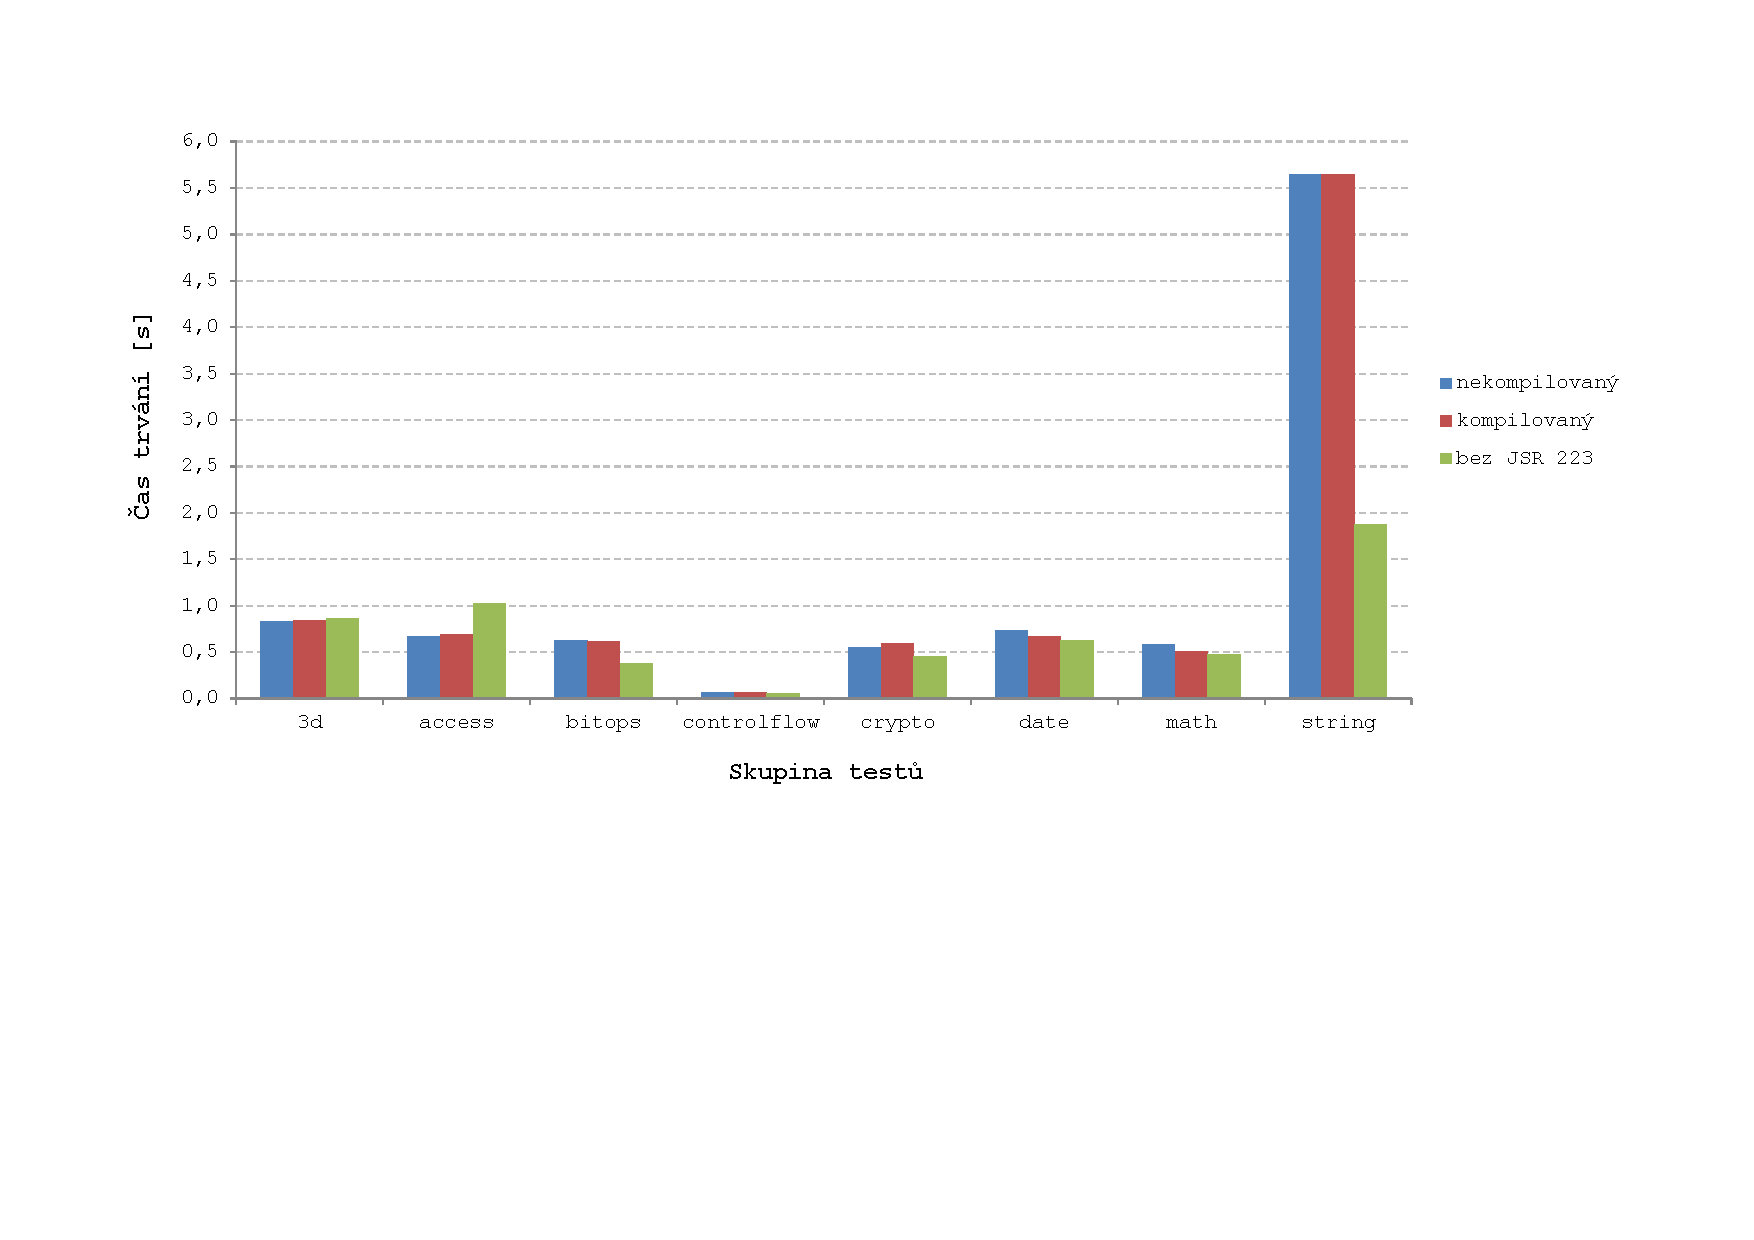
\includegraphics{fig/scriptbox-comparison.pdf}
    }
    \caption{Trvání jednotlivých skupin testů v implementovaném řešení}
    \label{Figure.ScriptBoxComparison}
  \end{center}
\end{figure}

\vspace{-1em}

Implementované řešení jsme nejprve sestavili tak, aby vykonávané skripty nebyly kompilovány před jejich spuštěním. Podruhé jsme řešení sestavili tak, že všechny skripty byly kompilovány. Nad oběma sestaveními jsme nechali běžet benchmark. Dále bylo provedeno několik experimentů, jelikož poslední skupina testů dopadla výrazně pod očekávání. Výsledkem experimentů bylo odstranění obalu ScriptContextScriptable, který zajišťoval data binding pro standardního skriptovacího API. Důsledkem odstranění obalu bylo např. znemožnění injekce skriptovacího kontextu. Tento zásah nepředstavoval žádný problém pro běh benchmarku. Nakonec jsme provedli i benchmark nad skriptovacím enginem, který neměl implementované rozhraní podle normy JSR 223. Výsledky všech tří běhů benchmarku jsou znázorněny na obrázku \ref{Figure.ScriptBoxComparison}. Každý test benchmarku byl spuštěn celkem $15$ krát a jeho doba trvání byla zprůměrována.

Získané časy trvání byly oproti ostatním internetovým prohlížečům výrazně delší. Kompilace skriptu neměla zásadní vliv na zrychlení běhu skriptu. Z důvodu „váznoucí“ poslední skupiny testů \texttt{string} byl celkový čas běhu jednoho benchmarku s kompilovaným nebo nekompilovaným kódem $9,6$ sekundy. Implementovaný skriptovací engine byl zhruba $42$ krát pomalejší než skriptovací enginy ostatních měřených internetových prohlížečů. Odstraněním standardního skriptovacího API došlo k výraznému zlepšení poslední skupiny testů \texttt{string}. V ostatních testovaných skupinách došlo taktéž k mírnému zlepšení. Celkový čas byl $5,7$ sekundy, což je $25$ krát pomalejší než průměrný celkový čas u dalších internetových prohlížečů. Problém vzniklý v poslední skupině \texttt{string} nebyl blíže trasován. Vysoká časová latence je s největší pravděpodobností způsobena převodem optimalizovaných textových řetězců JavaScriptu \texttt{ConsString} na nativní textové řetězece Javy \texttt{String}, který probíhá při každém uložení řetězce do globálního scopu.

\section{Zhodnocení řešení a jeho kompatibility}
\label{Chapter.RevaluationAndCompatibility}

Implementace navrženého řešení proběhla podle specifikace HTML 5.1, jež je stále ve fázi editorského návrhu. Stále rozšiřovaný a opravovaný dokument návrhu specifikace HTML 5.1 byl konfrontován se starší verzí specifikace HTML 5, která je již ve fázi doporučení. Až na některé výjimky lze říci, že dokončená množina podpory klientského JavaScriptu je kompatibilní se specifikací HTML 5.1. Všechny vzniklé nekompatibility byly vyznačeny v kódu odpovídajícím komentářem. Nekompatibility vznikly hlavně z důvodu nereentrantního parseru nebo jiné chybějící implementace. Mezi některé nejpodstatnější nekompatibility můžeme považovat např.:

\begin{enumerate}
  \item \textbf{neblokující spouštění skriptů} -- nebylo implementováno čekání na stažení kaskádových stylů dokumentu, které by mělo blokovat vykonávání skriptů. Stahování těchto zdrojů zajišťuje jiná třída v rámci projektu CSSBox. Abychom zabránili vícenásobnému stahování zdrojů, je nutné v budoucnu rozhraní projektů CSSBox a ScriptBox sjednotit. Zbylé požadavky na pořadí spouštění skriptů byly již implementovány přesně podle uvedené specifikace;
  \item \textbf{dialogs.html} -- aktuálně využívaný parser dokumentů NekoHTML není reentrantní. Chybějící funkčnost velice komplikuje případnou budoucí implementaci např. volání document.write(). Některé mechanismy, které ošetřovaly např. vnořené vložení \texttt{<script>} značky, nebyly kompletně implementovány, protože parser není reentrantní.
\end{enumerate}

V porovnání s předešlým projektem SwingBox, v němž chyběla implementace jádra uživatelského agenta, se snaží aktuální projekt věrně následovat specifikaci. Následně uvedeme některé případy, které vylepšují implementaci projektu SwingBox. 
 
V projektu SwingBox definovaná obslužná třída \texttt{DefaultHyperlinkHandler} pro klik na URL odkaz byla předefinována třídou \texttt{ScriptBrowserHyperlinkHandler}. Nová implementace obsluhy kliku na URL odkaz využívá jádra asociovaného uživatelského agenta, tzn. navigačního kontroleru pro navigování dokumentů. Díky změně implementace lze například odkazovat pomocné procházecí kontexty.

Projekt SwingBox implementoval stahování dokumentu v rámci událostní smyčky uživatelského rozhraní, což mělo za následek zablokování dané událostní smyčky a znemožnění práce s uživatelským rozhraním. Aktuální implementaci stahování dokumentu zajišťuje třída navigačního kontroleru, která naviguje dokument v asynchronním vlákně a pro jeho zpracování vkládá úlohu do událostní fronty aktuální procházecí jednotky. Celý proces stažení dokumentu a jeho zpracování probíhá v jiných vláknech než je vlákno uživatelského prostředí. Uživatelské rozhraní je nyní plně responsibilní.  

Implementace jádra uživatelského agenta probíhala podle jednotlivých podkapitol specifikace \cite{Bibliography.HTML5.TableOfContents}. Jmenovitě bylo čerpáno z následujících částí specifikace:

\begin{enumerate}
  \item \textbf{Webové aplikační API} \cite{Bibliography.HTML5.WebAPIs} -- využívané pro implementaci základních konceptů pro skripty \texttt{Script} a nastavení skriptů \texttt{ScriptSettings}. Část specifikace inspirovala také pro definici událostní smyčky \texttt{EventLoop}, událostí \texttt{Task} a jednoduchých uživatelských dialogů;
  \item \textbf{Načítání webových stránek} \cite{Bibliography.HTML5.Browsers} -- sloužilo pro implementaci procházecích jednotek, procházecích kontextů, navigování dokumentů a procházení historie sezení. Podkapitola specifikace též definovala rozhraní \texttt{Window}, \texttt{Location} a \texttt{History};
  \item \textbf{Skriptování} \cite{Bibliography.HTML5.Scripting} -- definovalo způsob zpracovávání elementů \texttt{<script>}, jejich převod na skripty \texttt{Script} a pořadí spouštění skriptů;
  \item \textbf{HTML syntaxe} \ref{Bibliography.HTML5.TheHtmlSyntax} -- sloužilo pro změnu NekoHTML parseru tak, aby správně zajišťoval spouštění parsovacích skriptů HTML dokumentu;
  \item \textbf{Společná infrastruktura} \cite{Bibliography.HTML5.Commoninfrastructure} -- inspirace pro způsob stahování zdrojů.
\end{enumerate}

Závěrem uvedeme kompletní implementovanou podmnožinu klientského JavaScriptu. Byla implementována následující podmnožina:

\begin{enumerate}
  \item \textbf{globální objekt} -- částečná implementace rozhraní \texttt{Window} (kapitola \ref{Chapter.Implementation.WindowInterface}),
  \item \textbf{navigování dokumentů} -- kompletní implementace rozhraní \texttt{Location} (kapitola \ref{Chapter.Implementation.DocumentNavigation}),
  \item \textbf{procházení historie} -- kompletní implementace rozhraní \texttt{History} (kapitola \ref{Chapter.Implementation.TraversingHistory}),
  \item \textbf{manipulace s URL} -- z větší části hotová implementace rozhraní \texttt{URLUtils} a \texttt{URL} (kapitola \ref{Chapter.Implementation.URLUtilsInterface}),
  \item \textbf{DOM události} -- jsou generovány některé události jádra uživatelského agenta, ale i události způsobené uživatelem, např. klikem na element dokumentu (kapitola \ref{Chapter.Implementation.DOMEvents}).
\end{enumerate}

\section{Možnosti budoucího vývoje}
\label{Chapter.PossibilitiesOfDevelopment}

Implementované řešení lze dále rozšiřovat. Možných cest dalšího vývoje vytvořeného rozšíření projektu SwingBox je celá řada. Následující vývoj by měl být cílen zejména na přidání další množiny funkčnosti klientského JavaScriptu. V některých částech již existující implementace je prostor pro různé optimalizace nebo pro dokončení a vylepšení funkčnosti. Malou část jednotlivé možností dalšího vývoje shrneme v následujícím seznamu. V některých případech naznačíme i možné řešení daného problému.

\bigskip \noindent Budoucí vývoj by se mohl zaměřit například na následující možnosti:

\begin{enumerate}
  \item \textbf{další podmnožina JavaScriptu} -- mělo by být implementováno např. rozhraní pro časovače, rozhraní \texttt{Navigator}, \texttt{ApplicationCache}, \texttt{External} aj.;
  \item \textbf{rozhraní objektu dokumentu} -- objekt \texttt{Window} v současné době obsahuje odkaz na dokument, který není zcela viditelný klientskému JavaScriptu. Rozhraní dokumentu implementuje pouze nejpodstatnější funkce, které bylo zapotřebí implementovat za účelem otestování některých částí uživatelského agenta. V budoucnu se předpokládá s odstraněním těchto metod z implementace dokumentu, kterou by mělo vidět pouze jádro uživatelského agenta, a vytvoření adaptéru nad tímto dokumentem. Adaptér by měl zpřístupnit viditelné rozhraní pro dokument v klientském kódu JavaScriptu. Vývojem viditelného rozhraní pro dokument se zabývala paralelně běžící diplomová práce Bc. Radima Kocmana. Pro propojení by stačilo vytvořit odpovídající adaptér a zaregistrovat ho do registru adaptérů \texttt{AdapterRegistry}. Do viditelného rozhraní by musely být přidány skriptovací anotace;
  \item \textbf{vylepšení WindowProxy} -- aktuální rozhraní \texttt{WindowProxy} slouží pro přístup ke globálnímu objektu \texttt{Window} aktivního dokumentu aktuálního procházecího kontextu. V implementaci rozhraní \texttt{WindowProxy} zpřístupňuje chování objektu \texttt{Window}. Podle specifikace by objekt \texttt{WindowProxy} měl mít chování zcela totožné jako objekt \texttt{Window}. V aktuální implementaci požadavku není zcela vyhověno, jelikož objekt \texttt{Window} a objekt \texttt{WindowProxy} jsou dvě odlišné instance. Implementačně proto selhává například operátor identity, neplatí \texttt{window === this}. Dalším problémem je, že definice nové proměnné uvnitř objektu \texttt{WindowProxy} se neprovádí v globálním scopu, ale ve scopu objektu \texttt{WindowProxy}. Problém by se dal vyřešit například předefinováním metody \texttt{shallowEq()} ve třídě \texttt{ScriptRuntime}. Tuto metodu vnitřně volá třída interpretu Rhina. Problémem je, že modifikace těchto tříd není veřejně přístupná. Přesměrování scopu objektu WindowProxy na globální scope aktivního objektu \texttt{Window} přepsáním metod \texttt{get()} a \texttt{set()} třídy \texttt{Scriptable};
  \item \textbf{mezipaměť pro členy tříd} -- při každém přístupu k nativnímu objektu Javy nyní dochází k vyhodnocování členů, jež by měly být exportovány do klientského JavaScriptu. Členy tříd pro již vyhodnocené třídy by bylo výhodné uchovávat v mezipaměti. Pro příští zapouzdření stejného nativního objektu Javy do objektu \texttt{HostedJavaObject} by se mělo využívat právě členů tříd uchovaných v této mezipaměti;
  \item \textbf{podpora \texttt{[Replaceable]}} -- k WebIDL atributu \texttt{[Replaceable]} v implementaci koresponduje zjednodušená možnost členů tříd \texttt{PERNAMENT}, kterou nyní resolver anotovaných členů tříd neumožňuje nastavovat a vynechávat. Možnost \texttt{PERNAMENT} je proto v aktuální implementaci vždy nastavena. S nenastavenou možností \texttt{PERNAMENT} nepředpokládá ani implementace pro obalování nativních objektu Javy do kódu JavaScriptu. Bylo by nutné udělat také podporu pro přepisování nativních členů tříd v expotovaných členů tříd nativních objektů Javy;
  \item \textbf{další události DOM} -- implementovat rozhraní pro nové DOM události, tak je definuje specifikace a ve správný okamžik je generovat. Chybí implementace například pro rozhraní \texttt{PageTransitionEvent} nebo \texttt{BeforeUnloadEvent};
  \item uvolňování dokumentu, ukončování právě spuštěných skriptů, podpora pro navigaci dalších URL schémat a jiných zdrojů než jsou HTML dokumenty.
\end{enumerate}

Před implementací některých z výše zmíněných rozšíření bude nutno nejprve zvážit a vyhodnotit, zda nebude výhodnější přejít na nový skriptovací engine Nashorn, který během vývoje této práce oficiálně vyšel společně s JDK 1.8. Přechod na nový skriptovací engine by obnášel novou implementaci podpory pro tento skriptovací engine. Muselo by se znovu řešit zapouzdřování nativních objektů Javy, implementace globálního scopu a jiná implementace nacházející se v balíku \texttt{org.fit.cssbox.scriptbox.script.javascript}.

Pokud by vývoj dále probíhal s enginem Nashorn, bylo by možné využít jeho podobného rozhraní pro všechny objekty JavaScriptu. Rhino pro všechny objekty JavaScriptu implementuje rozhraní \texttt{Scriptable}, Nashorn zavádí rozhraní \texttt{JSObject}. Jelikož jsou obě rozhraní sobě velmi podobná, lze tedy zvážit i vytvoření přemostění mezi knihovnou Rhino a Nashorn. Návrh přemostění je otázkou budoucího vývoje. Kompletní implementace nového podporovaného skriptovacího enginu by mohla probíhat obdobně tak jako skriptovacího engine Rhino.

\chapter{Závěr}
\label{Chapter.Final}

Cílem této diplomové práce bylo se seznámit s projektem CSSBox a~zanalyzovat problematiku skriptování v~jazyce JavaScript z jazyku Javy. Na základě získaných teoretických znalostí navrhnout architekturu a~způsob integrace skriptovacího stroje do projektu CSSBox. Dále tuto architekturu implementovat a zahrnout ji jako volitelné rozšiřitelní knihovny CSSBox. 

V~úvodní části textu bylo nejprve analyzováno skriptování v~HTML dokumentech a~referenční způsob pro přidání skriptovací podpory do dokumentu. Byl představen projekt CSSBox, do kterého proběhla integrace rozšíření, a~komponenta SwingBox pro zobrazování HTML dokumentu.

V~kapitole analýzy skriptovacích strojů byly demonstrovány existující řešení pro skriptování v~jazyce JavaScript v~Java aplikacích. Podrobně byla rozebrána technika tvorby skriptů s API knihovny Rhino. V~kontrastu na tvorbu skriptů s nestandardním API Rhina, byla ukázána i tvorba skriptu se standardním skriptovacím API Javy.

Návrh integrace rozšíření skriptování v~JavaScriptu přímo reflektoval teoretickou analýzu z předchozích kapitol. Z důvodu asynchronního spouštění skriptů jsme museli navrhnout inkrementální načítání dokumentu. Abychom odstranili potřebu měnit kód skriptovacího stroje při přidávání nového rozšíření hlavního scopu, jsme navrhli injektování do skriptovacího stroje s využitím injektáže závislostí. Jelikož knihovna Rhino obsahovala pouze základní kontrolu přístupu do Javy z JavaScriptu, navrhli jsme také třídy pro rozmělnění bezpečnosti a~lepší správu bezpečnostních politik. Závěrem návrhu jsme demonstrovali příklad „registrace“ samotného rozšíření do projektu SwingBox.

Po abstraktním návrhu je v práci popsáno konkrétní implementované řešení. Bylo implementováno jednoduché jádro uživatelského agenta. Jádro umožnuje stahovat předem neznámé typy zdrojů. V závislosti na typu komunikačního protokolu dochází k požadované obsluze zdroje. Stažené zdroje jsou jádrem dále zpracovávány a převáděny na objekty (X)HTML dokumentů. O převod se stará obecný mechanismus, který je adaptivní v závislosti na typu obsahu, jenž byl ze zdroje stažen. V jádře byl implementován proces navigace dokumentů, který využívá předešle zmíněnou funkčnost na stažení obsahu dokumentu a jeho zpracování. Dokumenty lze jádrem procházet díky zabudované historii sezení, která je unikátní pro každý procházecí kontext. V jádře byl implementován základní mechanismus pro generování DOM událostí, přičemž některé události jsou již nyní jádrem generovány. Jádro též zajišťuje spouštění skriptů. Byly implementovány všechny typy spouštění skriptů podle specifikace HTML 5. Skripty mohou být spuštěny v pořadí během parsování dokumentu, po dokončení parsování dokumentu nebo případně po načtení celého dokumentu. Implementována je podpora i pro asynchronní spouštění skriptů a dynamické vkládání skriptů do dokumentu.

Výše popsaná funkčnost jádra uživatelského agenta sloužila pro implementaci základních viditelných rozhraní JavaScriptu, jako jsou např.: \texttt{Location}, \texttt{History}, \texttt{Window}, \texttt{URL}, \texttt{URLUtils} aj. Rozhraní JavaScriptu jsou silně spjata s jádrem, zatímco jádro samotné s nimi minimálně. Rozhraní byla do klientského JavaScriptu exportována z nativních objektů Javy. Export nativních objektů zahrnoval prohledání tříd nativních objektů a rozhodnutí, zda má být člen tříd exportován či nikoliv. Prohledávání a vyhodnocení exportovatelných členů tříd bylo implementováno s využitím reflexe Javy a speciálních anotací, které značily exportovatelnost.

Implementovaný klientský JavaScriptový engine využívá navržené abstraktní architektury pro skriptovací enginy. Provádění skriptů zajišťuje knihovna Rhino, která byla rozšířena o standardní skriptovací API. Vytvořený klientský skriptovací engine umožňuje implementaci globálního objektu JavaScriptu do globálního scopu a export nativních objektů Javy. Během implementace enginu byl brán ohled na bezpečnost. Z tohoto důvodu byly některé funkce knihovny Rhino zcela vynechány nebo předefinovány.

Závěrem diplomové práce byly zhodnoceny dosažené výsledky a provedeno testování implementovaného rozšíření. V rámci výkonnostních testů bylo zjištěno, že interpret Rhino je značně pomalejší než interprety nejpoužívanějších internetových prohlížečů. Poslední kapitola práce se věnovala možným budoucím rozšíření této práce.
